%%%%%%%%%%%%%%%%%%%%%%%%%%%%%%%%%%%%%%%%%
% Arsclassica Article
% LaTeX Template
% Version 1.1 (1/8/17)
%
% This template has been downloaded from:
% http://www.LaTeXTemplates.com
%
% Original author:
% Lorenzo Pantieri (http://www.lorenzopantieri.net) with extensive modifications by:
% Vel (vel@latextemplates.com)
%
% License:
% CC BY-NC-SA 3.0 (http://creativecommons.org/licenses/by-nc-sa/3.0/)
%
%%%%%%%%%%%%%%%%%%%%%%%%%%%%%%%%%%%%%%%%%

%----------------------------------------------------------------------------------------
%	PACKAGES AND OTHER DOCUMENT CONFIGURATIONS
%----------------------------------------------------------------------------------------

\documentclass[
10pt, % Main document font size
a4paper, % Paper type, use 'letterpaper' for US Letter paper
oneside, % One page layout (no page indentation)
%twoside, % Two page layout (page indentation for binding and different headers)
headinclude,footinclude, % Extra spacing for the header and footer
BCOR5mm, % Binding correction
]{scrartcl}

\usepackage[
nochapters, % Turn off chapters since this is an article        
beramono, % Use the Bera Mono font for monospaced text (\texttt)
eulermath,% Use the Euler font for mathematics
pdfspacing, % Makes use of pdftex’ letter spacing capabilities via the microtype package
dottedtoc % Dotted lines leading to the page numbers in the table of contents
]{classicthesis} % The layout is based on the Classic Thesis style

\usepackage{arsclassica} % Modifies the Classic Thesis package

\usepackage[T1]{fontenc} % Use 8-bit encoding that has 256 glyphs

\usepackage[utf8]{inputenc} % Required for including letters with accents

\usepackage{graphicx} % Required for including images
\graphicspath{{Figures/}} % Set the default folder for images

\usepackage{enumitem} % Required for manipulating the whitespace between and within lists

\usepackage{lipsum} % Used for inserting dummy 'Lorem ipsum' text into the template

\usepackage{subfig} % Required for creating figures with multiple parts (subfigures)

\usepackage{amsmath,amssymb,amsthm} % For including math equations, theorems, symbols, etc
\usepackage{placeins}
\usepackage{graphicx}
\usepackage[italian]{babel}
\usepackage{varioref}

\theoremstyle{plain}
\newtheorem{teorema}{teorema}
\theoremstyle{plain}
\newtheorem{esercizio}{esercizio}
\theoremstyle{plain}
\newtheorem{applicazione}{applicazione}
\theoremstyle{plain}
\newtheorem{osservazione}{osservazione}
\theoremstyle{plain}
\newtheorem{assioma}{assioma}
\theoremstyle{plain}
\newtheorem{postulato}{postulato}
\theoremstyle{plain}
\newtheorem{corollario}{corollario}[teorema]
\theoremstyle{plain}
\newtheorem{lemma}[teorema]{lemma}
\theoremstyle{definition}
\newtheorem{definizione}{definizione}
\theoremstyle{definition}
\newtheorem{dimostrazione}{dimostrazione}
\theoremstyle{plain}
\newtheorem{esempio}{esempio}
\theoremstyle{plain}
\newtheorem{proposizione}{proposizione}
\makeatletter
\def\d{\ensuremath\partial}
\def\d{\ensuremath\partial\ }
\def\n{\ensuremath\nabla}
\def\n{\ensuremath\nabla\ }
\def\th@plain{%
	\thm@notefont{}% same as heading font
	\itshape % body font
}
\def\th@definizione{%
	\thm@notefont{}% same as heading font
	\normalfont % body font
}
\hypersetup{
colorlinks=true, breaklinks=true, bookmarks=true,bookmarksnumbered,
urlcolor=webbrown, linkcolor=RoyalBlue, citecolor=webgreen, % Link colors
pdftitle={}, % PDF title
pdfauthor={\textcopyright}, % PDF Author
pdfsubject={}, % PDF Subject
pdfkeywords={}, % PDF Keywords
pdfcreator={pdfLaTeX}, % PDF Creator
pdfproducer={LaTeX with hyperref and ClassicThesis} % PDF producer
} % Include the structure.tex file which specified the document structure and layout

\hyphenation{Fortran hy-phen-ation} % Specify custom hyphenation points in words with dashes where you would like hyphenation to occur, or alternatively, don't put any dashes in a word to stop hyphenation altogether

%----------------------------------------------------------------------------------------
%	TITLE AND AUTHOR(S)
%----------------------------------------------------------------------------------------

%\title{\normalfont\spacedallcaps{Fenomeni termici}} % The article title

%\subtitle{Subtitle} % Uncomment to display a subtitle

%\author{\spacedlowsmallcaps{Fabio Prestipino}} % The article author(s) - author affiliations need to be specified in the AUTHOR AFFILIATIONS block

%\date{Maggio 2022} % An optional date to appear under the author(s)

%----------------------------------------------------------------------------------------

\begin{document}
	\begin{titlepage}
		\begin{center}
			\vspace*{1cm}
			
			\Huge{\normalfont\spacedallcaps{Meccanica analitica classica}} % The article title
			
			\vspace{0.5cm}
			
			\vspace{1.5cm}
			
			\Large{\spacedlowsmallcaps{Fabio Prestipino}}
			
			\vspace{3.5cm}
			\LARGE{Un semplice riassunto per\\
				\textit{"sentire la musica"}}\\
			
			\vfill
			
			\vspace{2cm}
			\Large
			Fisica\\
			Università di Bologna\\
			Febbraio-Giugno 2023
			
		\end{center}
	\end{titlepage}
	
	%----------------------------------------------------------------------------------------
	%	HEADERS
	%----------------------------------------------------------------------------------------
	
	\renewcommand{\sectionmark}[1]{\markright{\spacedlowsmallcaps{#1}}} % The header for all pages (oneside) or for even pages (twoside)
	%\renewcommand{\subsectionmark}[1]{\markright{\thesubsection~#1}} % Uncomment when using the twoside option - this modifies the header on odd pages
	\lehead{\mbox{\llap{\small\thepage\kern1em\color{halfgray} \vline}\color{halfgray}\hspace{0.5em}\rightmark\hfil}} % The header style
	
	\pagestyle{scrheadings} % Enable the headers specified in this block
	
	%----------------------------------------------------------------------------------------
	%	TABLE OF CONTENTS & LISTS OF FIGURES AND TABLES
	%----------------------------------------------------------------------------------------
	
	%\maketitle % Print the title/author/date block
	
	\setcounter{tocdepth}{2} % Set the depth of the table of contents to show sections and subsections only
	
	
	
	%----------------------------------------------------------------------------------------
	%	AUTHOR AFFILIATIONS
	%----------------------------------------------------------------------------------------
	
	%\let\thefootnote\relax\footnotetext{* \textit{Dipartimento di Fisica, Università di Bologna}}
	
	%----------------------------------------------------------------------------------------
	
	\newpage % Start the article content on the second page, remove this if you have a longer abstract that goes onto the second page
	\tableofcontents % Print the table of contents
	\newpage
	%----------------------------------------------------------------------------------------
	%	INTRODUCTION
	%----------------------------------------------------------------------------------------
	
	
	
%\section{Introduzione concettuale: gli obiettivi e gli assiomi}
%Si immagini di essere un uomo primordiale, che non conosce nulla sulla realtà, sovrastato dalla complessità che lo circonda. Non è difficile immaginare necessità per quest'uomo di ridurre la realtà a sè stesso, di aggirare l'apparente casualità di ciò che lo circonda per uscire dall'iniziale stato di minorità in cui si versa. Ci si appella allora alla ragione, e si cerca di ricondurre il reale in termini razionali. Il fondamento della ragione è la logica, da essa discende la matematica che si fonda unicamente su postulati logici. La logica, mediata dalla matematica, è lo strumento con cui ridurre la realtà; la descrizione ottenuta in questo modo è inevitabilmente parziale perché è relativa a ciò che è quantificabile, cioè esprimibile in forma di numero. Inoltre, essendo l'uomo di dimensione trascurabile rispetto allo spazio in cui è contenuto, è necessaria l'ulteriore restrizione di considerare di volta in volta sistemi, cioè sottoinsiemi dell'inieme universo. Ciò che ci interessa è dunque trovare quantità che permettano di descrivere le caratteristiche quantificabili di un sistema. Quali caratteristiche quantificabili? Dipende da quale caratteristica quantificabile si vuole descrivere. Ad esempio, considerando un dado, se il nostro interesse è legato al numero che figura sulla faccia superiore, e nient'altro, allora lo stato del dado è descritto da un'unica variabile, esprimibile con un numero naturale, che può variare in un dominio che va da 1 a 6. Analogamente se di una moneta ci interessa quale delle due facce stia "all'in sù" possiamo descrivere lo stato del sistema con una variabile booleana che può assumere valori 0 o 1.
%\begin{definizione}[Stato di un sistema]
%	Lo stato di un sistema è un insieme di quantità che descrivono una o più delle sue caratteristiche quantificabili.
%\end{definizione}
%\begin{definizione}[Variabile di stato]
%	Le quantità necessarie alla descrizione dello stato di un sistema sono dette variabili di stato, esse hanno un dominio che può essere finito o infinito, sottoinsieme di un qualsiasi insieme nuemrico.
%\end{definizione}
%\begin{osservazione}
%	Il fatto di voler descrivere razionalmente la natura non implica che la natura sia razionale in sè, la ragione è una caratteristica non ben definita ma sicuramente propria dell'uomo, a priori. Altre ipotesi sulla razionalità intrinseca della realtà non sono escludibili ma senza ulteriori informazioni abbiamo solamente la certezza che la logica, fondamento della ragione, sia semplicemente la descrizione del funzionamento delle facoltà cognitive umane. Si parla spesso del fatto (a cui ci si appella per sostenere la razionalità intrinseca della natura) che la descrizione razionale della natura abbia portato a risultati tanto sorprendenti da suggerire che la natura effettivamente segua delle regole razionali a prescindere dall'uomo. Questo ragionamento per quanto non escludibile non offre alcun tipo di dimostrazione, sia perché il fatto che la ragione si adatti così bene alla descrizione della natura potrebbe essere giustificato con argomenti evoluzionistici, sia perché la descrizione della realtà a cui arriviamo è parziale, siamo stati noi a decidere cosa descrivere, sia perché ad oggi non è stata trovata una descrizione coerente neanche del pezzo di natura che ci siamo imposti di voler descrivere. Lo stupore riguardo i risultati della nostra descrizione della realtà fa spesso sovrastimare l'impresa stessa di questa descrizione, la fallacia fondamentale inquesto ragionamento è che l'apparente grandezza delle scienze naturali è tale in relazione alle capacità iniziali degli esseri umani, che partono da una condizione di totale ignoranza, ma non è grande in assoluto. Fino a prova contraria dunque lo scopo delle scienze naturali è quello di spiegare in termini razionali la natura; non è però detto che questa sia spiegabile in modo arbitrariamente preciso usando i mezzi della ragione, proprio perché fino a prova contraria non è intrinsecamente "costituita di ragione". Se la ragione non basta a descrivere la realtà allora cosa? Tutto ciò vorrebbe dire che la natura segue leggi che vanno oltre la ragione? Questo è un ragionamento fallace che presuppone che tutto ciò che è reale è razionale, e che anche se non fosse razionale rispetto all'uomo, lo è rispetto a qualche essere superiore. Si rifiuta in generale l'impossibilità di una descrizione razionale della realtà. Questa assunzione è ingiustificata ed è possibile che la ragione non sia semplicemente adatta a descrivere la natura superato un certo livello. Arrivati a questo punto non avrebbe senso chiedersi a quali regole, che esulano dalla ragione umana, la natura dovrebbe sottostare perché le regole presuppongono una ragione capace di comprenderle. A meno che non si accetti l'esistenza di un ente superiore rispetto al quale esistono delle legi di natura per esso ragionevoli ma per noi incomprensibili, assunzione molto forte ed in generale ingiustificata, allora bisogna accettare la possibilità, forse la probabilità, che la natura non sia riconducibile a principi razionali fino in fondo.\\
%	Una forte assunzione, spesso taciuta, che sta alla base della fede nella possibilità di descrivere razionalmente la realtà fino alla sua "radice" è quella che spesso viene chiamata "principio di ragion sufficiente"
%\begin{assioma}[Principio di ragion sufficiente]
%	La realtà è completamente descrivibile con i soli mezzi della ragione.
%\end{assioma}
%\end{osservazione}
%Tornando alla descrizione della realtà, risulta utile definire il sistema che ci interessa descrivere
%\begin{definizione}[Materia]
%	Definiamo materia tutto ciò che è percepibile dai sensi
%\end{definizione}
%\begin{definizione}[Sistema universo]
%	Il sistema universo è il sistema formato dalla totalità della materia esistente.
%\end{definizione}
%\begin{definizione}[Sistema fisico]
%	Un sottoinsieme della totalità della materia esistente è detto sistema fisico.
%\end{definizione}
%se vogliamo descrivere tutte le caratteristiche quantificabili dell'universo, o almeno di un suo sottoinsieme, cioè un sistema fisico, quali variabili di stato dobbiamo scegliere?\\
%Intuitivamente, se si vogliono descrivere tutte le caratteristiche di un sistema lo si dovrà decomporre nei suoi elementi fondamentali, che si ipotizza siano estremamente semplici, e che quindi è probabile possano essere descritti da un numero limitato di variabili, in questo modo se si riesce a definire in modo esaustivo lo stato di ogni singolo componente fondamentale della realtà si sarà ottenuta una descrizione completa di un sistema reale. Risulta chiaro che in questo ragionamento sono state fatte varie assunzioni che, si noti, erano centrali nei discorsi dei primi filosofi.
%\begin{assioma}[Esistenza dell'atomo]
%	La materia, e dunque l'universo, è formata da componenti di base non divisibili ulteriormente, detti atomi. 
%\end{assioma}
%Si osservi che in questo ambito l'atomo ha solo il significato di "costituente fondamentale della materia" e non quello usato nelle scienze, concernente protoni elettroni e neutroni. 
%\begin{assioma}[Semplicità della materia]
%	Lo stato del sistema composto da una singola particella è descrivibile da poche variabili di stato
%\end{assioma}
%Queste assunzioni sono forti ma non ci si ferma qui: osservando sperimentalmente che lo stato del sistema in cui viviamo muta, assumiamo l'esistenza del tempo. Il tempo è una quantità, condivisa da tutti i sistemi (a differenza di tutte le altre variabili di stato, che sono per definizione proprie del sistema) e dunque non definibile come variabile di stato, perché non propria del sistema, che parametrizza l'evoluzione di tutti i sistemi. In altre parole, il tempo è una variabile reale e ad ogni valore di questa variabile corrisponde uno stato del sistema universo, e dunque uno stato di ogni suo sottoinsieme.
%Ne segue che le variabili di stato di ogni sistema saranno funzioni del parametro tempo. Abbiamo dunque preso la seguente assunzione
%\begin{assioma}[Esistenza del tempo]
% Lo stato del sistema universo muta con continuità, dunque ad ogni stato è associabile un valore reale che chiameremo tempo. 
%\end{assioma}
%\begin{definizione}[Definizione operativa di tempo]
%	Il tempo è misurabile mediante un qualsiasi sistema che presenta una variabile di stato che varia in modo periodico, un periodo sarà un'unità di tempo.
%\end{definizione}
%Un requisito fondamentale delle nostre variabili di stato è che siano sufficienti a descrivere non solo una caratteristica quantificabile presente, come lo stato del dado o della moneta, ma che sia possibile, a partire dalla conoscenza di uno stato del sistema ad un dato tempo, di poter prevedere i suoi stati futuri e riscostruire i suoi stati passati; questo era lo scopo che l'uomo primordiale si era prefissato. La fede nel fatto che l'evoluzione del sistema sia totalmente descrivibile a partire dallo stato dato ad un istante di tempo, congiuntamente alla conoscenza delle leggi con cui evolve il sistema in funzione del tempo, è spesso individuata come l'assunzione fondamentale della posizione filosofica del determinismo
%\begin{assioma}[Determinismo]
%	A partire da una conoscenza infinitamente precisa delle variabili di stato di un sistema in un istante di tempo (condizioni iniziali) e delle leggi che regolano l'evoluzione del sistema nel tempo è possibile ricostruire tutti gli stati passati e prevedere tutti gli stati futuri.
%\end{assioma}
%\begin{osservazione}
%	\'E interessante il ruolo delle condizioni iniziali nella tesi meccanicista: costituiscono l'unico principio legato all'esperienza necessario per descrivere l'universo razionalmente. Per avere una descrizione completamente razionale bisognerebbe eliminare le condizioni iniziali, questa è stata la speranza (o almeno la fede che in un futuro sarebbe stato possibile farlo) di alcuni osi.
%\end{osservazione}
%\begin{osservazione}
%	Una posizione filosofica più forte del determinismo è il meccanicismo, per cui non solo la natura (e dunque tutto ciò che concerne la materia) è deterministica, ma ogni accadimento, anche "spirituale" (cade la distinzione fra materiale e spirituale in quest'ottica). In questa visione la conoscenza delle condizioni iniziali e delle leggi sarebbe sufficiente a descrivere l'evoluzione del sistema "essere umano" e dunque a prevederne i pensieri, i sentimenti, giudicati come riducibili di interazioni fra particelle. Risulta chiaro come questa posizione sia incompatibile con la concezione classica di libero arbitrio. Questa posizione è spesso accostata al materialismo, cioè la posizione filosofica secondo cui non esiste nient'altro di reale se non la materia, e dunque le particelle che compongono il sistema universo.
%\end{osservazione}
%Infine, perché l'impresa stessa della descrizione dell'evoluzione dello stato di un sistema fisico nel tempo abbia senso, è necessario che le leggi che descrivono l'evoluzione del sistema, in funzione del tempo siano in numero limitato, che non cambino nel tempo, e che siano le stesse per tutti i sistemi fisici. Se una di questi principi fosse violato, anche se esistessero, queste regole sarebbero inutili perché offrirebbero una descrizione tanto complessa della realtà da non adempiere allo scopo iniziale.
%\begin{assioma}[Semplicità delle leggi (principio di relatività)]
%	Le leggi che descrivono l'evoluzione nel tempo del sistema universo sono poche in numero, immutabili ed esprimibili con un numero esiguo di caratteri, le leggi infine hanno la stessa forma matematica in tutti i sistemi inerziali. Equivalentemente possiamo dire che tutti i S.R.I. sono fisicamente equivalenti.
%\end{assioma}
%Quanto detto fin ora è la base di tutta la fisica classica e relativistica, escludendo la fisica quantistica riguardo la quale il discorso è tutt'ora aperto e che va oltre lo scopo del presente testo. 
%Questi assiomi sono condivisi da tutte le formulazioni seguenti mentre gli assiomi che seguono cambiano a seconda della teoria adottata
%
%\section{Formulazione Newtoniana}
%\begin{assioma}[Tempo e spazio assoluti]
%	Il tempo e lo spazio non dipendono dal sistema fisico considerato.
%\end{assioma}
%\begin{definizione}[Spazio affine]
%	Intuitivamente lo spazio affine è uno spazio vettoriale in cui non vi è un punto centrale privilegiato e su cui è possibile definire l'operazione di "applicare un vettore a due punti". Il fatto che si usi uno spazio affine per costruire una teoria fisica è il fatto che non è importante quale sistema di riferimento si sceglie e quale sia la sua origine.
%\end{definizione}
%\begin{assioma}[Spazio]
%	Ogni particella occupa un punto di uno spazio affine reale tridimensionale. 
%\end{assioma}
%\begin{assioma}[Variabili di stato]
%	Per descrivere lo stato presente passato e futuro di un sistema è sufficiente la conoscenza di due variabili (sono rispettivamente vettori appartenenti a spazi vettoriali tridimensionali in generale diversi), di ogni particella costituente il sistema in un dato istante e delle leggi che governano la sua evoluzione nel tempo. Chiameremo queste variabili vettoriali posizione e quantità di moto. In generale queste sono funzioni del tempo.
%\end{assioma}
%\begin{definizione}[Coordinate]
%	Le coordinate sono un ennupla di numeri che individua un punto nello spazio.
%\end{definizione}
%\begin{definizione}[Sistema di coordinate]
%	Un sistema di coordinate è, fissato arbitrariamente un punto d'origine in cui le coordinate di questo punto saranno tutte nulle, l'insieme delle ennuple di numeri che individuano univocamente un punto nello spazio, rispetto al punto d'origine.
%\end{definizione}
%In meccanica newtoniana l'unico tipo di sistema di coordinate che si utilizza è quello cartesiano, cioè quello ottenuto dall'intersezione di tre rette ortogonali intersecantesi nell'origine. In particolare lo spazio che si considera è $\mathbb{R}^3$ con associata la metrica euclidea. La matrice metrica, che è la matrice associata al prodotto scalare di uno spazio, è la matrice identità 3x3.\\
%Un sistema rispetto a se stesso è chiaramente sempre in quiete ma un sistema osservato da un altro sistema di riferimento può essere in moto.
%\begin{definizione}[Posizione]
%	La posizione di un punto nello spazio è individuata dal vettore posizione dello spazio affine tridimensionale considerato, applicato all'origine. Le coordinate del punto saranno dunque i 3 valori assunti dalle componenti del vettore posizione. Si osservi come la posizione dipende inevitabilmente dal sistema di riferimento. In generale la posizione di un punto sarà funzione del tempo, cioè varierà al variare del parametro tempo.
%\end{definizione}
%\begin{definizione}[Velocità]
%	La velocità è il vettore ottenibile dalla derivazione nel tempo del vettore posizione.
%\end{definizione}
%\begin{definizione}[Accelerazione]
%	La'accelerazione è il vettore ottenibile dalla derivazione nel tempo del vettore velocità.
%\end{definizione}
%\begin{definizione}[Sistema di riferimento inerziale]
%	Un sistema di riferimento inerziale (S.R.I.) è un sistema di riferimento tale per cui una particella in moto rettilineo uniforme (con variabile di stato quantità di moto costante) non cambia la sua variabile di stato quantità di moto a meno che una causa indipendente dal S.R.I. non agisca su di essa. Chiameremo questa causa indipendente dal S.R.I. forza. Tutti i sistemi di riferimento che non rispettano questa caratteristica sono detti non inerziali. Tutte le variazioni si quantità di moto che non sono dovute ad una causa indipendente dal sistema di riferimento si dirà che sono dovute a forze non inerziali, dipendenti dalla variazione di momento nel tempo del sistema non inerziale rispetto ad un sistema di riferimento inerziale.\\
%	In altre parole, in un sistema inerziale lo spazio è omogeneo ed isotropo, ed il tempo è omogeneo, cioè per un punto materiale le leggi fisiche sono le stesse indipendentemente dalla posizione o dal verso in cui ci si sposta e dall'istante in cui si effettuano le misure. 
%\end{definizione}
%\begin{assioma}[Primo principio della dinamica]
%	Esiste un sistema di riferimento inerziale.
%\end{assioma}
%\begin{assioma}[Secondo principio della dinamica]
%	La variazione della quantità di moto di una particella nel tempo, in un S.R.I., è causata dalla forza mediante la seguente legge: sia F la forza e p la quantità di moto
%	\[\frac{dp(t)}{dt} = F\]
%	La forza è anch'essa una quantità vettoriale (tridimensionale). La forza è sempre esprimibile come variazione nello spazio (gradiente) di un campo scalare, detto potenziale, dipendente unicamente da posizione e tempo, che indichiamo come\( U(x, t)\) dunque possiamo scrivere
%	\[\frac{dp(t)}{dt} = \frac{\partial U(x, t)}{\partial x}\]
%	Inoltre il momento è legato alla posizione mediante la relazione
%	\[p = m \frac{dx}{dt}\]
%	oppure, ricordando la definizione di velocità
%	\[p = m v\]
%	La m che figura è una costante reale positiva detta massa, essendo tale possiamo riformulare il secondo principio della dinamica nella forma più nota
%	\[F = m a = m \frac{d^2x}{dt^2}\]
%	dove a è l'accelerazione. 
%\end{assioma}
%\begin{osservazione}
%	Cosa è la massa? Nell'ultima forma del secondo principio risulta più chiaro il ruolo della massa: nell'esperienza umana si osserva che una stessa causa (forza) riesce a far variare la velocità di un sistema (accelerazione) in quantità diversa a seconda di una caratteristica di cui abbiamo esperienza quotidiana e che chiamiamo massa. La massa è proprio la sensazione che proviamo quando sperimentiamo la difficoltà a far variare la velocità di un corpo quando noi siamo la fonte della causa (forza) che vuole farlo muovere. Si osservi che una stessa forza fa cambiare la quantità di moto di qualsiasi oggetto sempre della stessa quantità, indipendentemente dalla sua massa. 
%\end{osservazione}
%\begin{osservazione}
%	La forza è definita seguendo un principio di semplicità: non avendo informazioni su quale sia la causa della variazione del momento imponiamo che questa sia la forza e che sia proprio uguale alla variazione del momento nel tempo. Avremmo anche potuto definire la forza come la variazione del momento nel tempo al quadrato, avremmo potuto aggiungere costanti, ma sarebbe stata un'inutile complicazione. Inoltre bisogna notare la potenza di questo assioma: non è scontato che le due variabili di stato con cui descriviamo la realtà si trovino in relazione. Euristicamente, la posizione ci offre un'informazione sullo stato attuale del sistema, ma non tiene conto della variazione dello stato nel tempo; il momento è la variabile di stato che dentro di se contiene informazioni su come evolverà il sistema, infatti è definito mediante un rapporto incrementale in cui figura la variabile di stato posizione, calcolata in un istante di tempo infinitesimamente successivo a quello attuale. La struttura di questo principio rende essenzialmente qualunque problema fisico equivalente alla risoluzione di un'equazione differenziale in cui all'espressione \(\frac{\partial U(x, t)}{\partial x}\) del secondo principio, si sostituisce l'espressione del potenziale che agisce sul sistema. 
%\end{osservazione}
%\begin{osservazione}
%	Una volta appurata la relazione tra forza e variabili di stato, se riusciamo ad esprimere in formalismo matematico la forza, mediante il secondo principio della dinamica otteniamo una legge che descrive come le variabili di stato cambiano nel tempo, e dunque troviamo una legge che descrive l'evoluzione nel tempo del nostro sistema fisico. Per trovare la funzione con cui varia la posizione nel tempo otterremo così un'equazione differenziale del secondo ordine. In questo modo tutti i problemi fisici si riducono alla ricerca di forze e alla risoluzione delle equazioni differenziali.
%\end{osservazione}
%\begin{assioma}[Relatività galileiana]
%	Le leggi che descrivono l'interazione fra particelle hanno la stessa forma in tutti i sistemi di riferiemnto inerziali. Per passare da un sistema di riferimento inerziale ad un altro si usano le seguenti leggi di trasformazione (a meno di traslazioni): siano le quantità non accentate riferite ad una particella rispetto ad un S.R.I. K e quelle accentate rispetto ad un S.R.I. K', sia \(v_{K'}\) la velocità dell'origine di K' rispetto al S.R.I. K
%	\[x = x' + v_{K'} t\]
%	\[p = mv = mv' + mv_{K'} = p' + m v_{K'}\]
%	Essendo K' un S.R.I. la sua velocità è costante dunque derivando la quantità di moto rispetto ai due sistemi si ottiene lo stesso risultato
%	\[F = \frac{dp}{dt} = \frac{dp'}{dt} = F'\]
%\end{assioma}
%Il fatto di aver postulato l'esistenza di un sistema di riferimento inerziale, insieme al fatto che è possibile passare da un S.R.I. all'altro mediante le trasformazioni di galileo, implica l'esistenza di un'intera classe infinita di sistemi di riferimento inerziali, in moto rettilineo uniforme rispetto a quello esistente per ipotesi.\\
%Si noti che dal fatto che le accelerazioni sono uguali discende che, essendo la massa costante, anche le forze sono uguali, dunque le leggi con cui si evolve il sistema restano le stesse nel passare da un sistema di riferimento ad un altro, in accordo con il principio di relatività. La validità delle trasformazioni di galileo è legata alle assunzioni fatte in precedenza secondo cui spazio e tempo sono assoluti.
\section{Evoluzione del sistema e flusso di fase}
Il secondo principio della dinamica offre la possibilità di costruire equazioni differenziali, note le forze, la cui soluzione porta alla conoscenza delle equazioni del moto, ovvero alle funzioni che descrivono l'evoluzione nel tempo dello stato di un sistema fisico. Vogliamo formalizzare in modo il problema della risoluzione delle equazioni differenziali scaturenti dal secondo principio della dinamica (equazioni differenziali sono di tipo vettoriale). In questa sezione introdurremo la struttura matematica necessaria a formalizzare questi concetti.\\
Innanzitutto si vuole rappresentare l'insieme degli stati possibili di un sistema
\begin{definizione}[Varietà]
Spazio topologico di Hausdorff (cioè tale che per ogni coppia di punti esistono due aperti disgiunti che li contengono, separabile), su cui è definito un ricoprimento \[W = \{W_i\}\] di aperti tale che ogni aperto può essere posto in relazione con un aperto dello spazio euclideo mediante l'omeomorfismo (deformazione senza strappi, funzione continua, invertibile con inversa continua, per la definizione topologica di continuità porta aperti in aperti sia all'andata che a ritorno) \[\phi_i:W_i\rightarrow \mathbb{R}^n\] Intuitivamente, considerando varietà bidimensionali immerse nello spazio \(\mathbb{R}^3\), una varietà è una superficie liscia che localmente è approssimabile ad un piano.\\
\end{definizione}
\begin{definizione}[Spazio di stato]
	Uno spazio in cui sono rappresentate le possibili configurazioni dello stato di un sistema. 
\end{definizione}
\begin{definizione}[Spazio delle fasi]
	Lo spazio di stato in cui sono rappresentate quantità di moto e posizioni di un sistema è detto spazio delle fasi. Dato un sistema di n particelle, lo spazio delle fasi ha 6n dimensioni. Solitamente si rappresenta lo spazio delle fasi per sistemi formati da una sola particella vincolata a muoversi in uno spazio unidimensionale, in questo caso lo spazio delle fasi ha due dimensioni; in questo caso si rappresenta la quantità di moto sulle y e la posizione sulle x. Ad ogni punto dello spazio delle fasi corrisponde uno stato del sistema. L'insieme di tutti i possibili stati che un sistema può assumere sono rappresentati nello spazio delle fasi da una varietà, l'evoluzione nel tempo dello stato di un sistema sarà dunque una curva su questa varietà.
\end{definizione}
\begin{definizione}[Spazio delle configurazioni]
	Lo spazio di stato in cui figurano le posizioni è detto spazio delle configurazioni, questo ha 3n dimensioni, si rappresenta solitamente lo spazio delle configurazioni di una particella ponendo le 3 coordinate di posizione sui tre assi.  Ad ogni punto dello spazio delle configurazione corrisponde una posizione del sistema. L'insieme di tutte le possibili posizioni che un sistema può assumere sono rappresentati nello spazio delle configurazioni da una varietà, l'evoluzione nel tempo della posizione di un sistema sarà dunque una curva su questa varietà. Questa potrà essere parametrizzata dal tempo, che è un parametro speciale, perché ha anche un significato fisico, o da un generico parametro. Il primo approccio è detto dinamico, il secondo è detto geometrico. 
\end{definizione}
\begin{esempio}[Spazio delle configurazioni di un pendolo]
	Un pendolo è vincolato a muoversi su una sfera dunque il suo spazio delle configurazioni è una sfera, la sfera è una varietà differenziabile che localmente è approssimabile con un piano (la terra sembra piatta rispetto ad un essere umano di dimensioni trascurabili rispetto al raggio di curvatura).
\end{esempio}

\begin{definizione}[Flusso di fase]
	Il flusso di fase è una trasformazione dello spazio delle fasi (funzione) dipendente dal parametro reale $\alpha$ e dalle condizioni iniziali del sistema (sarebbero le condizioni per un qualsiasi valore di $\alpha$, che noi scegliamo come \(\alpha_0 = 0\). Inoltre il flusso di fase per definizione è tale che per $\alpha$ = 0 diventa la trasformazione identità, per ogni condizione iniziale, e che la composizione di due flussi di fase che evolvono un sistema di $\alpha_1$ e $\alpha_2$ equivale ad un flusso di fase che evolve il sistema di \(alpha_3 = \alpha_2 + \alpha_1\) \\
	Sia X lo spazio delle fasi:
	\[\Phi^{(\alpha)}(\mathbf{x}): \mathbb{R}\times X\rightarrow X\]
	\[\Phi^{(0)}(\mathbf{x}) = \mathbf{x}\]
	\[\Phi^{(\alpha_1)}(\mathbf{x})\circ \Phi^{(\alpha_2)}(\mathbf{x}) = \Phi^{(\alpha_1+\alpha_2)}(\mathbf{x})\]
\end{definizione}
	Considerando per chiarire le idee il caso di una singola particella: fissata una condizione iniziale il flusso di fase restituisce l'evoluzione dello stato sistema al variare del parametro $\alpha$, cioè restituisce \(\mathbf{x}(\alpha) = (x(\alpha), p(\alpha))\). Visto il significato fisico del flusso di fase risulta ovvio il motivo per cui per $\alpha = 0$ imponiamo che il flusso di fase sia l'identità: a partire dalle condizioni iniziali \((x_0, p_0)\), dopo una variazione nulla del parametro $\alpha$, il sistema non si è evoluto dunque il suo stato resta immutato.\\
	Possiamo vedere il flusso di fase come un propagatore delle condizioni iniziali. Si noti che il flusso di fase ha la forma di una matrice di trasformazione dipendente da $\alpha$ applicata al vettore delle condizioni iniziali; nel caso dello studio di una singola particella la matrice ed il vettore in questione sono in generale rispettivamente una matrice 6x6 ed un vettore appartenente ad uno spazio a sei dimensioni. (Tuttavia vedremo principalmente sistemi 1-D in cui la matrice è 2x2)
	Fissate le condizioni iniziali, il flusso di fase di una particella costituisce una curva sullo spazio delle fasi. Si faccia attenzione al fatto che in questo contesto $\mathbf{x}$ (in grassetto) rappresentazione la posizione della particella nello spazio delle fasi.
\begin{definizione}[Flusso]\label{def:flusso}
	Un caso particolare di flusso di fase è il flusso, cioè un flusso di fase che non dipende dai momenti. Differisce dal flusso di fase solo nel fatto di essere definito sullo spazio delle configurazioni e non sullo spazio delle fasi.
\end{definizione}
\begin{osservazione}[Cosa è \(\alpha\)?]
Se $\alpha$ è interpretato come il tempo, allora il flusso di fase definisce la dinamica del sistema, cioè l'evoluzione nel tempo dello stato del sistema. $\alpha$ però può essere più in generale un qualsiasi parametro, in questo caso si perde l'informazione sulla dinamica, cioè la successione temporale degli eventi, e si ottiene una visione geometrica. Ad esempio, se $\alpha$ è interpretato come l'angolo e il flusso di fase come una rotazione, allora fissata la condizione iniziale la funzione \(\Phi^{(\alpha)}(x_0)\) ci dice come evolve lo stato del sistema in funzione dell'angolo. Se poi parametrizziamo l'angolo con il tempo torniamo ad avere la dinamica.
\end{osservazione}
Si noti che il flusso di fase è la soluzione del problema di trovare le espressioni che descrivono l'evoluzione del nostro sistema. Lo scopo che ci poniamo è quello di impostare una equazione differenziale la cui soluzione sia il flusso di fase, sfruttando il secondo principio della dinamica.\\
Possiamo considerare la variazione nel tempo dello stato del sistema nello spazio delle fasi come conseguenza dell'esistenza di un campo vettoriale che associa ad ogni stato (cioè ad ogni punto dello spazio delle fasi), un vettore tangente allo spazio delle fasi. Per introdurre formalmente il campo vettoriale associato al flusso di fase bisogna innanzitutto definire la struttura matematica su cui vive
\begin{definizione}[Fibrato tangente]
	Data una varietà differenziabile $\Phi$, il fibrato tangente di questa, \(T_{\Phi}\), è l'unione disgiunta di tutti gli spazi tangenti ai punti di $\Phi$. Essendo lo spazio tangente individuabile da un punto sulla varietà e dall'insieme dei vettori tangenti alla varietà in quel punto, possiamo vedere un punto del fibrato tangente come (x, v, u, w, ...) dove x è un punto di $\Phi$ e gli altri vettori fanno parte dello spazio tangente alla varietà in x. 
\end{definizione}
\begin{osservazione}[Il fibrato tangente e lo spazio delle configurazioni]
	I vettori posizione fanno chiaramente parte dello spazio delle configurazioni, poiché questo è definito a partire dalle posizioni. Le velocità invece fanno parte del fibrato tangente alla varietà differenziabile definita dallo spazio delle configurazioni. La velocità è la derivata della posizione, la derivata di un vettore x su una varietà lo porta nello spazio tangente alla varietà nel punto x dunque la velocità sta nello spazio tangente ad un punto x, in generale lo spazio in cui stanno le velocità è l'unione degli spazi tangenti ai punti x della varietà, che è proprio la definizione del fibrato tangente.\\
	Indichiamo il fibrato tangente allo spazio X con \(T_X\)
\end{osservazione}
\begin{osservazione}[I momenti e il fibrato cotangente]
	In generale i momenti, come sarà chiaro in seguito, stanno nello fibrato cotangente allo spazio delle configurazioni, ovvero nel duale del fibrato tangente di questo spazio. Solo in formulazione cartesiana tuttavia lo spazio delle configurazioni, e il suo spazio tangente e cotangente coincidono (Lo spazio tangente o cotangente ad \(\mathbb{R}^3\) è \(\mathbb{R}^3\) stesso, cosa falsa per un generico spazio). In particolare, per il secondo principio della dinamica il momento associato alla posizione è il momento della quantità di moto, che è proporzionale alla velocità mediante la massa m, una costante. Bisogna far attenzione al fatto che questa relazione è valida solo in formulazione cartesiana.\\
	Indichiamo il fibrato cotangente allo spazio X con \(T^*_X\)
\end{osservazione}
\begin{definizione}[Campo vettoriale associato al flusso di fase]
	Il campo vettoriale
	\[a: X\rightarrow T_{X}\]
	che va dallo spazio delle fasi al fibrato tangente dello spazio delle fasi (\(T_{X}\)), tale che
	\[a(x_0)\equiv\frac{d}{dt}|_{t=0}\Phi^{(t)}(x_0) \]
	è detto campo vettoriale associato al flusso di fase o generatore del flusso di fase. In generale, se la varietà su cui è definito il fibrato ha dimensione n, il fibrato ha dimensione 2n. 
\end{definizione}
Non ci resta che trovare la relazione fra equazioni differenziali, flusso di fase e campo vettoriale associato; per farlo dobbiamo prima notare alcune caratteristiche fondamentali dei flussi di fase.

\begin{teorema}[Struttura di gruppo del flusso di fase]
	L'insieme delle funzioni flusso di fase con l'operazione di composizione, costituisce un gruppo abeliano
	\begin{enumerate}
		\item Identità: \(\Phi^{(0)} = I\)
		\item Associatività: \((\Phi^{(t_1)}\circ\Phi^{(t_2)})\circ\Phi^{(t_3)} = \Phi^{(t_1)}\circ(\Phi^{(t_2)}\circ\Phi^{(t_3)})\)
		\item Inversa: \((\Phi^{(t)}\circ\Phi^{(-t)}) = I\)
		\item Commutatività: \(\Phi^{(t_1)}\circ\Phi^{(t_2)} = \Phi^{(t_2)}\circ\Phi^{(t_1)}\)
	\end{enumerate}
Si noti che l'operazione di composizione restituisce un flusso di fase che propaga il sistema della somma dei tempi dei due fattori, la proprietà associativa e commutativa dunque sono dimostrate per la commutatività e associatività della somma di numeri reali. Le ultime tre proprietà dunque sono dimostrate da:
\[\Phi^{(t_1)}\circ\Phi^{(t_2)} = \Phi^{(t_1 + t_2)}\]
Che è vera per definizione. Questa proprietà implica una simmetria temporale dei flussi di fase tale per cui la forma del flusso di fase non varia nel tempo. Ciò è di fondamentale importanza perché, se il flusso di fase rappresenta la soluzione al problema di determinare la funzione con cui evolve lo stato del sistema nel tempo, e lo stato del sistema evolve a causa delle leggi di natura, che nell'assioma di semplicità abbiamo detto essere immutabili, allora anche la forma del flusso di fase è necessario sia immutabile nel tempo. Anche la prima proprietà è vera per definizione.
\end{teorema}
\begin{teorema}[Conservazione della misura]
Un'altra proprietà fondamentale del flusso di fase è quella che esiste una misura nello spazio delle fasi, cioè
	\[\int_Ad\mu = \int_{\Phi^{(t)}(A)}d\mu\]
che si conserva rispetto all'operazione di applicazione del flusso di fase.
Possiamo vedere l'integrale di destra come ottenuto da un cambio di variabili sull'integrale di sinistra: sappiamo che in questa operazione dovrebbe comparire il determinante dello Jacobiano della matrice cambio di base, ovvero il determinante dello Jacobiano del flusso di fase, che da questa relazione deduciamo essere uguale ad 1. 
\[det(J(\Phi^{(t)}(\mathbf{x}))) = 1\]
Imponiamo questa condizione, che restringe le forme che il flusso di fase può assumere, perché se così non fosse allora vi sarebbe un'asimmetria temporale nell'evoluzione dei sistemi fisici nel tempo. Se applicando il flusso di fase ad esempio la misura fosse aumentata, allora sarebbe possibile distinguere se l'evoluzione di un sistema fisico sta andando in avanti o all'indietro nel tempo: se la misura aumenta il tempo va in avanti. Questo non è possibile perché, insito nel secondo principio della dinamica, sta il fatto che le leggi della fisica sono reversibili temporalmente, non è possibile determinare il corso del tempo guardando l'evoluzione temporale dei sistemi fisici. L'irreversibilità temporale è una caratteristica emergente nei sistemi macroscopici, studiati in termodinamica, legata a considerazioni di meccanica statistica, che però non sono presenti nel microscopico (l'attrito non è una forza di base). L'equazione di Newton dunque nasconde nella sua forma la conservazione delle misure nello spazio delle fasi. 
\end{teorema}
Arrivati a questo punto possediamo tutti gli strumenti per ricavare la relazione che sussiste fra equazioni differenziali, flusso di fase e campo vettoriale associato. Cominciamo con il calcolare la derivata temporale del flusso di fase, fissate le condizioni iniziali, usando al definizione di derivata
\[\frac{d}{dt}\Phi^{(t)}(\mathbf{x}_0) = \lim_{\Delta t\to0} \frac{\Phi^{(t+\Delta t)}(\mathbf{x}_0)-\Phi^{(t)}(\mathbf{x}_0)}{\Delta t} = \]
uso la proprietà di gruppo dei flussi di fase per cui la composizione dei flussi è uguale al flusso della somma dei tempi
\[=\lim_{\Delta t\to0} \frac{\Phi^{(t)}(\Phi^{(\Delta t)})(\mathbf{x}_0)- \Phi^{(0)}(\Phi^{(t)}(\mathbf{x}_0))}{\Delta t} = \frac{d}{dt}|_{t = 0} \Phi^{(t)}(\Phi^{(t)}(\mathbf{x}_0))=\]
\[= a(\Phi^{(t)}(\mathbf{x}_0)) = a(\mathbf{x}(t))\]
dove nel penultimo passaggio ho sostituito la definizione del campo vettoriale associato al flusso $\Phi^(t)(\mathbf{x}_0)$ e nell'ultimo ho sostituito il flusso di fase applicato alle condizioni iniziali con la legge oraria ( dalla definizione del flusso di fase). Infine abbiamo ottenuto l'equazione differenziale 
\[\mathbf{\dot{x}} = \frac{d}{dt}\Phi^{(t)}(\mathbf{x}_0) = a(\mathbf{x})\]
con la condizione iniziale \(\mathbf{x}(0) = \mathbf{x}_0\). Ecco trovata l'equazione differenziale da risolvere per ottenere la funzione che descrive l'evoluzione nel tempo dello stato del sistema. Il flusso di fase è la soluzione di questa equazione differenziale, definendo A la matrice associata al campo vettoriale associato al flusso di fase, possiamo riscrivere questa equazione differenziale come
\[\mathbf{\dot{x}} = A\mathbf{x}_0\]
se A è costante (cosa che deve essere, poiché le leggi della fisica non cambiano nel tempo) la soluzione formale di questa equazione è
\[\mathbf{x}(t) = \mathbf{v}_\lambda e^{\lambda t}\]
dove \(\mathbf{v}_\lambda\) è un vettore dello spazio delle fasi costante, che è autovettore di A ($\lambda$ è l'autovalore associato). Possiamo dunque esprimere formalmente il flusso di fase come
\[\Phi^t(\mathbf{x}) = e^{At} \mathbf{x}\]
Tuttavia questa espressione è in generale poco utile perché l'esponenziale di matrice, tranne in alcuni casi particolare, è la somma infinita di matrici, che deve essere troncata, effettuando una approssimazione di errore in generale non trascurabile.\\
Com'è noto dall'algebra lineare \(\lambda\) si calcola da 
\[det(\lambda I - A) = 0\]
gli autovalori determinano le proprietà delle soluzioni: la soluzione generale sarà la combinazione lineare 
\[\mathbf{x}(t) = \sum_\lambda c_\lambda \mathbf{v}_\lambda e^{\lambda t}\]
In particolare, si possono verificare i seguenti casi
\begin{itemize}
	\item \(Re(\lambda)>0\): la soluzione diverge
	\item \(Re(\lambda)<0\): la soluzione tende a zero
	\item \(\lambda = i\omega\): soluzioni oscillanti (identità di Eulero)
\end{itemize}

Un fatto fondamentale è che per il teorema di esistenza e unicità l'equazione differenziale \(\mathbf{\dot{\mathbf{x}}} = a(\mathbf{x})\) ammette una e una sola soluzione locale \(\mathbf{x}(t)\) data la condizione iniziale \(\mathbf{x}_0\). Fisicamente ciò vuol dire che l'evoluzione di un sistema è unica, a partire dalle stesse condizioni iniziali non si possono avere due diverse evoluzioni.\\
Visto lo stretto legame fra flusso di fase e campo vettoriale, ci chiediamo come si traduca la conservazione delle aree per questo oggetto. 
\begin{teorema}[Divergenza nulla del campo associato]
	Conseguenza della conservazione delle aree da parte del flusso di fase è il fatto che il campo vettoriale associato ha divergenza nulla.
\end{teorema}
\begin{dimostrazione}
	Consideriamo una traiettoria \(\mathbf{x}(t) = \Phi^t(\mathbf{x}_0)\) e sviluppiamola in serie di Taylor al primo ordine attorno all'istante \(t = 0\)
	\[\Phi^t(\mathbf{x}_0) = \Phi^0(\mathbf{x}_0)+ \frac{d}{dt}|_{t=0}\Phi^t(\mathbf{x}_0)t + o(|t|) = \mathbf{x}_0 +a(\mathbf{x}_0)t +o(|t|)\]
	Consideriamo ora le condizioni iniziali come una variabile, deriviamo rispetto le condizioni iniziali (stiamo derivando un vettore rispetto ad un vettore, otteniamo matrici)
	\[\frac{\partial \Phi^t(\mathbf{x}_0)}{\partial \mathbf{x}_0} = I +\frac{\partial a}{\partial x_0}(x_0)t+o(|t|)\]
	osserviamo che il primo membro è lo Jacobiano del flusso di fase, per la conservazione delle misure il suo determinante è sempre uguale a 1. Nel membro a destra, trascurando gli gli o piccoli, otteniamo lo jacobiano di \(a(\mathbf{x})\) sommato alla matrice identità. Facciamo il determinante di ambo i membri.\\	
	Avendo nell'espansione di Taylor \(t\to 0\), approssimando al primo ordine trascuriamo i termini in \(t^2\), possiamo vedere i termini (usando l'algebra degli O-grande) \(\frac{\partial a(\mathbf{x}_0)}{\partial \mathbf{x}_0} t = O(t)\) il determinante del secondo membro è
	\begin{align*}
		&det\left(I + \frac{\partial a(\mathbf{x}_0)}{\partial \mathbf{x}_0}\right) = 
		det
		\begin{pmatrix}
			1+O(t)&O(t)&...&O(t)\\
			O(t)&1+O(t)&...&O(t)\\
			...\\
			O(t)&O(t)&...&1+O(t)
		\end{pmatrix}
	\end{align*} 
	Osserviamo che dal determinante sicuramente otterremo un 1 sommato a dei termini in O(t) ed altri in \(O(t^2)\) che trascureremo. osservando che i termini in O(t) sono solo quelli che scaturiscono dal prodotto di un O(t) per gli uni sulla diagonale, si ottiene che 
	\[1 = 1+ \left(\frac{\partial a_1}{\partial x_0^{(1)}}+...+\frac{\partial a_n}{\partial x_0^{(n)}}\right)t+o(t) = 1+div(a(\mathbf{x}_0))t+o(t)\]
	derivando rispetto al tempo, osservando che il campo vettoriale non dipende dal tempo
	\[div(a(\mathbf{x}_0)) = 0\]
	\end{dimostrazione}
	Dalla conservazione delle aree segue l'esistenza di una funzione che si conserva lungo le traiettorie.\\
	Il seguente teorema ricava la definizione di energia in modo formale
	\begin{teorema}[Conservazione dell'energia e geometria]
		Dalla conservazione delle aree segue che esiste una funzione \(H(x, p)\), indipendente dal tempo, che si conserva lungo le traiettorie. Dimostriamo che da ciò segue che il campo vettoriale associato al flusso di fase è ortogonale alle curve di livello \(H(x, p) = cost.\)
	\end{teorema}
	\begin{dimostrazione}
		Abbiamo dimostrato
		\[\frac{\partial}{\partial t}\Phi^t(\mathbf{x}_0) = a(\mathbf{x})\]
		\[(\dot{x}, \dot{p}) = (a_1, a_2)\]
		e, dal secondo principio
		\[(\dot{x}, \dot{p}) = \left(\frac{p}{m}, -\frac{\partial U}{\partial x}\right) =(a_1, a_2)\]
		consideriamo una funzione \(H(x, p)\) indipendente dal tempo, il gradiente è
		\[grad(H) = \left(\frac{\partial H}{\partial x}, \frac{\partial H}{\partial p} \right)\]
		moltiplichiamola per il campo vettoriale e usiamo la relazione precedente
		\[grad(H)a(x) = \frac{\partial H}{\partial x}a_1+ \frac{\partial H}{\partial p} a_2 = \frac{\partial H}{\partial x}\frac{p}{m}- \frac{\partial H}{\partial p} \frac{\partial U}{\partial x} =  \frac{\partial H}{\partial x}\frac{dx}{dt}+ \frac{\partial H}{\partial p} \frac{dp}{dt} = \frac{dH}{dt} = 0\]
		l'ultima derivata è nulla perché H è indipendente dal tempo per ipotesi. Ne segue che il prodotto scalare fra i vettori \(grad(h)\) e \(a(x)\) è nullo, sono ortogonali. Questa condizione genera un vincolo geometrico su \(\Phi^t\). L'equazione differenziale alle derivate parziali
		\[\frac{\partial H}{\partial x}\frac{p}{m}- \frac{\partial H}{\partial p} \frac{\partial U}{\partial x} = 0\]
		si risolve e risulta in (lo si può verificare sostituendo)
		\[H(x, p) = \frac{1}{2}\frac{p^2}{m}+U(x) = E\]
		definita a meno di una costante additiva. Osserviamo che questa è l'energia meccanica (il primo termine è detto energia cinetica, il secondo energia potenziale), dedotta unicamente dalla conservazione delle aree e dalla seconda equazione della dinamica!
		Questa è un'equazione differenziale perché, in coordinate cartesiane, \(p = m\frac{dx}{dt}\), dunque
		\[E = \frac{1}{2}m\left(\frac{dx}{dt}\right)^2+U(x)\]
		questa equazione è integrabile solo in rari casi. Risolvere l'equazione differenziale usando il secondo principio o usando l'energia è perfettamente equivalente.
	\end{dimostrazione}
	\begin{definizione}[Integrale primo]
		Un integrale primo del moto è una funzione differenziabile con continuità che resta costante lungo le traiettorie del moto.
	\end{definizione}
	L'energia è un'integrale primo del moto, non è l'unico.\\
	Osserviamo infine che da quanto osservato discendono alcune equazioni differenziali che portano alo stesso risultato di quella costruita basandosi sul flusso di fase. Scriviamo la relazione geometrica ottenuta
	\[\frac{d H(x, p)}{dt} = \frac{\partial H}{\partial x}a_x + \frac{\partial H}{\partial p}a_y = 0\]
	Questa equazione è vera se 
	\[\frac{\partial H}{\partial p} = a_x = \dot{x}\]
	\[\frac{\partial H}{\partial x} = -a_y = -\dot{p}\]
	per la conservazione delle aree si ha
	\[\frac{\partial^2 H}{\partial x \partial p} = \frac{\partial^2 H}{\partial  \partial x}\]
	\[\frac{\partial a_x}{\partial x} = - \frac{\partial a_y}{\partial p}\]
	dunque il sistema è integrabile.
\section{Sistemi 1-D}
Gli unici sistemi meccanici sempre integrabili sono quelli ad una dimensione (si muovono sulla retta) poiché si usa la conservazione dell'energia (che si conserva in virtù della conservazione delle aree) che fissa l'unico grado di libertà. Lo studio dei sistemi 1-D è fondamentale perché una strategia di risoluzione generale, anche per sistemi a più dimensioni, è quella di ricondursi a sistemi 1-D di cui si conosce la soluzione.
In generale, anche quando vorremo integrare sistemi a più dimensioni, la strategia sarà quella di trovare integrali primi del moto per ridursi a sistemi unidimensionali che sappiamo integrare, per questo lo studio dei sistemi unidimensionali è importante Vediamo ora alcuni esempi importanti di sistemi unidimensionali integrabili
\subsection{Rotatore}
Consideriamo un sistema fisico soggetto ad un campo vettoriale del tipo
\begin{align*}
	&a(x) = 
	\begin{pmatrix}
		0&\omega\\
		-\omega&0
	\end{pmatrix}
\end{align*}
Per ottenere le equazioni del moto impostiamo l'equazione differenziale
\begin{align*}
	&a(x) = \frac{d}{dt}\Phi^t(x_0) = 
	\begin{pmatrix}
		\dot{x}\\
		\dot{p}
	\end{pmatrix}=
	\begin{pmatrix}
		0&\omega\\
		-\omega&0
	\end{pmatrix}
	\begin{pmatrix}
		{x}\\
		{p}
	\end{pmatrix}
\end{align*}
con la condizione iniziale
\[x(0) = x_0\]
\[p(0) = p_0\]
Come già osservato la soluzione a questa equazione differenziale si ottiene in generale usando l'esponenziale di matrice, in questo caso tuttavia posso sfruttare la corrispondenza biunivoca fra numeri complessi e matrici 2x2: sia A la matrice associata al campo vettoriale, possiamo riscriverla usando le matrici di Pauli: l'unità immaginaria è in corrispondenza biunivoca con la matrice dalla matrice 2x2
\begin{align*}
	&i \sim \begin{pmatrix}
		0&1\\-1&0
	\end{pmatrix}
\end{align*}
dunque possiamo riscrivere la matrice associata al campo vettoriale come
\begin{align*}
	&A =
	\begin{pmatrix}
		0&\omega\\
		-\omega&0
	\end{pmatrix}=
	\omega 
	\begin{pmatrix}
		0&1\\-1&0
	\end{pmatrix}\sim
	\omega i
\end{align*}
possiamo riscrivere l'equazione differenziale scordandoci delle matrici e usando l'algebra dei numeri complessi (sia x un vettore dello spazio delle fasi)
\[\dot{x} = Ax = i\omega x\]
\[\frac{dx}{dt} = i\omega x\]
\[\frac{dx}{x} = i\omega dt\]
\[\ln(x) = i\omega t\]
\[x(t) = e^{i\omega t} = \cos(\omega t)+i\sin\omega t\]
tornando alla forma matriciale, possiamo vedere il coseno come moltiplicato all'unità, che è in corrispondenza biunivoca con la matrice identità 2x2 e possiamo sostituire i con la matrice di Pauli, ottenendo il flusso di fase (soluzione dell'equazione differenziale)
\begin{align*}
	&\Phi^t(x_0) = 
	\begin{pmatrix}
		x(t)\\
		p(t)
	\end{pmatrix}=
	\begin{pmatrix}
		\cos\omega t&\sin\omega t\\
		-\sin\omega t&\cos\omega t
	\end{pmatrix}
	\begin{pmatrix}
		x_0\\
		p_0
	\end{pmatrix}
\end{align*}
dunque le equazioni del moto sono
\begin{align*}
		&\begin{pmatrix}
			x(t)\\
			p(t)
		\end{pmatrix}
		= \Phi^t(x_0) = 
		\begin{pmatrix}
			\cos\omega t&\sin\omega t\\
			-\sin\omega t&\cos\omega t
		\end{pmatrix}
		\begin{pmatrix}
			x_0\\
			p_0
		\end{pmatrix}
\end{align*}
\begin{align*}
	&\begin{cases}
		x(t)=x_0\cos\omega t+p_0\sin\omega t\\
		p(t)=-x_0\sin\omega t+p_0\cos\omega t
	\end{cases}
\end{align*}
osserviamo che il flusso di fase conserva la misura, in quanto ha determinante dello jacobiano unitario e analogamente il campo vettoriale associato conserva le aree in quanto ha divergenza ovviamente nulla, in quanto non dipende dalla posizione.
\subsection{Oscillatore armonico}
Consideriamo un sistema soggetto ad un'energia potenziale elastico di costante elastica k
\[U(x) = \frac{1}{2}kx^2\]
\[E = \frac{1}{2}m\left(\frac{dx}{dt}\right)^2 + \frac{1}{2}kx^2\]
questa è un'equazione differenziale che, manipolata, risulta in
\[t(x) = \int_{x_0}^x\frac{dx}{\sqrt{\frac{2}{m}\left(E-k\frac{x^2}{2}\right)}}\]
pongo \(x = \sqrt{\frac{2E}{k}}\sin\theta\), \(dx = \sqrt{\frac{2E}{k}}\cos\theta d\theta\)
\[t(\theta) = \int_{\theta_0}^{\theta}\frac{m}{k}d\theta= \frac{1}{\omega}(\theta-\theta_0)\]
\[\theta(t) = \omega t +\theta_0\]
\[x(t) =  \sqrt{\frac{2E}{k}}\sin(\omega t +\theta_0)\]
con
\[\omega = \sqrt{\frac{k}{m}}\]
possiamo semplificare la soluzione usando la formula di addizione del seno
\[x(t) = \sqrt{\frac{2E}{k}}\left(\sin(\theta_0)\cos(\omega t)+\cos\theta_0\sin\omega t\right)\]
derivando e moltiplicando per la massa otteniamo il momento
\[p(t) = m\omega\sqrt{\frac{2E}{k}}\left(-\sin(\theta_0)\sin(\omega t)+\cos\theta_0\cos\omega t\right)\]
imponendo le condizioni iniziali
\[x(0) = \sqrt{\frac{2E}{k}}\sin(\theta_0)\equiv x_0\]
\[p(0) = \sqrt{2Em}\cos\theta_0 \equiv p_0\]
otteniamo 
\begin{align*}
	\begin{cases}
		x(t) = x_0\cos\omega t+\frac{p_0}{\sqrt{km}}\sin\omega t\\
		p(t) = p_0\cos\omega t-x_0\sqrt{km}\sin\omega t
	\end{cases}
\end{align*}
Risulta evidente che l'oscillatore armonico è periodico di periodo \(T = \frac{2\pi}{\omega} = 2\pi\sqrt{\frac{m}{k}}\). Un fatto interessante è che il periodo dell'oscillatore armonico non dipende dall'energia.\\
Il flusso di fase dell'oscillatore armonico è dunque
\begin{align*}
	\Phi^t(x_0) = 
	\begin{pmatrix}
		\cos\omega t&\frac{1}{\omega}\sin\omega t\\
		-\omega\sin\omega t&\cos\omega t
	\end{pmatrix}
	\begin{pmatrix}
		x_0\\
		p_0
	\end{pmatrix}
\end{align*}
che notiamo ha determinante dello jacobiano uguale a 1.
\subsection{Oscillatore iperbolico}
L'equazione di Newton è 
\[m\ddot{x} = k x\]
\[\ddot{x} = \omega^2 x\]
la forza è 
\[F = -\frac{\partial U}{\partial x} = kx\]
dunque il potenziale è
\[U(x) = -\frac{1}{2}kx^2\]
dunque l'energia è
\[E = T+U =\frac{1}{2m}p^2- k\frac{x^2}{2}\]
da cui si imposta l'equazione differenziale che porta alla soluzione.\\
Possiamo vederla altrimenti osservando che il campo vettoriale è
\begin{align*}
	&a(x) = 
	\begin{pmatrix}
		0&\omega\\
		\omega&0
	\end{pmatrix}
	\begin{pmatrix}
		x\\
		p
	\end{pmatrix}
\end{align*}
il flusso di fase è 
\begin{align*}
	&\Phi^t(x_0) = 
	\begin{pmatrix}
		\cosh(\omega t)&\sinh(\omega t)\\
		\sinh(\omega t)&\cosh(\omega t)
	\end{pmatrix}
	\begin{pmatrix}
		x_0\\
		p_0
	\end{pmatrix}
\end{align*}
la soluzione dunque è
\begin{align*}
	\begin{cases}
		x(t) = x_0\cosh(\omega t)+p_0\sinh(\omega t)\\
		p(t) = p_0\cosh(\omega t)+x_0\sinh(\omega t)
	\end{cases}
\end{align*}
\subsection{Oscillatore con frequenza modulata con approccio perturbativo}
Consideriamo un'energia del tipo
\[E = \frac{\dot{x}^2}{2}+\varepsilon a\dot{x}x\cos(\omega t)+bx^2\]
l'equazione di Newton è
\[\ddot{x} = -(2b+\varepsilon\omega a\sin(\omega t))x\]
Si tratta di un oscillatore con frequenza modulata, vogliamo trovare una soluzione al primo ordine perturbativo in $\varepsilon$, dunque del tipo
\[x(t) = X_0(t)+\varepsilon X_1(t)\]
imponiamo questa soluzione 
\[\ddot{X}_0+\varepsilon\ddot{X}_1 = -(2b+\varepsilon\omega a\sin(\omega t))(X_0(t)+\varepsilon X_1(t)) =\]
\[ -2bX_0(t)-2b\varepsilon X_1(t)-\varepsilon\omega a\sin(\omega t)X_0(t)-\varepsilon^2\omega a\sin(\omega t)X_1(t)\]
otteniamo dunque un sistema di equazioni differenziali
\begin{align*}
	&\begin{cases}
		\ddot{X}_0 = -2bX_0(t)\\
		\ddot{X}_1 = -2bX_1(t)-\omega a \sin(\omega t)X_0(t)
	\end{cases}
\end{align*}
La prima è l'equazione di un'oscillatore armonico, imponendo le condizioni iniziali \(x(0) = x_0\) e \(\dot{x}(0) = 0\) si ha
\[X_0(t) = x_0\cos(\sqrt{2b}t)\]
dunque la seconda equazione differenziale diventa
\[\ddot{X}_1 = -2bX_1(t)-\omega a x_0\sin(\omega t)\cos(\sqrt{2b}t)\]
che si risolve imponendo una soluzione del tipo
\[X_1(t) = c_1\sin((\omega + \sqrt{2b})t)+c_2\sin((\omega - \sqrt{2b})t)\]
se \(\omega = \pm \sqrt{2b}\) si ha risonanza. Imponendo questa soluzione nella precedente equazione si ottiene la soluzione.
\subsection{Analisi del pendolo}
\subsubsection{Soluzione generale e potenizali quartici}
Consideriamo un energia 
\[E = \frac{\dot{\theta}^2}{2}-k\cos\theta\]
da cui, vedendola come un'equazione differenziale
\[t = \int_{\theta_0}^\theta \frac{d\theta}{\sqrt{2E+2k\cos\theta}} = c\int_{\theta_0}^\theta \frac{d\theta}{\sqrt{1-a\sin^2\frac{\theta}{2}}}\]
dove 
\[a = \frac{2k}{(E+k)}\]
\[c = \frac{1}{\sqrt{2(E+k)}}\]
\[\sin^2\frac{\theta}{2} = \frac{1}{2}(1-\cos\theta)\]
ridefinendo \(\phi \equiv \frac{\theta}{2}\), \(u \equiv \sin\phi\), \(d\phi = \frac{du}{\sqrt{1-u^2}}\) otteniamo un integrale ellittico di Jacobi
\[t = 2c\int_0^{\phi} \frac{d\phi}{\sqrt{1-a\sin^2\phi}} = \int_{0}^{u}\frac{du}{\sqrt{1-(1+a)u^2+au^4}}\]
che è risolubile ma difficile. Consideriamo l'analogia con il potenziale quartico
\[V(x) = \frac{b^2x^2}{2}-\frac{x^4}{4}\]
\[H = \frac{p^2}{2}+\frac{ax^2}{2}-\frac{x^4}{4}\]
da cui
\[t = \int^x_{x_0}\frac{dx}{\sqrt{2\left(E-\frac{b^2x^2}{2}+\frac{x^4}{4}\right)}} = 
	  \sqrt{2}\int^x_{x_0}\frac{dx}{\sqrt{4E-2{b^2x^2}+{x^4}}}
\]
Il polinomio al denominatore ha soluzioni
\[y_\pm = _\pm^2 = b^2\pm\sqrt{b^4-4|E|}\]
dunque possiamo riscrivere l'integrale come
\[t = \sqrt{2}\int^x_{x_0}\frac{dx}{\sqrt{(x_+^2-x^2)(x_-^2-x^2)}}\]
definendo \(u \equiv \frac{x}{x_-}\)
\[t = \frac{\sqrt{2}x_-}{x_+}\int_{u}^{u_0}\frac{du}{\sqrt{(1-u^2)(1-m u^2)}}\]
con \(m \equiv \frac{x_-^2}{x_+^2}\)
che è proprio la forma che avevamo ottenuto nel caso del pendolo. Dunque possiamo studiare il potenziale trascendente del pendolo sfruttando l'analogia con il potenziale polinomiale quartico, effettuando le appropriate sostituzioni.
\subsubsection{Variabili azione-angolo per l'oscillatore armonico}
Il potenziale è
\[U(x) = \frac{1}{2}\omega^2x^2\]
dunque l'energia
\[E = \frac{1}{2}\dot{x}^2+\frac{1}{2}\omega^2x^2\]
dove per comodità si è normalizzata la massa ad 1. Il momento associato ad x è
\[p = \dot{x}\]
dunque l'hamiltoniana è
\[H(x, p) = \frac{p^2}{2}+\frac{x^2}{2}\omega^2\]
Nello spazio delle fasi l'oscillatore, fissato un valore d'energia \(H = E\) genera curve chiuse, definite dalla funzione 
\[p(x) = \pm\sqrt{2(E-U(x))} = \pm\sqrt{2(E-\frac{1}{2}\omega^2x^2)}\]
che è un'ellisse di semiasse minore $\sqrt{2E}$ e semiasse maggiore \(\frac{\sqrt{2E}}{\omega}\) infatti, manipolando si ottiene
\[\frac{p^2}{2E}+\frac{x^2}{\left(\frac{2E}{\omega^2}\right)} = 1\]
L'area sottesa dalla curva è dunque
\[A = \pi\sqrt{2E}\frac{\sqrt{2E}}{\omega}=\frac{2\pi}{\omega}E = TE\]
\[\frac{\partial A(E)}{\partial E} = T\]
possiamo vedere l'area sottesa dalla curva come una funzione dell'hamiltoniana, questo fatto evidenzia una connessione fra geometria nello spazio delle fasi e formulazione hamiltoniana.\\
Osserviamo che l'hamiltoniana non è simmetrica rispetto le variabili, per renderla tale con la seguente trasformazione
\begin{align*}
	\begin{cases}
		X = \sqrt{\omega} x\\
		P = \frac{p}{\sqrt{\omega}}
	\end{cases}
\end{align*}
Verifichiamo che questa è una trasformazione canonica notando che conservano le aree
\begin{align*}
	&\begin{cases}
		x(X, P) = \frac{X}{\sqrt{\omega}}\\
		p(X, P) = \sqrt{\omega}P
	\end{cases}\\
	&det(J) = 1
\end{align*}
L'hamiltoniana diventa
\[H(X, P) = \omega\frac{P^2+X^2}{2}\]
Per sfruttare l'analogia fra hamiltoniana e geometria vogliamo effettuar una trasformazione canonica che utilizzi come variabile l'area sottesa dalla curva, da quanto ricavato prima si ha
\[A(H) = \frac{2\pi}{\omega}H\]
\[H = {\omega}\frac{A(H)}{2\pi}\]
risulta particolarmente efficace il cambio di variabili
\begin{align*}
	&\begin{cases}
		I = \frac{A}{2\pi} = \frac{P^2+X^2}{2}\\
		\theta= \arctan\frac{X}{P}
	\end{cases}
\end{align*}
dette rispettivamente azione e angolo, verifichiamo che anche questa è una trasformazione canonica notando che conservano le aree:
con semplici considerazioni si ottiene
\begin{align*}
	&\begin{cases}
		X = \sqrt{2I}\sin\theta\\
		P = \sqrt{2I}\cos\theta
	\end{cases}
\end{align*}
il determinante dello Jacobiano di questa trasformazione è 1. Visto che l'insieme delle trasformazioni canoniche forma un gruppo rispetto l'operazione di composizione, anche la trasformazione \(T:(x, p)\rightarrow (I, \theta)\) è canonica
\begin{align*}
	&\begin{cases}
		x = \sqrt{\frac{2I}{\omega}}\sin\theta\\
		p = \sqrt{2I\omega}\cos\theta
	\end{cases}
\end{align*}
L'Hamiltoniana diventa semplicemente
\[H = \omega I \]
Essendo una trasformazione canonica valgono le equazioni canoniche del moto dunque
\begin{align*}
	\begin{cases}
		\dot{I} = -\frac{\partial H}{\partial \theta} = 0\\
		\dot{\theta} = \frac{\partial H}{\partial I} = \omega
	\end{cases}
\end{align*}
l'integrazione è banale, le equazioni del moto sono
\begin{align*}
	&\begin{cases}
		I = I_0\\
		\theta = \theta_0+\omega t
	\end{cases}
\end{align*}
\subsubsection{Approssimare le soluzioni del pendolo: un approccio perturbativo}
Il pendolo è risolubile mediante integrale di Jacobi, tuttavia è spesso utile approssimare le soluzioni, ad esempio sviluppando in serie di Taylor il potenziale nell'intorno di un punto ellittico (\(\theta = 0\))
\[V(x) = -k\cos(x)\simeq \frac{k}{2} x^2 -\frac{k}{4!}x^4\] 
osserviamo che troncando l'espansione al termine quadratico avremmo un oscillatore armonico, ci chiediamo qual'è l'effetto di aver aggiunto un termine quartico, in particolare qual'è l'effetto sul periodo? Usando le variabili azione-angolo per l'oscillatore (\(k = \omega^2\)) otteniamo
\begin{align*}
	&\begin{cases}
		x = \sqrt{\frac{2I}{\omega}}\sin\theta\\
		p = \sqrt{2I\omega}\cos\theta
	\end{cases}
\end{align*}
\[H = \omega I -\frac{I^2}{6}\sin^4\theta\] 
da cui otteniamo le equazioni del moto
\begin{align*}
	\begin{cases}
		\dot{\theta} = \omega -\frac{I}{3}\sin^4\theta\\
		\dot{I} = \frac{2}{3}I^2\sin^3\theta\cos\theta
	\end{cases}
\end{align*}
osservando, che l'azione rappresenta l'area della curva chiusa del pendolo nello spazio delle fasi, se \(\theta << 1\) si ha che anche l'area tende a zero dunque \(I << 1\). Possiamo allora approssimare $\theta$ al primo ordine in un intorno di \(I = 0\)
\[\theta(t) = \omega t + I f(t)+ o(I)\]
\[\dot{\theta} = \omega + I\dot{f}(t)+o(I)=\omega - \frac{I}{3}\sin^4\omega t + o(I)\]
\[\Rightarrow \dot{f}(t) = - \frac{1}{3}\sin^4\omega t\]
\[f(t) = - \frac{1}{3}\int_0^{t}\sin^4\omega t dt\]
dunque se imponiamo
\[\theta(t) = \omega t -\frac{I}{3}\int_0^{t}\sin^4\omega t dt = 2\pi \]
risolvendo per t si ottiene il periodo. Risolviamo questo problema perutrbativamente: sappiamo che all'ordine zero (approssimazione che trascura le potenze di I maggiori di zero) si ha
\[\omega T_0 = 2\pi\]
Mentre al primo ordine si ha
\[ \omega T_1 = 2\pi + \frac{I}{3}\int_{0}^{\frac{2\pi}{\omega} = T_0}\sin^4\omega t dt\]
osservando che 
\[\int_{0}^{\frac{2\pi}{\omega}}\sin^4\omega t dt = \frac{3\pi}{4\omega}\]

otteniamo infine
\[\omega T_1 = 2\pi + \frac{I}{3} \frac{3\pi}{4\omega} = 2\pi \left(1+\frac{I}{8\omega}\right)\]
\[T_1 = \frac{2\pi}{\omega}\left(1+\frac{I}{8\omega}\right)\]

\subsubsection{Divergenza del periodo alla separatrice}
Nonostante abbiamo fin ora studiato il caso particolare del pendolo, quando si approssima nell'intorno di un punto ellittico si ottiene una situazione del tutto generale in quanto tutti i punti ellittici (o iperbolici) presentano caratteristiche simili.\\
Da quanto appena visto segue che più ci si allontana dalla condizione di piccole oscillazioni nell'intorno del punto ellittico più è necessario aggiungere correzioni al periodo che sono funzioni di potenze dell'azione e non più del solo \(\omega\). Il punto di massima distanza dall'approssimazione a piccole oscillazioni nell'intorno del punto ellittico è il punto iperbolico (considerando sempre stati legati), il periodo calcolato in un intorno di questo punto presenterà infiniti termini in cui compaiono potenze dell'azione e ci aspettiamo che questo diverga.  Consideriamo una traiettoria vicina alla separatrice, questa sarà un'iperbole. Studiamo il problema con le seguenti variabili
\begin{align*}
		\begin{cases}
			X = \sqrt{\omega} (x- x_0)\\
			P = \frac{(p-p_0)}{\sqrt{\omega}}
		\end{cases}
\end{align*}
dove nel nostro caso, avendo posto il punto iperbolico nell'origine, \((x_0, p_0) = (0, 0)\)
\[H-H_0= H = \frac{\omega}{2}(P^2-X^2)\]
Se consideriamo l'intorno del punto iperbolico (in cui è valida l'approssimazione a traiettorie che tendono al punto iperbolico) delimitato da una circonferenza centrata nel punto iperbolico, definiamo le posizioni \(X^*_\pm\) simmetriche rispetto l'asse x, le intersezioni fra la circonferenza e la traiettoria iperbolica nello spazio delle fasi. Definiamo inoltre \(X_0\) il punto di massimo avvicinamento al punto ellittico, che si ha per p = 0. Scegliamo (\(X_0, 0\)) come condizione iniziale.
\begin{figure}[h!]
	\centering
	\includegraphics[width=0.6\linewidth]{"punto iperbolico"}
	\caption{Schema dello spazio delle fasi nell'intorno del punto iperbolico}
	\label{fig:punto-iperbolico}
\end{figure}
\FloatBarrier
Dal flusso di fase dell'oscillatore iperbolico e dalle condizioni iniziali possiamo ottenere l'equazione del moto 
\[X(t) = X_0 \cosh\omega t\]
Definiamo \(T\) il tempo di percorrenza tra \(X^*_-\) e \(X^*_+\); essendo questi simmetrici rispetto l'asse X si ha che \(\frac{T}{2}\) è il tempo di percorrenza fra \(X=0\) e \(X= X^*_+\). Ne segue che 
\[X^*_+ = X_0\cosh(\omega \frac{T}{2})\]
Sostituendo la definizione di $\cosh$
\[X_0e^{\omega \frac{T}{2}}+X_0 e^{-\omega \frac{T}{2}} = 2X^*_+\]
definendo \(\lambda = e^{\omega \frac{T}{2}}\)
\[\lambda^2 -2\frac{X^*_+}{X_0}\lambda +1 = 0\]
dove \(\frac{X^*_+}{X_0}>1\) per costruzione, dunque l'equazione di secondo grado presenta soluzioni reali
\[\lambda = \frac{X^*_+}{X_0}\pm\sqrt{\left(\frac{X^*_+}{X_0}\right)^2-1}\simeq \frac{X^*_+}{X_0}\]
dove l'ultima approssimazione è possibile in virtù del fatto che \(X^*_+\) si trova in un intorno di \(X_0\) piccolo a piacere.
\[\lambda = e^{\omega \frac{T}{2}} = \frac{X^*_+}{X_0}\]
\[T = \frac{2}{\omega}\ln\left( \frac{X^*_+}{X_0}\right)\]
osservando che \(x^*_+\) è una costante e che \(X_0\) causa la divergenza in quanto bisogna imporre \(X_0 \to 0\) (avendo posto il punto ellittico nell'origine), possiamo riscrivere il logaritmo come
\[T = -\frac{2}{\omega}\ln( X_0)\]
osserviamo che T è positivo essendo \(X_0 << 1\) (non è la posizione). \(X_0\) è una variabile che non ha fisicamente senso, dunque la riesprimiamo in funzione dell'energia
\[H(X_0, 0) = -\frac{X_0\omega^2}{2} = E\]
\[x_0 = \sqrt{\frac{2|E|}{\omega}}\]
\[T  = -\frac{2}{\omega}\ln\left(\sqrt{\frac{2|E|}{\omega}}\right) = -\frac{1}{\omega}\ln\left(\frac{2|E|}{\omega}\right)\simeq -\frac{1}{\omega}\ln(|E|)\]
Ricordando che le variabili scelte sono definite mediante la differenza con la posizione del punto iperbolico, H ed E sono definiti come la differenza fra l'energia in \(X_0\) e quella nel punto ellittico, che nel nostro caso è l'origine, e quindi ad energia nella per come abbiamo preso le coordinate (ma anche con coordinate diverse essendo |E| la differenza non sarebbe cambiato nulla). Infine
\[T=-\lim_{|E|\to 0}\frac{1}{\omega}\ln(|E|) = +\infty\]
Dunque il tempo necessario a raggiungere il punto iperbolico diverge; ciò ci suggerisce che in natura è impossibile raggiungere il punto ellittico. Come spesso accade in fisica, un infinito nel modello matematico equivale a qualcosa di impossibile nella realtà o ad un limite del modello teorico.
\begin{esempio}[Il pendolo]
	\[H = \frac{\dot{\theta}^2}{2}-k\cos\theta\]
	Sulla separatrice l'energia è pari a quella calcolata sul punto iperbolico, in \((\pi, 0)\). 
	\[E = k = \frac{\dot{\theta}^2}{2}-k\cos\theta\]
	\[t = \int_0^{\theta}\frac{d\theta}{\sqrt{2k(1+\cos\theta)}} \]
	ponendo \(k = \omega^2\) e osservando che
	\[1+\cos\theta = 2\cos^2\frac{\theta}{2}\]
	\[t = \frac{1}{2\omega}\int_{\theta_0}^\theta \frac{d\theta}{\cos\frac{\theta}{2}}=\frac{1}{\omega}\int^u_{u_0}\frac{du}{\cos u} = \frac{1}{2\omega}\ln\left(\frac{1+\sin\frac{\theta}{2}}{1-\sin\frac{\theta}{2}}\right)|_{\theta_0}^\theta\]
	osserviamo che per $\theta\to \pi$ si ha \(t\to\infty\).
\end{esempio}
\subsubsection{Pendolo forzato}
Consideriamo 
\[H = \frac{p^2}{2}-k\cos\theta-f\theta\]
con f costante. Il potenziale è dunque un seno composto con una retta decrescente, la condizione necessaria per avere punti d' equilibrio è
\[\frac{\partial V}{\partial \theta} = k\sin\theta-f= 0\]
\[\sin\theta = \frac{f}{k}\]
Se \(f>k\) non si hanno punti d'equilibrio, se \(f<k\) si hanno punti d'equilibrio che si alternano fra stabili e instabili. 
\begin{figure}[h!]
	\centering
	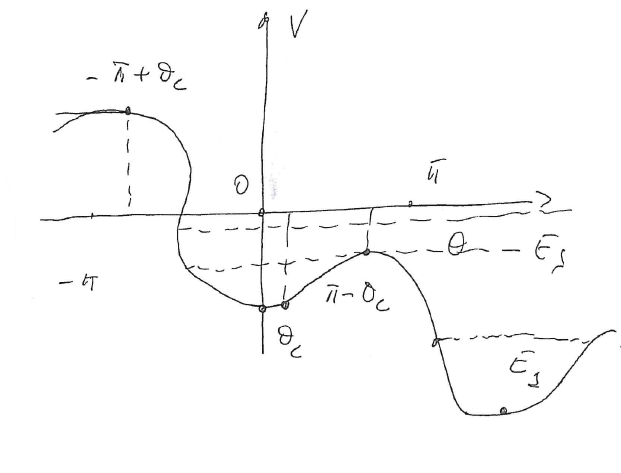
\includegraphics[width=0.6\linewidth]{pendolo-forzato}
	\caption{Rappresentazione grafica del potenziale del pendolo forzato nel caso \(f<k\).}
	\label{fig:pendolo-forzato}
\end{figure}
\FloatBarrier
L'equazione di Newton associata è
\[\ddot{\theta} = -k\sin\theta+f\]
che è periodica, nonostante la periodicità del potenziale sia rotta dalla presenza della forzante. Il ritratto di fase è invariante per traslazione, gli intorni dei punti critici restano simili a quelli del pendolo ma le separatrici sono molto diverse, perturbando un sistema le separatrici sono le prime a cambiare drasticamente, ciò è legato al fatto che le separatrici sono strettamente legate all'instabilità del sistema, cambiando di poco le condizioni del sistema il moto nell'intorno delle separatrici cambia notevolmente.
\begin{figure}[h!]
	\centering
	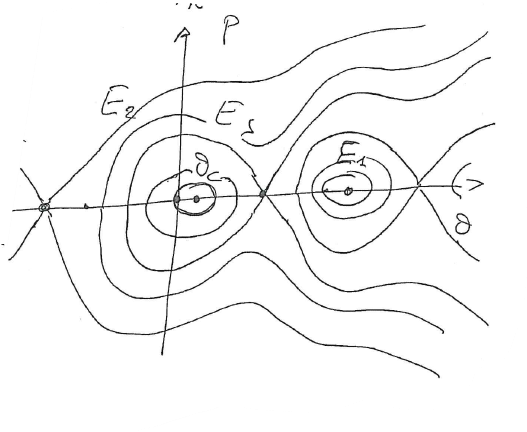
\includegraphics[width=0.6\linewidth]{pendolo-forzato-2}
	\caption{Ritratto di fase del pendolo forzato. La separatrice di un periodo è la curva all'infinito di quello precedente.}
	\label{fig:pendolo-forzato-2}
\end{figure}
\FloatBarrier
Approssimando a piccole oscillazioni nell'intorno di un punto ellittico siamo in grado di risolvere l'equazione differenziale ottenendo
\[\ddot{\theta} \simeq -k\theta+f\]
\[\theta (t) = c_1\cos(\sqrt{k} t) + c_2\sin(\sqrt{k} t) +\frac{f}{k}\]

\subsection{Risonanza parametrica e il problema dell'altalena}
Talvolta anche se un sistema vincolato è isolato e non agiscono forze esterne che fanno lavoro, si hanno comunque dei lavori interni al sistema dovuti alla variazione nel tempo del vincolo. dal principio dei lavori virtuali sappiamo che in un sistema isolato e vincolato, la somma dei lavori virtuali è nulla, sotto l'ipotesi che la reazione vincolare sia ortogonale al vincolo. Ad esempio, considerando una massa puntiforme attaccata all'estremità di un filo di lunghezza l (pendolo), e cioè vincolata a muoversi su una circonferenza di raggio l, sperimenta una forza vincolare in direzione radiale, ortogonale alla direzione (tangente alla circonferenza) del vincolo. Se però la lunghezza cambia nel tempo, il vincolo non sarà più circolare e dunque non si avrà sempre una reazione vincolare ortogonale ad esso: nel sistema vi sarà del lavoro dovuto a questo. Una situazione come quella appena illustrata è detta di risonanza parametrica in quanto il lavoro scaturisce dalla modifica di un parametro del sistema, in questo caso la lunghezza del filo. La parola "risonanza" indica il fatto che, se la variazione di lunghezza del pendolo è periodica, con una periodicità che rispetta alcune condizioni, il sistema entra il risonanza facendo aumentare esponenzialmente le oscillazioni. Analizzeremo una variante del problema illustrato che si rifà all'intuizione comune: il problema dell'altalena, che altro non è che il problema del pendolo di lunghezza variabile in modo costante a tratti. Quando ci sediamo su un'altalena siamo un pendolo ed il nostro centro di massa è la massa puntiforme attaccata all'estremità del pendolo (consideriamo la massa dell'altalena trascurabile); con la spinta iniziale abbiamo oscillazioni di piccola ampiezza che, senza attrito e senza forze esterne, sarebbero destinate a restare costanti nel tempo. Quando però muoviamo su e giù le gambe facciamo variare l'altezza del nostro centro di massa, ciò equivale a far variare la lunghezza del filo dell'altalena. Solitamente appare naturale stendere le gambe in salita e piegarle in discesa, in questo modo il pendolo avrà la stessa lunghezza \(l_{up}\) in tutte le salite ed \(l_{down}\) in tutte le discese. Concentrandosi su un singolo semiperiodo, e dunque su una salita o su una discesa, il moto è chiaramente quello di un'oscillatore armonico di velocità angolare \(\omega = \sqrt{\frac{g}{l}}\), avremo dunque due velocità angolari diverse $\omega_+$ per la salita e \(\omega_-\) per la discesa. Sappiamo il flusso di fase per i due semiperiodi up e down, che sono quelli di due oscillatori armonici, ma non conosciamo quello di un intero periodo. Per ottenerlo basta comporre i due flussi di fase dei due semiperiodi, visto che i flussi di fase godono delle proprietà di gruppo per la composizione
\begin{align*}
	\Phi_0^{2T}(x_0, \dot{x}_0) =  \Phi^{2T}_T\circ \Phi^{T}_0(x_0, \dot{x}_0) \equiv M^{2T}(x_0, \dot{x}_0)
\end{align*}
dove, per il vincolo che abbiamo, è conveniente adottare l'angolo dell'altalena con la verticale come coordinata e la velocità $v$ del centro di massa come momento. Per trovare la matrice \(M^{2T}\) basterebbe sviluppare il prodotto riga per colonna ma possiamo svolgere delle considerazioni: la composizione di flussi di fase deve conservare le aree, dunque \(det(M^{2T}) = 1\). Se diagonalizzo questa matrice, con la trasformazione P equivale ad un opportuno cambio di coordinate, avrò
\begin{align*}
	M^{2T} = P^{-1}
	\begin{pmatrix}
		\lambda_1&0\\
		0&\lambda_2
	\end{pmatrix} P\\
	det(M^{2T}) = 1 \Rightarrow\ \lambda_1\lambda_2 = 1
\end{align*}
dove si è usato il teorema di Binet e si è osservato che il determinane dell'identità è 1. Ma allora si hanno due opzioni: o gli autovalori sono uno il reciproco dell'altro, dunque
\[\lambda_1  = \frac{1}{\lambda_2}\]
oppure sono due complessi coniugati di modulo uno dunque
\[||\alpha+i\beta|| = 1\]
\[(\alpha+i\beta)(\alpha - i \beta) = \alpha^2+\beta^2 = ||\alpha + i \beta|| = 1\]
in questo caso potrei scrivere in forma esponenziale i due complessi, questi rappresentano una rotazione (identità di Eulero). Per vedere cosa accadrebbe se si continuassero ad oscillare le gambe come detto per un tempo pari ad n periodi, basterà comporre N volte la matrice \(M^{2T}\), ottenendo
\begin{align*}
	M^{2T} = P^{-1}
	\begin{pmatrix}
		e^{in\omega}&0\\
		0&e^{-in\omega}
	\end{pmatrix} P\\
\end{align*}
dunque la soluzione è stabile perché si hanno rotazioni di ampiezza costante. In questo caso dunque l'altalena continua ad oscillare con l'ampiezza iniziale, all'infinito.\\
Se però le soluzioni sono reali, una il reciproco dell'altra, dopo n periodi avremo
\begin{align*}
	M^{2T} = P^{-1}
	\begin{pmatrix}
		\lambda^n&0\\
		0&\lambda^{-n}
	\end{pmatrix} P\\
\end{align*}
avremo dunque una crescita esponenziale, l'altalena funziona! Le soluzioni si dicono stabili nel primo caso ed instabili nel secondo. Vogliamo capire in che condizioni abbiamo autovalori reali (per far funzionare l'altalena): guardo la traccia (si osservi che anche se non avessimo diagonalizzato i seguenti ragionamenti continuano ad essere validi in quanto la traccia è invariante per trasformazioni di similitudine). 
\[Tr(M^{2T}) = \lambda + \frac{1}{\lambda}\]
se \(\lambda = e^{i\omega}\) otteniamo
\[Tr(M^{2T}) = e^{i\omega} + e^{-i\omega} = cos(\omega)+i\sin\omega+\cos\omega - i \sin \omega = 2\cos\omega \leq 2\]
Se invece \(\lambda \in \mathbb{R}\) invece
\[Tr(M^{2T}) = \lambda + \frac{1}{\lambda} >2\]
ciò discende dalla condizione sul determinante. Dunque, per verificare la stabilità o l'instabilità del sistema, basterà calcolare il determinante di \(M^{2T}\) e vedere se è maggiore o minore di 2.
\newpage
\section{Formulazione Lagrangiana: vincoli e coordinate generalizzate}
La nascita della lagrangiana è avvenuta in rapporto allo studio dei vincoli e delle reazioni vincolari. Questo diverso punto di vista ci condurrà alle Equazioni di Eulero-Lagrange seguendo un percorso molto diverso da quello basato sul principio di minima azione, che vedremo nella prossima sezione. Nonostante la minor profondità e la minor valenza nell'ottica dello sviluppo di una teoria puramente analitica, questo punto di vista è estremamente istruttivo in quanto metterà in luce punti di vista diversi del formalismo lagrangiano.\\
La visione secondo cui ogni problema meccanico può essere risolto trovando le espressioni delle forze interne ed esterne di un sistema ed inserendole nel secondo principio della dinamica
\[m_i\ddot{x}_i = \sum_jF_{ji}+F_i^{(e)}\]
è riduttivo in quanto spesso accade che il sistema sia soggetto a vincoli.
\begin{definizione}[Vincolo]
	Un vincolo è una restrizione sui possibili valori di posizioni e le velocità che un sistema fisico può assumere. I vincoli che impongono restrizioni unicamnete sulle posizioni sono detti olonomi e sono esprimibili mediante una funzione delle coordinate del tipo
	\[F(q_1, ..., q_n) = 0\]
	tutti gli altri tipi di vincoli, cioè quelli che coinvolgono anche restrizioni sulle velocità, sono detti anolonomi.
\end{definizione}
\begin{esempio}[Vincoli olonomi]
	Il fatto che un sistema di particelle costituisca un corpo rigido è un vincolo esprimibile nella forma
	\[(x_i-x_j)^2-c_{ij}^2=0\]
	che equivale a dire che la distanza fra ogni coppia di particelle è costante.\\
	Un altro classico esempio di vincolo è la condizione che una particella debba muoversi su una superficie. Ad esempio, una particella che deve muoversi su una sfera di raggio r deve sottostare al vincolo
	\[x^2-a^2 = 0\]
\end{esempio}
La funzione mediante la quale è espresso il vincolo riduce i gradi di libertà del sistema, ad esempio se un punto materiale, che in generale può muoversi in uno spazio euclideo tridimensionale, è vincolato a muoversi su una superficie sferica, che è uno spazio bidimensionale, ha ridotto la dimensione dello spazio delle configurazioni di 1. 
\begin{osservazione}[Vincoli anolonomi]
	Per i vincoli anolonomi non è possibile ridurre i gradi di libertà, non esiste nessun procedimento generale per affrontare i problemi con questo tipo di vincoli; in generale bisogna trovare le equazioni differenziali che esprimono l'azione dei vincoli sul sistema. Nella meccanica classica tuttavia si assumono sempre vincoli olonomi, questa è una leggera limitazione dell'applicabilità della teoria a livello macroscopico perché i vincoli considerati solo fili o superfici che si approssimano come insetensibili e non deformabili (la deformazione porta con sè effetti dissipativi non conservativi che non possono essere espressi da vincoli olonomi). Tuttavia a livello microscopico non sono presenti effetti dissipativi, essendo questo un fenomeno emergente, dunque i vincoli possono sempre essere considerati olonomi; la fisica moderna è principalmente interessata al microscopico e in questo ambito i vincoli sono delle costruzioni matematiche per schematizzare comportamenti fisici. Da ora in poi dunque ci concentreremo unicamente su vincoli olonomi.
\end{osservazione}
\begin{definizione}[Vincoli reonomi e scleronomi]
	Un vincolo può cambiare nel tempo, ad esempio la superfiie su cui è vincolato il moto può deformarsi nel tempo o un filo può variare la sua lunghezza. Un vincolo dipendente dal tempo è detto reonomo, uno indipendente è detto scleronomo.
\end{definizione}
Nello spazio delle configurazioni un vincolo olonomo definisce una varietà, le configurazioni del sistema sono vincolate ad appartenere alla varietà. Nell'approccio Newtoniano, fondato su una struttura matematica euclidea (\(\mathbb{R}^3\) con la distanza euclidea) si tiene conto dei vincoli aggiungendo forze che impongono al sistema di restare sulla varietà (reazione vincolare). Geometricamente, ciò equivale ad immergere la varietà definita dal vincolo in \(\mathbb{R}^3\) ed aggiungere le razioni vincolari, ignote a priori. Questo processo è inutilmente farraginoso e lo scopo della formulazione lagrangiana sarà proprio quello di ripensare i vincoli. L'obiettivo che ci poniamo è quello di cambiare spazio (e metrica di conseguenza) in base al vincolo, ci proponiamo cioè di abbandonare l'a-priori di spazio \(\mathbb{R}^3\) considerando direttamente come spazio delle configurazioni la varietà definita dal vincolo.\\
I vincoli olonomi introducono due tipi di difficoltà nella soluzione di problemi meccanici:
\begin{itemize}
	\item Trovare le coordinate adattate al vincolo per ridurre i gradi di libertà
	\item Il vincolo esercita delle forze sul sistema per mantenerlo sul vincolo, queste forze non sono note e devono essere determinate per risolvere il problema.
\end{itemize}
Il primo problema si risolve effettuando un cambio di coordinate che riduca i gradi di libertà, queste coordinate dipenderanno unicamente dal vincolo e sono dette coordinate generalizzate o coordinate adattate al vincolo.
\subsection{Passare alle coordinate generalizzate}
Dato uno spazio vettoriale V, ci interessa definire il concetto di lunghezza o modulo di un vettore, per farlo dobbiamo costruire una struttura geometrica sullo spazio vettoriale V, cioè dobbiamo inserire il concetto di norma. La norma è una forma quadratica definita positiva a cui è associato il tensore G. Si osserva immediatamente che la G è un tensore di rango (0, 2)
\[|{x}| = x^jGx^i\]
poiché l'unico oggetto algebrico che moltiplicato per due oggetti controvarianti risulta in uno scalare è un tensore del tipo \(g_{ij}\), cioè di rango \((0, 2)\).\\
Sia V lo spazio delle configurazioni, allora il vettore posizione $\mathbf{x}\in V$ dunque le sue componenti sono controvarianti. Essendo in fisica classica il tempo uno scalare cioè un tensore di rango (0, 0), ed essendo la velocità la derivata della posizione sul tempo, anche la velocità sarà un vettore controvariante. Solo nel caso cartesiano la norma ha come tensore associato l'identità, cioé \(g_{ij} = \delta_{ij}\); il modulo quadro coincide così con la somma dei quadrati delle componenti cartesiane
\[|v|^2 = v^i \delta_{ij} v^j = (v^1)^2+(v^2)^2+(v^3)^2\]
Per passare in coordinate generalizzate, bisogna considerare una generica trasformazione cambio di coordinate da cartesiane \(x^i\) a generalizzate \(q^i\), questa trasformazione non è necessariamente lineare dunque non è sempre possibile associare una matrice alla trasformazione. Le componenti cartesiane saranno trasformate secondo una funzione vettoriale a valori vettoriali invertibile del tipo:
\[ x^i = x^i(q^j)\]
si osservi che abbiamo considerato, per semplicità, un cambio di coordinate non dipendente dal tempo ma in generale esistono anche quelli dipendenti dal tempo.
Differenziando otteniamo, usando la regola della catena
\[dx^i = \frac{\partial x^i}{\partial q^j}dq^j\]
possiamo vedere i
\[\mathbf{e}_j = \frac{\partial \mathbf{x}}{\partial q^j}\]
come i vettori dello spazio tangente allo spazio delle configurazioni
o equivalentemente gli
\[\frac{\partial x^i}{\partial q^j}\]
come gli elementi della matrice cambio di base:
\[A = a^i_j = \frac{\partial x^i}{\partial q^j}\]
che presenta sulle colonne i vettori della nuova base espressi nella vecchia, cioè, in forma vettoriale
\[e_j = \frac{\partial x}{\partial q^j}\]
dove x è un vettore espresso in coordinate cartesiane. Possiamo dunque riesprimere il cambio di coordinate, in forma vettoriale,come
\[dx =  dq^j e_j\]
dove dx è un vettore, cioè un oggetto invariante, non essendoci indici liberi. \\
Questo cambio di coordinate va a modificare anche la metrica. Per trovare la nuova metrica a partire dalla forma cartesiana ricaviamo il cambio di coordinate delle velocità derivando quest'ultima relazione e sostituendolo nell'espressione del modulo quadro della velocità in coordinate cartesiane
\[v^i = \frac{d}{dt}x^i =  \frac{d}{dt}(x^i(q^j)) = \frac{\partial x^i}{\partial q^j}\frac{d}{dt}q^j\]
\[|v|^2 = v^i \delta_{ij} v^j = \frac{\partial x^i}{\partial q^k}\frac{d}{dt}\dot{q}^k \delta_{ij}  \frac{\partial x^j}{\partial q^h}\frac{d}{dt}\dot{q}^h = 
\dot{q}^k\left( \frac{\partial x^i}{\partial q^k}\delta_{ij} \frac{\partial x^j}{\partial q^h}\right)\dot{q}^h=\]
\[\dot{q}^k\left( \frac{\partial x_j}{\partial q^k} \frac{\partial x^j}{\partial q^h}\right)\dot{q}^h = \dot{q}^kg_{kh}\dot{q}^h=|\dot{q}|^2\]
dunque la matrice metrica in coordinate generalizzate è 
\[g_{kh} = \frac{\partial x_j}{\partial q^k} \frac{\partial x^j}{\partial q^h} = a_k^i\delta_{ij}a^j_h = a_{jk}a^j_h =e_ke_h\]
che è un tensore di rango (2, 0) poiché j è un dummy index e l'operatore di derivata rispetto alle componenti controvarianti restituisce un vettore covariante.
\begin{osservazione}
	In questo contesto, abbiamo ricavato la metrica a partire dalla forma cartesiana effettuando una sostituzione perché, per comodità, abbiamo inizialmente derivato le proprietà della lagrangiana in forma cartesiana. Bisogna però rimarcare il fatto che le coordinate cartesiane non hanno alcuna priorità rispetto alle altre e che più propriamente si sarebbe potuti partire dal ricavare la lagrangiana in coordinate generalizzate, definendo la metrica come oggetto primitivo, legato allo spazio metrico considerato. La definizione della metrica dovrebbe quindi essere precedente rispetto alla scelta delle coordinate.
\end{osservazione}
Infine, possiamo esprimere la lunghezza di una curva \(\gamma\) come
\[L = \int_\gamma ds =\int_\gamma ||\dot{q}||dt = \int_\gamma \sqrt{\dot{q^j}g_{ji}\dot{q}^i}dt\]
\begin{esempio}[Coordinate polari]
	Per passare da coordinate cartesiane \(\mathbf{x} = (x, y)\) a coordinate polari \(\mathbf{q} = (r, \theta)\) sul piano si usa la seguente trasformazione
	\begin{align*}
		&\begin{cases}
			x = r\cos\theta\\
			y = r\sin\theta
		\end{cases}
	\end{align*}
	dunque la funzione vettoriale cambio di base è
	\[(x, y) = (x^1(r, \theta),\ x^2(r, \theta)) = (r\cos\theta, r\sin\theta)\]
	applicando la definizione
	\begin{align*}
		&g_{11} = (\frac{\partial r\cos\theta}{r},\ \frac{\partial r\sin\theta}{r})\cdot(\frac{\partial r\cos\theta}{r} \frac{\partial r\sin\theta}{r}) = \sin^2\theta+\cos^2\theta = 1\\
		&g_{12} = g_{21} =  (\frac{\partial r\cos\theta}{r}, \frac{\partial r\sin\theta}{\theta})\cdot(\frac{\partial r\cos\theta}{\theta}, \frac{\partial r\sin\theta}{r})= -r\sin\theta\cos\theta+r\cos\theta\sin\theta = 0 \\
		&g_{22} =  (\frac{\partial r\cos\theta}{\theta}, \frac{\partial r\sin\theta}{\theta})\cdot(\frac{\partial r\cos\theta}{\theta}, \frac{\partial r\sin\theta}{\theta}) =  r^2(sin^2\theta+cos^2\theta)= r^2
	\end{align*}
\end{esempio}
Si osservi come l'introduzione delle coordinate generalizzate faccia cadere la centralità di posizione e quantità di moto, che erano le coordinate privilegiate nella formulazione newtoniana, questo salto concettuale costituisce il primo punto di rottura introdotto dalla formulazione lagrangiana. Si noti che volendo seguire uno sviluppo totalmente formale e analitico bisognerebbe includere le coordinate generalizzate sin dall'inizio. Nell'approccio storico che stiamo seguendo ora tuttavia, partiamo dalla formulazione newtoniana per superarla (mettendoci nei panni di Lagrange). Il motivo che ha spinto Lagrange ad introdurre un nuovo formalismo è legato allo studio dei vincoli macroscopici. In generale un sistema formato da N particelle ha 3N gradi di libertà, se vi sono k equazioni vincolari i gradi di libertà si ridurranno a 3N-k.
\begin{esempio}[Coordinate adattate al vincolo per superficie sferica]
	In generale si dimostra che è sempre possibile trovare un opportuno cambio di coordinate che riduca il numero di gradi di libertà, queste sono dette coordinate adattate al vincolo.	Nel caso di vincolo sferico le coordinate adattate al vincolo sono quelle sferiche con r fissato, queste dipenderanno solamente da due variabili, ovvero i due angoli polare e azimutale, il raggio è fissato.
\end{esempio}
\begin{osservazione}[Coordinate generalizzate e vettori]
	Le coordinate generalizzate non possono sempre essere organizzate in vettori ortonormali come quelle cartesiane, ogni coordinata generalizzata può in generale avere diverse unità di misura e non esprime una componente della posizione come nel caso cartesiano.
\end{osservazione}
\subsection{Il principio di D'Alembert}
Superare la seconda difficoltà è più ostico e ci porta a voler formulare le leggi della dinamica in modo da non far apparire le forze vincolari, in questo modo si avrebbe a che fare solamente con forze note. 
\begin{definizione}[Spostamento virtuale infinitesimo]
	Si chiama spostamento virtuale infinitesimo di un sistema ogni spostamento corrispondente a una variazione arbitraria infinitesima delle coordinate compatibile con le forze e i vincoli imposti sul sistema all'istante dato t. L'aggettivo virtuale lo distingue dagli spostamenti reali, che avvengono in un intervallo di tempo durante il quale il vincolo e le forze possono cambiare. Indichiamo lo spostamento virtuale infinitesimo con "$\delta x$"
\end{definizione}
Se il sistema è all'equilibrio per definizione si ha che la forza risultante su ogni particella è nulla (\(F_i = 0\)). Ne segue che anche il prodotto scalare \(F_i\cdot \delta x_i = 0\), definendo il lavoro virtuale
\begin{definizione}[Lavoro virtuale infinitesimo]
	Il lavoro virtuale è dato dal prodotto scalare di una forza per uno spostamento virtuale infinitesimo.
\end{definizione}
segue che il lavoro virtuale infinitesimo è nullo, su ogni particella
\[\sum_i F_i\delta x_i = 0\]
La forza su una particella è formata da una componente dovuta alla reazione vincolare \(f_i\) ed una dovuta a forze attive \(F_i^{(a)}\)
\[\sum_i F_i^{(a)}\delta x_i + \sum_i  f_i\delta x_i = 0\]
Restringiamo la trattazione ai sistemi per i quali il lavoro virtuale delle forze vincolari è nullo. Osserviamo che questa condizione è ad esempio valida per il vincolo dei corpi rigidi ed è in generale valida se le forze vincolari sono ortogonali alla superficie definita dal vincolo: visto che gli spostamenti virtuali avvengono sempre tangenzialmente alla superficie avremo necessariamente lavoro virtuale nullo. Questa condizione è in generale valida per molti altri vincoli. Con questa restrizione stiamo ad esempio escludendo le forze d'attrito, che agiscono  nella stessa direzione del moto e che quindi fanno sempre lavoro. Questa limitazione non ha grande importanza in quanto l'attrito è un fenomeno emergente e a livello microscopico non è presente.	
L'espressione precedente dunque si riduce ad una forma detta
\begin{definizione}[Principio dei lavori virtuali]
	\[\sum_i F_i^{(a)}\delta x_i = 0\]
\end{definizione}
questa equazione soddisfa la necessità di eliminare le forze vincolari \(f_i\) ma è valida solamente per la statica, nel caso dinamico vale la seconda legge della dinamica
\[F_i  = \dot{p_i}\]
\[F_i-\dot{p}_i = 0\]
possiamo vedere questa nuova condizione è come se dicesse che le particelle del sistema sono in equilibrio sotto l'azione di una forza uguale alla forza attiva più una forza efficace opposta \(-\dot{p}_i\); ne segue che
\[\sum_i(F_i-\dot{p}_i)\delta x_i = 0\]
\[\sum_i(F^{(a)}_i-\dot{p}_i)\delta x_i + \sum_i f_i = 0\]
limitandoci, come prima, ai casi in cui la reazione vincolare è ortogonale alla superficie del vincolo, si ottiene una nuova forma del principio dei lavori virtuali:
\begin{teorema}[Principio di D'Alembert]
	\[\sum_i(F^{(a)}_i-\dot{p}_i)\delta x_i= 0\]
\end{teorema}
Passiamo ora alle coordinate generalizzate, come visto, (per semplicità non distingueremo covariante da controvariante):
\[ x_i = x_i(q_j, t)\]
nonostante abbiamo considerato un cambio di coordinate dipendente dal tempo, gli spostamenti virtuali, che avvengono in un istante di tempo fissato, comunque non dipenderebbero da esso; a rigore possiamo fare la distinzione tra spostamenti infinitesimi
\[d x_i = \frac{\partial x_i}{\partial q_j}d q_j + \frac{\partial x_i}{\partial t}dt\]
da cui discende la velocità
\[v_i = \frac{dx_i}{dt}= \frac{\partial x_i}{\partial q_j}\dot{q}_j + \frac{\partial x_i}{\partial t}\]
e spostamenti virtuali infinitesimi
\[\delta x_i =  \frac{\partial x_i}{\partial q_j}\delta q_j\]
esprimiamo anche il lavoro virtuale in coordinate generalizzate
\[\sum_i F_i\delta x_i = \sum_{i,j}F_i \frac{\partial x_i}{\partial q_j}d q_j = \sum_j Q_j d q_j\]
dove \(Q\) è detta forza generalizzata che in generale non ha le dimensioni di una forza ma notiamo che, moltiplicata per uno spostamento generalizzato, ha sempre le dimensioni di un lavoro (come notato in precedenza la coordinate generalizzate non hanno in generale le dimensioni di una lunghezza).\\
Vogliamo riscrivere il principio di D'Alembert in coordinate generalizzate, il primo pezzo è semplicemente la definizione di lavoro virtuale in coordinate generalizzate; il secondo pezzo richiede qualche manipolazione
\[\sum_i \dot{p}_i \delta x_i = \sum_i m_i \ddot{x}_i\delta x_i = \sum_{i, j} m_i \ddot{x}_i \frac{\partial x_i}{\partial q_j}\delta q_j\]
sfruttando la derivata di prodotto possiamo scrivere
\[\sum_{i, j} m_i \ddot{x}_i \frac{\partial x_i}{\partial q_j} = \sum_i \left[\frac{d}{dt}\left(m_i\dot{x}_i\frac{\partial x_i}{\partial q_j}\right) - m_i \dot{x}_i\frac{d}{dt}\left(\frac{\partial x_i}{\partial q_j}\right)\right]\]
nell'ultimo termine possiamo scambiare la derivata rispetto a t e \(q_j\) (non banale, sono due tipi di derivata diversi) poiché, in analogia a quanto fatto sopra, possiamo differenziare tutto \( \left(\frac{\partial x_i}{\partial q_j}\right) \) al posto di solamente \(x_i\), ottenendo
\[d\left(\frac{\partial x_i}{\partial q_j}\right) = \frac{\partial^2 x_i}{\partial q_j \partial q_k}dq_k + \frac{\partial^2 x_i}{\partial q_j \partial t}dt\]
da cui, dividendo per l'intervallo di tempo dt
\[\frac{d}{dt}\left(\frac{\partial x_i}{\partial q_j}\right) =  \frac{\partial^2 x_i}{\partial q_j \partial q_k}\dot{q}_k + \frac{\partial^2 x_i}{\partial q_j \partial t}\]
ma, ricordando l'espressione di \(v_i\) ottenuta in precedenza, risulta 
\[\frac{\partial}{\partial q_j} \frac{dx_i}{dt} = \frac{\partial }{\partial q_j}\left(\frac{\partial x_i}{\partial q_j}\dot{q}_j + \frac{\partial x_i}{\partial t}\right) =  \frac{\partial^2 x_i}{\partial q_j \partial q_k}\dot{q}_k + \frac{\partial^2 x_i}{\partial q_j \partial t}\]
\[\Rightarrow \frac{d}{dt}\left(\frac{\partial x_i}{\partial q_j}\right) = \frac{\partial}{\partial q_j} \frac{dx_i}{dt}\]
infine, scambiando le derivate e sostituendo la velocità otteniamo
\[\sum_i m_i \ddot{x}_i\frac{\partial x_i}{\partial q_j} = \sum_i \left[\frac{d}{dt}\left(m_i v_i\frac{\partial x_i}{\partial {q}_j}\right) - m_i v_i\left(\frac{\partial v_i}{\partial q_j}\right)\right]\]
inoltre, sempre dall'espressione di \(v_i\) si può ottenere la seguente relazione
\[\frac{\partial v_i}{\partial \dot{q}_j} = \frac{\partial x_i}{\partial q_j} + \frac{\partial}{\partial \dot{q}_i}\frac{\partial x_i}{\partial t} = \frac{\partial x_i}{\partial q_j}\]
poiché \(x_i\) non dipende dalla velocità. Dunque possiamo scrivere
\[\sum_i m_i \ddot{x}_i\frac{\partial x_i}{\partial q_j} = \sum_i \left[\frac{d}{dt}\left(m_i v_i\frac{\partial v_i}{\partial \dot{q}_j}\right) - m_i v_i\left(\frac{\partial v_i}{\partial q_j}\right)\right]\]
sfruttando la derivata di funzione composta ho che 
\[\frac{\partial v^2_i}{\partial \dot{q}_j} = 2v_i\frac{\partial v_i}{\partial \dot{q}_j} \]
\[\frac{\partial v^2_i}{\partial {q}_j} = 2v_i\frac{\partial v_i}{\partial {q}_j} \]
dunque posso raccogliere le derivate ed inserire quest'espressione nel principio di D'Alembert:
\[\sum_i \dot{p}_i\delta x_i = \sum_i m_i \ddot{x}_i\frac{\partial x_i}{\partial q_j}\delta q_j = \sum_j \left[\frac{d}{dt}\frac{\partial }{\partial \dot{q}_j}\left(\sum_i\frac{1}{2}m_i v^2_i\right) - \frac{\partial}{\partial q_j}\left(\sum_i\frac{1}{2}m_i v^2_i\right)\right]\delta q_j\]
riconoscendo l'energia cinetica in questa espressione sostituiamo
\[\sum_i \dot{p}_i\delta x_i = \sum_j \left[\frac{d}{dt}\frac{\partial T}{\partial \dot{q}_j} - \frac{\partial T}{\partial q_j}\right]\delta q_j\]
reinserendolo nel principio di D'Alembert
\[\sum_j \left[\frac{d}{dt}\frac{\partial T}{\partial \dot{q}_j} - \frac{\partial T}{\partial q_j}-Q_j\right]\delta q_j = 0\]
ma essendo i vincoli olonomi ed essendo le coordinate generalizzate scelte in modo da ridurre al minimo i gradi di libertà, essendo tutte indipendenti, l'espressione precedente è vera se e solo se
\[\frac{d}{dt}\frac{\partial T}{\partial \dot{q}_j} - \frac{\partial T}{\partial q_j} = Q_j\]
se assumiamo che le forze siano conservative, cosa sempre vera a livello microscopico, possiamo scrivere (assumendo che i potenziali non siano generalizzati) 
\[F_i = -\frac{\partial U}{\partial q_i}\]
\[Q_j = \sum_i  F_i \frac{\partial x_i}{\partial q_j} = -\sum_i\frac{\partial U}{\partial q_i}\frac{\partial x_i}{\partial q_j}\]
ma quest'ultima espressione è per definizione la derivata parziale della funzione \(U(x_1,\ ..., \ x_n)\) rispetto a \(q_j\). Infine otteniamo che, in sistemi conservativi, 
\[Q_j = -\frac{\partial U}{\partial q_j}\]
dunque, sostituendo nel principio di D'Alembert, posso portare U a primo membro, ricordando che non dipende dalle velocità per ipotesi ma solo dalle posizioni
\[\frac{d}{dt}\left(\frac{\partial (T-U)}{\partial \dot{q}_j}-\frac{\partial (T-U)}{\partial q_j}\right) = 0\]
ridefinendo \((T-U)\equiv \mathcal{L}\) abbiamo riottenuto le equazioni di Eulero Lagrange e l'espressione generale della lagrangiana.\\
Facendo cadere l'ipotesi che le forze siano conservative, possiamo ammettere che il potenziale dipenda da U(q, $\dot{q}$), in questo caso avremo potenziali generalizzati, che approfondiremo nella prossima sezione.
\subsection{Ottenere la reazione vincolare}
Consideriamo un vincolo olonomo del tipo
\[F(x) = 0\]
Avendo imposto che gli spostamenti virtuali sono sempre ortogonali al vincolo si ha
\[\frac{\partial F}{\partial x}\cdot \delta x = 0\]
Introducendo le coordinate adattate al vincolo la funzione \(F(x) = 0\) fissa la componente \(q^n\) dunque possiamo riscrivere la funzione del vincolo olonomo come
\[G(q^n) = 0\]
Ne segue che
\[\delta q^n = 0\]
Effettuando il cambio di variabili
\[\delta x^i = \frac{\partial x^j}{\partial q^i}\delta q^i\]
dove i va da 1 a n-1 mentre j va da 1 a n: abbiamo ridotto di 1 i d.o.f.\\
Sia f la reazione vincolare, cioè la forza esercitata dal vincolo per mantenere i corpi su di esso. Scrivo il secondo principio della dinamica (relazione vettoriale)
\[(ma-F^a-f)= 0\]
moltiplico per il versore della coordinata congelata, cioè mi concentro solo sulla n-esima componente
\[(ma-F^a)\frac{\partial x}{\partial q_n}= f\frac{\partial x}{\partial q_n}\]
osservando che la reazione vincolare f è parallela al versore \(\frac{\partial x}{\partial q_n}\) (poiché la reazione vincolare ha l'effetto di tenere fermo un corpo in questa direzione)
\[f\frac{\partial x}{\partial q_n} = f|\frac{\partial x}{\partial q_n}|\]
da questa relazione, come visto, si ottiene
\[\left(\frac{d}{dt}\frac{\partial}{\partial \dot{q}^nn}-\frac{\partial}{\partial q^n}\right)\mathcal{L} = f\frac{\partial x}{\partial q_n}\]
ma la coordinata \(q^n\) è fissa dunque la sua derivata temporale è nulla dunque la precedente relazione si riduce a
\[-\frac{\partial }{\partial q^n}\left(\frac{1}{2}\dot{q}^iG\dot{q}^j-\partial U\right) = f|\frac{\partial x}{\partial q_n}|\]
da cui si ottiene la reazione vincolare come
\[f = \frac{-\frac{\partial }{\partial q^n}\frac{1}{2}\dot{q}^iG\dot{q}^j+\frac{\partial U}{\partial q^n}}{|\frac{\partial x}{\partial q_n}|}\]
\newpage
\section{Formulazione Lagrangiana: il principio di minima azione}
Un modo equivalente, ma più astratto e più potente, di vedere la costruzione della lagrangiana si basa sul rompere definitivamente i legami con la formulazione Newtoniana sostituendo i principi della dinamica classica con un principio più generale e fondamentale.
\subsection{Principi variazionali eq equazione di Eulero-Lagrange}
\begin{definizione}[Funzionale reale]
	Sia X un insieme di funzioni, dominio del funzionale; un funzionale reale è definito come
	\[\mathcal{F}:X\rightarrow\mathbb{R}\]
	Si noti che il funzionale è una funzione a dimensione infinita essendo il suo dominio infinito dimensionale.
\end{definizione}
Nonostante la definizione di funzionale sia molto più generale, in fisica si considera il tipo più semplice e intuitivo di funzionale, cioè quello che associa un valore reale ad una funzione \(f\in X\) mediante l'operazione d'integrazione di una funzione F(f) fra due estremi fissati. Il funzionale di nostro interesse è dunque
\[\mathcal{F}[f] = \int_{a}^{b}F(x, f(x), f'(x))dx\]
Il calcolo delle variazioni è un'ambito della matematica che generalizza il problema dello studio dei punti estremali di una funzione al caso infinito dimensionale; per far ciò si fa uso dei funzionali e, in analogia con lo studio dei punti estremali di funzioni in spazi finito dimensionali, si definisce la derivata funzionale e la si pone nulla. Nel calcolo delle variazioni il dominio del funzionale svolge un ruolo cruciale perché questo definisce lo spazio entro il quale è possibile variare la funzione; il calcolo variazionale svolto su uno stesso funzionale offre risultati diversi se si cambia il dominio. Il dominio di interesse in fisica, per motivi che saranno presto chiari, è
\[X = \{f(t)\in C^{(2)}(t_a, t_b): f(t_a) = f_a, f(t_b) = f_b\}\]
si noti che abbiamo fissato gli estremi del dominio che, essendo costanti, non saranno affetti dalle variazioni.
\begin{definizione}[Derivata funzionale]
	Per poter definire la derivata avvalendosi del rapporto incrementale bisogna definire l'incremento di una funzione. Variare una funzione \(f\in X\) di una quantità \(\delta f\) vuol dire aggiungere una funzione \(\delta f\in X\) arbitrariamente piccola ad f. Definiamo
	\[\delta f = \varepsilon\phi\]
	con $\phi\in X$ ed $\varepsilon\in \mathbb{R}$ arbitrariamente piccola. Si noti che avendo fissato gli estremi del dominio, la variazione degli estremi è nulla
	\[\delta f(t_a) = \delta f(t_b) = 0\]
	 La derivata funzionale è dunque
	\[\frac{d\mathcal{F}}{df} = \lim_{\varepsilon\to 0}\frac{\mathcal{F}[f+\varepsilon\phi]-\mathcal{F}[f]}{\varepsilon}\]	
\end{definizione} 
\begin{definizione}[Estremale di un funzionale]
	\(f\in X\) è detto estremale di $\mathcal{F}$ se, variando f di una funzione \(\delta f\) piccola a piacere, restando dentro il dominio X, si altera il valore del funzionale di una quantità trascurabile rispetto alla variazione operata su f. In termini rigorosi possiamo dire che f è estremale per $\mathcal{F}$ se la derivata funzionale prima di $\mathcal{F}$ si annulla in f. Ovvero
	\[\mathcal{F}[f+\delta f] = \mathcal{F}[f]+o(||\delta f||)\] 
	Si noti che questa definizione è del tutto analoga a quella di punto estremale ben nota dall'analisi: un punto è estremale per una funzione se la derivata prima della funzione in quel punto si annulla, in questo caso lo sviluppo di Taylor di quella funzione attorno al punto è del tutto analoga a quella appena riportata.
\end{definizione}
\begin{teorema}[Equazioni di Eulero-Lagrange]
	Dato il funzionale
	\[\mathcal{F}[f] = \int_{t_a}^{t_b}F(t, f(t), f'(t))dt\]
	definito nel dominio
	\[X = \{f(t)\in C^{(2)}(t_a, t_b): f(t_a) = f_a, f(t_b) = f_b\}\]
	f(t) è estremale per $\mathcal{F}$ se e solo se soddisfa la relazione
	\[\left(\frac{\partial F}{\partial f}- \frac{d}{dt}\frac{\partial F}{\partial f'}\right) = 0\]
	detta Equazione di Eulero-Lagrange.
\end{teorema}
\begin{dimostrazione}
Calcoliamo dunque il funzionale di nostro interesse, definito mediante l'integrale, in \(f+\delta f\), sviluppiamo in serie di Taylor al primo ordine ed imponiamo che f sia estremale ponendo la derivata funzionale prima nulla. Sia \(f = f(t)\) ed \(f' = \frac{df}{dt}\) con t parametro reale.
\begin{align*}
	&\mathcal{F}[f+\delta f] = \int_{t_a}^{t_b}F(f+\delta f, f'+ \delta f', t)dt\simeq\\
	&\int_{t_a}^{t_b}\left(F(f, f', t)+<\left(\frac{\partial F}{\partial f}, \frac{\partial F}{\partial f'}, \frac{\partial F}{\partial t}\right), (\delta f, \delta f', 0)>\right)dt+o(||\delta f||)=\\
	&\int_{t_a}^{t_b}F(f, f', t)dt+\int_{t_a}^{t_b} \left(\frac{\partial F}{\partial f}\delta f+\frac{\partial F}{\partial f'}\delta f' \right)dt+o(||\delta f||)=\\
	&\mathcal{F}[f]+\int_{t_a}^{t_b} \left(\frac{\partial F}{\partial f}\delta f+\frac{\partial F}{\partial f'}\delta f' \right)dt+o(||\delta f||)
\end{align*}
Confrontando questa espressione con la definizione di estremale di funzionale, imponiamo che f sia estremale ponendo la variazione del funzionale nulla
\[\delta \mathcal{F} = \mathcal{F}[f+\delta f]-\mathcal{F}[f] = \int_{t_a}^{t_b} \left(\frac{\partial F}{\partial f}\delta f+\frac{\partial F}{\partial f'}\delta f' \right)dt= 0\]
Integriamo per parti il secondo addendo dentro l'integrale
\[\int_{t_a}^{t_b} \frac{\partial F}{\partial f'}\delta f'dt = \left[\frac{\partial F}{\partial f'}\delta f\right]^{t_b}_{t_a}-\int_{t_a}^{t_b}\left(\frac{d}{dt}\frac{\partial F}{\partial f'}\delta f\right)dt\]
ma per ipotesi, avendo definito il dominio fissando gli estremi di integrazione, si annulla il primo termine a secondo membro, ottenendo
\[\int_{t_a}^{t_b} \frac{\partial F}{\partial f'}\delta f'dt = -\int_{t_a}^{t_b}\left(\frac{d}{dt}\frac{\partial F}{\partial f'}\delta f\right)dt\]
Dunque
\[\delta \mathcal{F} = \int_{t_a}^{t_b} \left(\frac{\partial F}{\partial f}\delta f- \frac{d}{dt}\frac{\partial F}{\partial f'}\delta f\right)dt= \int_{t_a}^{t_b} \left(\frac{\partial F}{\partial f}- \frac{d}{dt}\frac{\partial F}{\partial f'}\right)\delta fdt = 0\]
Ma essendo $\delta f$ arbitrario per ipotesi sappiamo che per essere nullo l'integrale \(\forall \delta f\) è necessario che l'argomento dell'integrale sia nullo, da cui
\[\left(\frac{\partial F}{\partial f}- \frac{d}{dt}\frac{\partial F}{\partial f'}\right) = 0\]
Si noti che \(f(t)\) e $\dot{f}(t)$ sono in generale vettori n-dimensionali dunque questa espressione in realtà racchiude n equazioni differenziali del secondo ordine, che richiedono 2n condizioni iniziali per essere univocamente risolte, sono ad esempio necessari i valori per \(t=0\) delle \(f(t)\) e \(f'(t)\).
\end{dimostrazione}
L'applicazione fisica consiste semplicemente nel postulare che le traiettorie fisiche sono tali da rendere minimo un funzionale, detto azione
\begin{assioma}[Principio di minima azione]
	I corpi descrivono traiettorie tali da minimizzare il funzionale d'azione
	\[\mathcal{S}[x(t)]=\int_{t_a}^{t_b}\mathcal{L}(x(t), \dot{x}(t), t)dt\]
	dove S è il funzionale d'azione, di dimensioni di un'energia per tempo, ed $\mathcal{L}$ è la lagrangiana, funzione caratteristica del sistema fisico considerato e che definisce la fisica di questo, con le dimensioni di un energia.
\end{assioma}
\begin{osservazione}
	Questo assioma sostituisce il secondo assioma della dinamica.
\end{osservazione}
Ne segue che le variabili f(t) sono le traiettorie q(t) dove q è una coordinata generalizzata, \(x_a\) e \(x_b\) sono dunque gli estremi di una traiettoria e l'integrale è operato lungo la traiettoria.

\subsection{Le proprietà della lagrangiana della particella libera}
Il problema ora è determinare l'espressione di \(F(x, \dot{x}, t) \), è chiaro che avendo già visto la formulazione lagrangiana in termini di vincoli e coordinate generalizzate sappiamo che F sarà la lagrangiana poiché questa occupa il posto di F nelle equazioni di Eulero-Lagrange (chiameremo d'ora in poi F "lagrangiana"), tuttavia per costruire una meccanica in modo puramente analitica a partire dal principio di minima azione dobbiamo essere in grado di ottenere la stessa forma senza prendere ulteriori assiomi.\\
Cominciamo con l'evidenziare un fatto implicitamente già visto nella dimostrazione precedente
\begin{teorema}
	La lagrangiana di un sistema è definita a meno di una derivata totale rispetto al tempo
			\[\frac{dA}{dt}\]
		Inoltre la moltiplicazione della lagrangiana per una costante non ha effetto sulle equazioni del moto. 
\end{teorema}
\begin{dimostrazione}
	Da un punto di vista matematico la lagrangiana è definita indirettamente dal principio di minima azione, dove compare all'interno della variazione di un integrale che ha gli estremi fissati. Se consideriamo 
	\[\mathcal{L}' = \mathcal{L}+\frac{dA}{dt}\]
	\[\mathcal{S}'[x(t)]=\int_{t_a}^{t_b}\mathcal{L'}(x(t), \dot{x}(t), t)dt = \int_{t_a}^{t_b}\left(\mathcal{L}(x(t), \dot{x}(t), t)+\frac{dA}{dt}\right)dt=\]
	\[\mathcal{S}[x(t)]+\int_{t_a}^{t_b}dA= \mathcal{S}[x(t)]+\left(A(t_b)-A(t_a)\right)\]
	dove gli addendi sono costanti perché gli estremi d'integrazione sono fissi. Variando $\mathcal{S}$ e $\mathcal{S'}$, si ottiene evidentemente lo stesso principio variazionale, perché la variazione degli estremi è nulla
	\[\delta\mathcal{S}'=\delta \mathcal{S}\]
	abbiamo ottenuto lo stesso principio variazionale.\\
	Da un punto di vista fisico, la lagrangiana definisce la fisica del sistema, ovvero l'evoluzione dello stato del sistema nel tempo; se due espressioni diverse di $\mathcal{L}$ portano alle stesse equazioni del moto, a seguito dell'applicazione dell'operatore di Lagrange, allora sono la stessa lagrangiana.\\
	Infine, consideriamo la moltiplicazione per una costante
	\[\mathcal{L}' = a\mathcal{L}\]
	otteniamo lo stesso principio variazionale riscalato per una costante
	\[\delta\mathcal{S}'=a\delta S\]
	ma, passando alle equazioni di Eulero-Lagrange
	\[\left(\frac{\partial}{\partial x}- \frac{d}{dt}\frac{\partial}{\partial \dot{x}}\right)a\mathcal{L} = 0\]
	\[\Rightarrow\ \left(\frac{\partial}{\partial x}- \frac{d}{dt}\frac{\partial}{\partial \dot{x}}\right)\mathcal{L}= 0\]
	che porta alle stesse equazioni del moto della lagrangiana non moltiplicata per la costante a.
\end{dimostrazione}
Determiniamo dunque la forma della lagrangiana, inizialmente per una particella libera in un sistema di riferimento inerziale usando coordinate cartesiane per semplicità (il passaggio a coordinate generalizzate è immediato, come visto nella sezione precedente).
\begin{definizione}[omogeneità ed isotropia]
	Un sistema è definito omogeneo se ogni sua parte presenta le medesime caratteristiche fisiche delle altre.\\
	Un sistema è definito isotropo se presenta le medesime caratteristiche fisiche in tutte le direzioni.
\end{definizione}
 Nei S.R.I. per definizione spazio e tempo sono omogenei ed lo spazio è anche isotropo. Per definizione di omogeneità, la lagrangiana, che definisce la fisica del sistema, non può dipendere esplicitamente dalla coordinata q e dal tempo, perché questo implicherebbe che a seconda del punto dell'universo o dell'istante in cui ci si trova le leggi della fisica sono diverse, ma questo va conto l'assioma di semplicità. La lagrangiana dipenderà unicamente dalla velocità. Essendo lo spazio isotropo la lagrangiana non può dipendere dalla direzione della velocità ma solo dal suo modulo, dunque la lagrangiana dipenderà dal quadrato della velocità.
\[\mathcal{L} = \mathcal{L}(\dot{x}^2)\]
Ma se la lagrangiana del corpo libero non dipende da q allora
\[\frac{\partial \mathcal{L}}{\partial x} = 0\]
l'equazione di Eulero Lagrange diventa
\[\frac{d}{dt}\frac{\partial\mathcal{L}}{\partial \dot{x}} = 0\]
ma allora 
\[\frac{\partial\mathcal{L}}{\partial \dot{x}} = cost.\]
ed avendo detto che la lagrangiana dipende unicamente dalla velocità ne deduciamo che il moto di una particella libera, per il principio di minima azione, è tale da mantenere la velocità costante nel tempo.\\
Se un S.R.I. K' si muove a velocità costante infinitesima $\varepsilon$ rispetto al S.R.I. K, per le trasformazioni di galileo si ha
\[\dot{x}' = \dot{x}+\varepsilon\]
Per l'assioma di relatività le leggi della fisica devono restare della stessa forma nei due S.R.I., dunque le equazioni del moto devono essere le stesse, dunque \(\mathcal{L}'\) può differire da $\mathcal{L}$ al più per una derivata totale rispetto al tempo
\[\mathcal{L}' = \mathcal{L}(\dot{x}'^2) = \mathcal{L}(\dot{x}'^2) = \mathcal{L}(\dot{x}^2+(\varepsilon^2+2\dot{x}\varepsilon))\]
essendo \(\varepsilon\) infinitesima possiamo sviluppare in serie di Taylor attorno a \(\dot{x}^2\) trascurando le potenze superiori alla prima di $\varepsilon$
\[\mathcal{L}(\dot{x}'^2) \simeq \mathcal{L}(\dot{x}^2) + \frac{\partial\mathcal{L}}{\partial\dot{x}^2}(\dot{x}'^2-\dot{x}^2)+o(||\dot{x}'^2-\dot{x}||) =\]\[ \mathcal{L}(\dot{x}^2) + \frac{\partial\mathcal{L}}{\partial\dot{x}^2}(2\dot{x}\varepsilon+\varepsilon^2)+o(||\dot{x}'^2-\dot{x}||) \simeq\]
\[ \mathcal{L}(\dot{x}^2) + \frac{\partial\mathcal{L}}{\partial\dot{x}^2}(2\dot{x}\varepsilon)+o(\varepsilon)\]
Perché le equazioni di Lagrange mantengano la stessa forma cambiando S.R.I. è necessario che il secondo addendo del secondo membro scompaia applicando l'operatore di Lagrange, ciò è possibile solo se questo è una derivata totale rispetto al tempo, cioè deve verificarsi
\[\frac{\partial\mathcal{L}}{\partial\dot{x}^2} = a = cost.\]
infatti in questo modo
\[\frac{d}{dt}(2a\varepsilon x) = 2a\varepsilon \dot{x}\]
che equivale a dire che la lagrangiana deve dipendere da $\dot{x}^2$ secondo la relazione 
\[\mathcal{L} = a \dot{x}^2\]
questa forma rispetta il principio di relatività ma è stata dedotta per una velocità relativa fra S.R.I. infinitesima. Da quanto dimostrato è immediatamente deducibile la validità anche per velocità relative finite $v$
\[\mathcal{L}' = a\dot{x}'^2 = a (\dot{x}+v)^2= a\dot{x}^2+2av\dot{x}+av^2= L+\frac{d}{dt}(2av x+av^2t)\]
Dove il secondo addendo dell'ultimo membro è una derivata totale rispetto al tempo (la costante a è la costante moltiplicativa del teorema precedente). Ritroviamo facilmente il fatto che a non influenza le equazioni del moto applicando l'operatore di Lagrange. Questa costante viene solitamente identificata con \(m/2\) dunque la lagrangiana della particella libera è
\[\mathcal{L} = \frac{m}{2}\dot{x}^2\]
Se però a è una costante moltiplicativa arbitraria, e noi la interpretiamo come la massa, senza altre restrizioni sarebbe per principio possibile moltiplicare due diverse lagrangiane per costanti arbitrarie diverse \(a_1\) e \(a_2\). Questa libertà va contro la nostra comune concezione di massa, secondo cui la massa è una qualità intrinseca del corpo e non è possibile cambiarla a piacere. Effettivamente ci sono delle restrizioni non banali sulla scelta della costante moltiplicativa, che legittima la sua interpretazione in termini di massa.
\begin{osservazione}[Additività della lagrangiana]
	Un'altro fatto fondamentale relativo alla lagrangiana, che costituisce la sua enorme potenza in fisica è la sua additività: se un sistema fisico è composto di due parti A e B, non interagenti fra loro (ad esempio se sufficientemente lontane), di lagrangiana rispettivamente \(\mathcal{L}_A\) ed \(\mathcal{L}_B\), allora la lagrangiana dell'intero sistema è la somma delle lagrangiane. Se invece le due parti fossero in interazione bisognerebbe tener conto dell'energia potenziale d'interazione fra le parti, che dipende dalla distanza fra esse e dalla loro posizione; l'ipotesi presa è dunque necessaria. 
\end{osservazione}
\begin{teorema}
	Dall'additività della lagrangiana discende la limitazione sui possibili valori che le costanti moltiplicative \(a_i\): la costante moltiplicativa deve essere la stessa per tutti i sistemi fisici. Inoltre la costante deve essere positiva.
	
\end{teorema}
\begin{dimostrazione}
	Consideriamo un sistema formato da due particelle libere non interagenti. La lagrangiana del sistema formato dalla somma delle due particelle è per additività
	\[\mathcal{L}_{1+2} = \mathcal{L}_1+\mathcal{L}_2\]
	Per assurdo, se si potessero moltiplicare le due lagrangiane per costanti diverse, senza cambiare la fisica del sistema, si avrebbe
	\[\mathcal{L}_1\rightarrow a_1 \mathcal{L}_1\]
	\[\mathcal{L}_2\rightarrow a_2 \mathcal{L}_2\]
	la lagrangiana \(\mathcal{L}'_{1+2}\), ottenuta dalla somma di queste due nuove lagrangiane, deve produrre la stessa fisica di quella precedente, dunque deve essere uguale a \(\mathcal{L}_{1+2}\) a meno di una derivata totale rispetto al tempo e una costante moltiplicativa. Tuttavia, per l'additività 
	\[\mathcal{L}'_{1+2} = a_1\mathcal{L}_1+a_2\mathcal{L}_2\]
	la moltiplicazione per due costanti arbitrarie diverse ha cambiato la fisica del sistema! Questo è assurdo. Ne segue che le due costanti moltiplicative devono essere uguali, in questo caso infatti
	\[\mathcal{L}_{1+2} = a\mathcal{L}_1+a\mathcal{L}_2 = a(\mathcal{L}_{1+2})\] 
	che produce le stesse equazioni del moto se vi si applica l'operatore lagrangiano. \\
	Infine, visto che per principio l'azione deve essere minima, se moltiplicassimo la lagrangiana per una costante negativa (il che equivarrebbe ad avere una massa negativa), essendo la velocità al quadrato sempre positiva, e potendo assumere valori arbitrariamente grandi in meccanica classica, si avrebbe che il funzionale d'azione può assumere valori arbitrariamente piccoli, da cui segue che non possiede un minimo. L'esistenza di una massa negativa romperebbe il principio di minima azione. 
\end{dimostrazione}
\begin{osservazione}
	La libertà di moltiplicare tutti i sistemi fisici isolati per una stessa costante arbitraria equivale alla libertà di scelta dell'unità di misura della massa: se ad esempio esprimiamo la massa in chilogrammi abbiamo che la lagrangiana di un sistema formato da particelle libere non interagenti è del tipo
	\[\mathcal{L} = \sum_i\mathcal{L}_i = \sum_i\frac{1}{2}m_i\dot{x}_i^2\]
	se moltiplichiamo tutti i sistemi isolati formati dalle singole particelle per la stessa costante \(a = 10^{3}\) 
	\[\mathcal{L}10^{3} = \sum_i\mathcal{L}_i10^{3} = \sum_i\frac{(m_i10^{3})}{2}\dot{x}_i^2 = \sum_i\frac{m'_i}{2}\dot{x}_i^2\]
	non stiamo facendo altro che esprimere la massa in grammi.
\end{osservazione}
\subsection{Energia e lagrangiana}\label{subsec:energia-lagra}
La lagrangiana della particella libera non dipende esplicitamente dal tempo, questo è intuitivamente vero poiché uno degli assiomi di semplicità imponeva che le leggi della fisica non varino con il tempo. Scriviamo la derivata della lagrangiana nel tempo
\[\frac{d\mathcal{L}}{dt} = \frac{\partial \mathcal{L}}{\partial q_i}\dot{q}_i+ \frac{\partial \mathcal{L}}{\partial \dot{q}_i}\ddot{q}_i\]
Uso le equazioni di Lagrange per ottenere una derivata di prodotto
\[\frac{d\mathcal{L}}{dt} = \frac{d}{dt}\frac{\partial \mathcal{L}}{\partial \dot{q}_i}\dot{q}_i+ \frac{\partial \mathcal{L}}{\partial \dot{q}_i}\ddot{q}_i=\frac{d}{dt}\left(\frac{\partial\mathcal{L}}{d\dot{q}_i}\dot{q}_i\right)\]
\[\frac{d}{dt}\left(\frac{\partial\mathcal{L}}{d\dot{q}_i}\dot{q}_i-\mathcal{L}\right)=0\]
\[\Rightarrow E = \frac{\partial\mathcal{L}}{d\dot{q}_i}\dot{q}_i-\mathcal{L}=cost.\]
Questa è la definizione di energia usata in meccanica analitica che, se calcolata sostituendo la lagrangiana della particella libera in forma cartesiana, coincide con la definizione di energia ottenuta dalla conservazione delle aree. Vedremo in seguito come la conservazione dell'energia discende da una simmetria del tempo, come evidenziato dal teorema di N\"{o}ther.
\subsection{L'interazione fra particelle: potenziali e potenziali generalizzati}
Da ora in poi si adotterà la notazione indiciale. Se una grandezza non è contrassegnata da indici è un vettore, una matrice o uno scalare, ciò sarà chiaro dal contesto.\\
Si osserva che particelle a distanza finita interagiscono fra loro e modificano reciprocamente le traiettorie; la lagrangiana di un sistema di particelle, per far sì che il principio di minima azione resti valido, e cioè per far sì che le equazioni del moto siano ancora da esso deducibili, deve tener conto di questa interazione. Consideriamo un sistema formato da n particelle interagenti fra loro ma non con l'esterno, questo tipo di sistema è detto isolato. Si osserva sperimentalmente che l'interazione fra queste particelle è descrivibile aggiungendo alla lagrangiana una funzione a valori scalari U in generale dipendente dalla posizione e dalle sue derivate rispetto al tempo (il fatto che sia scalare è necessario perché la lagrangiana deve essere scalare in modo da essere invariante).
\[\mathcal{L} = \frac{m}{2}\dot{x}^i\dot{x}_i-U\]
dove \(-U\) è la funzione che descrive l'interazione. Il fatto che sia negativa è frutto della convenzione. Chiameremo il primo termine della lagrangiana energia cinetica ed il secondo energia potenziale.
\begin{osservazione}
	Si noti che il fatto che è possibile tener conto dell'interazione fra le particelle con una funzione uguale per tutti i sistemi di riferimento inerziali con una forma che non varia nel tempo e nello spazio (la funzione dipende dal tempo e dallo spazio ma la sua forma funzionale non cambia) equivale all'assioma di semplicità.
\end{osservazione}
Applicando l'operatore lagrangiano alla forma generale della lagrangiana di una particella otteniamo
\[\left(\frac{d}{dt}\frac{\partial}{\partial \dot{x}^i}-\frac{\partial}{\partial x^i}\right)\left(\frac{m}{2}\dot{x}^i\dot{x}_i-U\right) = 0\]
\begin{align}\label{eq:pot-gen}
	m\frac{d\dot{x}^i}{dt} = \frac{d}{dt}\frac{\partial U}{\partial \dot{x}^i}-\frac{\partial U}{\partial x^i}
\end{align}
Se il potenziale dipende solo dalla posizione \((U=U(x^i))\) si ottiene la medesima definizione di forza che si aveva in fisica newtoniana 
\[m\frac{d\dot{x}_i}{dt} = -\frac{\partial U}{\partial x^i}=F_i\]
in questo modo si riottiene il secondo principio della dinamica, che è stato dedotto dal principio di minima azione, che lo ha sostituito.\\
Tuttavia il potenziale può a priori dipendere, oltre che dalla posizione, dalla velocità e da derivate successive della posizione (questa eventualità non è tenuta in considerazione dalla fisica newtoniana), in generale si ha
\[F_i = \frac{d}{dt}\frac{\partial U}{\partial \dot{x}^i}-\frac{\partial U}{\partial x^i}\]
Osserviamo che vi sono delle restrizioni sulle grandezze da cui può dipendere il potenziale. Dalla definizione di forza, sappiamo che questa è la causa dell'accelerazione, dunque non può dipendere da essa, altrimenti si cadrebbe in un circolo vizioso. Ne segue che il potenziale non può dipendere dall'accelerazione o da derivate superiori alla prima della posizione perché in questo caso, applicando l'operatore lagrangiano, o si annullerebbe o, se dipendesse dal prodotto di velocità per accelerazione o posizione per accelerazione, risulterebbe una forza dipendente da un'accelerazione, il che è assurdo. Inoltre il potenziale non può dipendere da potenze superiori alla prima della velocità perché in questo caso il primo termine dell'operatore lagrangiano produrrebbe una forza dipendente dall'accelerazione. Nulla vieta però che il potenziale dipenda linearmente dalla velocità; se U dipendesse solamente dalla velocità, non vi potrebbe dipendere linearmente perché in questo caso U sarebbe un vettore: l'unica possibilità rilevante è che il potenziale dipenda linearmente dalla velocità moltiplicata per potenze della posizione. In questo caso entrambi i termini della (\ref{eq:pot-gen}) sono in generale non nulli e non dipendono dall'accelerazione.
\begin{definizione}[Potenziale generalizzato]
	Un potenziale \( U = U(x^i, \dot{x}^i)\) dipendente sia dalla posizione che dalla velocità è detto potenziale generalizzato, in contrapposizione ai potenziali dipendenti unicamente dalla posizione, detti semplicemente potenziali. \\
	Osserviamo che U è una funzione a valori scalari, la velocità ha componenti controvarianti dunque un potenziale generalizzato deve dipendere, linearmente dalla velocità moltiplicata ad una funzione \(A_j(x)\) covariante, funzione delle posizioni. Ne segue che un potenziale generalizzato ha forma
	\[U(\dot{x}^j, x^j) = k\dot{x}^jA_j(x)\]
	(in alcuni passaggi, per leggerezza di notazione, tralasceremo la k per poi reintrodurla)
\end{definizione}
\begin{osservazione}[Conservatività]
	Condizione necessaria e sufficiente affinché una forza sia conservativa è che lungo ogni percorso chiuso fa lavoro nullo. Questo avviene se la forza è esprimibile come gradiente di un potenziale dipendente unicamente dalla posizione: in questo modo, per il teorema fondamentale del calcolo, l'integrale del lavoro dipenderà unicamente dai punti di inizio e fine percorso e dunque sarà sempre nullo in percorsi chiusi (in cui inizio e fine coincidono). Se la forza discende da un potenziale generalizzato, è sicuramente impossibile esprimere la forza come un gradiente dipendente dalla posizione perché vi è una dipendenza dalla velocità oltre che dalla posizione. Ne segue che tutte le forze derivanti da potenziali generalizzati sono non conservative.  
\end{osservazione}
L'introduzione dei potenziali generalizzati e di \(A_j\) è stata del tutto formale, ci chiediamo che tipo di forze possano scaturire da potenziali generalizzati, e se queste esistono in natura. Applichiamo l'operatore lagrangiano. Ipotizziamo dapprima che il potenziale generalizzato non dipenda esplicitamente dal tempo
\[\left(\frac{d}{dt}\frac{\partial}{\partial \dot{x}^i}-\frac{\partial}{\partial x^i}\right)\dot{x}^jA_j(x) = F_i\]
\[\frac{d}{dt}A_i(x)-\dot{x}^j\frac{\partial}{\partial x^i}A_j(x)= F_i\]
\[\frac{\partial A_i}{\partial x^j}\dot{x}^j-\dot{x}^j\frac{\partial A_j}{\partial x^i}= F_i\]
dove questa espressione è valida solo se A non dipende da non dipende esplicitamente dal tempo
\[\left(\frac{\partial A_i}{\partial x^j}-\frac{\partial A_j}{\partial x^i}\right)\dot{x}^j=F_i\]
Il termine fra parentesi ricorda l'espressione indiciale del rotore. Per dare un significato fisico al potenziale generalizzato svolgiamo alcuni passaggi sfruttando la regola del BAC-CAB (in forma indiciale il prodotto scalare fra due vettori deve essere contratto: stesso indice uno covariante e uno controvariante)
\[\dot{x}\times\left(\frac{\partial}{\partial x}\times A\right) = \frac{\partial }{\partial x^i}(\dot{x}^jA_j)-\left(\dot{x}^j\frac{\partial}{\partial x^j}\right)A_i= \left(\frac{\partial A_j}{\partial x^i}-\frac{\partial A_i}{\partial x^j}\right)\dot{x}^j = -F_i\]
Da cui segue
\begin{align}\label{eq:f-gen}
	F = k\dot{x}\times (rotA)=k\left(\frac{\partial A_j}{\partial x^i}-\frac{\partial A_i}{\partial x^j}\right)\dot{x}^j = \left(\frac{d}{dt}\frac{\partial}{\partial \dot{x}}-\frac{\partial}{\partial x}\right)(-k(\dot{x}A)) 
\end{align}
\[U(x, \dot{x}) = -k(\dot{x}A)\]
\begin{osservazione}[Potenziali generalizzati e lavoro]
	Consideriamo la potenza di una forza scaturente da un potenziale generalizzato
	\[W = F_i\dot{x}^i = k\left(\frac{\partial A_i}{\partial x^j}-\frac{\partial A_j}{\partial x^i}\right)\dot{x}^j\dot{x}^i\]
	Si noti che il membro tra parentesi è antisimmetrico (cambia segno se scambio gli indici) mentre quello fuori dalle parentesi è simmetrico (non cambia segno se scambio gli indici), inoltre tutti gli indici sono muti, essendo la potenza uno scalare; la somma di tutti i termini deve essere nulla. Ne segue che la potenza erogata è nulla, dunque forze scaturenti da potenziali generalizzati non dipendenti dal tempo non fanno lavoro.\\
	Questo non sarebbe vero se A dipendesse esplicitamente dal tempo, infatti dalla definizione di forza (tenendo conto dei potenziali generalizzati) si avrebbe
	\[F_i = -k\frac{d}{dt}A_i(x, t)+k\dot{x}^j\frac{\partial}{\partial x^i}A_j(x, t) =\]
	\[-k\frac{\partial A_i}{\partial t} -k\frac{\partial A_i}{\partial x^j}\frac{\partial x^j}{\partial t}+k\frac{\partial A_j}{\partial x^i}\dot{x}^j = -k\frac{\partial A_i}{\partial t} -k\left(\frac{\partial A_i}{x^j}-\frac{\partial A_j}{x^i}\right)\dot{x}^j\]
	\[W = -k\frac{\partial A}{\partial t}\dot{x}^i\neq 0\]
	dunque una forza scaturente da un potenziale generalizzato fa lavoro solo se dipende esplicitamente dal tempo e il termine che genera lavoro è del tipo appena ottenuto.
\end{osservazione}
\begin{osservazione}[Potenziali generalizzati ed energia]
	L'energia è un'integrale primo del moto proprio di tutte le lagrangiane non dipendenti dal tempo e scaturente dalla simmetria d'omogeneità del tempo, come mostrato dai teoremi di  N\"{o}ther. Da questo teorema si ricava la definizione di energia come
	\[E \equiv \dot{x}^j\frac{\partial \mathcal{L}}{\partial \dot{x}^j}-\mathcal{L}\]
	Se la lagrangiana non presenta potenziali generalizzati l'energia è
	\[E = \dot{x}^j\frac{\partial }{\partial \dot{x}^j}(\frac{m}{2}\dot{x}^i\dot{x}_i)-\frac{m}{2}\dot{x}^i\dot{x}_i+U(x) = T + U\]
	se sono presenti potenziali generalizzati non dipendenti dal tempo, come osservato in precedenza non si hanno ulteriori contributi all'energia perché 
	\[\dot{x}^j\frac{\partial k\dot{x}^iA_i}{\partial \dot{x}^j}-k\dot{x}^iA_i = 0\]
	se invece il potenziale generalizzato dipende dal tempo l'espressione dell'energia resta sempre la stessa ma la lagrangiana dipenderà dal tempo, dunque la simmetria temporale è rotta e l'energia non è più un integrale del moto. L'informazione sul potenziale generalizzato si perde nell'energia ma è presente nell'espressione dei momenti 
	\[p_i = \frac{\partial \mathcal{L}}{\partial \dot{x}^i} = \frac{\partial T}{\partial \dot{x}^i}+\frac{\partial (k\dot{x}^jA_j)}{\partial \dot{x}^i} = \frac{\partial T}{\partial \dot{x}^i} + kA_i\]
	Lo spazio delle fasi è modificato, dunque la fisica del sistema è diversa. 
\end{osservazione}
Vediamo ora due esempi fisici di forze scaturenti da potenziali generalizzati
\begin{esempio}[Campo elettromagnetico]
	Definendo
	\[rotA\equiv B\]
	(si noti che in questo modo esistono diversi A il cui rotore può essere uguale a B)
	\[k \equiv \frac{q}{c}\]
	 otteniamo dalla (\ref{eq:f-gen}) la forza di Lorentz
	\[F = \frac{q}{c}\dot{x}\times B\]
	Possiamo immediatamente dedurre una delle equazioni di Maxwell senza alcun riferimento all'esperienza: applichiamo la divergenza al campo magnetico
	\[div B = div(rotA) = 0\]
	Sappiamo sperimentalmente che il campo magnetico non fa lavoro ma abbiamo osservato che se A dipende esplicitamente dal tempo, e dunque B dipende dal tempo, allora si ha lavoro, com'è possibile? Il termine di forza che fa lavoro è, come osservato
	\[F_i = -\frac{q}{c}\frac{\partial A_i}{\partial t}\]
	il responsabile del lavoro non è il campo magnetico ma il campo elettrico, che definiamo come
	\[E_i \equiv -\frac{\partial A_i}{\partial t}\]
	Calcolando il rotore del campo elettrico otteniamo un'altra delle equazioni di Maxwell
	\[rot E = -\frac{\partial }{\partial t}rotA = -\frac{\partial B}{\partial t} \]
\end{esempio}
\begin{esempio}[Forza di Coriolis]
	Sia K un S.R.I. e K' un S.R. rotante, sia X un vettore posizione rispetto K e x rispetto K'. Per passare da K' a K bisogna effettuare una rotazione degli assi di K', variabile nel tempo R(t)
	\[X = R(t)x\]
	\[X^i = r^i_jx^j\]
	derivando rispetto al tempo 
	\[\dot{X} = \dot{R}x+R\dot{x}\]	
	\[\dot{X}^i = \dot{r}^i_kx^k+r^i_j\dot{x}^j\]	
	il membro a sinistra rappresenta la velocità assoluta, cioè la velocità del vettore rispetto al S.R.I., nel membro a destra invece abbiamo la velocità assoluta espressa in termini di coordinate del sistema rotante; questa è composta di due parti: la prima è detta velocità di trascinamento, cioè la velocità dovuta alla rotazione del S.R. vista dal S.R.I., la seconda è la velocità del vettore x relativa al suo S.R. K', vista da K.\\
	La matrice di rotazione è ortogonale, dunque l'inversa coincide con la trasposta, per passare dalle grandezze espresse rispetto al S.R.I. a quello rotante basta applicare la trasposta ad ambo i membri
	applico la trasposta ad ambo i membri alla relazione delle velocità per ricavare la velocità rispetto K'
	\[R^T\dot{X} = R^T\dot{R}x+R^TR\dot{x} = R^T\dot{R}x+\dot{x}\]
	Osservo che derivando la matrice \(R^TR = I\) ottengo
	\[\frac{d}{dt}(R^TR) = \dot{R}^TR+R^T\dot{R} = 0\]
	\[(R^T\dot{R})^T+R^T\dot{R} = 0\]
	\[(R^T\dot{R})^T= -R^T\dot{R} \]
	che dimostra che la matrice \(\dot{R}R^T\) è antisimmetrica. In notazione indiciale
	\[\frac{d}{dt}(r^j_ir^i_j) = \dot{r}^k_ir^i_j+\dot{r}^i_kr^j_i = 0\]
	\[\dot{r}^i_kr^j_i = -(\dot{r}^k_ir^i_j)\]
	Possiamo ridefinire
	\[(\dot{R}R^T)\equiv\Omega\]
	\[\dot{r}^i_kr^j_i\equiv\omega^j_k\]
	Le matrici antisimmetriche 3x3 hanno tre gradi di libertà (la condizione di antisimmetria ne fissa 6 su 9) e sono del tipo
	\begin{align*}
		\omega^j_k = 
		\begin{pmatrix}
			0&-\omega^1_2&\omega^1_3\\
			\omega^2_1&0&-\omega^2_3\\
			-\omega^3_1&\omega^3_2&0
		\end{pmatrix}
	\end{align*}
	Si dimostra che è sempre possibile associarvi la terna, che ribattezziamo
	\[\omega = (\omega^2_3, \omega^1_3, \omega^2_1) \equiv (\omega^1, \omega^2, \omega^3)\]
	\[\Omega \leftrightarrow \omega\]
	e che, data una matrice cambio di base B, questa terna trasforma con la seguente relazione
	\[\tilde{\omega}^i = det(B) b^i_j\omega^j \]
	e che dunque è, per definizione, uno pseudovettore (ecco giustificato il motivo per cui la terna è stata ribattezzata usando componenti controvarianti). Si dimostra inoltre che vale la seguente proprietà
	\begin{align*}
			\Omega x = 
			\begin{pmatrix}
				0&-\omega^3&\omega^2\\
			\omega^3&0&-\omega^1\\
			-\omega^2&\omega^1&0
			\end{pmatrix}
			\begin{pmatrix}
				x^1\\
				x^2\\
				x^3
			\end{pmatrix}=
			\begin{pmatrix}
				-x^2\omega^3+x^3\omega^2\\
				-x^3\omega^1+x^1\omega^3\\
				-x^1\omega^2+x^2\omega^1
			\end{pmatrix}=
			 \omega\times x
	\end{align*}
	Interpretiamo il vettore associato a questa matrice antisimmetrica come la velocità angolare. Per approfondimenti su questi passaggi si veda (\ref{ap:rotazioni})\\
	da ciò segue che la velocità assoluta espressa rispetto al S.R. rotante è esprimibile come 
	\[R^T\dot{X} = (\omega\times x)+ \dot{x}\]
	la legge generale di trasformazione della derivata temporale passando da un S.R.I. ad uno rotante è dunque
	\begin{align}\label{eq:derivata-rotante}
	&\left(\frac{d}{dt}\right)_{S.R.I.} = \left(\frac{d}{dt}\right)_{S.R.}+ (\omega\times \cdot)
	\end{align}
	Possiamo dunque scrivere la lagrangiana di una particella in un sistema rotante, l'energia cinetica è definita come una forma quadratica della velocità vista da un S.R.I., dunque
	\[\mathcal{L} = T = \frac{m}{2}\left(\frac{dx}{dt}\right)_{S.R.I.}^2 = \frac{m}{2}\left[\left(\frac{dx}{dt}\right)_{S.R.}+ (\omega\times x)\right]^2 =\]
	\[ \frac{m}{2} \dot{x}^2 + \frac{m}{2}(\omega\times x)^2+m\dot{x}(\omega\times x)\]
	Dove il primo termine a secondo membro è l'energia cinetica relativa al sistema rotante, il secondo è un potenziale centrifugo, l'ultimo termine è un potenziale generalizzato: dipende linearmente dalla velocità $\dot{x}$ moltiplicata per un vettore, in cui figura la posizione, questo è il cosiddetto potenziale generalizzato di Coriolis ed è il potenziale apparente dovuto alla rotazione del S.R. 
	\begin{osservazione}
		Un cambio di coordinate può far sorgere nuovi potenziali apparenti, questo è vero anche per il potenziale magnetico che è dovuto ad una rotazione 4-D (trasformazione di Lorentz nello spazio di Minkowski), se una carica comincia a ruotare genera campo magnetico. 
	\end{osservazione}
	Per come abbiamo definito i potenziali generalizzati risulta
	\[U(x, \dot{x}) = -k\dot{x}^iA_i =-m\dot{x}(\omega\times x)\]
	Applichiamo l'operatore di lagrange per trovare la forza generata da questo potenziale:
	\[\left(\frac{d}{dt}\frac{\partial}{\partial\dot{x}}-\frac{\partial}{\partial x}\right) \left(-m\dot{x}(\omega \times x)\right) = \frac{d}{dt}(-m(\omega \times x))+m(\dot{x}\times \omega) \]
	dove nell'ultimo passaggio ho ciclato i termini presenti nel prodotto scalare per il prodotto vettoriale in quanto questo rappresenta un volume, il risultato non cambia a meno dei segni a cui devo fare attenzione. Infine, derivando ed invertendo i termini del prodotto vettoriale
	\[F= -2m(\omega\times\dot{x})\]
\end{esempio}
\begin{esempio}[Analogia Potenziale magnetico-Coriolis]
Nel caso del campo magnetico non siamo riusciti a determinare un'espressione di A, che risulta ancora un oggetto introdotto formalmente. Ricaviamone l'espressione per analogia con il potenziale di Coriolis, in particolare osserviamo che dall'espressione del potenziale e della forza
\[-m(\omega\times{x})\dot{x}\leftrightarrow\ -\frac{q}{c}A\dot{x} \]
\[-2m(\omega\times\dot{x})\leftrightarrow -\frac{q}{c}(B\times\dot{x})\]
notiamo che B è l'analogo di $\omega$, che k=$\frac{q}{c}$ per il campo magnetico e \(m\) per Coriolis. Inoltre, nel caso di Coriolis, nel passare dal potenziale alla forza compare un coefficiente \(2\) al numeratore, per mantenere l'analogia, questo termine deve essere
\[A = \frac{1}{2}(B\times x)\] 
dunque il potenziale magnetico generalizzato deve essere
\[U(x, \dot{x}) = -\frac{q}{2c}(B\times x)\dot{x}\]
se \(B = B_0\hat{z}\), questa espressione si riduce a 
\[U = -\frac{q}{2c}(-B_0y\dot{x}+B_0x\dot{y})\]
\'E importante ricordare che la definizione di A non è univoca e che l'espressione ricavata con questa analogia non è l'unica possibile, ad esempio, si consideri un campo magnetico costante lungo le x: \(B = (B_0, 0, 0)\), chiaramente sarà valido, per analogia
\[A = \frac{1}{2}(0, -B_0 z, B_0 y)\]
il cui rotore risolta proprio \(B = (B_0, 0, 0)\), tuttavia, si consideri
\[A = (0, -B_0 z, 0)\]
anche il suo rotore è \(B = (B_0, 0, 0)\). Ciò non sarebbe stato vero se B fosse stato costante ed unicamente diretto lungo l'asse z! Bisognerà scegliere la rappresentazione più conveniente.
\end{esempio}
\begin{osservazione}
	Il fatto che l'energia potenziale dipende dalle posizioni delle particelle implica che lo spostamento di una particella si ripercuote istantaneamente su tutte le altre particelle. Questo è equivalente a dire che l'informazione si propaga a velocità infinita. Questo è sperimentalmente falso ed è un risultato sbagliato che segue dall'assioma sbagliato della fisica classica secondo cui il tempo è assoluto. Da questo segue l'assioma di relatività di Galilei che non tiene conto del cambiamento del tempo fra sistemi di riferimento inerziali e da questo segue che la luce, e quindi l'informazione, viaggiano a velocità infinita. La relatività ristretta elimina l'assioma di assolutezza del tempo e lo sostituisce con l'assioma della costanza della velocità della luce, che, avendo un valore finito, impedisce che l'informazione possa viaggiare a velocità infinita. 
\end{osservazione}
\begin{osservazione}[Isotropia del tempo]
	Dalla definizione di S.R.I. discende l'omogeneità di spazio e tempo e l'isotropia dello spazio per le leggi fisiche, non si è parlato però dell'isotropia del tempo: le leggi della fisica sono le stesse se il tempo va verso il futuro o verso il passato? Questo fatto dipende dalla forma delle leggi fisiche, cioè dalla forma della lagrangiana da cui discendono. Dalla forma generale della lagrangiana appena vista, si nota che, non essendoci dipendenza esplicita dal tempo, le leggi della fisica hanno la medesima forma per \(t\) o per \(-t\). Questo vuol dire in termini pratici che se si fa un filmato dell'evoluzione di un sistema di particelle, non è possibile distinguere se il video stia andando al contrario o meno. Si dice per questo che i sistemi fisici godono di reversibilità temporale (time-reversibility), se è possibile un qualsiasi moto, è possibile anche l'inverso. In termini geometrici, se l'evoluzione temporale di una particella è una curva sullo spazio delle fasi, le leggi della fisica non distinguono i due orientamenti possibili della curva. 
\end{osservazione}
\begin{esercizio}[Pendolo di Foucault]
	Si consideri un punto materiale vincolato da una molla a muoversi su un piano tangente ad una sfera (la terra) che ruota di velocità angolare costante (molto piccola) attorno l'asse z di un S.R.I. con centro nel centro della sfera. Il punto in cui è fissato la molla, sulla sfera, è l'origine di un S.R. rotante solidale alla sfera, con asse z' in direzione del raggio congiungente il centro della sfera con il punto in cui è fissata la molla, il punto materiale si muove sul piano x'y'. Possiamo calcolare l'energia cinetica rispetto al S.R. rotante, rispetto ad esso la velocità angolare cambia nel tempo ma l'energia cinetica deve essere calcolata da un S.R.I. dunque non è importante l'istante che scegliamo, scegliamo quello in cui ha una forma facile: sia \(\omega\) la velocità angolare nel S.R.I. e $\omega'$ nel S.R., scegliamo l'istante in cui $\omega '$ si trova sul piano z'y'
	\[\omega ' = (0, \omega\sin\alpha, \omega\cos\alpha)\]
	per scrivere l'energia cinetica dobbiamo esprimere la velocità della particella rispetto al S.R.I. con la nota relazione
	\[\dot{x} = \dot{x'}+(\omega '\times x') = (\dot{x}', \dot{y}')+\omega \times (z'\sin\alpha-y'\cos\alpha, x'\cos\alpha, -x'\sin\alpha)\]
	una via corretta per risolvere il problema sarebbe quella di sviluppare queste espressioni ma è evidentemente un conto molto lungo, dunque sostituiamo direttamente nell'energia cinetica
	\[T = \frac{m}{2}\dot{x}^2 = \frac{m}{2}(\dot{x}'+(\omega '\times x') )^2 =\frac{m}{2}\dot{x}'^2+\frac{m}{2}(\omega' \times x')^2+m\dot{x}'(\omega' \times x') \]
	dove il secondo termine è centrifugo mentre il terzo è il potenziale di Coriolis, visto che $\omega$ è molto piccolo e nel termine centrifugo compare al quadrato, possiamo trascurare questo termine. Da ora in poi dovremo essere coerenti nel trascurare termini di ordine superiore al primo di \(\omega '\). Sviluppando l'espressione osservando che visto che il moto è vincolato al piano tangente della sfera si ha \(\dot{x}' = (\dot{x}', \dot{y}', 0)\), otteniamo
	\begin{align*}
		(\dot{x}', \dot{y}', 0)\cdot
		det
		\begin{pmatrix}
			\hat{i}&\hat{j}&\hat{k}\\
			0&\omega\sin\alpha&\omega\cos\alpha\\
			x'&y'&0
		\end{pmatrix}=\omega\cos\alpha(x'\dot{y}'-\dot{x}'y')
	\end{align*}
	\[T = \frac{m}{2}(\dot{x}'^2+\dot{y}'^2) +m\omega \cos\alpha(x'\dot{y}'-\dot{x}'y')+o(\omega')\]
	Possiamo ora scrivere la lagrangiana tenendo conto del potenziale elastico
	\[\mathcal{L} = \frac{m}{2}(\dot{x}'^2+\dot{y}'^2) +m\omega \cos\alpha(x'\dot{y}'-\dot{x}'y')-\frac{k}{2}(x'^2+y'^2)\]
	Osserviamo che la lagrangiana è quadratica: applicando l'operatore di Lagrange otteniamo equazioni del moto lineari, il moto avrà solamente due gradi di libertà perché la molla è un vincolo olonomo, abbiamo due equazioni (equazioni del moto di Lagrange) in due incognite (x', y'), il sistema è integrabile.\\
	Un modo elegante di risolvere il problema è quello di usare coordinate complesse (z sarà la nuova coordinata e non più l'asse z)
	\begin{align*}
		z = x'+iy'\\
		\overline{z} = x'-iy'
	\end{align*}
	osservando che
	\[\dot{z}\overline{z} = (\dot{x}'+i\dot{y}')(x'-iy') = (\dot{x}x+y\dot{y})+i(\dot{y}x-\dot{x}y)\]
	ne prendiamo la parte immaginaria per sostituirlo nella lagrangiana
	\[Im(\dot{z}\overline{z}) = \frac{\dot{z}\overline{z}-\overline{\dot{z}\overline{z}}}{2i} = -\frac{i}{2}(\dot{z}\overline{z}-z\dot{\overline{z}})\]
	rimettendo insieme i pezzi
	\[\mathcal{L}(z, \overline{z}) = \frac{m}{2}\dot{z}\dot{\overline{z}}-\frac{i}{2}m\omega\cos\alpha(\dot{z}\overline{z}-z\dot{\overline{z}})-\frac{k}{2}z\overline{z}\]
	l'operazione complesso coniugato può entrare nella derivata, se scrivo le equazioni di Lagrange rispetto lee mie coordinate ottengo due equazioni che sono l'una la complessa coniugata dell'altra. Si osservi che l'operazione svolta è stata quella di passare da un sistema di due equazioni in due incognite reale ad un'equazione in un'incognita complessa, ciò non è strano in quanto i complessi sono isomorfi ad \(\mathbb{R}^2\). Considero una sola equazione: 
	\[\left(\frac{d}{dt}\frac{\partial}{\partial \dot{\overline{z}}}-\frac{\partial}{\partial \overline{z}}\right)\left(\frac{m}{2}\dot{z}\dot{\overline{z}}-\frac{i}{2}m\omega\cos\alpha(\dot{z}\overline{z}-z\dot{\overline{z}})-\frac{k}{2}z\overline{z}\right) = 0\]
	\[\ddot{z}+2i\omega\cos\alpha \dot{z}+\nu^2 z = 0\]
	dove
	\[\nu= \sqrt{\frac{k}{m}}\]
	la soluzione dell'equazione differenziale si ottiene imponendo una soluzione del tipo \(e^{\lambda t}\), ricaviamo così il polinomio caratteristico
	\[\lambda^2+2i\omega\cos\alpha\lambda \omega^2 + \nu^2 = 0\]
	da cui ricaviamo $\lambda$ 
	\[\lambda = -i\omega\cos\alpha\pm\sqrt{-\nu^2-\omega^2\cos^2\alpha}\]
	ma abbiamo trascurato le potenze di $\omega$ dunque
	\[\lambda = -i\omega\cos\alpha\pm\sqrt{-\nu^2} = -i\omega\cos\alpha\pm i\nu\]
	la soluzione è data da
	\[z(t) = c_1 e^{t (-i\omega\cos\alpha+ i\nu)} + c_2 e^{t (-i\omega\cos\alpha- i\nu)} = \]
	\[e^{-i\omega\cos\alpha t}\left[c_1e^{i\nu t} + c_2 e^{- i \nu t}\right]\]
	dove le costanti \(z_0 = c_1 + c_2 = x'+ i y'\) contengono le informazioni sulle condizioni iniziali di x' e y'.\\
	osserviamo che questa è la soluzione dell'oscillatore armonico moltiplicata per un fasore: il pendolo di Foucault è un'oscillatore armonico (molla o pendolo sono matematicamente uguali) che oscilla e contemporaneamente ruota, la rotazione è dovuta alla velocità angolare terrestre: in questo modo si dimostra la rotazione della terra attorno al suo asse  d è possibile calcolarne la velocità angolare.
\end{esercizio}
\begin{osservazione}
	Da un S.R. non inerziale è possibile, essendo solidali ad esso, misurare caratteristiche proprie del S.R.; ciò non è possibile per S.R.I., la cui unica caratteristica è la velocità costante, che non è misurabile essendo solidali al S.R.I. 
\end{osservazione}
\begin{esercizio}[Sfera con campo magnetico]
Si consideri un punto materiale di massa m e carica q vincolato ad una superficie sferica, consideriamo un S.R.I. con origine nel centro della sfera, un campo magnetico costante d'intensità \(B_0\) è diretto lungo l'asse z. Le coordinate adattate sono chiaramente quelle sferiche, l'energia cinetica in queste coordinate è
\[T = \frac{m}{2}(r^2\dot{\theta}^2+r^2\dot{\phi}^2\sin^2\theta)\]
con r fissato.Il potenziale, di tipo generalizzato, è come prima
\[U = -kA\dot{x}= -\frac{q}{2c}(B \times x)\dot{x}\]
sviluppo in prodotto vettoriale 
\[(B \times x) = (0, 0, B_0)\times (x, y, z) = (-y, x, 0)\]
questa è proprio la direzione \(\hat{\phi}\), cioè tangente alla sfera su piani paralleli ad xy. Infatti
\[e_\phi = \frac{\partial x}{\partial \phi} = \frac{\partial }{\partial \phi}(r\sin\theta\cos\phi, r\sin\theta\sin\phi, r\cos\theta) = (-y, x, 0)\] 
questo è ovvio se si conosce la fenomenologia del campo magnetico. Infine, moltiplico scalarmente per la velocità e ottengo
\[U = -\frac{B_0 q}{2c}\dot{\phi}r^2\sin^2\theta\]
\[\mathcal{L} = \frac{m}{2}(r^2\dot{\theta}^2+r^2\dot{\phi}^2\sin^2\theta)+\frac{B_0 q}{2c}\dot{\phi}r^2\sin^2\theta\]
osservo che \(\phi\) è ciclico, me lo aspettavo per la simmetria di rotazione attorno l'asse z, calcolo in momento associato
\[p_\phi = r^2m\dot{\phi\sin^2\theta+\frac{q B_0}{2c}\sin^2\theta}\]
L'altro integrale del moto è l'energia perché la lagrangiana è indipendente dal tempo, lo calcolo con la definizione essendoci un potenziale generalizzato
\[ E = \frac{m}{2}(r^2\dot{\phi}^2+r^2\dot{\phi}^2\sin^2\theta)= \]
\[ = \frac{m}{2}r^2\dot{\phi}^2 + \frac{p_\phi^2}{2mr^2\sin^2\theta}+\frac{mr^2}{2}\left(\frac{q B_0}{2c mr^2}\right)^2\sin^2\theta\]
quest'ultima è un'equazione differenziale nella sola incognita $\theta$, integrabile.
\end{esercizio}


\newpage
\section{Il teorema di N\"{o}ther}
In questa sezione useremo da principio coordinate generalizzate, data la generalità di questo teorema.
\begin{definizione}[Simmetria di un sistema fisico]
	Sia X lo spazio delle configurazioni di un sistema fisico e q un suo vettore, che per un sistema formato da una singola particella che si muove in uno spazio tridimensionale è del tipo
	\[q = (q_1,q_2,q_3)\]
	Un flusso $\Psi^{(\alpha)}(q)$, automorfismo definito sullo spazio delle configurazioni, ad un parametro reale (in questo caso \(\alpha\))
	\[\Psi:X\times\mathbb{R}\rightarrow X\]
	che sia un gruppo abeliano rispetto all'operazione di composizione e tale che la lagrangiana sia invariante rispetto all'applicazione di tale trasformazione
	\[\mathcal{L}(q, \dot{q}) = \mathcal{L}(\Psi^{(\alpha)}(q), \frac{d}{dt}\Psi^{(\alpha)}(q))\]
	è detta simmetria del sistema fisico.\\
	Il campo vettoriale generatore è definito come
	\[a(q_0)\equiv \frac{\partial}{\partial \alpha}|_{\alpha = 0}\Psi(q_0)^\alpha\]
	e, analogamente a quanto visto per il flusso di fase, dall'ipotesi di gruppo discende
	\[a(q) = \frac{d}{d\alpha}|_{\alpha = 0}\Psi^\alpha(q)=\frac{dq}{d\alpha}(\alpha)\]
	Visto che la fisica del sistema è determinata dalla forma della lagrangiana, $\Psi$ è una trasformazione delle coordinate del sistema che non modifica la fisica del sistema.
\end{definizione}
\begin{osservazione}
	Si faccia attenzione al fatto che una simmetria è un flusso (definizione \ref{def:flusso}) e non un flusso di fase: è definita sullo spazio delle configurazioni e non sullo spazio delle fasi. Una simmetria è dunque un flusso di fase che non dipende dai momenti e che conserva la lagrangiana è una simmetria. 
\end{osservazione}
\begin{definizione}[Momento associato ad una coordinata]
	Sia $\mathcal{L}$ una lagrangiana e \(q\) una coordinata generalizzata, definiamo momento associato alla coordinata \[p_q = \frac{\partial \mathcal{L}}{\partial \dot{q}}\]
	Si noti che se la lagrangiana non dipende dalla coordinata, cioè la coordinata è ciclica, allora il momento ad essa associato è un'integrale primo del moto. Ciò risulta chiaro applicando l'operatore di Lagrange usando l'ipotesi $\mathcal{L}=\mathcal{L}(\dot{q})$ indipendente da \(q\)
	\[\left(\frac{d}{dt}\frac{\partial}{\partial \dot{q}}-\frac{\partial}{\partial q}\right)\mathcal{L}(\dot{q}) = \frac{d}{dt}\frac{\partial}{\partial \dot{q}} = \frac{dp_q}{dt} = 0\] 
	 Si osservi inoltre che il momento associato ad una coordinata è covariante mentre la coordinata è controvariante: il loro prodotto risulta in un'invariante.
\end{definizione}
\begin{osservazione}
	Essendo la lagrangiana definita a meno di una derivata totale rispetto al tempo, anche il momento non risulta univocamente definito
	\[p_i = \frac{\partial \mathcal{L}}{\partial \dot{q}^i}\]
	\[p'_i = \frac{\partial \mathcal{L}}{\partial \dot{q}^i}+\frac{\partial}{\partial \dot{q}^i}\frac{dF}{dt} =  \frac{\partial \mathcal{L}}{\partial \dot{q}^i} +  \frac{\partial F}{\partial q^i} \]
	dunque se q è ciclica per $\mathcal{L}$ non lo è per forza anche per $\mathcal{L'}$.
\end{osservazione}
\begin{teorema}[Teorema di  N\"{o}ther]
	Le simmetrie di un sistema fisico stanno in rapporto biunivoco con gli integrali primi del moto. La relazione che lega la simmetria \(\Psi\) all'integrale primo del moto I è
	\[I = p_qa(q)\]
\end{teorema}
\begin{osservazione}[Importanza dell'ipotesi di gruppo]
	La richiesta che la simmetria abbia la proprietà di essere un gruppo è fondamentale per poterla mettere in relazione con il campo vettoriale e quindi costruire le equazioni differenziali. Il modo in cui avviene l'associazione è identico a quello visto per i flussi di fase, cambia solo l'insieme su cui è definita la trasformazione. In particolare, come per i flussi di fase, la simmetria diventa l'identità per $\alpha= 0$
\end{osservazione}
\begin{dimostrazione}
	Essendo $\Psi^{(\alpha)}(q)$ una simmetria allora per definizione, \(\forall \alpha\):
	\[\mathcal{L}(q, \dot{q}) = \mathcal{L}(\Psi^{(\alpha)}(q), \frac{d}{dt}\Psi^{(\alpha)}(q))\]
	essendo la lagrangiana sempre uguale per qualsiasi valore di $\alpha$ allora
	\[\frac{d}{d\alpha}\mathcal{L}(\Psi^{(\alpha)}(q), \frac{d}{dt}\Psi^{(\alpha)}(q)) = 0\]
	sviluppando la derivata totale con la regola della catena
	\[\frac{d\mathcal{L}}{d\alpha}(\Psi^{(\alpha)}(q), \frac{d}{dt}\Psi^{(\alpha)}(q)) = \frac{\partial \mathcal{L}}{\partial q}\frac{\partial \Psi^{(\alpha)}(q)}{\partial \alpha}+\frac{\partial \mathcal{L}}{\partial \dot{q}}\frac{\partial}{\partial \alpha}\frac{d}{dt}\Psi^{(\alpha)}(q) = 0\]	
	sviluppiamo in serie di Taylor rispetto ad $\alpha$ attorno al punto $\alpha = 0$ al primo ordine. $\alpha$ compare solo nelle derivate delle simmetrie dunque sviluppiamo queste e sostituiamo
	\[\Psi^{(\alpha)}(q)\simeq \Psi^{(0)}(q) + \frac{d}{d\alpha}|_{\alpha=0}\Psi^{(\alpha)}(q)\alpha+o(\alpha) = q + a(q)\alpha+o(\alpha)\]
	\[\frac{d}{dt}\Psi^{(\alpha)}(q)\simeq \dot{q}+ \alpha \frac{d}{dt}a(q)+o(\alpha)\]
	dove ho usato il fatto che per \(\alpha = 0\) la simmetria è l'identità e la definizione di campo vettoriale associato alla simmetria. Sostituendo
	\[\frac{\partial\mathcal{L}}{\partial \alpha} \simeq \frac{\partial\mathcal{L}}{\partial q}a(x)+\frac{\partial \mathcal{L}}{\partial \dot{q}}\frac{d}{dt}a(x)=0\]	
	Sostituendo le equazioni del moto
	\[\left(\frac{d}{dt}\frac{\partial}{\partial \dot{q}}-\frac{\partial}{\partial q}\right)\mathcal{L} = 0\]
	\[\frac{d}{dt}\frac{\partial}{\partial \dot{q}}\mathcal{L} = \frac{\partial}{\partial q}\mathcal{L}\]
	otteniamo
	\[\left(\frac{d}{dt}\frac{\partial \mathcal{L}}{\partial \dot{q}}\right)a(x)+\frac{\partial \mathcal{L}}{\partial \dot{q}}\left(\frac{da(x)}{dt}\right) = 0\]
	\[\frac{d}{dt}\left(\frac{\partial \mathcal{L}}{\partial \dot{q}}a(x)\right) = 0\]
	\[\Rightarrow\  \frac{\partial \mathcal{L}}{\partial \dot{q}}a(x) = p_q a(x)= I\]
\end{dimostrazione}
\begin{osservazione}
	Il metodo generale per trovare integrali del moto è quindi quello di trovare flussi di fase che siano simmetrie (cioè che non dipendono dai momenti ma solo dalle coordinate e che sono simmetrie rispetto alle coordinate), farne la derivata in \(\alpha = 0\) per trovare il campo vettoriale ad essi associato usando la definizione, e moltiplicarlo per il momento associato alla coordinata.
\end{osservazione}
A seconda di quale simmetria, e quindi quale parametro $\alpha$ ad essa associato consideriamo, otterremo diverse leggi di conservazione derivanti da questo teorema. Considerando una particella libera, sotto le ipotesi (minime e supportate dai dati sperimentali) secondo le quali lo spazio ed il tempo sono omogenei ed isotropi, ovvero presentano delle simmetrie, è possibile ricavare le leggi di conservazione fondamentali della fisica. La lagrangiana di una particella libera è, sotto l'assioma classico che lo spazio è di tipo euclideo (la metrica è l'identità),  
\[\mathcal{L} = \frac{m}{2}\dot{x}^2=\frac{m}{2}(\dot{x}^2+\dot{y}^2+\dot{z}^2)\]
\begin{esempio}[Momento angolare]
	Lo spazio è isotropo, dunque effettuando la rotazione di una particella libera la fisica del sistema resta la stessa.\\
	Se consideriamo come flusso di fase una rotazione, che è una trasformazione dipendente solo dalle coordinate e dall'angolo di rotazione $\theta$, osserviamo che questo è una simmetria per la lagrangiana della particella libera perché questa dipende solo dal modulo quadro della velocità che ovviamente non è modificato da una rotazione. Applichiamo il teorema di N\"{o}ther: troviamo il campo vettoriale associato alla rotazione attorno ad un asse 
	\begin{align*}
		&\Phi^{(\theta)}(x)= 
		\begin{pmatrix}
			\cos\theta& -\sin\theta & 0\\
			\sin\theta&  \cos\theta & 0\\
			0         &  0          & 1
		\end{pmatrix}
		\begin{pmatrix}
			x\\
			y\\
			z
		\end{pmatrix}
		\\
		&a(x) = \frac{\partial \Phi^{(\theta)}(x)}{\partial \theta}|_{\theta = 0}= 
		\begin{pmatrix}
			0& -1 & 0\\
			1&  0 & 0\\
			0&  0 & 1
		\end{pmatrix}
		\begin{pmatrix}
			x\\
			y\\
			z
		\end{pmatrix}=
		\begin{pmatrix}
			-y\\
			x\\
			0
		\end{pmatrix}	 
	\end{align*}
	mentre il momento associato a $\dot{x}$ è
	\[p_x = \frac{\partial \mathcal{L}}{\partial \dot{x}} = m \dot{x} = m (\dot{x}, \dot{y}, \dot{z})=(p_x, p_y,p_z)\]
	Dunque l'integrale del moto associato alle rotazioni attorno ad un asse, nel caso preso in esame l'asse z, è
	\[L_z = m\dot{y}x-m\dot{x}y = xp_y-yp_x\]
	Ricordando la definizione di momento angolare
	\[L = x\times p\]
	la componente z del momento angolare è proprio la quantità conservata per il teorema.
\end{esempio}
\begin{esempio}[Quantità di moto]
	Lo spazio è omogeneo, cioè le leggi della fisica sono le stesse in ogni punto. Per raggiungere ogni punto dello spazio è possibile effettuare una traslazione, consideriamo una traslazione lungo x, il flusso di fase è
	\[\Phi^{(\alpha)}(x) = (x, y, z)+(\alpha, 0, 0)\]
	\[a(x) = \frac{\partial \Phi^{(\alpha)}(x)}{\partial \alpha}|_{\alpha = 0} = (1, 0, 0)\]
	Il momento associato alla coordinata è lo stesso dell'esempio precedente dunque la quantità conservata è proprio la prima componente del momento
	\[p_x = m\dot{x}\]
	che è proprio la quantità di moto.\\
	Se al posto di un flusso di fase dipendente da un unico parametro ne avessimo preso uno dipendente da tre parametri, cioè il flusso di fase di una traslazione in direzione generica:
	\[\Phi^{(\alpha, \beta, \gamma)}(x) = (x, y, z)+(\alpha, \beta, \gamma)\]
	allora il teorema di N\"{o}ther generalizzato ci dice che il campo vettoriale associato al flusso di fase è
	\[\nabla|_{(0, 0, 0)}\Phi^{(\alpha, \beta, \gamma)}(x) =\left(\frac{\partial}{\partial\alpha}|_{\alpha=0} \Phi^{(\alpha, \beta, \gamma)}(x),
	\frac{\partial }{\partial\beta}|_{\beta = 0}\Phi^{(\alpha, \beta, \gamma)}(x),
	\frac{\partial }{\partial\gamma}\right)|_{\gamma = 0}\Phi^{(\alpha, \beta, \gamma)}(x)=(1, 1, 1) \]
	\[p = (p_x, p_y, p_z)(1, 1, 1) = cost.\]							
\end{esempio}
\begin{esempio}[Energia]
	La definizione di energia data in \ref{subsec:energia-lagra} discende dalla simmetria per traslazione temporale della lagrangiana.
\end{esempio}
\begin{osservazione}[Bellezza del teorema di N\"{o}ther]
	Per tutta la storia della fisica prima dei teoremi di N\"{o}ther le leggi di conservazione erano prese come fatti sperimentali fondamentali, legati alla natura stessa della realtà, grazie a questi teoremi, possibili solo grazie alla potenza del formalismo lagrangiano, che condensa la fisica di un sistema ad una singola equazione, si è scesi ad un livello di profondità maggiore nella comprensione della realtà perché si sono spostati gli assiomi di conservazione ad assiomi di simmetria dell'universo, che concernono prese di posizione meno forti e che sembrano toccare il fondo delle possibilità speculative. Cosa si potrebbe trovare di più fondamentale delle simmetrie dell'universo?  
\end{osservazione}



\newpage
\section{Problema dei due corpi}
Consideriamo due corpi di posizioni \(\mathbf{x}_1\) ed \(\mathbf{x}_2\) e massa \(m_1\) ed \(m_2\), l'informazione sull'interazione fra essi è contenuta nel potenziale, che dipenderà dalla distanza fra i due \(U =U(||\mathbf{x}_2 - \mathbf{x}_1||)\). La lagrangiana è

\[\mathcal{L} = \frac{m_1}{2}\dot{\mathbf{x}}_1^2+\frac{m_2}{2}\dot{\mathbf{x}}_2^2-U(||\mathbf{x}_2-\mathbf{x}_1||)\]
effettuiamo un cambi di coordinate spostandoci nel centro di massa
\[\mathbf{x}_{c.m.} \equiv \frac{m_1\mathbf{x}_1+m_2\mathbf{x}_2}{m_1+m_2}\]
\[\mathbf{v}_{c.m.} = \frac{m_1\dot{\mathbf{x}}_1+m_2\dot{\mathbf{x}}_2}{m_1+m_2}\]
effettuiamo un ulteriore cambio di coordinate definendo \(\mathbf{x}\equiv \mathbf{x}_2-\mathbf{x}_1\) da cui \(\mathbf{v} = \dot{\mathbf{x}}_2-\dot{\mathbf{x}}_1\). Il cambio di coordinate complessivo sarà
\begin{align*}
	\begin{cases}
		\mathbf{x}_1 = \mathbf{x}_{c.m.}-\frac{m_2}{m_1+m_2}\mathbf{x}\\
		\mathbf{x}_2 = \mathbf{x}_{c.m.}+\frac{m_1}{m_1+m_2}\mathbf{x}
	\end{cases}\\
	\begin{cases}
		\dot{\mathbf{x}}_1 =\mathbf{v}_{c.m.}-\frac{m_2}{m_1+m_2}\dot{\mathbf{x}} \\
		\dot{\mathbf{x}}_2 =\mathbf{v}_{c.m.}+\frac{m_1}{m_1+m_2}\dot{\mathbf{x}} 
	\end{cases}
\end{align*}
dunque la lagrangiana diventa
\[\mathcal{L} = \frac{(m_1 + m_2)}{2}\mathbf{v}_{c.m.}^2+\frac{m_1m_2}{m_1 + m_2}\frac{\dot{\mathbf{x}}^2}{2}-U(||\mathbf{x}||)\]
ridefinendo la massa totale M e la massa ridotta \(\mu\)
\[\mathcal{L} = \frac{M}{2}\mathbf{v}_{c.m.}^2+\frac{\mu}{2}\dot{\mathbf{x}}^2-U(||\mathbf{x}||) \equiv \mathcal{L}_{c.m.}+\mathcal{L}'\]
Abbiamo separato il problema dei due corpi nel problema di una particella libera che ha massa pari alla massa totale del sistema e coordinate del centro di massa più il problema di una particella di massa pari alla massa ridotta soggetta ad un campo che dipende dal modulo della sua posizione, ovvero dalla distanza di questa particella dall'origine del nuovo sistema di riferimento. Il primo problema è di immediata integrazione (\(\mathbf{x}_{c.m.}\) è ciclica), il secondo problema è conosciuto come il problema di una particella soggetta a campo centrale, ci soffermeremo unicamente su questa parte del problema.
\begin{definizione}[Campo centrale]
	Un campo è detto centrale se l'energia potenziale dipende solo dalla distanza da un punto fisso \(r_0\) detto centro del campo
	\[U = U(|r-r_0|)\]
\end{definizione}
Essendo un movimento a priori nello spazio tridimensionale, il problema ha a priori tre d.o.f., tuttavia in un campo centrale, avendo simmetria sferica, per il teorema di N\"{o}ther si conserva il momento angolare. In coordinate cartesiane
\[\mathbf{L} = \mathbf{x}\times \mathbf{p} = cost.\]
ma allora \(\mathbf{x}\), ovvero la posizione, giace sempre su un piano perpendicolare ad un vettore costante in modulo direzione e verso, che è equivalente a dire che \(\mathbf{x}\) giace sul piano individuato dalla normale \(\hat{L}\). In coordinate sferiche, l'angolo polare è fisso a $\frac{\pi}{2}$ e non influisce nella fisica del sistema, possiamo dunque scrivere la lagrangiana in coordinate polari piane come
\[\mathcal{L} = \frac{m}{2}(\dot{r}^2+\dot{\theta}^2r^2)-U(r)\]
si noti che nonostante la conservazione del momento angolare fornisca tre quantità che si conservano (le tre componenti cartesiane di L), nella riduzione di dimensionalità si è implicitamente usata l'informazione sulla direzione di L è costante, la direzione è definita dal versore in direzione di L, che è un vettore formato da tre componenti che però ha il vincolo di avere modulo 1, dunque per ridurre la dimensione del problema abbiamo usato due informazioni. La terza quantità conservata che è ancora utilizzabile è il modulo di L. Notiamo che la lagrangiana non dipende esplicitamente da $\theta$, che dunque è una coordinata ciclica. Il momento associato a questa coordinata è dunque un integrale primo del moto
\[p_{\theta} = \frac{\partial \mathcal{L}}{\partial \dot{\theta}} = m\dot{\theta} r^2 = ||L|| =cost. \]
che è il modulo del momento angolare. Ce lo aspettavamo dal teorema di N\"{o}ther. Sostituendo \(p_{\theta}\), otteniamo la lagrangiana di un sistema unidimensionale, dipendente unicamente da r e $\dot{r}$: mediante l'integrale primo del moto abbiamo ridotto la dimensionalità del problema.
\[\mathcal{L} = \frac{m}{2}\dot{r}^2 + \frac{p_{\theta}^2 }{2mr^2}-U(r) \]
Dalla conservazione di \(p_{\theta}\) possiamo anche dedurre che la quantità
\[\frac{1}{2}r^2\dot{\theta} = cost\]
questa è detta velocità areolare $\dot{A}$, cioè l'area spazzata dal raggio vettore nell'unità di tempo. Per convincercene consideriamo una porzione infinitesima di area spazzata dal raggio vettore in un angolo $d\theta$
\[dA = \frac{1}{2}r(rd\theta)\]
\[\dot{A} = \frac{dA}{d\theta} = \frac{1}{2}r^2\dot{\theta}\]
Dalla costanza della velocità areolare deduciamo che il raggio vettore spazza aree uguali in tempi uguali: abbiamo appena dimostrato la terza legge di Keplero, che come vediamo è valida per tutti i campi centrali e non solamente per quelli Kepleriani.\\
Essendo la lagrangiana indipendente dal tempo possiamo avvalerci dell'energia come integrale primo del moto, non essendoci potenziali generalizzati questa si riduce a 
\[E = \frac{1}{2}\dot{r}^2 + \frac{p_{\theta}^2 }{2mr^2}+U(r)\]
Possiamo vedere quest'ultima come un'equazione differenziale, che possiamo manipolare e risolvere
\[dt = \frac{dr}{\sqrt{\frac{2}{m}\left(E-U-\frac{p_{\theta}^2 }{2mr^2}\right)}}\]
sia \(r_0\) il valore di r per t=0, integrando da 0 a t otteniamo
\[t = \int_{r_0}^{r}\frac{dr}{\sqrt{\frac{2}{m}\left(E-U-\frac{p_{\theta}^2 }{2mr^2}\right)}}\]
una volta risolto questo integrale sarà possibile invertirlo per ottenere la relazione r(t), per trovare $\theta(t)$ usiamo l'altro integrale del moto
\[p_{\theta} = mr^2\frac{d\theta}{dt}\]
\[d\theta = \frac{p_{\theta}dt}{mr^2(t)}\]
\[\theta(t) = \int_0^t \frac{p_{\theta}dt}{mr^2(t)}+\theta_0\]
Notiamo che a seguito della sostituzione di \(p_{\theta}\) solamente il primo termine della lagrangiana dipende da $\dot{r}$ mentre il secondo ed il terzo dipendono da r, possiamo vedere questi ultimi de termini come un potenziale efficace, dove avremo il secondo addendo cambiato di segno in quanto per convenzione abbiamo scelto di mettere il potenziale con segno negativo nella lagrangiana
\[U_{eff}(r) = \frac{p_{\theta}^2 }{2mr^2}+U(r)\]
\[E = \frac{m}{2}\dot{r}^2+U_{eff}\]
Conoscendo la specifica forma di U(r), possiamo rappresentare graficamente \(U_{eff}\) in funzione di r. Intersechiamo questo grafico con la retta (parallela all'asse x) \(E = cost.\), essendo la parte cinetica dell'energia non negativa, i valori possibili di potenziale sono quelli che stanno sotto alla retta, in quanto al minimo l'energia cinetica è nulla ($\dot{r} = 0$) e dunque \(E = U_{eff}\). Si noti che matematicamente se \(U_{eff}>E\) la velocità sarebbe immaginaria. Se la retta interseca il potenziale in due punti lo stato è legato, il moto avverrà fra le due posizioni d'intersezione. Si faccia attenzione al fatto che un moto limitato non è detto sia chiuso. Se vi è un'unica intersezione in generale il moto non è limitato, cioè esiste un r minimo ma non un r massimo. L'unica eccezione è quanto l'intersezione è unica ma è in un punto di minimo del potenziale, in questo caso \(E = U_{eff}\), la distanza dal centro del campo è fissa ad \(r_{min}\) e dunque le orbite sono circolari. Da questi ragionamenti risulta chiaro che la distanza fra le curve E ed \(U_{eff}\) rappresenta l'energia cinetica.
\subsection{Cadere nel centro del campo}
Dall'espressione dell'energia di un sistema in presenza di campo centrale osserviamo che 
\[E = \frac{m}{2}\dot{r}^2+\frac{p_{\theta}^2 }{2mr^2}+U(r)\]
presenta un termine con \(r^2\) al denominatore che tende ad allontanare dal centro del campo i corpi. Infatti, tralasciando per un attimo U(r): considerando un'energia del tipo
\[E = \frac{m}{2}\dot{r}^2+\frac{p_{\theta}^2 }{2mr^2}\]
visto che questa deve restare costante, se r tende a zero il secondo termine aumenta ed il primo deve di conseguenza diminuire, se r tende a zero la velocità tende anch'essa a zero in modo da mantenere E costante: più la distanza dal centro diminuisce più la particella fa fatica a muoversi verso il centro perché la velocità tende ad annullarsi in modulo. Da ciò deduciamo che questo termine tende a non far cadere i corpi nel centro del campo, per questo motivo è detto centrifugo. Ne segue che per rendere possibile la caduta nel centro \(U(r)\) deve prevalere sul termine centrifugo, cioè per \(r\rightarrow 0\) questo deve tendere a $-\infty$ più velocemente di quanto il termine centrifugo non tenda a \(+\infty\), in questo caso avremo che 
\[U_{eff} = \left(\frac{p_{\theta}^2 }{2mr^2}+U(r)\right)\ \xrightarrow{r\rightarrow 0}\  -\infty \]
dunque, per conservare l'energia, v deve tendere a \(+\infty\) in modulo, rendendo possibile la caduta.\\
In definitiva, la condizione per cui la caduta è possibile è
\[\frac{p_{\theta}^2 }{2mr^2}<U(r)\quad \text{per }r\to0\]
Per far ciò bisognerebbe avere ad esempio campi centrali del tipo
\begin{align}\label{eq:caduta-centro}
	&U(r) = -\frac{k}{r^n}\quad n>2
\end{align}
questo tipo di potenziali non si osservano in natura, l'unica possibilità per cadere nel centro del campo è che la condizione iniziale \(p_\theta = 0\).
\subsection{Interpretazione geometrica}
Le soluzioni trovate forniscono informazioni sull'evolversi nel tempo di r e $\theta$, trattano quindi l'aspetto dinamico del problema, scegliendo il tempo come parametro "speciale" con cui descrivere le orbite. Potremmo però rinunciare all'informazione temporale e studiare solamente la forma delle orbite, con un approccio puramente geometrico. Sostituire il tempo nel caso di campi centrali è particolarmente facile 
\[ dt= \frac{mr^2d\theta}{p_{\theta}}\]
che possiamo sostituire nell'equazione differenziale
\[\frac{mr^2d\theta}{p_{\theta}} = \frac{dr}{\sqrt{\frac{2}{m}\left(E-U-\frac{p_{\theta}^2 }{2mr^2}\right)}}\]
\[d\theta = \frac{dr}{r^2\sqrt{\frac{2mE}{p_{\theta}^2}-\frac{2mU}{p_{\theta}}-\frac{1}{r^2}}}\]
Nel caso dei campi centrali è spesso semplificativo effettuare la seguente sostituzione
\[u =  \frac{1}{r}\]
\[\frac{du}{dr} = -\frac{1}{r^2}\]
\[dr = -\frac{u}{u^2}\]
\[\theta(r) = \theta_0-\int^u_{u_0}\frac{du}{\sqrt{\frac{2mE}{p_{\theta}^2}-\frac{2mU}{p_{\theta}}-u^2}}\]
In generale, tutti gli integrali fin ora visti sono di difficile risoluzione, e spesso non è possibile esprimere l'integrale mediante funzioni elementari, la risolubilità dell'integrale dipende dalla forma di U. I potenziali su cui ci soffermeremo sono quelli del tipo
\[U = kr^{n+1} = \frac{k}{u^{n+1}}\]
\[\theta(r) = \theta_0-\int^u_{u_0}\frac{du}{\sqrt{\frac{2mE}{p_{\theta}^2}-\frac{2mk}{p_{\theta}u^{n+1}}-u^2}}\]
Questo integrale è esprimibile mediante funzioni elementari solo se il denominatore è del tipo 
\[\sqrt{\alpha u^2+\beta u + \gamma}\]
ovvero per \(n = -1, -2, -3\) (ma il caso \(n = -1\) è banale). Esistono però integrali non risolubili con funzioni elementari, che però sono risolubili mediante funzioni ellittiche.
\begin{definizione}[Integrale ellittico]
	Un integrale ellittico  del tipo
	\[\int R(x, \omega)dx\]
	dove R indica una funzione razionale di x ed \(\omega\), dove
	\[\omega = \sqrt{\alpha x^4+\beta x^3 + \gamma x^2 + \delta x + \eta}\]
	dove se $\alpha = \beta = 0$ si tornerebbe nel caso di funzioni circolari, cioè esprimibili con funzioni elementari. da un punto di vista logico l'integrazione delle funzioni ellittiche non richiede concetti di ordine superiore rispetto all'integrazione delle funzioni circolari ma le funzioni ellittiche sono meno comuni e più difficili da maneggiare. 
\end{definizione}
\subsection{Il teorema di Bertrand}
Abbiamo già osservato che in generale orbite limitate non è detto siano chiuse, questo dipende dal tipo di campo centrale considerato. Ci chiediamo quali campi centrali siano tali che 
\[orbite\ limitate\ \leftrightarrow\ orbite\ chiuse\]
indipendentemente dalle condizioni iniziali. Questo problema è descritto dal teorema di Bertrand, di cui noi dimostreremo una parte. 
\begin{teorema}[Teorema di Bertrand]
	Sia 
	\[U:\mathbb{R}^+\rightarrow\mathbb{R}\]
	il potenziale di un campo conservativo centrale tale che \(U\in C^{\omega}\) (analitica). Allora gli unici campi centrali che danno luogo ad orbite chiuse per ogni condizione iniziale corrispondente a moti limitati non rettilinei, con deviazioni dalla condizione di orbita circolare di ordine superiore al primo, sono del tipo
	\begin{align*}
		U(r) = \begin{cases}
			\frac{k}{2}r^2\\
			-\frac{k}{r}
		\end{cases}
		\quad k>0
	\end{align*}  
\end{teorema}
Se per ipotesi il moto è limitato, questo avviene in un'area compresa fra la circonferenza di raggio \(r_{min}\) ed una di raggio \(r_{max}\). Se le orbite sono aperte, ogni tragitto che va della circonferenza interna a quella esterna comincia e finisce da punti diversi, in modo da non chiudersi mai; in un tempo infinito si toccheranno tutti i punti delle due circonferenze e l'area fra esse comprese sarà riempita densamente dalle curve delle traiettorie. Considerando i due segmenti che vanno dall'origine ad un punto \(r_{min}\) sulla circonferenza interna e dall'origine ad un punto \(r_{max}\) su quella esterna, tali da essere estremi di una traiettoria, l'angolo fra questi è dato da
\[\Delta\theta = \int_{u_{min}}^{u_{max}}\frac{du}{\sqrt{\frac{2mE}{p_{\theta}^2}-\frac{2mk}{p_{\theta}u^{n+1}}-u^2}}\]
Se, ripetendo un numero finito n di volte le traiettorie dalla circonferenza interna a quella esterna si spazza esattamente un multiplo m dell'angolo $\Delta\theta$, vorrà dire che dopo n traiettorie il punto \(r_{min}\) di partenza si ripeterà, producendo orbite chiuse. La condizione per avere orbite chiuse è dunque
\[n\Delta\theta = m 2\pi \]
\[\Delta\theta= 2\pi \frac{m}{n}\]
che equivale a dire che l'angolo fra \(r_{min}\) ed \(r_{max}\) deve essere costante e commensurabile rispetto a $\pi$. In generale è difficile studiare orbite generiche dunque ci limitiamo a studiarle nei casi semplici del limite di energia minima (orbite circolari) e nel limite \(E\rightarrow 0\) dal basso. Se un potenziale rispetta il teorema di Bertrand, lo rispetterà anche nei casi limite, dallo studio di questi otterremo delle restrizioni sui possibili potenziali che rispettano il teorema di Bertrand. Seguendo questi ragionamenti, il teorema che dimostreremo è una riduzione del teorema di Bertrand.
\subsubsection{Orbite ad energia tendente al minimo}
Come osservato le orbite circolari soddisfano la condizione di trovarsi in un punto di minimo del potenziale efficace, in questo caso \(r_{min} = r_{max} = r_c\), il raggio del cerchio. Scriviamo l'energia in funzione di u, osservando che
\[\frac{du}{d\theta} = -\frac{1}{r^2}\frac{dr(\theta)}{d\theta} = -\frac{1}{r^2}\frac{\dot{r}}{\dot{\theta}} = -\frac{m}{p_\theta}\dot{r}\]
\[E = \frac{m}{2}\frac{p_\theta^2}{m^2}\left(\frac{du}{d\theta}\right)^2+\frac{p_\theta^2}{2m}u^2+U(\frac{1}{u})\]
Possiamo riscalare l'energia, questo è un passaggio puramente teorico, cambiano le unità di misura.
\[E' = \frac{m}{p_\theta^2}E = \frac{1}{2}\left(\frac{du}{d\theta}\right)^2+\frac{u^2}{2}+\frac{m}{p_\theta^2}U(\frac{1}{u})\]
\[U_{eff} = \frac{u^2}{2}+\frac{m}{p_\theta^2}U(\frac{1}{u})\]
imponiamo la condizione di orbite circolari
\[\frac{\partial U_{eff}}{\partial u} = u-\frac{1}{u^2}U'\frac{m}{p_\theta^2} = 0\]
da cui ricaviamo un vincolo sulla derivata del potenziale
\[U'(u) = \frac{u^3p_\theta^2}{m}\]
chiaramente questa condizione è soddisfatta per $u_c = \frac{1}{r_c}$.\\
Calcoliamo anche la derivata seconda del potenziale efficace e sostituiamo la condizione sulla derivata prima ottenuta 
\[\frac{\partial^2 U_{eff}}{\partial u^2} = 1 + \frac{2}{u^3}U'\frac{m}{p_\theta^2}+\left(\frac{1}{u^2}\right)^2U''\frac{m}{p_\theta^2}=\]
\[ 1 + \frac{2}{u^3}\left(\frac{u^3p_\theta^2}{m}\right)\frac{m}{p_\theta^2}+\left(\frac{1}{u^2}\right)^2 U''\frac{m}{p_\theta^2} =\]
\[3+\frac{1}{u^4}U''\frac{m}{p_\theta^2}\]
\'E fondamentale notare che la derivata seconda del potenziale efficace, oltre a dipendere da u, dipende dalle condizioni iniziali, in particolare da \(p_\theta\).\\
Sviluppando in serie di Taylor al secondo ordine il potenziale efficace nell'intorno di \(u_c\), la derivata prima si annulla e resta solo il termine al secondo ordine 
\[U_{eff} \simeq \frac{1}{2}\frac{\partial^2 U_{eff}}{\partial u^2}|_{u_c}(u-u_c)^2 \]
essendo la derivata seconda calcolata in \(u_c\), questa sarà un numero, che dipenderà da \(p_\theta\) e da \(u_c\), ovvero dalle condizioni iniziali. Possiamo trattarlo come una costante positiva, trovandoci in un minimo, e scrivere l'energia riscalata come
\[E' \simeq \frac{1}{2}\left(\frac{du}{d\theta}\right)^2+\frac{1}{2}k(u-u_c)^2\]
che possiamo vedere (per analogia) come l'energia di un oscillatore armonico di costante elastica k e massa unitaria.
\[\omega = \sqrt{k} = \sqrt{\frac{\partial^2 U_{eff}}{\partial u^2}(u_c)}\] 
\[T = \frac{2\pi}{\omega} = \frac{2\pi}{\sqrt{\frac{\partial^2 U_{eff}}{\partial u^2}(u_c)}}\]
\[\frac{T}{2} = \frac{\pi}{\sqrt{\frac{\partial^2 U_{eff}}{\partial u^2}(u_c)}}\]
nell'analogia con l'oscillatore armonico al posto del tempo abbiamo l'angolo, un semiperiodo corrisponde all'angolo spazzato fra \(r_{min}\) ed \(r_{max}\) dunque otteniamo
\[\Delta\theta = \frac{\pi}{\sqrt{\frac{\partial^2 U_{eff}}{\partial u^2}(u_c)}}\]
questa è la condizione cui devono sottostare le orbite tendenti a quelle circolari.\\
Si faccia attenzione a non confondere il periodo sopracitato con il periodo effettivo delle orbite circolari, che è semplicemente ottenibile come
\[T = \frac{2\pi}{\dot{\theta}}\]
dove $\dot{\theta}$ è ricavabile dalla relazione 
\[p_\theta = mr_c^2\dot{\theta}\]
Abbiamo già osservato come la condizione necessaria per avere che tutte le orbite limitate siano chiuse è che $\Delta\theta$ sia costante e commensurabile con $\pi$, indipendentemente dalle condizioni iniziali, cioè se \(U_{eff}''\) non dipende dalle condizioni iniziali. Vogliamo in generale che \(U_{eff}''(u_c) = c\) per ogni \(u_c\) e \(p_\theta\):
\[\frac{\partial^2 U_{eff}}{\partial u^2}= 3+\frac{1}{u^4}U''\frac{m}{p_\theta^2} = c\]
\[\left(\frac{1}{u}\right)U'' = \left(\frac{u^3p_\theta^2}{m}\right)(c-3) = U'(c-3)\]
\[U''r-U'(c-3)=0\]
che è una equazione differenziale da cui posso ricavare \(U(r)\)
\[\frac{U''}{U'}=\frac{(c-3)}{r}\]
\[\frac{d}{dr}\ln(U') = \frac{(c-3)}{r}\]
\[\ln(U') = (c-3)\ln(r)+\ln(a) = \ln(ar^{c-3}) \quad a>0 \]
\[U' =\frac{dU}{dr} =  a r^{c-3}\]
\[dU = ar^{c-3}dr\]
da cui otteniamo 
\begin{align*}
	U(r) = 
	\begin{cases}
		\frac{a}{c-2}r^{c-2}\quad c\neq 2\\
		a\ln(r)\quad c = 2
	\end{cases}
\end{align*}
Osserviamo che \(c<0\) non è una soluzione fisica perché avremmo potenziali che fanno collassare le orbite verso il centro (\ref{eq:caduta-centro}).\\
Se il potenziale rispetta le condizioni appena ricavate ne segue che l'angolo spazzato da una traiettoria limitata che va da \(r_{min}\) ad \(r_{max}\) di orbite con energia tendente al minimo è
\[\Delta\theta = \frac{\pi}{\sqrt{c}}\]
ricordando la condizione di orbite chiuse si ha che le orbite limitate con energia tendente al minimo sono chiuse se e solo se
\[\sqrt{c} = \frac{n}{2m}\]
con n ed m interi. Ne segue che c deve essere un quadrato perfetto di una frazione di numeri interi positivi. Notiamo che fra i valori di c accettati ci sono anche \(c = 1,  4\) che sono proprio quelli del teorema di Bertrand, abbiamo ristretto se possibilità avvicinandoci a questo teorema: per \(c = 1\) otteniamo il potenziale di Keplero, per \(c = 4\) quello elastico.
\subsubsection{Orbite ad energia tendente a zero}
Restringiamo ulteriormente il campo: studiamo
unicamente i potenziali tali che \(0<c<2\) (ovvero gli unici per cui \(c>0\) ed \(U(r)<0\))
\[\alpha = -(c-2)\]
\[\frac{a}{-\alpha} = -k\]
\[U(r) = \frac{-k}{r^\alpha}\]
Vogliamo dimostrare che in questo intervallo, l'unico potenziale che per ogni orbita limitata porta ad orbite chiuse è quello di Keplero: \(\alpha = 1\). Da quanto ricavato fin ora dalle orbite circolari, questo potenziale potrebbe essere uno qualsiasi che abbia \(c\) frazione di quadrati perfetti compresa fra 0 e 2.\\
Tornando all'energia riscalata, sostituiamo la forma di potenziale di nostro interesse
\[E' = \frac{1}{2}\left(\frac{du}{d\theta}\right)^2+\frac{u^2}{2}-\frac{m}{p_\theta^2}ku^\alpha\]
\[U_{eff} = \frac{1}{2r^2}-\frac{m}{p_\theta^2}\frac{k}{r^\alpha} =\frac{u^2}{2}-\frac{m}{p_\theta^2}ku^\alpha\]
da cui segue, come visto in precedenza
\[\Delta\theta = \int_{u_{min}}^{u_{max}}\frac{du}{\sqrt{2E'-u^2+\frac{2mku^\alpha}{p_\theta^2}}}\]
per com'è fatto il potenziale efficace in funzione di r (guardando il grafico), per energie minori di zero si hanno orbite limitate mentre per \(E=0\) si ha un'orbita illimitata, per \(E\rightarrow 0\) dal basso, l'orbita non è ancora degenere ed interseca il potenziale efficace nei due punti tali per cui \(U_{eff}(r) = 0\)
\[\frac{1}{2r^2}-\frac{m}{p_\theta^2}\frac{k}{r^\alpha} = 0\]
una delle soluzioni è sicuramente \(r_{max} = \infty\), l'altra soluzione si trova manipolando la precedente
\[\frac{1}{2r^2} = \frac{m}{p_\theta^2}\frac{k}{r^\alpha}\]
\[r^2 = \frac{p_\theta^2}{2mk}r^\alpha\]
\[r_{min} = \left(\frac{p_\theta^2}{2mk}\right)^{\frac{1}{2-\alpha}}\]
Da cui otteniamo gli estremi di integrazione in funzione di u
\[u_{min} =\frac{1}{r_{min}} = \left(\frac{p_\theta^2}{2mk}\right)^{\frac{1}{\alpha - 2}}\]
\[u_{max} = \frac{1}{r_{max}} = 0 \]
Se prima abbiamo studiato le orbite nel caso semplice di energia minima, ora le studiamo nel caso di energia tendente a zero dal basso, per trovare \(\Delta\theta\) di orbite limitate in questo particolare regime. Calcoliamo il limite
\[\lim_{\Delta E'\to 0}\Delta\theta = \int_{\left(\frac{p_\theta^2}{2mk}\right)^{\frac{1}{\alpha - 2}}}^{0}\frac{du}{\sqrt{-u^2+\frac{2mku^\alpha}{p_\theta^2}}}=\]
\[ \int_{\left(\frac{p_\theta^2}{2mk}\right)^{\frac{1}{\alpha - 2}}}^{0}\frac{du}{u\sqrt{\frac{2mku^{\alpha-2}}{p_\theta^2}-1}}= \]
\[\int_{\left(\frac{p_\theta^2}{2mk}\right)^{\frac{1}{\alpha - 2}}}^{0}\frac{(2-\alpha)u^{\alpha-3}du}{(2-\alpha)u^{\alpha-2}\sqrt{\frac{2mku^{\alpha}-2}{p_\theta^2}-1}}=\]
sostituisco \(x = u^{\alpha-2}\), \(dx = (\alpha - 2)u^{\alpha -3}du\), l'estremo d'integrazione \(u_{min}\) diventa \(\frac{p_\theta^2}{2mk}\) mentre quello superiore, essendo \(\alpha < 2\) diventa $\infty$
\[\int_{\frac{p_\theta^2}{2mk}}^{\infty}\frac{dx}{(2-\alpha)x\sqrt{\frac{2mkx}{p_\theta^2}-1}}=\]
sostituisco \(y = \frac{2mkx}{p_\theta^2}\), \(dx = \frac{p_\theta^2}{2mk}dy\), l'estremo inferiore d'integrazione diventa 1.
\[\frac{1}{2-\alpha}\int_{1}^{\infty}\frac{dy}{y\sqrt{y-1}}=\]
sostituisco \(y = 1+z^2\), \(dy = 2zdz\), l'estremo d'integrazione inferiore diventa 0
\[\frac{1}{2-\alpha}\int_{0}^{\infty}\frac{2dz}{{1+z^2}}=\frac{2}{2-\alpha}\arctan(z)|^\infty_0 = \frac{\pi}{2-\alpha}\]
dunque concludiamo che la condizione per orbite ad energia tendente a zero dal basso è
\[\Delta\theta = \frac{\pi}{2-\alpha}\]
ricordiamo che nel caso di orbite circolari, cioè \(E = min.\), avevamo trovato
\[\Delta\theta = \frac{\pi}{\sqrt{c}} = \frac{\pi}{\sqrt{2-\alpha}}\]
ma la funzione $\Delta\theta(E)$ deve variare con continuità fra \(E = min.\) ed \(E = 0\), toccando tutti i valori compresi fra \(\frac{\pi}{2-\alpha}\) e \(\frac{\pi}{\sqrt{2-\alpha}}\) al variare di E, compresi quelli in cui $\Delta\theta$ non commensurabile a \(\pi\). L'energia del sistema dipende dalle condizioni iniziali, a noi interessa un potenziale tale che tutte le orbite limitate siano chiuse, indipendentemente dalle condizioni iniziali, e quindi dall'energia. Ciò è possibile solo se per ogni orbita chiusa, e dunque per tutte le orbite ad energia compresa fra il minimo e zero, $\Delta\theta$ abbia lo stesso valore, cioè
\[\frac{\pi}{\sqrt{2-\alpha}} = \frac{\pi}{2-\alpha}\]
\[2-\alpha = \sqrt{2-\alpha}\]
\[\alpha= 2-c = 1\]
\[c = 1\]
Ne segue che l'unico potenziale con \(0<\alpha<2\) tale che tutte le orbite chiuse sono limitate è
\[U(r) = \frac{a}{1-2}r^{1-2} = -\frac{a}{r} \quad a>0\]
che è proprio il potenziale di Keplero.
Fin ora abbiamo dimostrato che l'unico potenziale attrattivo che rispetta il teorema di Bertrand è quello di Keplero, ma non è detto che esista almeno un potenziale che lo rispetti, potebbe essere che nessun potenziale lo rispetta. Dobbiamo ancora mostrare che il potenziale di Keplero rispetta il teorema di Bertrand.

\subsection{Il potenziale di Keplero}
Il potenziale di Keplero è del tipo
\[U(r) = -kr^{(-2)+1} =-\frac{k}{r}\]
\[U(u) = -ku\]
\[E' = \frac{1}{2}u'^2+\frac{u^{2}}{2}+\frac{m}{p_\theta^2}U =\frac{1}{2}u'^2+\frac{u^{2}}{2}-\frac{mk}{p_\theta^2}u\]
\[U_{eff} = \frac{u^{2}}{2}-\frac{mk}{p_\theta^2}u\]
La funzione \(\theta(u)\), assumendo \(\theta_0 = 0\) diventa
\[\theta(u) = \int^{u_0}_{u}\frac{du}{\sqrt{2E'-u^{2}+\frac{2mk}{p_\theta^2}u}}\]
che ha denominatore del tipo
\[\sqrt{\alpha u^2+\beta u + \gamma}\]
dunque, per quanto visto ad inizio sezione, otteniamo un integrale circolare, cioè risolubile mediante funzioni elementari. Dalla risoluzione potremmo determinare se le orbite sono chiuse ma la soluzione è comunque ostica dunque optiamo per una strada differente. Sfruttiamo un'analogia con il secondo principio della dinamica: considerando E' come l'energia di una particella di massa unitaria con potenziale il potenziale efficace, l'equazione di Newton associata sarebbe
\[u'' = -u + \frac{mk}{p_\theta^2}\]
che è l'equazione differenziale di un oscillatore armonico forzato, la cui soluzione sappiamo essere
\[u(\theta) = A\cos(\theta-\theta_0)+\frac{km}{p_\theta^2}\]
con A e $\theta_0$ che dipendono dalle condizioni iniziali. Abbiamo già visto che possiamo scegliere che per \(u = u_0\) si ha $\theta_0 = 0$, visto che la trattazione che stiamo svolgendo è puramente geometrica e non si ha informazione sul tempo, la scelta di $\theta_0$ è totalmente arbitraria e non ha significato fisico. Osserviamo che questa scelta equivale a porre \(u_0=max\), cioè \(r_0 = min\), che equivale a dire che il sistema comincia a muoversi a partire dal pericentro.
In questo punto avremo
\[u(0) = A+\frac{km}{p_\theta^2}\]
L'apocentro si troverà al minimo di \(u(\theta)\), ovvero ad \(r = r_{max}\), questo si ha chiaramente per $\theta = \pi$
\[u(\pi) = -A + \frac{km}{p_\theta^2}\]
Non resta che determinare la costante A, che influenza l'ampiezza delle oscillazioni e che quindi dipende dall'energia, ha significato fisico. Osserviamo che all'apocentro e al pericentro si ha un punto d'inversione per u($\theta$), in cui \(u'(\theta)\) si annulla e si ha \(E'=U_{eff}\)
\[\frac{du}{d\theta}(0) = A\sin(0) = 0\]
\[\Rightarrow E' = \frac{u^{2}}{2}-\frac{km}{p_\theta^2}u\]
che è un'equazione di secondo grado le cui soluzioni sono \(u_{min}\) e \(u_{max}\)
\[u_\pm = \frac{km}{p_\theta^2} \pm \sqrt{\left(\frac{km}{p_\theta^2}\right)^2+2E'} = \frac{km}{p_\theta^2}\left(1\pm\sqrt{1+\frac{2Ep_\theta^2}{k^2m}}\right)\]
confrontando quest'ultima con le due precedenti
\begin{align*}
	\begin{cases}
		u(0) = A+\frac{km}{p_\theta^2} = \frac{km}{p_\theta^2}+\frac{km}{p_\theta^2}\sqrt{1+\frac{2Ep_\theta^2}{k^2m}} = u_+ \\
		u(\pi) = -A+\frac{km}{p_\theta^2} = \frac{km}{p_\theta^2}-\frac{km}{p_\theta^2}\sqrt{1+\frac{2Ep_\theta^2}{k^2m}} = u_- 
	\end{cases}
\end{align*}	
da cui deduciamo 
\[A = \frac{km}{p_\theta^2}\sqrt{1+\frac{2Ep_\theta^2}{km}}\]
risostituendo otteniamo l'equazione dell'orbita
\[u(\theta) = \frac{km}{p_\theta^2}\sqrt{1+\frac{2Ep_\theta^2}{km}}\cos\theta+\frac{km}{p_\theta^2} \]
\[r(\theta) = \frac{\frac{p_\theta^2}{km}}{1+\sqrt{1+\frac{2Ep_\theta^2}{km}}\cos(\theta)} \]
definendo il parametro p e l'eccentricità e
\[p \equiv \frac{p_\theta^2}{km}\]
\[e \equiv  \sqrt{1+\frac{2Ep_\theta^2}{km}}\]
possiamo riscrivere l'equazione dell'orbita come
\[r = \frac{p}{1+e\cos\theta}\]
\[r\cdot(1+e\cos\theta) = r+er\cos\theta = p\]
ricordando che per definizione delle coordinate polari
\[x = r\cos\theta\]
\[r^2 = x^2+y^2\]
otteniamo
\[r = ex - p\]
\[r^2 = (ex - p)^2\]
\[x^2 + y^2 = e^2x^2-2epx + p^2\]
che è l'equazione di una conica avente il fuoco nell'origine che abbiamo preso come centro del campo di forze.\\
Notiamo che l'eccentricità e dipende dall'energia, di modo che per \(E_{min}<E<0\) si ha \(0<e<1\), dalla teoria sulle coniche sappiamo che la conica con eccentricità compresa fra 0 e 1 è un'ellisse, che è una curva chiusa. Abbiamo appena dimostrato che il potenziale di Keplero è tale che se le orbite sono limitate (\(E_{min}<E<0\)) allora sono chiuse (conica di eccentricità \(0<e<1\)).\\
In generale le possibili orbite che genera il potenziale di Keplero sono
\begin{align*}
	\begin{cases}
		E = E_{min}\Rightarrow e = 0\Rightarrow\ cerchio\\
		E_{min}<E<0\Rightarrow 0<e<1 \Rightarrow\ ellisse\\
		E=0\Rightarrow e=1 \Rightarrow\ parabola\\
		E>0\Rightarrow e>1 \Rightarrow\ iperbole\\
	\end{cases}
\end{align*}
Nel caso in cui il momento angolare sia nullo, si ha p = 0 e le orbite degenerano in rette, non si ha rotazione.\\
Notiamo infine che per le ellissi si ha che l'angolo spazzato da una traiettoria fra afelio e perielio è 
\[\Delta\theta = \pi\]
che rispetta, come ci aspettavamo, la condizione di orbite chiuse. In particolare l'ellisse è sempre tangente sia al cerchio di raggio \(r_{min}\) che a quello di raggio \(r_{max}\).
\subsection{Le tre leggi di Keplero}
\begin{enumerate}
	\item \textit{Le orbite chiuse sono ellittiche e il sole occupa uno dei due fuochi.}\\
	Abbiamo appena dimostrato che le orbite limitate con il potenziale di Keplero sono sempre ellissi, tali che il centro del campo di forze sta su un fuoco. essendo la massa dei pianeti trascurabile rispetto a quella del sole, il centro del campo di forze è praticamente coincidente con il centro del sole.
	\item \textit{Il raggio vettore che unisce il centro del sole al centro dei pianeti spazza aree uguali in tempi uguali.}\\
	Questa legge è valida non solo per potenziali kepleriani ma in generale per tutti i potenziali centrali, come mostrato in precedenza, a causa della simmetria sferica che per il teorema di N\"{o}ther porta alla conservazione del momento angolare da cui discende la conservazione della velocità areolare.
	\item \textit{Il periodo di percorrenza delle orbite è proporzionale al semiasse maggiore elevato alla potenza \(\frac{3}{2}\)}\\
	Calcoliamo il semiasse maggiore: \(r(\pi)\) è l'apocentro, \(r(0)\) è il pericentro, se ne facciamo la media troviamo il semiasse maggiore a
	\[r(\pi) = \frac{p}{1-e}\]
	\[r(0) = \frac{p}{1+e}\]
	\[a = \frac{1}{2}\frac{2p}{1-e^2} = \frac{\frac{p_\theta^2}{km}}{\frac{2|E|p_\theta^2}{k^2m}} = \frac{k}{2|E|}\]
	il semiasse minore è legato a quello maggiore dalla relazione
	\[b = a\sqrt{1-e^2} = a^{\frac{1}{2}}\sqrt{\frac{p_\theta^2}{km}}\]
	Ora calcoliamo il periodo: si potrebbe fare analiticamente integrando fra \(r_{min}\) ed \(r_{max}\) la funzione \(t(r)\), che avevamo trovato ad inizio sezione sostituendo il potenziale di Keplero, tuttavia è un'integrale complesso, quantunque risolubile con funzioni elementari, dunque ragioniamo diversamente:calcoliamo l'area dell'ellisse la troviamo integrando la velocità areolare
	\[A = \int_{0}^T\frac{dA}{dt}dt = \int_{0}^T\frac{p_\theta}{2m}dt = \frac{p_\theta T}{2m} = \pi ab\]
	\[T = \pi a \left(a^{\frac{1}{2}}\sqrt{\frac{p_\theta^2}{km}}\right)\frac{2m}{p_\theta} = 2\pi \sqrt{\frac{m}{k}}a^{\frac{3}{2}} \]	 
	\begin{osservazione}[Considerazioni di scala e terza legge di Keplero]
		Consideriamo il potenziale omogeneo \(U(r) = kr^{\alpha}\), con $\alpha> -2, \alpha \neq 0$.
		\[\mathcal{L} = T-kr^{\alpha}\]
		se effettuo il seguente riscalamento ottengo una nuova lagrangiana
		\begin{align*}
			&\begin{cases}
				r' = \lambda r\Rightarrow v' = \frac{\lambda}{\mu}v\\
				t'= \mu t
			\end{cases}
			&\mathcal{L}' = \frac{m}{2}\left(\frac{\lambda}{\mu}\right)^2v-k\lambda^{\alpha} r^{\alpha}
		\end{align*}
		come osservato in precedenza, la moltiplicazione per uno scalare della lagrangiana non modifica le equazioni del moto. Imponiamo dunque
		\[\lambda^{\alpha} = \left(\frac{\lambda}{\mu}\right)^2\]
		\[\lambda^{1-\frac{\alpha}{2}} = \mu\]
		se \(x(t)\) è la legge oraria scaturente dalla prima lagrangiana, allora anche \(x'(t') = \lambda x (\lambda^{1-\frac{\alpha}{2}} t)\) sarà soluzione. Se x(t) è periodica, cioè \(x(t+T) = x(t)\), allora anche \(x'(t')\) è periodica, con periodo
		\[T' = T\lambda^{1-\frac{\alpha}{2}}\]
		se d è una dimensione caratteristica dell'orbita, questa riscala come \(d' = \lambda d\), da cui deriviamo \(\lambda= \frac{d'}{d}\) ne segue che
		\[\frac{T'}{T} = \lambda^{1-\frac{\alpha}{2}} = \frac{d'}{d}^{1-\frac{\alpha}{2}}\]
		da cui otteniamo una relazione di scala fra periodi e dimensioni dell'orbita. Osserviamo che se l'orbita è di tipo Kepleriano (\(\alpha  = 1\)), se consideriamo d come semiasse maggiore (dimensione caratteristica dell'orbita) ritroviamo la terza legge di Keplero
		\[\frac{T'}{T} =  \frac{d'}{d}^{\frac{3}{2}}\]
		\[T'\propto d'^{\frac{3}{2}} \]
	\end{osservazione}
\end{enumerate}
\subsection{Il potenziale elastico}
Il teorema di Bertrand includeva anche il potenziale elastico fra quelli che per ogni orbita limitata presentano orbite chiuse, studiamo questo potenziale
\[U(r) = \frac{k}{2}r^2\]
\[E = \frac{m}{2}\dot{r}^2+\frac{p^2_\theta}{2mr^2}+\frac{k}{2}r^2\]
\[t(r) = \int_{r_0}^r\frac{dr}{\sqrt{\frac{2}{m}\left(E-\frac{p_\theta^2}{2mr^2}-\frac{k}{2}r^2\right)}}\]
\[\mathcal{L} = \frac{m}{2}\dot{r}^2+\frac{mr^2\dot{\theta}^2}{2}-\frac{k}{2}r^2\]
se esprimiamo la lagrangiana in coordinate cartesiane perdiamo l'utile informazione su $\theta$ coordinata ciclica ma possiamo svolgere altre considerazioni interessanti
\[E= \frac{m}{2}\dot{r}^2+\frac{k}{2}r^2\]
\[\mathcal{L} = \frac{m}{2}(\dot{x}^2+\dot{y}^2)-\frac{k}{2}(x^2+y^2)\]
notiamo che possiamo riscriverla come somma di due parti in cui in una figura solo x ed in una solo y
\[\mathcal{L} = \left(\frac{m}{2}\dot{x}^2-\frac{k}{2}x^2\right)+\left(\frac{m}{2}\dot{y}^2-\frac{k}{2}y^2\right)=\mathcal{L}_x + \mathcal{L}_y \]
possiamo studiare il sistema come se fosse composto da due sottosistemi non interagenti fra loro, ognuno dei quali ha la lagrangiana di un'oscillatore armonico, uno sulle x ed uno sulle y. Possiamo estrarre due integrali del moto
\[E_x = \frac{m}{2}\dot{x}^2+\frac{k}{2}x^2\]
\[E_y = \frac{m}{2}\dot{y}^2+\frac{k}{2}y^2\]
scelgo le condizioni iniziali \(x(0)=x_0;\ \dot{x}(0) = 0;\ y(0) = 0;\ \dot{y}(0) = v_0\), le soluzioni dei due oscillatori armonici in generale sono
\begin{align*}
	x(t) = c_1\cos(\omega t) + c_2\sin(\omega t)\\
	y(t) = a_1\cos(\omega t) + a_2\sin(\omega t)
\end{align*}
imponendo le condizioni iniziali su entrambe abbiamo
\begin{align*}
	x(0) = c_1 = x_0\\
	\dot{x}(0) = \omega c_2 = 0\\
	y(0) = a_1 = 0\\
	\dot{y}(0) = \omega a_2 = v_0
\end{align*}
da cui si ottengono le soluzioni
\begin{align*}
	\begin{cases}
		x(t) = x_0\cos(\omega t)\\
		y(t) = \frac{v_0}{\omega}\sin(\omega t)
	\end{cases}\\
	\omega = \sqrt{\frac{k}{m}}
\end{align*}
per ricomporre i moti e trovare la legge oraria 
\[r^2(t) = x^2(t)+y^2(t) =  x_0^2\cos^2(\omega t)+\frac{v_0^2}{\omega^2}\sin^2(\omega t)\]
\[\frac{x^2(t)}{x_0^2}+\frac{y^2(t)}{\frac{v_0^2}{\omega^2}} = \sin^2(\omega t)+\cos^2(\omega t) = 1\]
questa è l'equazione dell'ellisse con centro nell'origine degli assi, che è anche il punto centrale del potenziale elastico. In questo caso, proprio perché il centro è diverso rispetto al caso delle orbite dio Keplero, per la simmetria dell'ellisse abbiamo che nel passare da \(r_{min}\) ad \(r_{max}\) si spazza un angolo retto
\[\Delta \theta = \frac{\pi}{2}\]
che è quanto ci aspettavamo dalla relazione ottenuta precedentemente, ricordando che il potenziale elastico si ha per c = 4
\[\Delta\theta = \frac{\pi}{\sqrt{4}}\]
Essendo un potenziale lineare non varia con la scala, se si guarda da vicino o da lontano presenta sempre le stesse caratteristiche, dunque ciò che vale per orbite circolari, ovvero quanto da noi dimostrato in precedenza, resta valido a tutte le scale e dunque per ogni energia (all'aumentare dell'energia cambia la scala dell'orbita perché si hanno traiettorie più ampie). 
\subsection{Il potenziale logaritmico}
Nonostante non sia un potenziale fisico, in quanto permette la caduta nel centro, studiamo questo potenziale:
\[V(r) = k\ln(r)\]
\[E = \frac{m}{2}\dot{r}^2+\frac{p_\theta^2}{2mr^2}+k\ln(r)\]
dove
\[p_\theta = mr\dot{\theta} = mr\frac{d\theta}{dt}\]
studiamo l'esistenza di orbite circolari
\[\frac{\partial U_{eff}}{\partial r} = -\frac{p_\theta^2}{2mr^2}+\frac{k}{r}\]
\[r_c = \frac{p_\theta}{\sqrt{mk}}\]
\[\frac{\partial^2 U_{eff}}{\partial r^2}|_{r_c} = 2 > 0\]
che è dunque un'orbita circolare stabile. Da ciò ricaviamo
\[\dot{\theta} = \frac{p_\theta}{mr_c} = \frac{k}{p_\theta}\]
per orbite circolari il periodo è calcolabile come
\[T = \frac{2\pi}{\dot{\theta}} = 2\pi\frac{p_\theta}{k}\]
Per ottenere l'angolo fra pericentro e apocentro basterebbe seguire i ragionamenti fatti in precedente in forma del tutto generale, possiamo tuttavia, a scopo didattico, svilupparli in questo caso particolare per ottenere lo stesso risultato. Esprimiamo l'energia in funzione di u e $\theta$
\[E' = \frac{m}{p_\theta^2} E = \frac{1}{2}\left(\frac{du}{d\theta}\right)^2 +\frac{u^2}{2}-\frac{km}{p_\theta^2}\ln(u)\]
Sviluppo in serie di Taylor (al secondo ordine perché essendo in un minimo il primo si annulla) in un intorno di \(u_c\)
\[E' \simeq \frac{1}{2}\left(\frac{\Delta u}{d\theta}\right)^2+\Delta u^2\]
L'equazione di Newton associata è
\[\Delta \ddot{u} = -2\Delta u\]
che è un'oscillatore armonico di pulsazione
\[\omega = \sqrt{2}\]
ne segue che l'angolo fra pericentro e apocentro, per l'analogia con il periodo dell'oscillatore è
\[\Delta\theta =\frac{1}{2}\frac{2\pi}{\omega} = \frac{\pi}{\sqrt{2}}\]





\begin{esempio}[Applicazione a sistema 1-D]
	Consideriamo un punto materiale sottoposto ad un potenziale del tipo
	\[V(r) = \frac{r^2}{2}+\frac{1}{2r^2}\]
	\[\mathcal{L} = \frac{m}{2}\dot{r}^2-\frac{r^2}{2}-\frac{1}{2r^2}\]
	è un problema unidimensionale, osservo che il potenziale ha la struttura di quello del potenziale elastico su piano appena visto ponendo con \(p_\theta = 1\) e \(m = 1\)
	\[E = \frac{m}{2}\dot{r}^2+\frac{p^2_\theta}{2mr^2}+\frac{k}{2}r^2 = \frac{\dot{r}^2}{2}+\frac{1}{2r^2}+\frac{r^2}{2}\]
	per poter sfruttare l'analogia con il caso 2-D, vorrei sostituire 
	\[p_\theta = mr^2\dot{\theta} = r^2\dot{\theta} =1\]
	ma il sistema è unidimensionale, dunque non ho una seconda variabile \(\theta\). Per poter sfruttare questa analogia aumento la dimensione del mio sistema introducendo una variabile fittizia $\theta$ per poter passare in coordinate cartesiane e vedere il moto come composizione di due moti armonici, come appena visto.
	\begin{align*}
		&\begin{cases}
			x = r\cos\theta\\
			y = r\sin\theta
		\end{cases}\\
		&\begin{cases}
			\dot{x} = \dot{r}\cos\theta-r\sin\theta\dot{\theta}\\
			\dot{y} = \dot{r}\sin\theta+r\cos\theta\dot{\theta}
		\end{cases}\\
	\end{align*}
	Ora ha senso sostituire \(1 = p^2_\theta = r^2\dot{\theta}\) nella lagrangiana
	\[\mathcal{L} = \frac{m}{2}\dot{r}^2-\frac{r^2}{2}-\frac{p^2_\theta}{2r^2}=\]
	\[\frac{m}{2}\dot{r}^2-\frac{r^2}{2}-\frac{r^4\dot{\theta}^2}{2r^2}= \]
	\[\frac{m}{2}\dot{r}^2-\frac{r^2}{2}-\frac{r^2\dot{\theta}^2}{2}\]
	questa è la lagrangiana in coordinate polari, ora posso passare in coordinate cartesiane ottenendo
	\[\mathcal{L} = \frac{(\dot{x}^2+\dot{y}^2)}{2}-\frac{(x^2+y^2)}{2}\]
	da cui, separando le variabili ottengo le energie per le due componenti, che osservo essere le energie di due oscillatori armonici. Le soluzioni sono
	\begin{align*}
		\begin{cases}
			x(t) = x_0\cos(t)\\
			y(t) =\dot{y}_0\sin(t)
		\end{cases}
	\end{align*}
	La soluzione cercata è dunque
	\[r^2(t) = x^2(t)+y^2(t)\]
	\[r(t) = \sqrt{x_0^2\cos^2(t)+\dot{y}_0^2\sin^2(t)}\]
	impongo la condizione iniziale \(r(0)=r_0\), da cui ottengo
	\[r(0) = r_0=x_0\]
	e la condizione iniziale sull'angolo, derivante dalla conservazione di \(p_\theta\):
	\[\dot{\theta} = \frac{1}{r_0^2}\]
\end{esempio}
\subsection{Sezione d'urto}
Negli acceleratori di particelle si bombarda un nucleo con un fascio di particelle, il nucleo esercita una forza di repulsione sulle particelle del fascio, che vengono dunque deflesse, a causa dell'interazione elettromagnetica a corto range.\\
Il campo che genera il nucleo è chiaramente di tipo centrale, scegliamo la posizione del nucleo come origine del nostro sistema di riferimento, l'asse x sarà parallelo al fascio. Ogni particella del fascio, quando è sufficientemente lontana dal nucleo, ha energia
\[E = \frac{1}{2}mv_\infty^2\]
questa energia è positiva e sarà conservata lungo tutta la traiettoria: le'orbite delle particelle del fascio sono iperboli. Focalizziamoci inizialmente su una singola particella: definiamo l'angolo di deflessione $\chi$ come l'angolo fra la traiettoria rettilinea iniziale e quella all'infinito, dopo la deflessione. Definiamo il parametro d'urto p come la distanza nucleo dalla retta che avrebbe seguito la particella se non fosse stata deflessa. A seconda della distanza p delle particelle del fascio dal nucleo, queste saranno più o meno deflesse, vogliamo trovare la relazione \(p(\chi)\) tra parametro d'urto e angolo di deflessione. Non ci interessa la dinamica del sistema ma solo la sua geometria. 
\begin{figure}[h!]
	\centering
	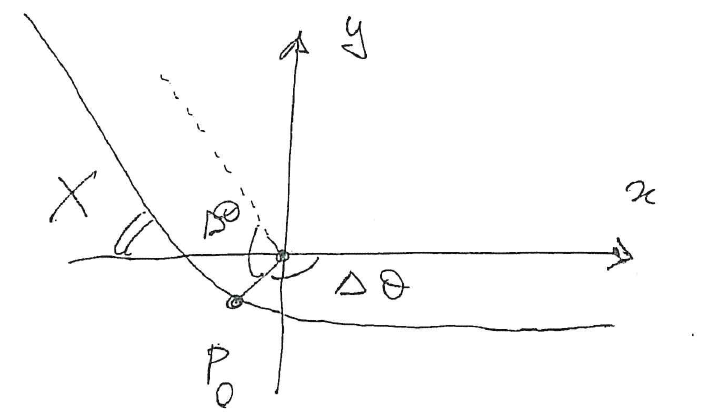
\includegraphics[width=0.6\linewidth]{sezione-urto}
	\caption{Schema della deflessione di una particella di un angolo \(\chi\).}
	\label{fig:sezione-urto}
\end{figure}
\FloatBarrier
Se abbiamo a che fare con un fascio di particelle uguali, che partono tutte a velocità uguali \((v_\infty)\) ma con p diversi, avremo $\chi$ di deflessione che variano con continuità in modo monotono dunque \(p(\chi)\) è invertibile in \(\chi(p)\). Abbiamo simmetria di rotazione, essendo il fascio cilindrico e centrato nell'asse del nucleo, quando il fascio viene deflesso forma una calotta sferica. Consideriamo la porzione di calotta sferica compresa fra gli angoli di deflessione \(\chi\) e $\chi+d\chi$, in questa regione passeranno, nell'unita di tempo, un numero dN di particelle. La grandezza dN non è indipendente dalle condizioni sperimentali in quanto più è denso il fascio più particelle troveremo, per trovare una grandezza che definisca il fenomeno in sè definiamo la sezione d'urto infinitesima
\[d\sigma = \frac{dN}{n}\]
dove n è la densità del fascio. Il nome sezione d'urto è dovuto solamente al fatto che ha le dimensioni di un'area ma in realtà è interpretabile come il valore atteso di particelle rilevate nell'unità di tempo nella regione considerata. Nella regione saranno diffuse solamente le particelle di parametro d'urto compreso fra \(p(\chi)\) e \(p(\chi+d\chi) = p(\chi)+dp(\chi)\). Il numero di particelle dN è calcolabile osservando che queste stesse particelle deflesse stavano nel fascio in una corona circolare di area \((2\pi pdp)\)
\[dN = n(2\pi pdp)\]
\[d\sigma = 2\pi pdp\]
possiamo infine trovare la relazione fra sezione d'urto e angolo di deflessione 
\[d\sigma(\chi) = 2\pi p(\chi)\frac{\partial p}{d\chi}d\chi\]
solitamente all'aumentare del parametro d'urto l'angolo di deflessione diminuisce, la derivata è solitamente negativa dunque si usa scrivere
\[d\sigma(\chi) = 2\pi p|\frac{\partial p}{\partial\chi}|d\chi\]
Possiamo infine riesprimere questa relazione usando gli angoli solidi:
\[d\omega = 2\pi\sin\chi d\chi\]
\[d\sigma = \frac{p(\chi)}{\sin\chi}|\frac{\partial p}{\partial \chi}|d\omega \]
Questa relazione può ad esempio essere usata per verificare se i risultati teorici sono corretti: teoricamente, in base al tipo di interazione che suppongo, otterrò un certo \(p(\chi)\) da cui prevederò una sezione d'urto \(\sigma (\chi)\), la sezione d'urto è misurabile a partire dalle rilevazioni delle particelle deflesse.\\
Storicamente un famoso esperimento che coinvolge la sezione d'urto è quello svolto da Rutherford per verificare la validità del modello atomico detto a panettone e che invece, confutandolo, portò a nuove teorie atomiche. Rutherford ipotizzava che la repulsione sarebbe avvenuta a causa del campo coulombiano dei nuclei dunque \(U=\frac{\alpha}{r}\), che è un potenziale kepleriano. L'equazione dell'angolo in funzione del raggio è
\[\Delta\theta=\int_{r_{min}}^{\infty}\frac{p_{\phi}dr}{r^2\sqrt{2m(E-U(r))-\frac{p_\phi^2}{r^2}}}\]
che, come ricavato precedentemente, porta all'equazione delle orbite 
\[r=\frac{p}{1+e\cos\theta}\]
per come è stata ricavata questa relazione sappiamo che al pericentro \(\theta = 0\) mentre all'infinito
\[\cos\theta = -\frac{1}{e}\]
osservando che \(\Delta\theta\) è l'angolo spazzato dal pericentro all'infinito, si ha che \(\cos\Delta\theta = -\frac{1}{e}\);
il segno è irrilevante in quanto nella formula della sezione d'urto compare con il valore assoluto. Sostituendo la definizione di e
\[\cos(\Delta\theta) = \frac{1}{e} = \frac{1}{\sqrt{1+\frac{2Ep_\theta^2}{mk^2}}}\]
\[\sin(\Delta\theta)  = \frac{\sqrt{\frac{2E}{mk^2}}p_\theta}{\sqrt{1+\frac{2Ep_\theta^2}{mk^2}}}\]
dove si è usato
\[\sin^2x+\cos^2x = \sin^2x+\frac{1}{1+x^2} = 1\]
Possiamo dunque scrivere la tangente e differenziare
\[\tan(\Delta\theta) = \sqrt{\frac{2E}{mk^2}}p_\theta = \sqrt{\frac{2E}{mk^2}}mv_\infty p\]
\[d\tan(\Delta\theta) = \frac{d\Delta\theta}{\cos^2\Delta\theta} = \sqrt{\frac{2E}{mk^2}}mv_\infty dp\]
\[|\frac{dp}{d\Delta\theta}| =\frac{1}{\sqrt{\frac{2Em}{k^2}}v_\infty}\frac{1}{\cos^2\Delta\theta}\]
sostituisco \(v_\infty\) usando l'energia ed esprimo la relazione in funzione di $\chi$
\[\frac{dp}{d\Delta\theta} = \frac{dp}{d\chi}\frac{d\chi}{\Delta\theta} = 2\frac{dp}{d\chi}\]
\[|\frac{dp}{d\chi}| =\frac{1}{2}\frac{1}{\frac{2E}{k}}\frac{1}{\sin^2\frac{\chi}{2}}\]
integrando si ottiene 
\[p(\chi) = -\frac{1}{\frac{2E}{k}}\cot\frac{\chi}{2}\]
Sostituendo nella formula generale della sezione d'urto si ottiene la formula di Rutherford
\[d\sigma = -\frac{1}{\left(\frac{2E}{k}\right)^2}\cot\frac{\chi}{2}\frac{1}{2\sin\chi}\frac{1}{\sin^2\frac{\chi}{2}}d\omega \]


\newpage
\section{Piccole oscillazioni}
Consideriamo una lagrangiana indipendente dal tempo con potenziali dipendenti unicamente dalla posizione, un punto x è stabile per il potenziale se è un suo punto critico
\[x\ d'\ equilibrio \leftrightarrow \frac{\partial U}{\partial x^j} = 0\]
un punto è detto di equilibrio stabile se è un minimo ed instabile se è un massimo. Se dunque il punto è di equilibrio stabile l'hessiana del potenziale sarà definita positiva. Questi concetti possono essere equivalentemente espressi in termini di stabilità secondo Ljapunov
\begin{definizione}[Stabilità secondo Ljapunov]
	Un punto di equilibrio è detto stabile (secondo Ljapunov) se ogni orbita del sistema che parte sufficientemente vicina al punto di equilibrio rimane nelle vicinanze del punto di equilibrio.
\end{definizione}
Graficamente, un punto di equilibrio stabile sta in una buca di potenziale, se viene perturbato la sua posizione cambia e il potenziale sicuramente aumenta (def. di minimo) ma se l'energia si conserva e il potenziale aumenta, allora l'energia cinetica deve diminuire, e dunque la velocità deve diminuire, fino a far fermare la particella. La particella è intrappolata in un intorno del punto di equilibrio stabile e questo intorno dipende dall'energia del sistema.\\
Sia \(\hat{q}\) il punto d'equilibrio stabile e \(\eta\in [-\varepsilon,\ \varepsilon]\) con $\varepsilon$ piccolo a piacere. Un generico punto contenuto nell'intorno del punto di equilibrio stabile sarà del tipo \(q = \hat{q}+\eta\).
Osservando che una lagrangiana quadratica in \(q\) e \(\dot{q}\), una volta applicato l'operatore di Lagrange, porta ad equazioni del moto lineari, che in generale sono di più facile risoluzione, vogliamo sviluppare in serie di Taylor la Lagrangiana nell'intorno del punto d'equilibrio stabile in modo da avere solo termini quadratici.\\  
Sviluppiamo dunque al secondo ordine il potenziale nell'intorno del punto d'equilibrio stabile
\[U(q^i) = U(\hat{q}^i+\eta^i) = U(\hat{q}^i) + \frac{\partial U}{\partial q^i}|_{\hat{q}}\eta^i + \frac{1}{2} \frac{\partial^2 U}{\partial q^iq^j}|_{\hat{q}}\eta^i\eta^j+o(|\eta|^2)\]
il primo termine del secondo membro è una costante e la lagrangiana è definita a meno di una costante dunque si può eliminare, il secondo termine è nullo per definizione di punto di equilibrio stabile, dunque
\[U(q^i) = \frac{1}{2} \frac{\partial^2 U}{\partial q^iq^j}|_{\hat{q}}\eta^i\eta^j+o(|\eta|^2) = \frac{1}{2}\hat{h}_{ij}\]
dove \(\hat{H}\) è l'hessiana del potenziale calcolata nel punto d'equilibrio stabile, che è un tensore di rango (2, 0) definito positivo.\\
Osservando che l'energia cinetica è definita mediante una forma quadratica, e che quindi ogni sviluppo superiore all'ordine zero porterebbe a termini di grado superiore a 2, sviluppiamo l'energia cinetica all'oridine 0, cioè la calcoliamo in $q = e\hat{q}$
\[T \simeq \frac{1}{2}\hat{g}_{ij}\dot{\eta}^i\dot{\eta}^j\]
dove \(\hat{g}_{ij}\) (o in forma matriciale \(\hat{G}\)) è il tensore metrico calcolato nel punto d'equilibrio stabile. Ne segue che la lagrangiana delle piccole oscillazioni è 
\[\mathcal{L}_{p.o.} = \frac{1}{2}\left(\dot{\eta}^i\hat{g}_{ij}\dot{\eta}^j-\eta^i\hat{h}_{ij}\eta^j\right)\]
Applicando l'operatore lagrangiano si ottengono le equazioni del moto per piccole oscillazioni
\[\hat{g}_{ij}\ddot{\eta}^j+\hat{h}_{ij}\eta^j = 0\]
che è un sistema di equazioni differenziali omogenee del secondo ordine.
Imponiamo che la soluzione sia del tipo
\[\eta^j = \eta_\lambda^j e^{\lambda t}\]
sostituendo nella relazione precedente si ottiene
\[\lambda^2\hat{g}_{ij}+\hat{h}_{ij} = 0\]
ma essendo sia metrica che hessiana definite positive (rispettivamente perché l'energia cinetica è positiva e perché siamo nell'intorno di un minimo) per soddisfare questa relazione deve essere \(\lambda^2<0\) da cui $\lambda = \pm i\omega$ dunque la soluzione relativa all'autovalore $\lambda$ è del tipo
\[\eta^j = \eta_\omega^j\left(A_{\omega}e^{i\omega t} + B_{\omega}e^{-i\omega t}\right)\]
di cui la soluzione fisica è costituita dalla parte reale. Osservando che la parte reale di questa espressione è la medesima della parte reale di
\[\eta^j = C_{\omega}\eta_{\omega}^je^{-i\omega t}\]
poiché entrambe possono essere espresse nella forma
\[Re(\eta^j) = \sum_\omega \eta_\omega^jf_\omega\cos(\omega t + \phi_\omega)\]
imponiamo questa soluzione per semplicità. C è un fattore di scala uguale per tutti gli indici, $\omega$ una costante e le \(\eta_{\omega}^j\) sono componenti controvarianti di un vettore da determinare che esprime l'ampiezza delle oscillazioni di ogni componente. Sostituendo
\[\hat{g}_{ij}\frac{d^2}{dt^2}{\eta}^j+\hat{h}_{ij}\eta^j= \left(-\hat{g}_{ij}\omega^2C_{\omega}\eta_{\omega}^j+\hat{h}_{ij}C_{\omega}\eta_{\omega}^j\right)e^{-i\omega t} = 0\]
L'esponenziale e \(C_{\omega}\) non si possono annullare dunque li semplifichiamo, ottenendo un sistema lineare omogeneo a coefficienti costanti, di incognita \(\eta_{\omega}^j\)
\[\hat{h}_{ij}\eta_{\omega}^j-\hat{g}_{ij}\omega^2\eta_{\omega}^j = 0\]
la matrice associata al sistema lineare è
\[\left(\hat{h}_{ij}-\hat{g}_{ij}\omega^2\right)\]
dalla teoria sui sistemi lineari sappiamo che se il determinante di questa matrice fosse nullo, tutte le equazioni sarebbero linearmente indipendenti dunque l'unica soluzione sarebbe quella banale \(\eta_{\omega}^j = 0\), che equivarrebbe ad un sistema fermo. Per evitare la soluzione banale imponiamo il determinante nullo
\[det\left(\hat{h}_{ij}-\hat{g}_{ij}\omega^2\right) = 0\]
da cui troviamo un vincolo che ci permette di determinare la costante $\omega$, per un sistema lineare n-dimensionale otterremo n $\omega$ diverse. Le soluzioni in generale potrebbero ripetersi ma consideriamo solo il caso di $\omega$ tutti distinti. Le $\omega$ ottenute sono interpretabili come le frequenze per le quali la soluzione imposta è corretta.\\
Tornando alla risoluzione del sistema lineare, vogliamo determinare le \(\eta_{\omega}^j\), osserviamo che questo problema si presenta come la generalizzazione del problema della ricerca degli autovalori di una matrice: vogliamo trovare gli \(\eta_{\omega}^j\) tali che
\[\hat{h}_{ij}\eta_{\omega}^j = \lambda \hat{g}_{ij}\eta_{\omega}^j\]
con \(\lambda = \omega^2\)che differisce dal problema agli autovalori per la presenza della metrica.\\
Come dimostrato in appendice \ref{ap:autoval}, essendo $\hat{H}$ e \(\hat{G}\) simmetriche, un problema siffatto ammette autovalori tutti reali e positivi, gli autovettori associati agli autovalori $\lambda$ sono ortogonali rispetto al prodotto scalare con matrice associata $\hat{g}_{ij}$ e la matrice con gli autovettori sulle colonne è una matrice cambio di base che diagonalizza sia $\hat{H}$ che $\hat{G}$, tale che $\hat{G}$ nella nuova base è l'identità ed $\hat{H}$ nella nuova base presenta gli autovalori sulla diagonale. Dunque gli \(\eta_{\omega}^j\) sono gli autovalori di \(\hat{H}\). La lagrangiana, a seguito del cambio di base, diventa
\[\mathcal{L}_{P.O.} = \sum_\omega\frac{1}{2} (\eta^j_\omega)^2-\frac{\omega}{2}(q^j)^2\]
Essendo questi autovettori ortonormali, sono fra loro indipendenti, cioè costituiscono una base di soluzioni. La soluzione generale può essere scritta come la combinazione lineare della base di soluzioni. Visto che ogni elemento della base di soluzioni rappresenta un moto oscillatorio ad una specifica frequenza d'oscillazione \(\omega\), dal punto di vista fisico la soluzione generale delle equazioni del moto sarà una sovrapposizione delle oscillazioni corrispondenti a tutte le frequenze possibili. In altre parole, se un sistema viene perturbato a partire da una posizione di equilibrio stabile compirà piccole oscillazioni che sono la sovrapposizione di oscillazioni di frequenze $\omega_1, ..., \omega_n$. Le singole soluzioni a frequenza fissata sono dette frequenze di risonanza del sistema. Possiamo scrivere la soluzione generale in forma vettoriale come
\[\eta (t) = \sum_\omega C_{\omega} \eta_{\omega}e^{-i\omega t} \]
\[\dot{\eta}(t) = -i\omega\sum_\omega C_{\omega} \eta_{\omega}e^{-i\omega t}\]
di cui dovremo prendere la parte reale della prima e la parte immaginaria della seconda. Per determinare completamente la soluzione, non ci resta che determinare le \(C_{\omega}\) imponendo 2n condizioni iniziali. Se le frequenze sono incommensurabili, cioè se ad esempio
\(\omega_i/\omega_j = \frac{\mathbb{R}}{\mathbb{Q}}\), allora le orbite non saranno chiuse ma sicuramente limitate. Queste orbite si chiamano quasi-periodiche e riempiono in maniera densa un intorno dell'equilibrio stabile. Le \(\omega\) sono dette frequenze delle piccole oscillazioni, gli autovettori ad esse associati sono detti modi normali d'oscillazione. 
\subsection{Piccole oscillazioni con potenziali generalizzati}
Nella precedente trattazione non abbiamo tenuto conto dei potenziali generalizzati, questo perché è facile mostrare che questi non influiscono nel moto delle piccole oscillazioni. Trattiamo ora il caso generale
\[\mathcal{L} = \frac{1}{2}\dot{q}^ig_{ij}\dot{q}^j-U(q)+kA(q)_i\dot{q}^i\]
Sviluppiamo i termini in modo da ottenere una lagrangiana quadratica: svilupperemo il potenziale generalizzato al primo ordine
\[\mathcal{L}_{P.O.} = \frac{1}{2}\dot{\eta}^ig^0_{ij}\dot{\eta}^j+k\frac{\partial A^0_i}{\partial q^j}\dot{\eta}^i\eta^j-\frac{1}{2}\eta^ih^0_{ij}\eta^j\]
applicando l'operatore di Lagrange, dal termine di potenziale generalizzato risulta un tensore antisimmetrico
\[\left(\frac{d}{dt}\frac{\partial}{\partial\ \dot{\eta}^j}-\frac{\partial}{\partial \eta^j}\right)\mathcal{L}_{P.O.} = 0 \]
\[\ddot{\eta}^i g^0_{ij}+k\left(\frac{\partial A^0_i}{\partial q^j}\delta^i_j\dot{\eta}^j-\frac{\partial A^0_i}{\partial q^j}\dot{\eta}^i\right)+\eta^ih^0_{ij}=0\]
\[\ddot{\eta}^i g^0_{ij}+ka^0_{ij}\dot{\eta}^i+\eta^ih^0_{ij}=0\]
dove abbiamo ridefinito la matrice risultante dal potenziale generalizzato \(a^0_{ij}\). Imponendo una soluzione del tipo\(\eta(t) = \eta_\lambda e^{\lambda t}\) otteniamo il sistema lineare
\[(\lambda^2 g^0_{ij}+ka^0_{ij}\lambda+h^0_{ij})\eta_\lambda^i=0\]
se moltiplichiamo per \(\eta_\lambda^j\) otteniamo delle forme quadratiche, in particolare quella relativa al potenziale generalizzato deve essere nulla perché prodotto di un tensore simmetrico per uno antisimmetrico
\[a^o_{ij}(\eta^i\eta^j) = 0\]
dunque ci riconduciamo al caso precedente in cui osserviamo che un \(\lambda^2\) che soddisfi questa relazione deve essere necessariamente negativo, da cui la soluzione complessa di cui sopra.
\begin{esercizio}[Pendolo doppio]
Consideriamo due ate rigide di massa trascurabile alle cui estremità sono attaccate due masse m puntiformi, le due aste formano un doppio pendolo come in figura
\begin{figure}[h!]
	\centering
	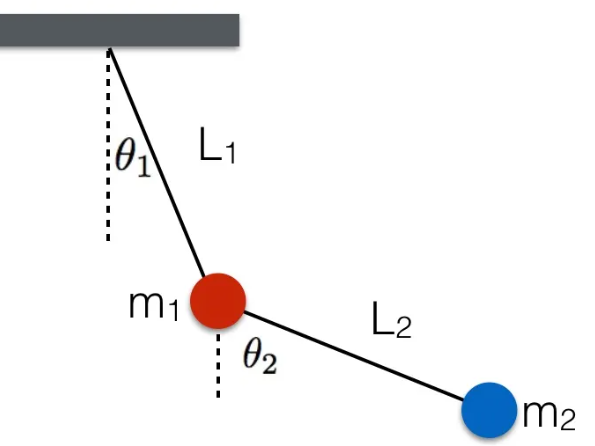
\includegraphics[width=0.6\linewidth]{doppio-pendolo}
	\caption{Schema del doppio pendolo, nel nostro caso \(m_1 = m_2\), \(L_1 = L_2\), \(\theta_1 = \theta\), \(\theta_2 = \phi\).}
	\label{fig:doppio-pendolo}
\end{figure}
\FloatBarrier	
Le coordinate e le velocità delle due masse sono
\begin{align*}
	\begin{cases}
		\mathbf{x}_1 = (L\sin\theta, -L\cos\theta)\\
		\mathbf{x}_2 = (l\sin\theta+L\sin\phi, -l\cos\theta-L\cos\phi)
	\end{cases}
	\begin{cases}
		\dot{\mathbf{x}}_1 = L\dot{\theta}(\cos\theta, \sin\theta)\\
		\dot{\mathbf{x}}_2 = L(\cos\theta\dot{\theta}+\cos\phi\dot{\phi}, \sin\theta\dot{\theta}+\sin\phi\dot{\phi})
	\end{cases}
\end{align*}
Dunque l'energia cinetica ed il potenziale risultano
\[T = \frac{m}{2}L^2\dot{\theta}^2+\frac{m}{2}L^2(\dot{\theta}^2+\dot{\phi}^2+2\dot{\theta}\dot{\phi}\cos(\theta-\phi)) = \frac{m}{2}L^2(2\dot{\theta}^2+\dot{\phi}^2+2\dot{\theta}\dot{\phi}\cos(\theta-\phi))\]	
\[V = -mgL(2\cos\theta +\cos\phi)\]
Abbiamo dunque una lagrangiana in due incognite con solamente l'energia come integrale primo: è un sistema non integrabile. Studiamo le piccole oscillazioni nell'intorno di un punto d'equilibrio stabile. Senza fare conti, risulta ovvio che il minimo del potenziale si ha quando \(\theta =\phi = 0\). L'hessiana e la metrica calcolate in \((0, 0)\) sono
\begin{align*}
	\hat{H} =
	\begin{pmatrix}
		2&0\\
		0&1
	\end{pmatrix}
mgL\\
\hat{G} =
\begin{pmatrix}
	2&1\\
	1&1
\end{pmatrix}
mL^2
\end{align*}
dunque l'equazione delle piccole oscillazioni (per trovare le frequenze delle piccole oscillazioni)	è
\[det(\omega^2\hat{G}-\hat{H}) = 0\]
\[2(\omega^2-\frac{g}{L})^2-\omega^4 = 0\]
\[\omega^2 = 2\omega_0^2\pm\sqrt{2}\omega_0^2\]
con \(\omega_0 = \sqrt{\frac{g}{l}}\)
Infine, otteniamo due frequenze delle piccole oscillazioni
\[\omega_+ = \sqrt{2+\sqrt{2}}\omega_0\]
\[\omega_- = \sqrt{2-\sqrt{2}}\omega_0\]
Dove la prima è maggiore della frequenza che avrebbe avuto il pendolo semplice mentre la seconda minore. Ricaviamo infine gli autovettori (modi normali d'oscillazione), cioè i vettori per cui vale
\[(\omega^2\hat{G}-\hat{H})q = 0\]
\begin{align*}
	\begin{pmatrix}
		-2mL^2\omega^2+2mgL&-m\omega^2L^2\\
		-m\omega^2L^2&-m\omega^2L^2+mgL
	\end{pmatrix}
\begin{pmatrix}
	\theta_\pm\\
	\phi\pm
\end{pmatrix}=0
\end{align*}
\begin{align*}
\begin{pmatrix}
2\pm2\sqrt{2}&2\pm\sqrt{2}\\
2\pm2\sqrt{2}&1\pm\sqrt{2}
\end{pmatrix}
\begin{pmatrix}
	\theta_\pm\\
	\phi\pm
\end{pmatrix}=0
\end{align*}
Le due righe della matrice sono linearmente dipendenti: ne prendo una, che mi esprime la relazione fra $\phi$ e \(\theta\) 
\begin{align*}
	\phi_\pm = -\theta_\pm\frac{2\pm2\sqrt{2}}{2-\sqrt{2}}
\end{align*}
Nel caso \(\omega_+\) il segno di \(\phi\) e \(\theta\) è diverso, oscillano in modo discorde, mentre nel caso \(\omega_-\) hanno stesso segno ed oscillano in modo concorde. 
	
	
	
	
	
	
	
	
	
	
	
	
	
	
	
\end{esercizio}
\newpage
\section{Dinamica e geometria}
Possiamo vedere un problema fisico in due modi equivalenti ma molto diversi:
\begin{itemize}
\item Dinamica: \\
un corpo, che in generale si muove in 3 dimensioni, è costretto a muoversi seguendo certe curve o superfici a causa di forze, dovute all'interazione fra particelle. In questa interpretazione, mediante il secondo principio della dinamica, risolvendo le equazioni differenziali, si ottengono le traiettorie parametrizzate dal tempo. In questo caso la metrica è sempre quella euclidea e per introdurre l'informazione sulle traiettorie si considerano forze esterne.
\item Geometrica: \\
un corpo è vincolato a muoversi su curve o superfici e non vive, in generale, in uno spazio tridimensionale. Al posto di inserire le forze e di usare la metrica euclidea si usa la metrica dello spazio in cui è vincolato a muoversi e quelle che nell'interpretazione dinamica erano forze esterne ora saltano fuori dall'energia cinetica, che è l'unica componente della lagrangiana, e che ha come matrice associata in generale qualcosa di più complesso dell'identità, e che quindi farà spuntare fuori nuovi termini. In questa interpretazione si perde l'informazione sul tempo, le traiettorie sono semplicemente date dalle superfici sullo spazio delle configurazioni e il parametro sarà generico, non più il tempo, parametro speciale.
\end{itemize}
Per passare dalla formulazione dinamica a quella geometrica basta considerare la forza come un vincolo sullo spazio delle configurazioni, e cercare coordinate adattate al vincolo in modo da ridurre i gradi di libertà al minimo, in questo modo la metrica cambia e l'effetto della forza è inglobata in essa. Questo è possibile solamente se la forza agisce unicamente sullo spazio delle configurazioni e non impone vincoli sulle velocità, in questo caso si tratterà di un vincolo anolonomo per il quale non è possibile trovare coordinate generalizzate adatte.
\begin{esempio}[Relatività generale] 
 	Questa idea è stata sfruttata da Einstein nella formulazione della relatività generale: la forza di gravità non è più vista come tale ma come deformazione dello spaziotempo, ovvero lo spazio in cui vivono i corpi, i moti dei pianeti, ad esempio le orbite ellittiche, in quest'ottica, non sono dovute alla forza esercitata da corpi massicci ma dalla deformazione dello spazio che questi provocano.
\end{esempio}
\begin{osservazione}[Forze vincolari]
	Immergendo un sistema vincolato (e dunque un sistema fisico interpretato geometricamente) in uno spazio euclideo di dimensione superiore, quello che sembrava un vincolo nell'interpretazione geometrica, risulterà pari alla forza vincolare nell'interpretazione dinamica.
\end{osservazione} 
\subsection{Il problema delle geodetiche}
Il principio di minima azione ci avvicina ad un'interpretazione geometrica della fisica: in particolare, considerando una particella libera, trovare il percorso che minimizza la sua azione, ovvero l'integrale di percorso della lagrangiana, che in questo caso è semplicemente uguale all'energia cinetica, ovvero la forma quadratica con associata la metrica, è un problema puramente geometrico, detto problema delle geodetiche.
\begin{osservazione}[Caratterizzazione delle geodetiche]
	Le geodetiche possono essere definite come le curve su una superficie la cui normale è diretta come la normale alla superficie.
\end{osservazione}
Possiamo sviluppare questo problema in modo equivalente usando l'interpretazione dinamica o geometrica. Questo esempio mette in luce come interpretazione dinamica e geometrica siano legate dal principio di minima azione.
\subsubsection{Interpretazione dinamica}
Da un punto di vista dinamico, la determinazione delle geodetiche equivale a determinare l'equazione della traiettoria che minimizza il funzionale d'azione della particella libera.\\
Abbiamo già risolto il problema delle geodetiche in coordinate cartesiane senza saperlo quando abbiamo ricavato la lagrangiana dal principio di minima azione: applicando l'operatore di Lagrange alla particella libera, con metrica euclidea, si ottiene (poniamo m = 1 per semplicità)
\[\delta\int_{t_A}^{t_b}\frac{1}{2} v^i\delta_{ij}v^jdt = 0\]
\[\leftrightarrow \frac{d}{dt}\left(\frac{\partial}{\partial v}\frac{1}{2} v^2\right) = 0\]
\[v= \frac{dx}{dt} = c_1\]
\[x(t) = c_1 t + c_2 \]
da cui deriva il fatto che il percorso che minimizza la lagrangiana in questo caso è quello percorso a velocità costante, e che l'equazione della geodetica è una retta (\(c_1\) sarà la velocità iniziale e \(c_2\) la posizione iniziale).\\
Più in generale, posso considerare una metrica qualsiasi
\[\mathcal{L} = T =\frac{1}{2}\dot{q}^ig_{ij}\dot{q}^j\]
\[\delta S = \delta \int_{t_a}^{t_b}\frac{1}{2}\dot{q}^ig_{ij}\dot{q}^j dt =0 \]
questa espressione definisce in generale le geodetiche usando un approccio dinamico. Si osservi che il parametro delle curve è il tempo. Applichiamo l'operatore lagrangiano
\[\left(\frac{d}{dt}\frac{\partial }{\partial \dot{q}^j}-\frac{\partial }{\partial q^j}\right)\left(\frac{1}{2}\dot{q}^ig_{ij}\dot{q}^j\right) = 0\]
\[\frac{d}{dt}\left(\dot{q}^ig_{ij}\right)-\frac{1}{2}\dot{q}^i\frac{\partial g_{ij}}{\partial q^j}\dot{q}^j = 0\]
sviluppo la derivata di prodotto nel primo termine, osservando che la metrica dipende solo da \(q\)
\[\ddot{q}^ig_{ij}+ \dot{q}^i\left(\frac{d}{dt}g_{ij}(q^j(t))\right)-\frac{1}{2}\dot{q^i}\frac{\partial g_{ij}}{\partial q^j}\dot{q}^j = 0\]
sviluppo la derivata della metrica con la regola della catena
\[\ddot{q}^ig_{ij}+ \dot{q}^i\frac{\partial g_{ij}}{\partial q^j}\dot{q}^j-\frac{1}{2}\dot{q^i}\frac{\partial g_{ij}}{\partial q^j}\dot{q}^j = 0\]
\[\ddot{q}^ig_{ij}+\frac{1}{2}\dot{q^i}\frac{\partial g_{ij}}{\partial q^j}\dot{q}^j= 0\]
ma questa espressione equivale a
\[\frac{d}{dt}\left(\dot{q}^ig_{ij}\dot{q}^j\right) = 0\]
infatti, sviluppando due volte la derivata di prodotto si ottiene
\[\frac{d}{dt}\left(\dot{q}^i\cdot(g_{ij}\dot{q}^j)\right) = \ddot{q}^ig_{ij}\dot{q}^j + \dot{q^i}\frac{d}{dt}\left( g_{ij}\cdot \dot{q}^j \right) = \]
\[\ddot{q}^ig_{ij}\dot{q}^j + \dot{q^i}\left(\dot{q}^i\frac{\partial g_{ij}}{\partial q^i}\dot{q}^j+ g_{ij}\ddot{q}^j \right)= \]
ma essendo i e j dummy indexes, li posso invertire, sommare primo e terzo termine e dividere tutto per due
\[=\frac{1}{2}\dot{q}^i\dot{q}^i\frac{\partial g_{ij}}{\partial q^i}\dot{q}^j+ \dot{q}^i\dot{q}^ig_{ij}\ddot{q}^j =
\dot{q}^i\left(\frac{1}{2}\dot{q}^i\frac{\partial g_{ij}}{\partial q^i}\dot{q}^j+ \dot{q}^ig_{ij}\ddot{q}^j\right) = 0\]
semplificando \(\dot{q}^i\) riotteniamo l'espressione precedente.
Riassumendo:
\[\frac{d}{dt}\left(\dot{q}^ig_{ij}\dot{q}^j\right) = 0\]
essendo per definizione il modulo della velocità 
\[|v| \equiv \sqrt{\dot{q}^ig_{ij}\dot{q}^j}\]
la condizione che una traiettoria sia una geodetica equivale a dire che il modulo della velocità sia costante
\[|v| = \frac{ds}{dt} = cost.\]
si osservi il fatto fondamentale che la velocità è definita come \(\frac{ds}{dt}\) dove al denominatore è presente lo speciale parametro tempo, che lo rende diverso da tutti gli altri proprio perché compare in questa definizione. Questo esaurisce la trattazione delle geodetiche con interpretazione dinamica.
\subsubsection{Interpretazione geometrica}
Possiamo sviluppare il problema delle geodetiche da un punto di vista prettamente geometrico senza alcuna analogia fisica per poi mostrare l'equivalenza dei due problemi. Cominciamo con il definire la lunghezza infinitesima di una curva su una varietà riemanniana X come la forma quadratica, con matrice associata la metrica, definita sugli spostamenti infinitesimi, sotto radice.
\[ds = \sqrt{d{q}^ig_{ij}d{q}^j}\] 
data una curva $q(\alpha): [\alpha_a, \alpha_b]\rightarrow X$ definita tra due punti fissati \(q(\alpha_a) = q_a\), \(q(\alpha_b) = q_b\), definiamo la lunghezza d'arco come
\[S =\int_{q_a}^{q_b}ds = \int_{q_a}^{q_b}\sqrt{d\dot{q}^ig_{ij}d\dot{q}^j}= \int_{q_a}^{q_b}\sqrt{d{q}^ig_{ij}d{q}^j} \frac{d\alpha}{d\alpha} =\] \[\int_{q_a}^{q_b}\sqrt{\frac{d{q}^i}{d\alpha}g_{ij}\frac{d{q}^j}{d\alpha}}d\alpha = \int_{q_a}^{q_b}\sqrt{q'^ig_{ij}q'^j}d\alpha \]  
dove l'apice indica la derivata rispetto al parametro $\alpha$ (mentre la derivata rispetto al tempo, parametro speciale, è indicata con il punto sopra la variabile).
\begin{definizione}[geodetica]
	Dato uno spazio metrico X, una curva $\gamma: I\rightarrow X$, \(I=[t_a,\ t_b]\in \mathbb{R}\), tale da avere lunghezza minima, è detta geodetica. La forma della geodetica dipende unicamente dalla metrica dello spazio considerato.
\end{definizione}
dunque, la curva \(q(\alpha)\) è una geodetica, come da definizione, se la lunghezza d'arco fra i due punti fissati è minima. Questa condizione, esprimibile mediante principio variazionale, non dipende dal parametro ed è puramente geometrica:
\[\delta S = \delta\int_{q_a}^{q_b}\sqrt{q'^ig_{ij}q'^j}d\alpha = 0\]
come dimostrato in precedenza, \(q(\alpha)\) soddisfa questo problema variazionale se e solo se soddisfa
\[\left(\frac{d}{d\alpha}\frac{\partial }{\partial q'^j}-\frac{\partial }{\partial q^j}\right)\left(\sqrt{q'^ig_{ij}q'^j}\right) = 0\]
\[\frac{d}{d\alpha}\left(\frac{q'^ig_{ij}}{\sqrt{q'^ig_{ij}q'^j}}\right)-\frac{1}{2}\frac{q'^i\frac{\partial g_{ij}}{\partial q^j}q'^j}{\sqrt{q'^ig_{ij}q'^j}} = 0\]
questo esaurisce il problema delle geodetiche in interpretazione geometrica.\\
\subsubsection{equivalenza degli aprocci}
I due approcci portano apparentemente a risultati diversi. Osserviamo tuttavia che la differenza fondamentale è che nell'approccio dinamico abbiamo scelto un parametro speciale mentre in quello geometrico abbiamo un parametro generale. Se in quest'ultimo approccio usiamo il tempo otteniamo, ricordando la definizione di velocità (sappiamo che questa è costante lungo le geodetiche da quanto ottenuto con approccio dinamico)
\[\frac{d}{dt}\left(\frac{\dot{q}^ig_{ij}}{|v|}\right)-\frac{1}{2}\frac{\dot{q}^i\frac{\partial g_{ij}}{\partial q^j}\dot{q}^j}{|v|} = 0\]
semplifico \(|v|\), che è una costante positiva
\[\frac{d}{dt}\left({\dot{q}^ig_{ij}}\right)-\frac{1}{2}{\dot{q}^i\frac{\partial g_{ij}}{\partial q^j}\dot{q}^j} = 0\]
che è proprio quanto ottenuto nell'interpretazione dinamica, sviluppando riotterremo lo stesso risultato finale.\\
In conclusione, deduciamo che l'interpretazione geometrica è una generalizzazione di quella dinamica, che prende come parametro un generico $\alpha$ invece che il tempo; è sempre possibile passare dall'interpretazioen geometrica a quella dinamica sostituendo il parametro. In generale il funzionale mediante il quale si definiscono le geodetiche geometricamente è diverso da quello dinamico, cioè il funzionale d'azione, finché non scelgo il parametro tempo. L'approccio geometrico è talvolta utile perché permette di prendere come parametro una delle variabili del problema, ovvero il tempo, riducendo di 1 i d.o.f., a prezzo di perdere l'informazione sul tempo.  
\subsection{La catenaria}
Un esempio in cui l'analogia fra interpretazione dinamica e geometrica mostra la sua potenza è quello del problema catenaria. Il problema, puramente geometrico, è il seguente: data una corda massiccia, soggetta a forza di gravità, di lunghezza L, fissata a due punti A e B di altezza h, tali che \(|AB|<L\), vogliamo trovare la funzione che segue la corda all'equilibrio. Vogliamo applicare il principio di minima azione, dunque calcoliamo la lagrangiana: l'energia cinetia è nulla perché la corda è in quiete e all'equilibrio, la lagrangiana coincide con l'energia potenziale della corda. Il problema però non è risolubile applicando direttamente il formalismo lagrangiano in quanto la corda è formata da infiniti punti e dunque ha infiniti gradi di libertà (uscirebbero infinite equazioni del moto). Imponiamo che il potenziale della corda, sia minimo: se riusciamo a trovare un funzionale che esprime l'energia potenziale della corda e costruiamo un principio variazionale con questo possiamo aggirare il problema. \\
Parametrizziamo la corda con \((x, y(x)) = \gamma(x)\), il potenziale gravitazionale è \(U(x) = mgy\) ma la massa da considerare è quella della porzione infinitesima di corda, usiamo la densità lineare di massa
\[\rho = \frac{M}{L}\]
\[dm = \rho ds\]
dove ds è l'elemento infinitesimo di lunghezza, definito, come visto sopra, come
\[ds = \sqrt{dq^ig_{ij}dq^j}\]
visto che stiamo usando la metrica euclidea e siamo in coordinate cartesiane abbiamo
\[ds = \sqrt{dx^2+dy^2} = \sqrt{1+\left(\frac{dy}{dx}\right)^2}dx =\sqrt{1+y'^2}dx \]
l'energia potenziale dell'intera corda, ponendo l'origine degli assi nel mezzo di AB, definendo \(|AB|\equiv 2a\) è dunque
\[U[\gamma] = \int^{a}_{-a}\rho ds g y = \int^{a}_{-a}\rho g y\sqrt{1+y'^2}dx\]
che è un funzionale. Non è però sufficiente minimizzare questo funzionale in quanto ho una condizione sulla corda: questa ha una lunghezza L fissata, ciò si esprime come segue
\[L = \int^{a}_{-a}ds = \int^{a}_{-a}\sqrt{1+y'^2}dx>2a\]
Il problema di minimizzare il funzionale avendo una condizione è detto problema di ricerca dei minimi vincolati e si risolve usando i moltiplicatori di Lagrange: il funzionale da minimizzare sarà
\[\mathcal{F}[\gamma] = U[\gamma]-\lambda\int^{a}_{-a}\sqrt{1+y'^2}dx = \int^{a}_{-a}(\rho g y - \lambda)\sqrt{1+y'^2}dx \]
questo funzionale è l'analogo dell'azione, la nostra "lagrangiana" è
\[(\rho g y - \lambda)\sqrt{1+y'^2}\]
parametrizzata dal parametro x. Risolvere un problema del genere sappiamo essere equivalente a risolvere un'equazione di Eulero-Lagrange del tipo
\[\left(\frac{d}{dx}\frac{\partial }{\partial y'}-\frac{\partial}{\partial y}\right) \left((\rho g y - \lambda)\sqrt{1+y'^2}\right) = 0\]
non dipendendo la "lagrangiana" esplicitamente da x, che possiamo interpretare come il tempo, abbiamo sempre un'integrale del moto analogo all'energia
\[E = y'\frac{\partial}{\partial y'}(\rho g y - \lambda)\sqrt{1+y'^2}-(\rho g y - \lambda)\sqrt{1+y'^2} = \]
\[(\rho g y - \lambda)\frac{y'^2}{\sqrt{1+y'^2}}-(\rho g y - \lambda)\sqrt{1+y'^2} = \]
moltiplico e divido il secondo termine per \(\sqrt{1+y'^2}\) e semplifico
\[-\frac{(\rho g y - \lambda)}{\sqrt{1+y'^2}}\]
come sempre, possiamo vedere l'espressione dell'energia come un'equazione differenziale da manipolare e risolvere.Di seguito presentiamo i passaggi di manipolazione
\[E\sqrt{1+y'^2} = -(\rho g y - \lambda)\]
\[(1+y'^2) = \frac{(\rho g y - \lambda)^2}{E^2}\]
\[y'= \frac{dy}{dx} = \sqrt{\frac{(\rho g y - \lambda)^2}{E^2}-1}\]
\[dx = \frac{dy}{\sqrt{\frac{(\rho g y - \lambda)^2}{E^2}-1}}\]
sostituisco \(u = \frac{(\rho gy-\lambda)}{E}\); \(du = \frac{\rho g}{E}dy\)
\[dx  = \frac{E}{\rho g}\frac{du}{\sqrt{u^2-1}}\]
\[x(u) = \frac{E}{\rho g}arcosh(u) \]
\[x(y) = \frac{E}{\rho g}arcosh(\frac{(\rho gy-\lambda)}{E})\]
\[\frac{(\rho gy-\lambda)}{E} = \cosh(\frac{\rho g}{E}x)\]
\[y  = \frac{E}{\rho g}\cosh(\frac{\rho g}{E}x)+\frac{\lambda}{\rho g}\]
questa è l'equazione della catenaria, con i parametri E e \(\lambda\) da determinare. Per determinare E sostituisco $\lambda$ nel vincolo sulla lunghezza della corda, innanzitutto calcolo \(y'\) e poi $\sqrt{1+y'^2}$
\[y' = \frac{dy}{dx} = \sinh(\frac{\rho g}{E}x)\]
\[\sqrt{1+y'^2} = \sqrt{1+\sinh^2(\frac{\rho g}{E}x)} = \cosh(\frac{\rho g}{E}x) \]
\[L = \int_{a}^{-a}\cosh(\frac{\rho g}{E}x)dx = 2\int_{a}^{0}\cosh(\frac{\rho g}{E}x)dx = 2\frac{E}{\rho g}\sinh(\frac{\rho g}{E}a)\]
\[E = \frac{Lg\rho}{2}\frac{1}{\sinh(\frac{\rho g}{E}a)}\]
che fissa il valore di E. \\
$\lambda$ determina l'altezza a cui sono posti i punti A e B. Imponiamo che questa altezza sia uguale per entrambi, pari ad h, costante nota.
\[y(a) = y(-a) = \frac{Lg\rho\cosh(\frac{\rho g}{E}a)}{2\sinh(\frac{\rho g}{E}a)} = h\] 
 Senza perderci nelle costanti, osserviamo che la funzione che segue la corda è del tipo
\[y(x) = \overline{a}\left(1-\overline{b}\cosh(\overline{a}\overline{b}x)\right)\]
che è l'equazione di una catenaria.
\begin{osservazione}[Dinamica e geometria]
	Abbiamo risolto un problema puramente geometrico con un analogia dinamica: l'iter seguito è quello per determinare la traiettoria di un punto materiale di lagrangiana
	\[\mathcal{L} = (\rho g q(t) - \lambda)\sqrt{1+\dot{q}^2(t)}\]
	vincolato a passare per i punti A e B.
\end{osservazione}
\begin{osservazione}[Energia ed interpretazione geometrica]
	Si dimostra che scegliendo come parametro il tempo si conserva l'Energia a causa di una simmetria fisica del tempo. Questa legge di conservazione è dunque strettamente legata alle caratteristiche peculiari del tempo. Cosa succederebbe se applicassimo la definizione di energia ad un principio variazionale geometrico, cioè ad una "lagrangiana" che abbia come parametro un generico $\alpha$ e non il tempo? Consideriamo la "lagrangiana" del problema delle geodetiche con interpretazione geometrica
	\[\mathcal{L} = \sqrt{q'(\alpha)G(q(\alpha))q'(\alpha)}\]
	adattando la definizione di energia a questo caso otteniamo 
	\[E = q'\left(\frac{\partial }{\partial q'}\sqrt{q'Gq'}\right)-\sqrt{q'Gq'}=\]
	\[q'\frac{q'G}{\sqrt{q'Gq'}}-\sqrt{q'Gq'} = \sqrt{q'Gq'}-\sqrt{q'Gq'} = 0 \]
	osserviamo che l'energia resta un integrale del moto ma diventa banale, non è più utilizzabile, poiché l'energia è definita a meno di una costante. Con l'approccio geometrico dunque perdiamo tempo ed energia, che sono strettamente correlati. 
\end{osservazione}
\subsection{La metrica di Poincarè}
\begin{definizione}[Semispazio e metrica di Poincaré]
	Sia 
	\[H^n = \{(x^1, ..., x^n)\}\in\mathbb{R}^n: x^n>0 \]
	dove \(x^n\) è l'ultima componente dei vettori, un semispazio su cui è definita la metrica
	\[g_{ij} = \frac{\delta_{ij}}{(x^n)^2}\]
	detta metrica di Poincaré. E dunque la distanza
	\[ds^2 = \frac{dx^i\delta_{ij}dx^j}{(x^n)^2}\] 
	 Allora la coppia (\(H^n, ds^2\)) è detta semispazio metrico n-dimensionale di Poincaré.
\end{definizione}	
\begin{osservazione}
	La metrica di Poincaré in forma matriciale è\[G = \frac{I}{(x^n)^2}\], che è diagonale, ne segue che è un metrica euclidea riscalata di un fattore che dipende dal punto considerato. In particolare, se \(x^n \rightarrow \infty\), il tensore metrico tende ad annullarsi, dunque le distanza diminuiscono al'aumentare dell'ultima componente dei vettori fino ad annullarsi. Notiamo inoltre che il tensore metrico di Poincaré è definito positivo. 
\end{osservazione}
\begin{definizione}[Varietà riemanniana]
	Varietà differenziale M con associato un tensore metrico definito positivo. In questo modo è possibile indurre un prodotto scalare definito positivo sullo spazio tangente ad M (lo spazio in cui vivono le velocità), che permette di introdurre nozioni tipiche dello spazio euclideo, cioè angoli, distanze, geodetiche...
\end{definizione}
\begin{osservazione}
	In semispazio di Poincaré è una varietà riemanniana, possiamo dunque chiederci quali siano le geodetiche.
\end{osservazione}
Consideriamo un semipiano di Poincaré, ovvero un semispazio di Poincaré bidimensionale ( \(q = (x, y)\)): scriviamo la lagrangiana di una particella libera in questo spazio in forma vettoriale
\begin{align*}
	&\mathcal{L} = T = \frac{1}{2}\dot{q} G \dot{q} =
	 \frac{1}{2}
	 \begin{pmatrix}
	 	\dot{x}&\dot{y}
	 \end{pmatrix}
 \begin{pmatrix}
 	\frac{1}{y^2}&0\\
 	0&\frac{1}{y^2}
 \end{pmatrix}
\begin{pmatrix}
	\dot{x}\\
	\dot{y}
\end{pmatrix}= \frac{1}{2y^2}(\dot{x}^2+\dot{y}^2) = E
\end{align*}
osservo che x è una variabile ciclica: il momento associato è dunque un'integrale del moto
\[\frac{\partial \mathcal{L}}{\partial \dot{x}} = \frac{\dot{x}}{y^2} = p_x= cost.\]
\[E = \frac{\dot{x}^2}{2y^2}+\frac{\dot{y}^2}{2y^2} = \frac{p_x^2y^2}{2}+\frac{\dot{y}^2}{2y^2}\]
risolvo l'equazione differenziale 
\[dt = \frac{dy}{y\sqrt{2E}\sqrt{1-\frac{p_x^2}{2E}y^2}}\]
cambio variabile \(z = \frac{p_x}{\sqrt{2E}}y\); \(dz = \frac{p_x}{\sqrt{2E}}dy\)
\[dt = \frac{dz}{\sqrt{2E}\sqrt{1-z^2}z}\]
cambio variabile \(z = \sin(u)\); \(dz = \cos(u)du\)
\[dt = \frac{du}{\sqrt{2E}\sin (u)}\]
\[\sqrt{2E}t = \frac{1}{2}\ln\left(\frac{1-\cos(u)}{1+\cos(u)}\right)\]
\[e^{2\sqrt{2E}t} = \frac{1-\cos(u)}{1+\cos(u)}\]
\[\cos(u) = \frac{e^{2\sqrt{2E}t}-1}{e^{2\sqrt{2E}t}+1} =\tanh(\sqrt{2E}t)\]
\[\cos(\sin^{-1}(z)) = \tanh(\sqrt{2E}t)\]
\[z = \sin(\cos^{-1}(\tanh(\sqrt{2E}t))) = \sqrt{1-\tanh^2(\sqrt{2E}t)} = \frac{1}{\cosh(\sqrt{2E}t)}\]
\[y(t) = \frac{\sqrt{2E}}{p_x}\frac{1}{\cosh(\sqrt{2E}t)}\]
è la geodetica sul semipiano di Poincaré.\\
Ci chiediamo che figura traccino le geodetiche sul piano di Poincaré, per far questo vogliamo l'espressione delle geodetiche come \(y(x)\) (interpretazione geometrica), usiamo la relazione \(p_x = \frac{\dot{x}}{y^2}\)
\[\dot{x} = p_x y^2 = \frac{2E}{p_x}\frac{1}{\cosh^2(\sqrt{2E}t)}\]
\[x = \frac{2E}{p_x}\int\frac{1}{\cosh^2(\sqrt{2E}t)}dt=\frac{2E}{p_x}\tanh^2(\sqrt{2E}t)+c\]
\[y^2+(x-c)^2 = \frac{2E}{p_x^2}\left(\frac{1}{\cosh^2(\sqrt{2E}t)}+\tanh^2(\sqrt{2E}t)\right) = \frac{2E}{p_x^2}\]
che è l'equazione di una circonferenza. Le geodetiche sul piano di Poincaré sono archi di circonferenza.\\
\begin{osservazione}[Spazio non euclideo]
	Data una geodetica ed un punto esterno ad essa, esistono infinite geodetiche che non la intersecano (qualunque circonferenza di raggio diverso essa ma con lo stesso centro), il quinto postulato di Euclide non è valido, è uno spazio non euclideo, iperbolico in particolare, essendoci infinite rette parallele diverse.
\end{osservazione}
Un semispazio di Poincaré è isomorfo ad un iperdisco di Poincaré
\begin{definizione}[Iperdisco di Poincaré]
	Sia
	\[B^n = \{x\in\mathbb{R}^n: ||x||<1\}\]
	una palla aperta n-dimensionale di raggio unitario.\\
	A cui si associa la metrica
	\[g_{ij} = \frac{\delta_{ij}}{(1-x^i\delta_{ij} x^j)^2}\]
	o, in forma matriciale (è una metrica euclidea riscalata di un fattore positivo)
	\[G = \frac{1}{(1-x^i\delta_{ij} x^j)^2}I\]
	analoga a quella di Poincaré, che induce la distanza
	\[ds^2 = \frac{x^i\delta_{ij}x^j}{(1-x^i\delta_{ij} x^j)^2}\]
	questo è detto iperdisco di Poincaré, in particolare il caso bidimensionale è detto disco di Poincaré.
\end{definizione}
La metrica, come prima, dipende dal punto in cui calcolata, e tende a zero quando ci si avvicina al bordo del disco, cioè quando i vettori hanno modulo vicino ad 1. La metrica è definita positiva, siamo su una varietà riemanniana. Mediante una inversione circolare, che è una trasformazione conforme, cioè conserva gli angoli ma non le distanze, è possibile stabilire una relazione biunivoca fra il semipiano di Poincaré ed il disco di Poincaré. Le geodetiche sul disco restano semicirconferenze, che intersecano il bordo ortogonalmente (dove la nozione di ortogonalità è sempre definita rispetto la metrica di questo spazio).\\
Un fatto interessante è che, nonostante il disco sia un aperto, e dunque in generale è uno spazio non completo perché potrebbero esistere successioni di Cauchy definite sul disco che convergono sul bordo, se vi si associa la metrica di Poincaré questo spazio diventa completo poiché una successione di Cauchy non può convergere ad un punto del bordo, che si trova a distanza infinita. In questo modo il disco di Poincaré mappa uno spazio illimitato superiormente come il semipiano di Poincaré in un disco limitato. 
\begin{osservazione}[Escher e il disco di Poincaré]
	L'idea di contenere l'infinito in un disco ha stuzzicato l'immaginario del pittore M.C.Escher, che ha realizzato una collezione di quadri, "Limite del Cerchio", in cui rappresenta tassellature del disco di Poincaré (cioè un insieme finito di figure di eguali dimensioni che, accostate formano un ricoprimento di uno spazio) usando la metrica di questo spazio. Ad esempio in "Angeli e Demoni" la tassellatura è formata dalle due figure dell'angelo e del demone; queste, all'occhio umano, che naturalmente usa una metrica euclidea, sembrano rimpicciolire avvicinandosi ai bordi, ma in realtà usando la metrica di Poincaré queste hanno tutte la stessa misura. Gli angeli e i demoni formano una tassellatura del disco di Poincaré
	\begin{figure}[h!]
		\centering
		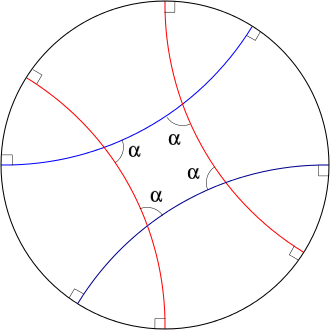
\includegraphics[width=0.4\linewidth]{Quadrato_iperbolico.svg}	\quad
		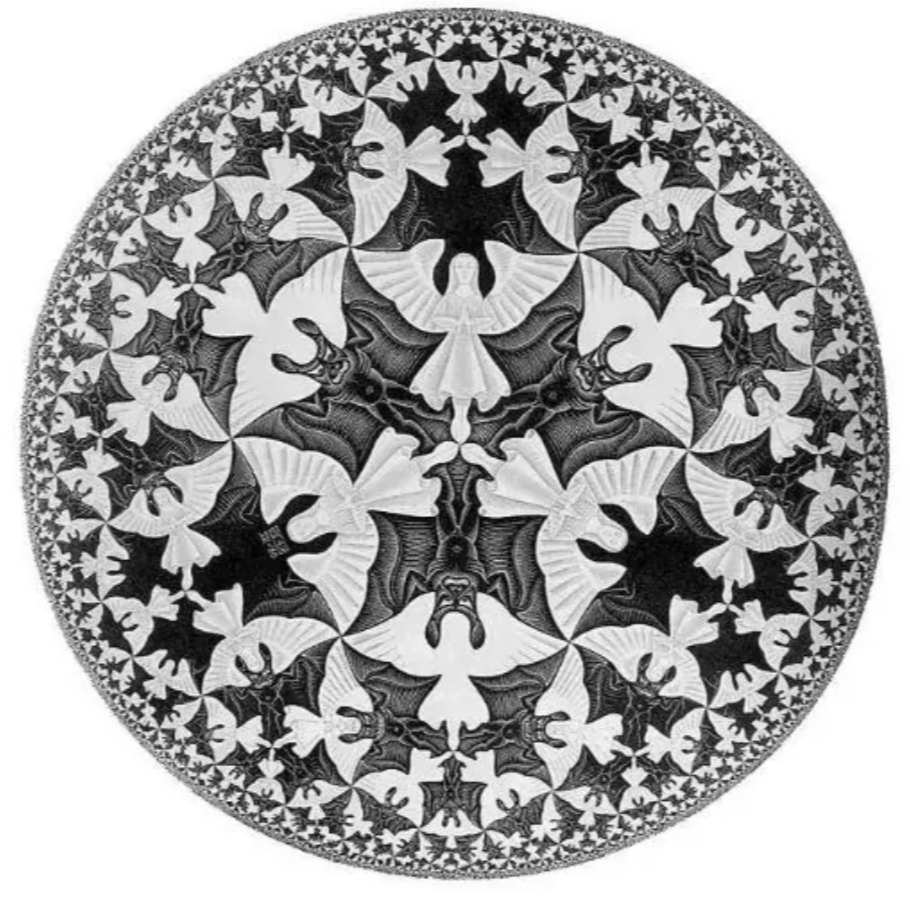
\includegraphics[width=0.4\linewidth]{angeli-demoni}
		\caption{A sinistra: n rosso ed in blu, alcune geodetiche sul disco di Poincacré, la cui intersezione forma un quadrato iperbolico, la cui somma degli angoli interni è minore di \(2\pi\).\\
			A destra: "Angeli e Demoni" di M.C.Esher.}
		\label{fig:quadratoiperbolico}
	\end{figure}
\FloatBarrier
\end{osservazione}
\newpage
\section{Il principio di Maupertuis}
Come visto più volte, se la lagrangiana non dipende esplicitamente dal tempo, le traiettorie soddisfano l'equazione differenziale 
\[H(q, p, t) \equiv \dot{q}p_q-\mathcal{L} = \dot{q}\frac{\partial \mathcal{L}}{\partial \dot{q}}-\mathcal{L} = E = cost.\]
l'energia definisce una superficie sullo spazio delle fasi, dire che le traiettorie, ovvero le curve nello spazio delle fasi, mantengono l'energia costante, equivale a dire che le traiettorie sono vincolate a giacere sulle superfici ad energia costante (l'energia è fissata dalle condizioni iniziali). Ne segue che le traiettorie che soddisfano il principio di minima azione devono soddisfare questo vincolo, conoscendo questa informazione a priori possiamo restringere il dominio del funzionale d'azione: oltre a considerare tutte le traiettorie possibile fra due punti fissati, considero quelle che conservano l'energia. Sia X lo spazio delle configurazioni
\[D = \{q(t), t\in[t_a, t_b], q(t)\in X, q(t_a) = t_a, q(t_b) = q_b, H(p, q) = E\}\] 
restringere il dominio cambia il principio variazionale: se prima cercavamo la funzione che minimizzava il funzionale in un insieme, restringendo l'insieme potrebbe cambiare il minimo (potrebbe darsi che la q(t) cercata non sta nell'intersezione dei due domini). Il principio variazionale resta
\[\delta\int_{t_a}^{t_b}\mathcal{L}dt = 0\]
posso ora invertire la definizione di E e sostituirla al posto della lagrangiana
\[\mathcal{L} = \dot{q}\frac{\partial \mathcal{L}}{\partial \dot{q}}-H\]
per quanto imposto nel dominio, \(H(q, p, t) = E\) dunque
\[\mathcal{L} = \dot{q}\frac{\partial \mathcal{L}}{\partial \dot{q}}-E\]
\[\delta\int_{t_a}^{t_b}\left(\dot{q}\frac{\partial \mathcal{L}}{\partial \dot{q}}-E\right)dt = 0\]
\[\delta\int_{t_a}^{t_b}\dot{q}\frac{\partial \mathcal{L}}{\partial \dot{q}}dt-\delta E(t_b-t_a) = \delta\int_{t_a}^{t_b}\dot{q}\frac{\partial \mathcal{L}}{\partial \dot{q}}dt =  0\]
che è il nuovo principio variazionale, detto principio di Maupertuis, il nuovo funzionale è detto azione ridotta. Vogliamo capire quale sia il significato fisico di questo principio e vogliamo sapere  se ci dice qualcosa di nuovo. 
\begin{osservazione}[Azione ridotta e geometria]
	In questo principio variazionale compare, svolgendo la derivata, due volte l'energia cinetica (se non ci sono potenziali generalizzati il potenziale si annulla), l'energia cinetica dipende dalla metrica e la metrica è la connessione fra interpretazine dinamica e geometrica. Intuiamo che con il principio di Maupertuis ci stiamo avvicinando ad una geometrizzazione più profonda della dinamica.
\end{osservazione}
Vogliamo eliminare il tempo dal principio di Maupertuis per avvicinarci ad una formulazione puramente geometrica della meccanica. Consideriamo una lagrangiana senza potenziali generalizzati, che non dipenda esplicitamente dal tempo: 
\[\mathcal{L} = \frac{1}{2}\dot{q}G\dot{q} -U(q)\]
\[H  = \frac{1}{2}\dot{q}G\dot{q} +U(q) = E\]
\[\dot{q}G\dot{q} = 2E-2U\]
\[\sqrt{\dot{q}G\dot{q}} = \sqrt{2(E-U)}\]
ricordando la definizione di ds, elemento infinitesimo di lunghezza, possiamo scrivere
\[\dot{q}\frac{\partial \mathcal{L}}{\partial \dot{q}} = \dot{q}G\dot{q} = \left(\frac{ds}{dt}\right)^2\]
\[\dot{q}\frac{\partial \mathcal{L}}{\partial \dot{q}}dt = \left(\frac{ds}{dt}\right)ds =  \sqrt{\dot{q}G\dot{q}}ds = \sqrt{2(E-U)}ds\]
sostituendo nel principio di Maupertuis
\[\delta\int_{q_a}^{q_b}\sqrt{2(E-U)}ds =  0\]
ecco eliminato il tempo dal principio variazionale: il parametro con cui esprimiamo le q non è specificato.
\begin{osservazione}[Potenziali e deformazione della metrica]
	Possiamo vedere l'argomento del principio variazionale, in analogia con il problema della ricerca delle geodetiche, come la metrica deformata dal potenziale.
	\[d\sigma \equiv \sqrt{2(E-U(q))}ds\]
	\[\delta\int_{A}^{B}d\sigma = 0\]
	In generale l'influenza del potenziale può essere sempre pensata come deformazione della metrica dello spazio. In questo modo stiamo generalizzando il problema della ricerca delle geodetiche perché prima consideravamo solo particelle libere, ora possiamo considerare anche particele immerse in un campo di forze conservative, deformando la metrica.\\
	Nell'esempio della metrica di Poincaré, abbiamo considerato una metrica euclidea deformata, è un caso matematicamente del tutto analogo a quanto stiamo trattando ora.\\
	Questa è l'idea di base della relatività generale.
\end{osservazione}
Abbiamo già visto la soluzione del problema delle geodetiche, risolvendo questo problema otteniamo le geodetiche, cioè le traiettorie espresse rispetto ad un generico parametro. Se risostituiamo il tempo otteniamo le traiettorie, tornando all'interpretazione dinamica. Il vantaggio è che la soluzione del problema geometrico potrebbe essere più semplice del problema dinamico. 
\subsection{Il problema di Keplero con il principio di Maupertuis}
Scriviamo la lagrangiana del problema di Keplero (m=1) e l'elemento di lunghezza infinitesima in coordinate polari
\[\mathcal{L} = \frac{\dot{r}}{2}+\frac{r^2\dot{\theta}^2}{2}+\frac{k}{r}\]
\[ds = \sqrt{dr^2+r^2d\theta^2}\]
scriviamo il principio di Maupertuis a partire dalla nuova distanza infinitesima, definita in base alla nuova metrica deformata
\[d\sigma  = \sqrt{2(E-U(r))}ds = \sqrt{2\left(E+\frac{k}{r}\right)}\sqrt{dr^2+r^2d\theta^2}=\] \[\sqrt{2\left(E+\frac{k}{r}\right)}\sqrt{\left(\frac{dr}{d\theta}\right)^2+r^2}d\theta = \sqrt{2\left(E+\frac{k}{r}\right)\left[\left(\frac{dr}{d\theta}\right)^2+r^2\right]}d\theta\]
il principio di Maupertuis del problema di Keplero in coordinate polari, che definisce le orbite, è dunque
\[\delta\int_{A}^{B}d\sigma = \delta\int_{\theta_a}^{\theta_b}\sqrt{2\left(E+\frac{k}{r}\right)\left[\left(\frac{dr}{d\theta}\right)^2+r^2\right]}d\theta =0 \]
quando abbiamo studiato il problema di Keplero per la prima volta, abbiamo analogamente abbandonato la dinamica per studiare l'equazione dell'orbita \(r(\theta)\) per poi tornare alla dinamica risostituendo il tempo; il principio di Maupertuis formalizza e rende meccanico questo processo.
Per risolvere questo problema possiamo sfruttare le equazioni di Eulero-Lagrange oppure possiamo cercare di costruire degli integrali del moto considerando l'argomento dell'integrale del funzionale (la "lagrangiana"), la seconda opzione è più semplice.  
\begin{osservazione}[L'energia non è banale]
	Abbiamo visto nel problema delle geodetiche che l'energia diventa un integrale del moto banale se non si scwglie il tempo come parametro. In questo caso la metrica ha una forma tale che anche non scegliendo il tempo come parametro l'energia non è banale.
\end{osservazione}
Scriviamo la definizione di "energia", che chiameremo A per distinguerla da quella ricavata usando come parametro il tempo, per la "lagrangiana" considerata
\[A = \left(r'\frac{\partial}{\partial r'}-1\right)\sqrt{2\left(E+\frac{k}{r}\right)\left[\left(\frac{dr}{d\theta}\right)^2+r^2\right]}=\]
\[\sqrt{\frac{2(E+\frac{k}{r})}{\left(\frac{dr}{d\theta}\right)^2+r^2}}\left(\frac{dr}{d\theta}\right)^2-\sqrt{2\left(E+\frac{k}{r}\right)\left(\frac{dr}{d\theta}\right)^2+r^2}=\]
\[-\sqrt{\frac{2\left(E+\frac{k}{r}\right)}{\left(\frac{dr}{d\theta}\right)^2+r^2}}r^2\]
questa quantità si conserva, è un integrale del moto. Anche E, per come abbiamo costruito il problema, si conserva, è una costante. Per ottenere le equazioni del moto operiamo qualche manipolazione algebrica 
\[\frac{1}{A^2} = \frac{\left(\frac{dr}{d\theta}\right)^2+r^2}{2r^4\left(E+\frac{k}{r}\right)}\]
operiamo la solita sostituzione, utile nello studio di campi centrali: \(u = \frac{1}{r}\); \(\frac{du}{d\theta} = -\frac{1}{r^2}\frac{dr}{d\theta}\)
\[\frac{1}{A^2} = \frac{\left(\frac{du}{d\theta}\right)^2+u^2}{2(E+ku)}\]
\[\frac{E}{A^2} = \frac{1}{2}\left(\frac{du}{d\theta}\right)^2+\frac{u^2}{2}-\frac{k}{A^2}u\]
questa è l'equazione delle orbite: un'equazione differenziale dalla cui risoluzione si ottiene \(r(\theta)\). Osserviamo che la'integrale del moto ricavato formalmente non è altro che il momento angolare, che sappiamo si conserva in tutti i campi centrali; questo fatto non è casuale, è legato alla scelta della variabile: abbiamo scelto $\theta$ e abbiamo ottenuto l'integrale del moto ad esso connesso, ovvero il momento coniugato. Se ad esempio avessimo usato il tempo avremmo riottenuto l'energia come integrale del moto. 

\subsection{Particella relativistica}
la meccanica relativistica è definita nello spaziotempo di Minkowski, uno spazio metrico formato da \(\mathbb{R}^4\) con associata la distanza, detta intervallo relativistico
\[ds^2 = c^2t^2-dx^2\]
dove dx contiene tre componenti spaziali. Questa formulazione geometrica è costruita attorno al fatto che nulla in natura può viaggiare a velocità maggiori di quella della luce: le distanze fisiche infatti sono detti intervalli di tipo tempo, tali per cui \(ds^2>0\), al limite si hanno intervalli di tipo luce, cioè tali che \(ds^2 = 0\), le distanze non fisiche sono dette intervalli di tipo tempo, tali che \(ds^2 < 0\). Un cambio di S.R.I. nello spazio di Minkowski, detta trasformazione di Lorentz, è una rotazione iperbolica che lascia invariato il modulo dei vettori, calcolato con la metrica derivante dalla distanza appena definita. Possiamo rappresentare le trasformazioni di Lorentz come
\begin{align*}
	&\begin{pmatrix}
		ct'\\
		x'
	\end{pmatrix} = 
	\begin{pmatrix}
		\cosh(\alpha)&\sinh(\alpha)\\
		\sinh(\alpha)&\cosh(\alpha)
	\end{pmatrix}
	\begin{pmatrix}
		ct\\
		x
	\end{pmatrix}
\end{align*}
dove definiamo
\[\sinh(\alpha) = \frac{\frac{v}{c}}{\sqrt{1-\frac{v^2}{c^2}}}\]
\[\cosh(\alpha) = \frac{1}{\sqrt{1-\frac{v^2}{c^2}}}\]
la relazione fondamentale della trigonometria iperbolica è 
\[\cosh^2(\alpha)-\sinh^2(\alpha) = 1\]
dunque queste funzioni non conservano il modulo euclideo dei vettori ma il modulo calcolato con la matrice metrica dello spazio di Minkowski, deducibile dalla definizione di \(ds^2\), che è
\begin{align*}
	&g_{ij} =
	\begin{pmatrix}
		1&0&0&0\\
		0&-1&0&0\\
		0&0&-1&0\\
		0&0&0&0&-1
	\end{pmatrix}
\end{align*}
nel limite classico, cioé \(\frac{v}{c}<<1\), cioè \(c\rightarrow \infty\), possiamo sviluppare in serie di taylor al primo ordine, riotteniamo le trasformazioni galileiane.\\
Vogliamo costruire una lagrangiana relativistica della particella libera: deve essere invariante per trasformazioni di Lorentz, dunque posso usare la massa a riposo della particella, la velocità della luce e l'intervallo relativistico, inoltre la lagrangiana deve avere la dimensione di un energia. Unendo gli unici ingredienti che ho, definiamo la lagrangiana come
\[\mathcal{L} = -mcds = -mc^2\sqrt{1-\frac{v^2}{c^2}}dt\]
dove il segno meno è messo per convenzione. Per verificare la correttezza della mia scelta verifico che la lagrangiana di una particella libera, per \(\frac{v}{c}<<1\), deve portare ad una lagrangiana che mi risulti nelle equazioni del moto classiche. La sviluppo in serie di Taylor
\[\mathcal{L} = -mc^2 +mc^2\left(\frac{1}{2}\frac{v^2}{c^2}\right)+...\simeq \frac{1}{2}mv^2\]
che è l'energia cinetica classica, questo giustifica la scelta iniziale del segno meno.
Se inserisco la lagrangiana della particella libera relativistica nel principio di minima azione, posso applicare l'operatore di Lagrange ottenendo
\[\frac{d}{dt}\frac{\partial}{\partial v}(-mc^2\sqrt{1-\frac{v^2}{c^2}}) = \frac{d}{dt}\frac{mc^2}{\sqrt{1-\frac{v^2}{c^2}}}\frac{v}{c^2} = \frac{d}{dt}\frac{mv}{\sqrt{1-\frac{v^2}{c^2}}} = 0\]
da cui segue che le geodetiche relativistiche sono tali da conservare nel tempo la quantità 
\[p = \frac{mv}{\sqrt{1-\frac{v^2}{c^2}}}\]
sono portato a definire questa espressione come la quantità di moto, in analogia al caso classico. Osserviamo che la quantità di moto di una particella che si avvicina alla velocità della luce tende a infinito, dunque non può arrivarci. Capiamo ora anche perché il principio di Newton è meglio formulato in riferimento ai momenti che alle velocità. Possiamo calcolare l'energia usando la solita definizione, essendo la lagrangiana indipendente dal tempo anche nel caso relativistico l'energia è un integrale del moto
\[E = v\frac{\partial}{\partial v}(-mc^2\sqrt{1-\frac{v^2}{c^2}})-(-mc^2\sqrt{1-\frac{v^2}{c^2}}) = \frac{mv^2}{\sqrt{1-\frac{v^2}{c^2}}}+mc^2\sqrt{1+\frac{v^2}{c^2}} = \frac{mc^2}{\sqrt{1-\frac{v^2}{c^2}}}\]
ecco ricavata la celebre equivalenza massa-energia: l'energia di una particella a rioso è pari alla massa per la velocità della luce al quadrato.\\
Per considerare l'interazione fra particelle dobbiamo aggiungere un termine di potenziale che sia invariante per trasformazioni di Lorentz e che abbia la dimensione di un'energia. Risulta che in meccanica analitica relativistica tutti i potenziali sono generalizzati, cioè dipendono anche dalla velocità. 
\begin{osservazione}
	Questo esempio mostra la potenza dell'approccio lagrangiano, che si presta a svariate applicazioni. Un limite della formulazione relativistica appena vista è che risulta impossibile inserire l'interazione gravitazionele. Per farlo si passa alla relatività generale, in cui la metrica relativistica non è più costante ma è deformata dalla presenza di massa.
\end{osservazione}
\newpage
\section{Formulazione Hamiltoniana}
\subsection{Equazioni canoniche del moto}
Hamilton conosceva il principio di Fermat, che nell'ambito dell'ottica geometrica è un principio variazionale secondo il quale un raggio di luce percorre la traiettoria che minimizza il tempo di percorrenza. Hamilton voleva formulare la meccanica a partire dall'ottica geometrica. Si chiede se è possibile trovare una funzione tale che dipenda solo da momenti e coordinate e che produca equazioni del moto al primo ordine e non al secondo ordine, questo è possibile proprio sfruttando i momenti associati alle coordinate al posto delle velocità. Questa scelta comporta il fatto, accettabile, di complicare la geometria dei sistemi fisici in quanto le coordinate sono definite su una varietà e le velocità sullo spazio ad essa tangente mentre i momenti sono definiti sullo spazio cotangente (il duale dello spazio tangente). La geometria della formulazione hamiltoniana è detta simplettica. Osserviamo inoltre che nella formulazione lagrangiana, nonostante usassimo coordinata generalizzata e sua derivata, facevamo spesso uso dei momenti delle coordinate generalizzate per ridurre la dimensione dei problemi: la formulazione naturale della meccanica sembra essere rispetto a coordinate e momenti.\\
Definiamo la funzione di Hamilton a partire dalla definizione di momento associato ad una coordinata
\[\frac{\partial \mathcal{L}}{\partial \dot{q}^k} = p_k\]
Osserviamo che questa relazione è invertibile perché rispetta le condizioni del teorema delle funzioni implicite (del Dini), si veda l'appendice \ref{ap:invertibile}. Ci serve una funzione del tipo $\dot{q} = \dot{q}(q, p, t)$, per trovarla usiamo le trasformazioni di Legendre
\begin{definizione}[Trasformazioni di Legendre]
	Consideriamo una generica \(f = f(x^k, y^k)\), il suo differenziale è
	\[df = \frac{\partial f}{\partial x^k}dx^k+\frac{\partial f}{\partial y^k}dy^k = u_kdx^k+v_kdy^k\]
	vogliamo passare da una descrizione rispetto alle variabili x ed y ad una rispetto le variabili u ed y, esprimendo il differenziale di una nuova funzione g rispetto i differenziali du e dy. Consideriamo la nuova funzione
	\[g = f-u_kx^k\]
	il cui differenziale è
	\[dg = df-u_kdx^k-x^kdu_k\]
	sostituendo in differenziale di f otteniamo
	\[dg = u_kdx^k+v_kdy^k-u_kdx^k-x^kdu_k = v_kdy^k-x^kdu_k\]
	che è ciò che volevamo ottenere.
\end{definizione}
\begin{osservazione}[Le trasformate di Legendre in termodinamica]
	Le trasformate di Legendre si usano per ricavare i potenziali termodinamici: energia interna, potenziale di Helmoltz e Gibbs, entalpia.
\end{osservazione}
Applicando le trasformazioni di Legendre al nostro caso, abbiamo
\[f = \mathcal{L}(q^k, \dot{q}^k, t)\]
\[df =d\mathcal{L} =\frac{\partial \mathcal{L}}{\partial q^k}dq^k+\frac{\partial \mathcal{L}}{\partial\dot{ q}^k}d\dot{q}^k+\frac{\partial \mathcal{L}}{\partial t}dt\]
dunque nel nostro caso
\[x^k = \dot{q}^k\]
\[y^k = q^k\]
\[ u_k = \frac{\partial f}{\partial \dot{q}^k} = p_k\]
\[v_k = \frac{\partial f}{\partial q^k}\]
continuando l'analogia definiamo g
\[g = u_kx^k-f = \dot{q}^k\frac{\partial \mathcal{L}}{\partial \dot{q}^k}-\mathcal{L} = H(q^k, \dot{q}^k, t) \]
si noti che rispetto alle trasformazioni di Legendre in questo passaggio si hanno i segni invertiti, in questo modo otteniamo formalmente la definizione di hamiltoniana. Calcoliamone il differenziale in modo formale
\[dg = dH = d\left(\dot{q}^k\frac{\partial \mathcal{L}}{\partial \dot{q}^k}\right)-d\mathcal{L} = \]
\[\frac{\partial \mathcal{L}}{\partial \dot{q}^k}d\dot{q}^k+\dot{q}^k d\left(\frac{\partial \mathcal{L}}{\partial \dot{q}^k}\right)-\frac{\partial \mathcal{L}}{\partial q^k}dq^k+\frac{\partial \mathcal{L}}{\partial\dot{ q}^k}d\dot{q}^k+\frac{\partial \mathcal{L}}{\partial t}dt\]
sostituendo la definizione di \(p_k\)
\[dH =p_kd\dot{q}^k+\dot{q}^k dp_k-\dot{p}dq^k-p_kd\dot{q}^k-\frac{\partial \mathcal{L}}{\partial t}dt =\dot{q}^k dp_k-\dot{p}_kdq^k-\frac{\partial \mathcal{L}}{\partial t}dt \]
dove abbiamo usato l'equazione di Newton in forma lagrangiana (sotto l'ipotesi che non vi siano potenziali generalizzati)
\[\frac{\partial \mathcal{L}}{\partial q^k} = \dot{p}_k\]
D'altra parte, sappiamo che il differenziale di H deve anche essere uguale a 
\[dH = \frac{\partial H}{\partial q^k}dq^k+\frac{\partial H}{\partial p_k}dp_k+\frac{\partial H}{\partial t}dt\]
confrontando le due espressioni di dH otteniamo le seguenti equazioni
\begin{align*}
	&\begin{cases}
		\dot{q}^k = \dfrac{\partial H}{\partial p_k}\\\\
		\dot{p}_k = -\dfrac{\partial H}{\partial q^k}
	\end{cases}\\
	&\frac{\partial H}{\partial t} = -\frac{\partial \mathcal{L}}{\partial t}
\end{align*}
\begin{osservazione}[Derivate parziali]
	Le derivate parziali non sono oggetti intrinseci ma dipendono dalla funzione alla quale sono applicate: nell'ultima equazione, al primo membro si tengono costanti \(q, p\) mentre al secondo membro \(q, \dot{q}\).
\end{osservazione}
le prime due sono dette equazioni canoniche di Hamilton, ovvero le equazioni del moto sullo spazio delle fasi, che sostituiscono le equazioni del moto di Lagrange. Si osservi come in questa formulazione vi è una simmetria (a meno del segno, che non è importante) fra coordinate e momenti, abbiamo superato la formulazione lagrangiana in quanto ora siamo svincolati dallo scegliere una variabile come derivata dell'altra, non c'è una netta distinzione fra coordinate e momenti. L'ultima equazione stabilisce una relazione fra energia e lagrangiana (ritroviamo che se la lagrangiana è indipendente dal tempo l'energia si conserva).
\begin{osservazione}[Hamiltoniana ed energia]
	Attenzione: l'hamiltoniana è definita usando le variabili q, $\dot{q}$, t. Se al posto di p si usa $\dot{q}$ non si ha propriamente l'hamiltoniana ma l'energia. Il significato fisico di H è quello di energia meccanica perché lo abbiamo ottenuto dalla stessa formula ma matematicamente H non è più un integrale del moto. H è un integrale del moto solo se non dipende dal tempo.
\end{osservazione}
\subsection{Formulazione variazionale}
Come visto, la lagrangiana può essere fatta derivare da un principio variazionale, il principio di minima azione, da cui si ottengono le equazioni del moto. Aver osservato questo fatto è stato utile e abbiamo già sottolineato la potenza dell'approccio variazionale; per questo motivo vogliamo avere una formulazione hamiltoniana fondata su principi variazionali.\\
Partendo dal principio di minima azione,  sostituiamo \(\mathcal{L}\) usando la definizione dell'hamiltoniana
\[\delta\int^{t_a}_{t_b}\mathcal{L}dt = 0\]
\[\delta\int^{t_a}_{t_b}(p\dot{q}-H)dt = 0\]
in entrambe i principi variazionali abbiamo la condizione sulle q di avere gli estremi fissati
\[q(t_a) = q_a\quad q(t_b) = q_b \]
questa condizione, essendo $\dot{q}$ la derivata di \(q\), costituisce indirettamente una condizione anche per $\dot{q}$. Nel nuovo principio variazionale invece non si hanno condizioni sulla variabile p. Notiamo inoltre che il dominio cambia: il primo principio è definito sullo spazio delle configurazioni, il secondo sullo spazio delle fasi, il secondo principio variazionale è dunque un'estensione del primo in quanto è possibile vedere lo spazio delle fasi come una rappresentazione dello spazio delle configurazioni al variare dei momenti (più ampio dello spazio delle configurazioni).\\
Ci chiediamo se questo principio variazionale porti alle equazioni canoniche del moto, analogamente a come il principio variazionale della formulazione lagrangiana ci potava alle equazioni del moto. Per verificarlo operiamo analogamente a quanto fatto nel caso lagrangiano: variamo le coordinate ed i momenti di funzioni piccole a piacere, le sostituiamo nel funzionale ed imponiamo che la variazione sia nulla. La funzione che cerchiamo è una curva nello spazio delle fasi, parametrizzata dal tempo, che minimizzi il funzionale, ovvero
\[\gamma = \gamma(q(t), p(t))\]
dunque il funzionale su cui applicare il principio variazionale è
\[\mathcal{F}[\gamma] = \mathcal{F}[(q, p)] = \int^{t_a}_{t_b}(p\dot{q}-H(q, p, t))dt\]
\[\mathcal{F}[(q+\delta q, p+\delta p)] = \int^{t_a}_{t_b}((p+\delta p)(\dot{q}+\delta\dot{q})-H(q+\delta q, p+\delta p, t))dt\]
sviluppo \(H(q+\delta q, p+\delta p, t)\) in serie di Taylor al primo ordine
\[H(q+\delta q, p+\delta p, t) = H(q, p, t) + \frac{\partial H}{\partial q}\delta q + \frac{\partial H}{\partial p}\delta p+o\left(||(\delta q, \delta p, 0)||\right)\]
sostituisco, trascurando il termine \(\delta p\delta\dot{q}\), essendo un infinitesimo di ordine superiore rispetto a quelli considerati
\[\mathcal{F}[(q+\delta q, p+\delta p)] = \int^{t_a}_{t_b}(p\dot{q}-H(q, p, t))dt+\int^{t_a}_{t_b}\left(\dot{q}\delta p+p\delta\dot{q}- \frac{\partial H}{\partial q}\delta q - \frac{\partial H}{\partial p}\delta p\right)dt\]
dunque la variazione del funzionale è 
\[\delta F[(q, p)] = F[q+\delta q, p+\delta p]-F[(q, p)] = \int^{t_a}_{t_b}\left(\dot{q}\delta p+p\delta\dot{q}- \frac{\partial H}{\partial q}\delta q - \frac{\partial H}{\partial p}\delta p\right)dt\]
perché $\gamma$ sia estremale, è necessario che annulli la variazione del funzionale dunque imponiamo
\[\int^{t_a}_{t_b}\left(\dot{q}\delta p+p\delta\dot{q}- \frac{\partial H}{\partial q}\delta q - \frac{\partial H}{\partial p}\delta p\right)dt = 0\]
integro per parti il secondo termine dell'argomento dell'integrale per eliminare $\delta\dot{q}$, osservando che questa è semplicemente la derivata della funzione arbitrariamente piccola di cui abbiamo incrementato q (la tratto come una funzione qualsiasi). Si ricordi che gli estremi delle coordinate q sono fissati 
\[\int_{t_a}^{t_b}p\delta\dot{q}dt = p\delta q|_{t_a}^{t_b}-\int_{t_a}^{t_b}\dot{p}\delta q dt = -\int_{t_a}^{t_b}\dot{p}\delta q dt\]
\[\int^{t_a}_{t_b}\left(\dot{q}\delta p-\dot{p}\delta q  - \frac{\partial H}{\partial q}\delta q - \frac{\partial H}{\partial p}\delta p\right)dt = 0\]
\[\int^{t_a}_{t_b}\left[\left(\dot{q}-\frac{\partial H}{\partial p}\right)\delta p- \left(\dot{p}+ \frac{\partial H}{\partial q}\right)\delta q\right] dt = 0\]
\[\int^{t_a}_{t_b}\left(\dot{q}-\frac{\partial H}{\partial p}\right)\delta p dt -  \int^{t_a}_{t_b}\left(\dot{p}+ \frac{\partial H}{\partial q}\right)\delta q dt = 0\]
ma $\delta p$ e $\delta q$ sono arbitrari ed indipendenti per ipotesi, dunque questo integrale è nullo se e solo se gli argomenti degli integrali si annullano, otteniamo così le equazioni canoniche del moto
\begin{align*}
	&\begin{cases}
		\dot{q}^k = \dfrac{\partial H}{\partial p_k}\\\\
		\dot{p}_k = -\dfrac{\partial H}{\partial q^k}
	\end{cases}
\end{align*}

\subsection{Trasformazioni canoniche}
Le equazioni di Hamilton sono più potenti rispetto a quelle di Lagrange. In quest'ultima formulazione si riuscivano a ricavare le leggi orarie sostanzialmente effettuando cambi di variabili per semplificare la forma della lagrangiana e ridurre la dimensionalità del sistema, la scelta delle variabili giuste è determinante nella risoluzione dei problemi in formalismo lagrangiano. I cambiamenti di variabili nel formalismo lagrangiano si fanno solo nello spazio delle configurazioni, cioè si cambia la coordinata e si ricava l'altra variabile derivando la coordinata (siamo vincolati ad avere variabili che sono una la derivata dell'altra). Nel formalismo hamiltoniano abbiamo più libertà nel cambiare variabili perché p e q sono indipendenti, dunque possiamo cambiarle entrambi indipendentemente, scambiando eventualmente coordinate e momenti; il cambio di variabili avviene nello spazio delle fasi. L'unica restrizione che abbiamo nel cambiare le variabili nel formalismo hamiltoniano è che queste mantengano la struttura canonica delle equazioni, cioè rispettino le equazioni del moto di Hamilton.
\begin{definizione}[Trasformazione canonica non dipendente dal tempo]\label{def:trasfon-indipendente-tempo}
	La trasformazione (cambio di variabili) \(T(q, p): (q, p)\rightarrow (Q, P)\) non dipendente dal tempo è detta canonica se
	\begin{align*}
		&\forall H(p, q),\ 
		\begin{cases}
			\dot{q} = \dfrac{\partial H}{\partial p}\\
			\dot{p} = -\dfrac{\partial H}{\partial q}
		\end{cases}\Rightarrow 
		\begin{cases}
			\dot{Q} = \dfrac{\partial H'}{\partial P}\\
			\dot{P} = -\dfrac{\partial H'}{\partial Q}
		\end{cases}\\
		&H(q, p) = H'(Q, P)
	\end{align*}
	cioè se il cambio di variabili lascia inalterata la struttura canonica delle equazioni di Hamilton.
\end{definizione} 
Dunque su un cambio di variabili è una trasformazione canonica basterà riscrivere l'Hamiltoniana nelle nuove variabili e, senza ulteriori calcoli, potremo immediatamente scrivere le equazioni del moto. Abbiamo dunque molta più libertà rispetto ai cambi di variabili possibili nel formalismo lagrangiano all'unico prezzo di dover trovare delle trasformazioni canoniche.\\
Per caratterizzare le trasformazioni canoniche vi sono varie strade, una passa per l'utilizzo delle parentesi di Poisson
\begin{definizione}[Parentesi di Poisson]
	Siano \(F(q, p)\), \(G(q, p)\) funzioni regolari definite sullo spazio delle fasi, l'operatore binario parentesi di Poisson è definito come (usando la notazione indiciale, che sottintende una somma per k=1, ..., n)
	\[\{F, G\} = \frac{\partial F}{\partial q^k}\frac{\partial G}{\partial p_k}-\frac{\partial F}{\partial p_k}\frac{\partial G}{\partial q^k}\]
	si osserva facilmente che le parentesi di Poisson sono una forma quadratica bilineare ed antisimmetrica.\\
	Inoltre le parentesi di Poisson sono una derivazione, cioè si comportano come una derivata: vale la regola della derivazione di prodotto
	\[\{F, HG\} = G\{F, H\}+H\{F, G\}\]
	dimostrabile a partire dalla definizione.
\end{definizione} 
Una proprietà interessante è che se faccio le parentesi di Poisson di una coordinata e del suo momento coniugato ottengo l'identità mentre se faccio le parentesi di Poisson di due coordinate o due momenti ottengo sempre zero.
\[\{q^j, p_h\} = \delta^j_{h}\]
\[\{q^j, q^h\} = 0\]
\[\{p_j, p_h\} = 0\]
Un'altra interessante proprietà, nota sotto il nome di identità di Jacobi, è
\[\{F, \{G, H\}\}+\{G, \{H, F\}\}+\{H, \{F, G\}\} = 0\]
dove l'ordine delle funzioni cambia in modo ciclico. Da questa identità apparentemente unicamente matematica, discende ad esempio che se si conservano due componenti del momento angolare, deve conservarsi anche la terza.\\
Sfruttando le parentesi di Poisson possiamo riscrivere le equazioni canoniche
\begin{align*}
		\begin{cases}
		\dot{q}^j = \dfrac{\partial H}{\partial p} = \{q^j, H\}\\
		\dot{p}_j = -\dfrac{\partial H}{\partial q^j} = \{p_j, H\}
	\end{cases}
\end{align*}
In questo modo la simmetria delle equazioni del moto è ancora più evidente in quanto, avendo definito le parentesi di Poisson con un segno negativo fra i due termini, si elimina la differenza di segno fra le due equazioni canoniche. Questa relazione è un caso particolare del fatto che la derivata di una qualsiasi funzione delle coordinate e dei momenti, cioè di una funzione definita sullo spazio delle fasi, è la parentesi di Poisson della funzione con l'hamiltoniana, questo risulta evidente sviluppando la derivata temporale con la regola della catena e usando le equazioni canoniche
\[\frac{d}{dt}F(q, p) = \frac{\partial F}{\partial q^k}\dot{q}^k+\frac{\partial F}{\partial p_k}\dot{p}_k=
 \frac{\partial F}{\partial q^k}\frac{\partial H}{\partial p_k}-\frac{\partial F}{\partial p_k}\frac{\partial H}{\partial q^k} =\{F, H\}\]
Un fatto importante è che se la parentesi di Poisson fra una funzione definita sullo spazio delle fasi e l'hamiltoniana è nulla, allora quella funzione è un'integrale del moto, perché ha derivata temporale nulla (è costante nel tempo). Si osservi che nella formulazione Hamiltoniana gli integrali del moto non sono definiti mediante derivazione temporale, ma usando le parentesi di Poisson, che coinvolgono solamente derivate di F ed H (più in particolare gradienti) rispetto a coordinate e momenti. Ma le condizioni sui gradienti di H ed F, che individuano varietà nello spazio delle fasi, sono condizioni di tipo geometrico.\\
Un altro fatto interessante è che se le parentesi di Poisson fra F ed H sono nulle, allora, essendo questo operatore antisimmetrico, il ruolo di F ed H è lo stesso, posso scambiarli e dire che la funzione H è un'integrale del moto rispetto l'hamiltoniana F. In questo modo andiamo anche oltre il teorema di N\"{o}ther: non solo dal fatto che F è una simmetria di H si conserva F nel sistema definito dall'hamiltoniana H ma anche H è una simmetria di F, dunque si conserva la funzione H nel sistema definito dall'hamiltoniana F. Le simmetrie dei sistemi hamiltoniani non sono più solo simmetrie geometriche nello spazio delle configurazioni (come era nella formulazione lagrangiana) ma sono delle simmetrie nello spazio delle fasi, create da un flusso di fase (e non più solo un flusso, definito nello spazio delle configurazioni), ma il flusso di fase individua un'altro sistema dinamico, dunque il ruolo di simmetria e di sistema dinamico sono intercambiabili!
Trovare le funzioni F ed H tali che \(\{F, H\} = 0\) è molto complesso, abbiamo un'equazione differenziale alle derivate parziali, inoltre vogliamo integrali del moto globali, cioè funzioni che rispettino questa relazione. Poincaré ha dimostrato che trovare le soluzioni di questa equazione è impossibile, trovare F ed H che rispettino questa condizione è un caso del tutto eccezionale.\\\\

Tornando alla ricerca delle trasformazioni canoniche, alla luce di quanto visto, avendo osservato che le equazioni canoniche possono essere scritte con le parentesi di Poisson, una caratterizzazione delle trasformazioni canoniche è quella di conservare le parentesi di Poisson. Posso dunque verificare che una trasformazione sia canonica scrivendo le equazioni canoniche con le parentesi di Poisson nelle vecchie variabili e nelle nuove e vedere se danno lo stesso risultato, per ogni hamiltoniana, cioè per ogni funzione definita sullo spazio delle fasi e regolare. La condizione di canonicità di una trasformazione è dunque
\begin{align*}
	\begin{cases}
		\dot{q} = \{q, H\}_{q, p} = \{q(Q, P), H\}_{(Q, P)}\\
		\dot{p} = \{p, H\}_{q, p} = \{p(Q, P), H\}_{(Q, P)}
	\end{cases}\\
\forall H
\end{align*}
Possiamo semplificare la verifica di canonicità delle trasformazioni grazie al teorema dimostrato in appendice \ref{ap:caratterizzazione}: la verifica di queste condizioni, vedendo H come una generica funzione definita sullo spazio delle fasi, si riduce a verificare che 
\[\{q(Q, P), p(Q, P)\}_{Q, P}=I\]
Un caso in cui è particolarmente semplice verificare che una trasformazione sia canonica è per i sistemi unidimensionali. Lo spazio delle fasi dei sistemi unidimensionali è il piano \(\mathbb{R}^2\), sul piano una trasformazione è canonica se e solo se conserva le aree, cioè se ha determinante dello jacobiano pari a 1. Dimostrarlo è immediato in quanto le parentesi di Poisson di coordinata e momento di un sistema unidimensionale sono sempre
\[\{q, p\} = \frac{\partial q}{\partial q}\frac{\partial p}{\partial p}-\frac{\partial q}{\partial p}\frac{\partial  p}{\partial q}= 1\]
e, data una generica trasformazione 
\[T:(q, p)\rightarrow (q(Q, P), p(Q, P))\]
osserviamo che le parentesi di Poisson di coordinata e momento trasformati sono uguali al determinante dello Jacobiano della trasformazione
\begin{align*}
	&J =
	\begin{pmatrix}
		\dfrac{\partial q(Q, P)}{\partial Q}&\dfrac{\partial q(Q, P)}{\partial P}\\\\
		\dfrac{\partial p(Q, P)}{\partial Q}&\dfrac{\partial p(Q, P)}{\partial P}
	\end{pmatrix}\\
&det(J) = \dfrac{\partial q(Q, P)}{\partial Q}\dfrac{\partial p(Q, P)}{\partial P}
-\dfrac{\partial q(Q, P)}{\partial P}\dfrac{\partial p(Q, P)}{\partial Q} = \{q(Q, P), p(Q, P)\}_{(Q, P)}
\end{align*}
e che quest'ultimo deve essere uguale ad 1 se la trasformazione è canonica.
\begin{esempio}[L'identità]
	Dimostriamo che l'identità è una trasformazione canonica sul piano. Consideriamo un sistema unidimensionale: lo spazio delle fasi è il piano e i suoi vettori sono del tipo \((q, p)\in\mathbb{R}^2\), il determinante dell'identità è pari a 1 dunque è una trasformazione canonica.
\end{esempio}
\begin{esercizio}[Applicazione delle parentesi di Poisson]
	Sia \(L_x = yp_z-zp_y\); \(L_y=zp_x-xp_z\), dimostriamo che le parentesi di Poisson fra due componenti del momento angolare risultano nella terza
	\[\{L_x, L_y\} = \{yp_z-zp_y, zp_x-xp_z\} = \{yp_z, zp_x\}+\{zp_y, xp_z\} =\]
	\[ yp_x\{p_z, z\}+xp_y\{z, p_z\} = xp_y-yp_x = L_z\]
	dove si è usata la linearità delle parentesi di Poisson, il fatto che la parentesi di Poisson di due coordinate e due momenti è nulla, il fatto che le parentesi di Poisson di coordinata e momento sono l'identità e infine l'antisimmetria delle parentesi di Poisson.\\
	Vogliamo ora dimostrare che se \(L_x\) ed \(L_y\) sono integrali del moto anche \(L_z\) lo è. Abbiamo già visto che una funzione è integrale del moto se le parentesi di Poisson fra questa e l'hamiltoniana sono nulle. vogliamo dimostrare che
	\[\{H, L_z\} = 0 \]
	da quanto dimostrato
	\[\{ H, L_z\} = \{H, \{L_x, L_y\}\}\]
	 per l'identità di Jacobi
	\[\{H, \{L_x, L_y\}\} = -\{L_x, \{L_y, H\}\}-\{L_y, \{H, L_x\}\}\]
	\[\{ H, L_z\} = -\{L_x, \{L_y, H\}\}-\{L_y, \{H, L_x\}\}\]
	ma per ipotesi \(L_x\) ed \(L_y\) sono integrali del moto dunque 
	\[\{ H, L_z\} = -\{L_x, 0\}-\{L_y, 0\} = 0\]
	Osservando infine che queste relazioni resta valida ciclando gli indici \(L_i\), ottengo che se due componenti del momento angolare si conservano, si conserva anche la terza.
\end{esercizio}
\begin{esercizio}[Applicazione delle parentesi di Poisson]
	Da quanto dimostrato risulta immediato dimostrare che le parentesi di Poisson fra il modulo quadro di L ed una componente sono nulle. 
	\[\{L^2, L_x\} = \{L_x^2, L_x\}+\{L_y^2, L_x\}+\{L_z^2, L_x\} =  2L_x\{L_x, L_x\}+2L_y\{L_y, L_x\}+2L_z\{L_z, L_x\} =\]
	\[ 2L_y\{L_y, L_x\}+2L_z\{L_z, L_x\}\]
	dove si è usato che le parentesi di Poisson si comportano come le derivate, inoltre le parentesi di Poisson di una stessa quantità è sempre nulla. Uso quanto dimostrato in precedenza facendo attenzione all'ordine degli indici (per non sbagliare i segni)
	\[\{L^2, L_x\} = 2L_yL_z-2L_zL_y = 0\]
	Questo fatto si usa (dimostra Arnold) per costruire il cambio di coordinate globale che ci ha permesso di risolvere il problema della trottola simmetrica libera: abbiamo usato come integrali del moto E, \(L^2\), ed una delle componenti del momento angolare. Senza il fatto che la parentesi di Poisson è nulla potrei costruire solo coordinate locali.
\end{esercizio}
\subsection{Principio variazionale e forme differenziali}
Il nuovo principio variazionale ha una peculiarità che quello precedente non aveva: l'argomento dell'integrale è una 1-forma differenziale
\[(p\dot{q}-H)dt = p\frac{dq}{dt}dt-Hdt = pdq-Hdt\]
il principio variazionale può dunque essere espresso come
\[\delta\mathcal{F}[(q, p)] = \delta\int_{A}^{B}pdq-Hdt = \delta\int_{A}^{B}\omega = 0\]
dove A e B sono punti nello spazio delle fasi. In questa nuova espressione il tempo non ha più un ruolo privilegiato, in quanto non è un parametro ma una variabile come le altre: p è il momento coordinato a q ed H è il momento coordinato a t. Se il principio variazionale è collegato ad una forma differenziale, dimostra l'Arnold, deve essere possibile interpretare geometricamente questo principio, in quanto le 1-forme differenziali sono strettamente legate alla geometria. La geometria è dipende dalla forma differenziale sulla quale è costruita, la geometria costruita sulla 1-forma differenziale
\[\omega  =   p{dq}-Hdt\] 
è detta geometria simplettica ed è la geometria delle soluzioni delle equazioni di Hamilton.\\\\

Possiamo caratterizzare le trasformazioni canoniche avvalendoci delle 1-forme differenziali. Ci chiediamo come agisca sulla 1-forma differenziale una trasformazione canonica \(T:(q, p)\rightarrow(q(Q, P), p(Q, P))\). Se la trasformazione è canonica le equazioni canoniche non cambiano, le equazioni canoniche discendono dal principio variazionale in cui è coinvolta la 1-forma differenziale. Sappiamo che, essendo il principio variazionale definito mediante un integrale con gli estremi fissi, l'argomento dell'integrale è sempre definito a meno di un differenziale esatto di una funzione
\[\delta\int_{A}^{B}\omega= \delta\int_{A}^{B}p{dq}-Hdt= \delta\int_{A}^{B} p(Q, P){dq(Q, P)}-Hdt\]
questa uguaglianza è valida se
\[\delta\int_{A}^{B} p(Q, P){dq(Q, P)}-H(Q, P)dt = \delta\int_{A}^{B} PdQ-H'(Q, P)dt+dF\]
dove in generale l'hamiltoniana può essere diversa da quella iniziale a seguito del cambio di variabili. In questo modo
\[\delta\int_{A}^{B}p{dq}-Hdt = \delta\int_{A}^{B} PdQ-H'dt+\delta (F(B)-F(A))= \delta\int_{A}^{B} PdQ-H'dt\]
le equazioni canoniche derivanti dal principio variazionale al primo membro sono le stesse di quelle derivanti da quello a secondo membro, dunque la struttura canonica è preservata. Abbiamo dimostrato che una trasformazione canonica agisce sulla 1-forma differenziale in modo da modificarla di un differenziale esatto.\\ 
Possiamo sfruttare questi fatti per svolgere utili considerazioni sulle trasformazioni canoniche: 
\[\omega = pdq-Hdt = PdQ-H'dt +dF\]
consideriamo dapprima il caso in cui la trasformazione non dipende dal tempo, ne segue che
\[dF =  pdq-PdQ\]
ma allora \(F=F(q, Q)\) dunque
\[ pdq-PdQ-Hdt+H'dt = \frac{\partial F}{\partial q}dq+\frac{\partial F}{\partial Q}dQ\]
da cui
\begin{align*}
	&\begin{cases}
		\dfrac{\partial F}{\partial q} = p\\\\
		\dfrac{\partial F}{\partial Q} = -P
	\end{cases}\\
&H = H'
\end{align*}
queste relazioni definiscono in forma implicita il cambio di variabili dato dalla trasformazione canonica, si noti che se F non dipende dal tempo l'hamiltoniana non cambia a seguito del cambio di variabili.\\
 Se per ipotesi F è invertibile, cioè, per il teorema della funzione implicita
\[\frac{\partial^2 F}{\partial q\partial Q}\neq 0\]
allora posso invertire le relazioni precedenti e ricavare \(F(q, Q)\), da cui ottengo dF, da cui posso definire la trasformazione canonica. F è detta funzione generatrice del primo tipo della trasformazione canonica T.\\
La libertà che ho nello scegliere F è enorme e questo può semplificare la risoluzione dei problemi: ad esempio posso modificare F come segue
\[PdQ-Hdt +dF= PdQ-Hdt +d(QP)-d(QP)+dF=\]
\[PdQ-PdQ-QdP-Hdt+d(F+QP) = -QdP-Hdt+dG = pdq-Hdt=\]
ma allora \(G = G(q, P)\)
\[dG = pdq+QdP\]
sviluppando il differenziale di G e confrontando i due membri otteniamo
\[-QdP-Hdt+\frac{\partial G}{\partial q}dq+\frac{\partial G}{\partial P}dP = pdq-Hdt\]

\begin{align*}
	\begin{cases}
		\dfrac{\partial G}{\partial q} = p\\\\
		\dfrac{\partial G}{\partial P} = Q
	\end{cases}
\end{align*}
G è detta generatrice del secondo tipo della trasformazione canonica T.\\
 L'introduzione delle generatrici del secondo tipo è necessaria in quanto è facile verificare che le generatrici del primo tipo da sole non generano tutte le possibili trasformazioni canoniche. Ad esempio quelle del primo tipo non possono esprimere l'identità mentre quelle del secondo sì.\\
Un'altra considerazione interessante è che l'insieme delle trasformazioni canoniche formano un gruppo rispetto all'operazione di composizione. Questo è abbastanza ovvio perché se faccio una trasformazione canonica conservo le equazioni di Hamilton, se opero nuovamente una trasformazione le equazioni di Hamilton continuano ad essere conservate.
\subsection{Equazione di Hamilton-Jacobi: trasformazioni canoniche dipendenti dal tempo}
Fin ora abbiamo considerato trasformazioni canoniche non dipendenti dal tempo, tuttavia la formulazione hamiltoniana permette di tener conto anche di quelle dipendenti dal tempo in modo elegante e questo è il suo principale punto di forza. Sia F una generatrice di trasformazioni canoniche del primo tipo dipendente dal tempo, dunque \(F = F(q, Q, t)\) invertibile. 
\[pdq-Hdt = PdQ-H'dt+dF\]
\[PdQ-H'dt+\frac{\partial F}{\partial q}dq+\frac{\partial F}{\partial Q}dQ+\frac{\partial F}{\partial t}dt = pdq-Hdt\]
da cui segue 
\begin{align*}
	\begin{cases}
		\dfrac{\partial F}{\partial q} = -p\\\\
		\dfrac{\partial F}{\partial Q} = P\\\\
		H' = H+\frac{\partial F}{\partial t}
	\end{cases}
\end{align*}
la struttura canonica resta sempre inalterata in quanto dF è sempre un differenziale esatto ma l'hamiltoniana cambia. Possiamo dunque definire le trasformazioni canoniche in modo più generale, considerando anche quelle dipendenti dal tempo
\begin{definizione}[Trasformazioni canoniche]
	Una trasformazione \(T(q, p, t): (q, p)\rightarrow (Q, P)\) è detta canonica se
	\begin{align*}
		&\forall H(p, q),\ 
		\begin{cases}
			\dot{q} = \dfrac{\partial H}{\partial p}\\
			\dot{p} = -\dfrac{\partial H}{\partial q}
		\end{cases}\Rightarrow 
		\begin{cases}
			\dot{Q} = \dfrac{\partial H'}{\partial P}\\
			\dot{P} = -\dfrac{\partial H'}{\partial Q}
		\end{cases}\\
		& H' = H +\frac{\partial F}{\partial t}
	\end{align*}
	dove F è una funzione tale per cui dF è un differenziale esatto.
\end{definizione}
Osservando che l'hamiltoniana cambia se la trasformazione è dipendente dal tempo, Hamilton ha l'idea di cercare una \(F(q, Q, t)\) che semplifichi al massimo il problema, cioè tale che la nuova hamiltoniana sia nulla, in questo modo le equazioni del moto che ne discendono diventano banali
\begin{align*}
&H' = 0 \Rightarrow
\begin{cases}
	\dot{P} = 0\\
	\dot{Q} = 0
\end{cases}
\end{align*}
la cui risoluzione è triviale: P e Q sono integrali del moto. In questo modo sposto la risoluzione dei problemi meccanici alla ricerca di un opportuno cambio di coordinate e quindi alla ricerca di un'opportuna trasformazione canonica.\\
L'equazione da risolvere per trovare le F che soddisfano questa richiesta, con cui è possibile costruire le trasformazioni canoniche adeguate, è dunque
\[H' = H+\frac{\partial F}{\partial t}=0\]
\[H(q, p, t)+\frac{\partial F}{\partial t}(q, Q, t)=0\]
ma così l'equazione non è bilanciata perché da un lato ho p e dall'altro ho Q: sostituisco 
\[p = \frac{\partial F}{\partial q}\]
\[H(q, \frac{\partial F}{\partial q}, t)+frac{\partial F}{\partial t}(q, Q, t)=0\]
questa è detta equazione di Hamilton-Jacobi.\\
\'E una brutta bestia perché è un'equazione differenziale alle derivate parziali non lineare, la soluzione inoltre deve sottostare alla condizione di essere invertibile (vista sopra) il che complica ulteriormente le cose (altrimenti non potremmo trovare la trasformazione canonica). Nonostante la difficoltà, l'equazione di Hamilton-Jacobi è l'equazione fondamentale della dinamica, permette di integrare sistemi che non sarebbero integrabili (o riconosciuti come tali) in formulazione lagrangiana, è il metodo più potente per studiare sistemi meccanici classici e generazioni di ricercatori hanno passato la vita a studiarla. Si risolve solitamente con metodi numerici.
\subsection{Variabili azione angolo generalizzate}
Vogliamo generalizzare quanto visto per l'oscillatore armonico 1-D qualsiasi curva chiusa sullo spazio delle fasi, continuando a limitarci ai sistemi 1-D, alla luce delle conoscenze sulla formulazione hamiltoniana. L'idea di base è di sfruttare l'area delle curve chiuse come coordinata, l'area di una curva chiusa definita dalla funzione p(q), fissato un valore di \(H(q, p)\), è
\[A(E) = \oint_{H = E}p(q)dq\]
la variabile d'azione è, analogamente a quanto fatto nel caso dell'oscillatore
\[I = \frac{1}{2\pi}\oint_{H = E}p(q)dq\]
vogliamo trovare la trasformazione canonica \(T(q, p)\rightarrow(\theta, I)\). Osservando che l'azione è funzione dell'energia, se questa è invertibile possiamo scrivere \(E = E(I)\), in questo modo la funzione
\[G(q, I) = \int_{H = E(I)}^qpdq\]
è una funzione che dipende sia da q che da I. Se consideriamo G una trasformazione canonica del secondo tipo e vediamo I come un momento e \(\theta\) come una coordinata, tale funzione può definire implicitamente una trasformazione canonica T del tipo cercato, se rispetta le seguenti condizioni
\begin{align*}
	\frac{\partial G}{\partial q}|_{I} =p\\
	\frac{\partial G}{\partial I}|_{q} = \theta
\end{align*}
la prima equazione è evidentemente soddisfatta, poiché fissata I la derivata dell'integrale lasia solo p. Dalla seconda equazione risulta che, una volta scelta I, la scelta di $\theta$ risulta vincolata. Osservando che in questa equazione q resta costante, G è solamente funzione di E, che come osservato prima, può essere espressa come funzione di I, invertendone la definizione
\[G = G(E(I))\]
usando la regola della catena
\[\frac{\partial G}{\partial I} = \frac{\partial E}{\partial I}\frac{d G}{d E} = \frac{\partial E}{\partial I}\frac{d}{dE}\int_{H = E(I)}^qpdq\]
ma tenendo fissa q, il momento è funzione della sola E dunque
\[\frac{\partial G}{\partial I} = \frac{\partial E}{\partial I}\int_{H = E(I)}^q\frac{\partial p}{\partial E}dq = \theta\]
Possiamo trovare una relazione fra le variabili azione angolo ed il tempo: dalle equazioni di Hamilton
\[\dot{q} = \frac{\partial H}{\partial p}\]
\[\Rightarrow \frac{1}{\dot{q}} = \frac{1}{\frac{\partial H}{\partial p}} = \frac{\partial p}{\partial E}\]
dove nell'ultimo passaggio si è sostituito E con H. Moltiplicando per dq primo ed ultimo membro ed integrando otteniamo 
\begin{align*}
 \frac{dq}{\dot{q}}= dt(q, E) = \frac{\partial p}{\partial E}dq
\end{align*}
possiamo utilizzare questa relazione per ottenere
\[\frac{\partial I}{\partial E} = \frac{\partial}{\partial E}\frac{1}{2\pi}\oint_{H = E}pdq = \frac{1}{2\pi}\oint_{H = E}\frac{\partial p}{\partial E}dq = \frac{1}{2\pi}\oint_{H = E}dt = \frac{T(E)}{2\pi}\]
Chiaramente, se le orbite sono illimitate la curva non è regolare, se invece lo sono (\(T(E)<\infty\)), invertendo la relazione 
\[\frac{\partial E}{\partial I} = \frac{2\pi}{T(E)} = \omega (I)\]
dove $\omega$ è la frequenza d'oscillazione delle orbite. Infine, la variabile angolo può essere scritta come
\[\theta =  \frac{\partial E}{\partial I}\int_{H = E(I)}^q\frac{\partial p}{\partial E}dq = \omega (I)\int_{H = E(I)}^qdt = \omega(I)t \]
La trasformazione è dunque canonica per costruzione, le equazioni del moto sono
\begin{align*}
	&\dot{\theta} = \frac{\partial H}{\partial I}=\omega(I) \\
	&\dot{I} = 0
\end{align*}
La cui risoluzione banale è
\begin{align*}
	\theta(t) = \theta_0 +\omega(I)t\\I(t) = I_0
\end{align*}

\newpage
\section{Corpi rigidi}
Fin ora si è parlato dello studio della dinamica di particelle, ora tratteremo la dinamica di corpi macroscopici, formati da insiemi enormi di particelle, con le dovute ipotesi semplificative. In particolare tratteremo un'astrazione dei corpi reali, ma che modellizza bene una grande classe di essi: i corpi rigidi. La condizione di rigidità di un sistema di particelle è, come visto
\[(r_i-r_j)^2-c_{ij^2} = 0\]
che è un vincolo olonomo, dunque i gradi di libertà si riducono se scegliamo le coordinate opportune, dunque l'apparente enorme complessità che scaturirebbe da un'insieme tanto grande di particelle è ridotta.
\subsection{Scegliere le coordinate}
I gradi di libertà per ogni corpo rigido sono dunque 6 in tutto: tre per rappresentare, rispetto ad un S.R.I. esterno, la posizione dell'origine di un S.R. solidale al corpo e tre per specificare l'orientamento degli assi del S.R. solidale al corpo, rispetto al S.R.I. esterno.\\
Per semplicità in seguito considereremo sempre corpi rigidi con un punto fisso, cioè un punto in quiete o in moto rettilineo uniforme, il cui stato dinamico non è coinvolto nell'evoluzione temporale del sistema. Con questa assunzione i gradi di libertà si riducono a 3, in quanto possiamo scegliere il S.R.I. ed il S.R. con origine nel punto fisso, le coordinate del centro del S.R. saranno dunque sempre fisse all'origine. Gli unici tre gradi di libertà rimasti sono quelli che individuano l'orientamento degli assi solidali al corpo rigido rispetto al S.R.I.\\
Il teorema di Eulero dimostra (si veda appendice \ref{ap:teorema-Eulero}) che ogni spostamento di un corpo rigido con un punto fisso è una rotazione attorno ad un certo asse, passante per il punto fisso. Alla luce di ciò, possiamo osservare come il vincolo di corpo rigido definisca una varietà 6-dimensionale
\[\mathcal{M} = \mathbb{R}^3\times SO(3)\]
dove \(SO(3)\) è lo spazio speciale ortogonale, che rappresenta le rotazioni tridimensionali.
Alla luce di ciò osserviamo come l'ipotesi dell'esistenza di un punto fisso non è restrittiva nel caso del corpo rigido libero, che può sempre essere visto come un copro rigido con un punto fisso. Se infatti facessimo cadere l'ipotesi dell'esistenza di un punto fisso, se il corpo rigido è libero, avremmo nel caso più generale una traslazione del corpo composta ad una rotazione. La velocità di ogni punto del corpo rigido è esprimibile, nel sistema di riferimento centrato nel centro di massa del corpo rigido, come
\[v_{s.r.i.} =v_{c.m.}+\omega\times x \]
dove la velocità di traslazione di ogni punto deve essere la stessa di quella del centro di massa per la condizione di rigidità.  Possiamo allora scrivere l'energia cinetica come
\[T = \frac{1}{2}\int\rho(v_{c.m.}+\omega\times x)^2dx = \frac{1}{2}Mv_{c.m.}^2+\frac{1}{2}v_{c.m.}^2\int\rho(\omega\times x)dx+\frac{1}{2}\int\rho (\omega\times x)^2 dx\]
il termine del doppio prodotto è nullo poiché, ciclando i termini
\[\frac{1}{2}v_{c.m.}^2\int\rho(\omega\times x)dx = \frac{1}{2}\int \rho x (\omega\times v_{c.m.})dx  = (\omega\times v_{c.m.})\int \rho x dx= 0 \]
\[T = \frac{1}{2}Mv_{c.m.}^2 + \frac{1}{2}\int\rho(v_{c.m.}+\omega\times x)^2dx\]
che è il teorema di K\"{o}nig, molto utile nella risoluzione di problemi pratici riguardanti i corpi liberi, e che permette di ridurre il problema del corpo rigido libero ad uno di un corpo rigido con un punto fisso.\\
Tornando al problema della scelta delle coordinate, dal momento che il S.R. solidale al corpo rigido è un S.R. rotante, per esprimere l'orientamento degli assi rotati servono delle coordinate adattate ad SO(3), ne esistono varie ma usiamo quelle più note: gli angoli di Eulero. L'idea è di partire dalle coordinate del S.R.I. ed effettuare tre rotazioni attorno a tre assi per passare a quelle del S.R., le rotazioni non sono commutative dunque è importante l'ordine in cui sono fatte
 \begin{enumerate}
 	\item Rotazione di un angolo $\phi$ attorno l'asse z con una matrice di rotazione B
 	\[(x, y, z)\rightarrow (\xi, \eta, \zeta)\]
 	con \(\zeta = z\). L'asse $\xi$ è detto linea dei nodi.
 	\item Rotazione di un angolo $\theta$ attorno l'asse $\xi$ con una matrice di rotazione C
 	\[(\xi, \eta, \zeta)\rightarrow (\xi', \eta', \zeta')\]
 	con \(\xi' = \xi\)
 	\item Rotazione di un angolo $\psi$ attorno l'asse $\zeta'$ con una matrice di rotazione D
 	\[(\xi', \eta', \zeta')\rightarrow (x', y', z')\]
 	con \(\zeta' = z'\)
 	che sono gli assi cercati.
 \end{enumerate}
\begin{osservazione}
	Per mantenere l'iniettività di queste coordinate $\theta$ deve essere un'angolo polare: varia nell'intervallo \(0, \pi\). Ci aspettiamo che per $\theta = 0, \pi$ le nostre coordinate degenerano.
\end{osservazione}
La matrice di trasformazione A che porta dalle coordinate del S.R.I. a quelle del S.R. è data dalla composizione delle matrici di rotazione
\[A =  DCB\]
\[x'=Ax=DCBx\]
dove, le matrici di rotazione sono
\begin{align*}
	&B =
	\begin{pmatrix}
		\cos\phi&\sin\phi&0\\
		-\sin\phi&\cos\phi&0\\
		0&0&1
	\end{pmatrix}\\
	&C =
	\begin{pmatrix}
		1&0&0\\
		0&\cos\theta&\sin\theta\\
		0&-\sin\theta&\cos\theta
	\end{pmatrix}\\
	&D =
	\begin{pmatrix}
		\cos\psi&\sin\psi&0\\
		-\sin\psi&\cos\psi&0\\
		0&0&1
	\end{pmatrix}
\end{align*}
In definitiva, le coordinate che descrivono un corpo rigido con un punto fisso possono essere espresse dai tre angoli di rotazione (\(\phi, \theta, \psi\)).\\
Le rotazioni sono avvenute lungo gli assi (\(z, \xi', z'\)); la velocità angolare delle tre rotazioni rispetto a questi assi è dunque
\begin{align*}
	\omega_z = (0, 0, \dot{\phi})\\
	\omega_{\xi'} = ( \dot{\theta},0,  0)\\
	\omega_{z'} = (0, 0, \dot{\psi})\\
\end{align*}
vogliamo esprimere queste velocità angolari rispetto al S.R. rotante: \(\omega = (\omega_{z})_{s.r.}+(\omega_{\xi'})_{s.r.}+ (\omega_{z'})_{s.r.}\). Per arrivare agli assi del S.R. a partire da questi assi sfalsati dobbiamo applicare le matrici di rotazione.\\
Cominciamo osservando che, visto che la terza rotazione avviene attorno l'asse z', non ha bisogno di essere trasformata
\[(\omega_{z'})_{s.r.} = (0, 0, \dot{\psi})\]
Per passare da $\omega_{\xi'}$ a \((\omega_{\xi'})_{s.r.}\) dobbiamo ruotare attorno l'asse $z'$: applichiamo \(D\)
\begin{align*}
	&\omega_{y'} = D\omega_{\xi'}=
	\begin{pmatrix}
		\cos\psi&\sin\psi&0\\
		-\sin\psi&\cos\psi&0\\
		0&0&1
	\end{pmatrix}
\begin{pmatrix}
	\dot{\theta}\\
		0\\
		0
\end{pmatrix} =
\begin{pmatrix}
	\dot{\theta}\cos\psi\\
	-\dot{\theta}\sin\psi\\
	0
\end{pmatrix}
\end{align*}
Per passare da $\omega_{z}$ a  $(\omega_{z})_{s.r.}$ dobbiamo effettuare la rotazione completa A = DCB, risparmiamo i conti e scriviamo direttamente il risultato
\begin{align*}
	&\omega_{x'} = A\omega_{\zeta}=
	DCB	
	\begin{pmatrix}
		0\\
		0\\
		\dot{\phi}
	\end{pmatrix}=
	\begin{pmatrix}
		\dot{\phi}\sin\theta\sin\psi\\
		\dot{\phi}\sin\theta\cos\psi\\
		\dot{\phi}\cos\theta
	\end{pmatrix}
\end{align*}
la velocità angolare della rotazione A è la somma di queste componenti dunque
\begin{align*}
&\omega = (\omega_{z})_{s.r.}+(\omega_{\xi'})_{s.r.}+ (\omega_{z'})_{s.r.} = 
\begin{pmatrix}
	\dot{\theta}\cos\psi+\dot{\phi}\sin\theta\sin\psi\\
	-\dot{\theta}\sin\psi+\dot{\phi}\sin\theta\cos\psi\\
	\dot{\phi}\cos\theta+\dot{\psi}
\end{pmatrix}=
\begin{pmatrix}
\omega_{x'}\\
\omega_{y'}\\
\omega_{z'}
\end{pmatrix}
\end{align*}
queste espressioni torneranno utili in seguito.
 \subsection{Energia cinetica e tensore d'inerzia}
L'obiettivo ultimo di questa sezione è quello di studiare le equazioni del moto del corpo rigido con un punto fisso, per farlo vogliamo usare il formalismo lagrangiano: scriviamo innanzitutto l'energia cinetica del corpo rigido. A priori questo è un sistema di particelle e l'energia cinetica del sistema è la somma delle energie cinetiche delle particelle
\[T = \sum_i \frac{m_i}{2}v_i^2\]
le velocità che compaiono in questa espressione sono espresse rispetto ad un sistema di riferimento inerziale, abbiamo già ricavato la relazione fra velocità in un S.R.I. e velocità in un S.R. rotante
\[v = v'+\omega\times x\]
dove v è la velocità rispetto al S.R.I. e v' rispetto al S.R. rotante. Nel nostro caso la velocità relativa al S.R. rotante è nulla perché questo è per ipotesi solidale al corpo e il corpo è rigido, ne segue che
\[v = \omega\times x\]
\[T = \sum_i \frac{m_i}{2}(\omega\times x_i)^2\]
sviluppiamo il quadrato del prodotto vettoriale: osserviamo che in coordiate cartesiane
\[(\omega\times x_i)^2 = (|\omega| |x_i|\sin\theta)^2 = |\omega|^2|x_i|^2(1-\cos^2\theta) =\]
\[|\omega|^2|x_i|^2-(\omega x_i\cos\theta)^2 = |\omega|^2|x_i|^2-(\omega\cdot x_i)^2  \]
\[T = \sum_i \frac{m_i}{2}(|\omega|^2|x_i|^2-(\omega\cdot x_i)^2)\]
passiamo in notazione indiciale: omettiamo l'indice che individua l'iesima particella ma lasceremo il simbolo di sommatoria per ricordare che stiamo parlando di una somma su tutte le particelle del corpo rigido.  Per non appesantire la notazione ometteremo i valori assoluti
\[T = \sum \frac{m}{2}(\omega^k\omega_k x^lx_l-\omega^j x_j\omega^i x_i) =\]
\[ \sum \frac{m}{2}(\omega^k\delta_{kh}\omega^h x^lx_l-\omega^k\delta^{j}_k x_j\omega^h\delta^{i}_h x_i) =  \]
\[\frac{\omega^k\omega^h}{2} \sum m( x^lx_l\delta_{kh}- x_j\delta^{j}_k\delta^{i}_h x_i) = \]
\[\frac{\omega^k\omega^h}{2} \sum m( x^lx_l\delta_{kh}- x_kx_h)\]
Possiamo definire il tensore d'inerzia
\[I_{kh} \equiv \sum m( x^lx_l\delta_{kh}- x_kx_h) \]
ed esprimere l'energia cinetica come una forma quadratica con associato il tensore d'inerzia al posto della metrica
\[T=\frac{\omega_kI_{kh}\omega_h}{2} = \frac{\omega I\omega}{2} \]
Dalla definizione risulta chiaro che l'inerzia è una grandezza additiva: se un sistema è formato da più parti la somma dei tensori d'inerzia delle parti è il tensore d'inerzia totale.
Un'altra osservazione possibile a partire dalla definizione è che l'inversione degli indici lascia immutato il tensore d'inerzia: è un tensore simmetrico. Essendo tale può sempre essere diagonalizzato per il teorema spettrale dunque possiamo sempre trovare un sistema di riferimento, detto sistema degli assi principali, il tensore d'inerzia è diagonale, le componenti del tensore d'inerzia lungo gli assi principali sono detti momenti principali d'inerzia. Nel sistema degli assi principali l'energia cinetica si riduce a
\[T = \frac{1}{2}(I_1\omega_1^2+I_2\omega_2^2+I_3\omega_3^2)\] 
\begin{definizione}[Trottole]
	I corpi possono essere classificati in base agli autovalori del loro tensore d'inerzia
	\begin{itemize}
		\item Trottola asimmetrica: ha tutti gli momenti principali d'inerzia diversi
		\item Trottola simmetrica: ha due momenti principali d'inerzia uguali
		\item Trottola sferica: ha tutti gli momenti principali d'inerzia uguali
	\end{itemize}
\end{definizione}
Nel caso in cui il corpo rigido è formato da una distribuzione continua di particelle bisognerà passare al continuo usando la densità, esprimendo la massa della porzione infinitesima di cormo come \(dm = \rho(x)dV\)
\[I_{kh} \equiv \int_V ( x^lx_l\delta_{kh}- x_kx_h)\rho(x)dV \]
\begin{osservazione}
	Possiamo vedere il tensore d'inerzia rispetto ad un asse come la somma su tutti i punti delle distanze dall'asse al quadrato per la massa del punto. 
	\[I_{asse} = \sum_im_i d_i^2\]
	Questa definizione è equivalente a quella da noi ricavata: possiamo vedere la distanza di un punto dall'asse come il seno del modulo del vettore posizione del punto
	\[d_i = r_i\sin\theta = r_i\times \hat{n}\]
	dove $\theta$ è l'angolo compreso fra l'asse di rotazione e il vettore posizione del punto e $\hat{n}$ è la direzione dell'asse di rotazione.
	\[I_{asse} = \sum_im_i (r_i\times\hat{n})(r_i\times\hat{n})\]
	usando le proprietà del prodotto vettoriale
	\[I_{asse} = \sum_im_i r_i\cdot(\hat{n}\times(r_i\times\hat{n}))\]
	usando il BAC-CAB osservando che \(\hat{n}\cdot\hat{n} = 1\)
	\[I_{asse} = \sum_im_i r_i\cdot(r_i-\hat{n}\cdot(r_i\cdot\hat{n})) = \sum_im_i (r_i^2-(r_i\cdot\hat{n})^2)\]
	che è la nostra definizione.
\end{osservazione}
Infine osserviamo che
\[T = \sum_i \frac{m_i}{2}(\omega\times x_i)^2 = T = \sum_i \frac{m_i}{2}v_i(\omega\times x_i) = 
\sum_i \frac{m_i}{2}\omega(x_i\times v_i) =  \frac{1}{2}\omega\sum_i(x_i\times m_iv_i) = \frac{1}{2}\omega L\]
confrontandola con quanto ottenuto con il tensore d'inerzia otteniamo
\[\frac{1}{2}\omega L = \frac{\omega I\omega}{2}\]
\[L = I\omega\]
notiamo inoltre che il momento angolare è covariante, proprio come il momento della quantità di moto infatti 
\[L_h = I_{kh}\omega^k\]
Da queste relazioni notiamo che in generale momento angolare e velocità angolare non sono paralleli, nel sistema degli assi principali abbiamo
\[(L_x, L_y, L_z) = (I_x\omega_x, I_y\omega_y, I_z\omega_z)\]
Solo se la rotazione avviene su uno degli assi principali si ha \(L \parallel \omega \) infatti
\[(L_x, L_y, L_z) = (I_x\omega_x, 0, 0)\]
In pratica considereremo sempre oggetti con delle simmetrie e calcoleremo sempre i momenti principali d'inerzia rispetto gli assi principali.\\
Nel calcolare i momenti d'inerzia dei corpi rigidi risulta utile il seguente teorema
\begin{teorema}[Degli assi principali o di Steiner]
	Il momento d'inerzia (\(I'\)) rispetto ad un asse parallelo ad un'asse passante per il centro di massa è uguale al momento d'inerzia rispetto l'asse passante per il centro di massa (\(I_{c.m.}\)) più la massa totale M del corpo moltiplicata per la distanza d fra i due assi
	\[I' = I_{c.m.} + Md^2\] 
\end{teorema}
In conclusione, possiamo scrivere l'energia nel sistema degli assi principali sostituendo le componenti di $\omega$ espresse con gli angoli di Eulero ottenute in precedenza nell'espressione di T ricavata.
\[T = \frac{1}{2}\left[I_1(\dot{\theta}\cos\psi+\dot{\phi}\sin\theta\sin\psi)^2+
I_2(-\dot{\theta}\sin\psi+\dot{\phi}\sin\theta\cos\psi)^2+\\
I_3(\dot{\phi}\cos\theta+\dot{\psi})^2\right]\]
\begin{esercizio}
	Si consideri una lamina omogenea quadrata di lato 2l e massa m vincolata a ruotare attorno
	ad un asse orizzontale passante per la diagonale. Ad uno dei vertici non appartenenti
	alla diagonale è vincolata un'asta omogenea di massa m e lunghezza 2l che oscilla nel
	piano verticale contenente la lamina; il tutto è soggetto alla forza peso. Detti $\phi$ l'angolo di rotazione della lamina e $\theta$ l'angolo di oscillazione dell'asta.\\
	1) Scrivere la Lagrangiana del sistema;\\

	La risoluzione dell'esercizio si basa sulla considerazione che l'energia cinetica e il momento d'inerzia sono additivi, dunque consideriamo separatamente i due corpi rigidi. Cominciando dalla lamina, il momento d'inerzia è calcolabile rispetto a qualsiasi asse di simmetria
	\[I = \rho\iint d^2 ds = \frac{m}{4l^2}\iint_{-l}^{l} x^2 dxdy = \frac{ml^2}{3}\]
	Consideriamo un S.R.I. con origine nel centro della lamina, asse y coincidente con l'asse di rotazione e assi x e z giacenti sul piano ortogonale a quello in cui oscilla l'asta. Rispetto a questo sistema l'energia cinetica della lamina è
	\[ T = \frac{1}{2}\dot{\phi}^2I = \frac{ml^2}{6}\dot{\phi}^2\]
	Si osservi che questa espressione, dimostrata in precedenza, è valida solamente sotto l'ipotesi di un corpo rigido con un punto fisso (in questo caso il centro della lamina). Nel caso dell'asta, se la consideriamo dal S.R.I. suddetto, non presenta nessun punto fisso, ci avvaliamo allora del teorema di K\"{o}nig: 
	\[T_{s.r.i.} = T_{c.m.} + \frac{m}{2}v_{c.m.}^2\]
	dove la velocità deve essere espressa rispetto al S.R.I., calcoliamola. Il c.m. dell'asta, essendo omogenea, si trova nel suo centro; nel S.R.I. la posizione di questo è individuata dalle seguenti coordinate
	\begin{align*}
		\begin{cases}
			x = (\sqrt{2}l + l\cos\theta)\sin\phi\\
			y = l\sin\theta\\
			z = (\sqrt{2}l + l\cos\theta)\cos\phi
		\end{cases}
	\end{align*}
	dunque la velocità è
	\begin{align*}
		\begin{cases}
			\dot{x} = \sqrt{2}l\dot{\phi}\cos\phi+l\dot{\phi}\cos\phi\cos\theta-l\dot{\theta}\sin\theta\sin\phi\\
			\dot{y} = l\dot{\theta}\cos\theta\\
			\dot{z} =  -\sqrt{2}l\dot{\phi}\sin\phi-l\dot{\phi}\sin\phi\cos\theta-l\dot{\theta}\sin\theta\cos\phi
		\end{cases}
	\end{align*}
	\[v_{c.m.}^2 = 2 l \dot{\phi}^2+ 2 l^2\dot{\theta}^2\cos^2\theta + \dot{\phi}^2\sin^2\theta+2\sqrt{2}l^2\dot{\phi}^2\cos\theta \]
	Passiamo ora al calcolo dell'energia rispetto al centro di massa: consideriamo il S.R. degli assi principali, con origine solidale al centro di massa dell'asta; rispetto a questo S.R. il punto fisso è proprio il c.m. quindi possiamo usare la nota formula per l'energia cinetica. Innanzitutto calcoliamo il tensore d'inerzia dell'asta rispetto al suo c.m., rispetto gli assi principali. Lungo l'asse principale z' il momento d'inerzia è nullo mentre lungo gli altri due assi è uguale a
	\[I_{x'}\ = I_{y'} = \frac{m}{2l}\int^{l}_{-l}x^2dx = \frac{ml^2}{3}\]
	dunque il tensore d'inerzia rispetto il c.m. e rispetto gli assi principali è
	\begin{align*}
		I = 
		\begin{pmatrix}
			\frac{ml^2}{3}&0&0\\
			0&\frac{ml^2}{3}&0\\
			0&0&0
		\end{pmatrix}
	\end{align*}
	la velocità angolare dell'asta rispetto il c.m. e rispetto gli assi principali è data dall'oscillazione di velocità angolare $\dot{\theta}$ lungo x' e dalle proiezioni sugli assi y' e z' della velocità angolare di rotazione $\dot{\phi}$ (nel S.R.I. $\dot{\phi}$ è fissa ma nel S.R. degli assi principali, essendo z' solidale all'asse dell'asta, $\dot{\phi}$ si muove)
	\[\omega = (\dot{\theta}, \dot{\phi}\cos\theta, \dot{\phi}\sin\theta)\]
		\begin{align*}
			T_{c.m.} = \frac{1}{2}
			( \dot{\theta},\dot{\phi}\cos\theta, \dot{\phi}\sin\theta)
		\begin{pmatrix}
			\frac{ml^2}{3}&0&0\\
			0&\frac{ml^2}{3}&0\\
			0&0&0
		\end{pmatrix}
	\begin{pmatrix}
		\dot{\theta}\\
		\dot{\phi}\cos\theta\\
		\dot{\phi}\sin\theta\\
	\end{pmatrix} = 
	\frac{ml^2}{6}\left(\dot{\phi}^2\cos^2\theta + \dot{\theta}^2\right)
	\end{align*}
infine, applicando K\"{o}nig, 
\[T_{s.r.i.} = \frac{ml^2}{6}\left(\dot{\phi}^2\cos^2\theta + \dot{\theta}^2\right)+ \frac{m}{2}\left(2 l \dot{\phi}^2+ 2 l^2\dot{\theta}^2\cos^2\theta + \dot{\phi}^2\sin^2\theta+2\sqrt{2}l^2\dot{\phi}^2\cos\theta \right) \]
non resta che sommare l'energia cinetica della lamina
\[T = \frac{ml^2}{6}\left(\dot{\phi}^2\cos^2\theta + \dot{\theta}^2\right)+ \frac{m}{2}\left(2 l \dot{\phi}^2+ 2 l^2\dot{\theta}^2\cos^2\theta + \dot{\phi}^2\sin^2\theta+2\sqrt{2}l^2\dot{\phi}^2\cos\theta \right)+\frac{ml^2}{6}\dot{\phi}^2\]
infine, per ottenere la lagrangiana, consideriamo il potenziale:
\[U(\theta, \phi) = mgz = mg (\sqrt{2}l + l\cos\theta)\cos\phi\]

\end{esercizio}
\subsection{Equazioni del moto del corpo rigido libero con punto fisso}
Le equazioni del moto di Lagrange in linea di principio sono sufficienti per descrivere il moto di un corpo rigido con un punto fisso: nel sistema degli assi principali possiamo scrivere 
\[\mathcal{L} = \frac{1}{2}((I_1\omega_1^2+I_2\omega_2^2+I_3\omega_3^2))-U(\theta, \psi, \phi)\]
dove gli angoli nell'argomento del potenziale sono gli angoli di Eulero, che sono delle coordinate generalizzate e dove gli \(\omega_i\) sono le componenti del vettore ottenuto in precedenza. Sostituendo gli $\omega$ ed applicando l'operatore lagrangiano si ottengono le equazioni del moto.\\
Risulta tuttavia più comodo, nel caso del corpo rigido libero con punto fisso, usare le equazioni del moto di Eulero. Se il corpo è libero, vuol dire che non vi agiscono forze, dunque rispetto al S.R.I. (le grandezze espresse rispetto ad esso sono contrassegnate dall'apice (a)) valgono le seguenti equazioni
\begin{align*}
	\frac{d}{dt}P^{(a)} = 0\\
	\frac{d}{dt}L^{(a)} = 0
\end{align*}
che sono dette equazioni cardinali. La prima non ci dice niente di nuovo, in quanto per ipotesi il corpo è fermo, non trasla. Possiamo riesprimere la seconda rispetto al sistema di riferimento rotante con la nota relazione 
\[\frac{d}{dt}L^{(a)} = \frac{d}{dt}L + (\omega\times L) = 0\]
che è la seconda equazione cardinale nel sistema solidale al corpo. Esplicitando i componenti dei vettori 
\begin{align*}
	\begin{cases}
		\frac{d}{dt}L_x + \omega_yL_z-\omega_zL_y = 0\\
		\frac{d}{dt}L_y +  \omega_zL_x-\omega_xL_z= 0\\
		\frac{d}{dt}L_z + \omega_xL_y-\omega_yL_x = 0
	\end{cases}
\end{align*}
sostituendo le $\omega$ con la relazione che le lega ai momenti principali d'inerzia e al momento angolare otteniamo le equazioni del moto di Eulero per un corpo rigido libero con punto fisso
\begin{align*}
	\begin{cases}
		\frac{d}{dt}L_x =\left(\frac{1}{I_z}-\frac{1}{I_y}\right)L_yL_z\\
		\frac{d}{dt}L_y =\left(\frac{1}{I_X}-\frac{1}{I_z}\right)L_zL_x\\
		\frac{d}{dt}L_z =\left(\frac{1}{I_y}-\frac{1}{I_x}\right)L_xL_y
	\end{cases}
\end{align*}
Abbiamo due integrali del moto
\[E = \frac{1}{2}\omega L = \frac{1}{2}\left(\frac{L^2_x}{I_x}+\frac{L^2_y}{I_y}+\frac{L^2_z}{I_z}\right)\]
\[L^2 = L_x^2+L_y^2+L_z^2\]
con questi due integrali del moto sarebbe possibile risolvere analiticamente il sistema dato dalle equazioni del moto di Eulero usando integrali ellittici, tuttavia preferiamo usare metodi grafici o il metodo della costruzione di Poinsot a cui accenneremo in seguito.
\subsection{Trottola asimmetrica}
Il problema più generale è quello della trottola asimmetrica, i due integrali del moto
\[\frac{1}{2E}\left(\frac{L^2_1}{I_1}+\frac{L^2_2}{I_2}+\frac{L^2_3}{I_3}\right) = 1\]
\[L^2 = L_1^2+L_2^2+L_3^2\]
definiscono rispettivamente un'ellissoide ed una sfera, i semiassi dell'ellissoide sono 
\[l_1 = \sqrt{2EI_1}\quad l_2 = \sqrt{2EI_2}\quad l_3 = \sqrt{2EI_3}\]
siano \(I_1>I_2>I_3\), allora \(l_1>l_2>l_3\), i semiassi sono detti rispettivamente maggiore, intermedio e minore.
L'intersezione fra le due figure definisce delle curve in cui \(L^2\) ed \(E\) sono costanti, se parametrizziamo queste curve con il tempo, otteniamo 
\[L(t) = (L_1(t), L_2(t), L_3(t)) = (I_1\omega_1(t), I_2\omega_2(t), I_3\omega_3(t))\]
e dunque ricaviamo \(\omega(t)\). Il fatto che esistano sempre le intersezioni fra sfera ed ellisse, è garantita dalla relazione
\[2EI_3<L^2<2EI_1\]
dunque il raggio della sfera è maggiore del semiasse minore e minore del semiasse maggiore. Ciò si vede facilmente maggiorando e minorando
\[1 = \frac{1}{2E}\left(\frac{L^2_1}{I_1}+\frac{L^2_2}{I_2}+\frac{L^2_3}{I_3}\right)> \frac{1}{2E}\frac{1}{I_1}\left({L^2_1}+{L^2_2}+{L^2_3}\right) = \frac{1}{2E}\frac{1}{I_1}L^2\]
\[1 = \frac{1}{2E}\left(\frac{L^2_1}{I_1}+\frac{L^2_2}{I_2}+\frac{L^2_3}{I_3}\right)< \frac{1}{2E}\frac{1}{I_3}\left({L^2_1}+{L^2_2}+{L^2_3}\right) = \frac{1}{2E}\frac{1}{I_3}L^2\]

Al variare di \(L^2\) nell'intervallo consentito dalla condizione precedente, otteniamo diverse curve d'intersezione. Vi sono tre casi interessanti in cui le curve degenerano in punti:
\begin{itemize}
	\item \(L \rightarrow \sqrt{2EI_1}\): è il massimo valore di L consentito, la sfera interseca l'ellissoide in prossimità dei semiassi maggiori, se valesse l'uguaglianza avremmo un punto, essendo vicini al punto abbiamo dei cerchi che poi diventano ellissi. \'E dunque un punto ellittico, ovvero un punto di equilibrio stabile.
	\item \(L = \sqrt{2EI_2}\): in questo caso la sfera interseca l'ellissoide esattamente nel semiasse intermedio, le quattro curve ellittiche centrate nei quattro punti ellittici degenerano diventando due rette incidenti, questa è la separatrice. Il punto è di tipo iperbolico, dunque un punto di equilibrio instabile. Si veda il video dell'oggetto che rotea nella stazione spaziale internazionale attorno al suo asse intermedio: essendo un punto iperbolico è instabile, visto che il momento angolare si deve conservare oscilla fra un punto iperbolico e l'altro.\\ "Dancing T-handle in zero-g"
	\item \(L \rightarrow \sqrt{2EI_3}\): è il minimo valore di L consentito, la situazione è analoga a quella del primo punto.
\end{itemize}
Una volta ottenuto $\omega(t)$, ricordandoci che, per come lo abbiamo definito, $\omega$ è lo pseudovettore associato alla matrice antisimmetrica \(\Omega= \dot{R}R^T\), otteniamo la matrice $\Omega$ ed impostiamo l'equazione differenziale \(\dot{R} = \Omega R\) da cui ricaviamo \(R(t)\). Le equazioni del moto saranno \(x(t) = R(t)x_0\).
\begin{esempio}[Studio di stabilità]
	Consideriamo una trottola asimmetrica tale che \(I_x<I_y<I_z\) di momento angolare \(L = (L_x, 0, 0)\), se perturbo il momento angolare di una quantità infinitesima ottengo
	\[L' = (L_x+\varepsilon\delta L_x, \varepsilon\delta L_y, \varepsilon\delta L_z)\]
	scrivo le equazioni del moto trascurando gli infinitesimi di ordine superiore al primo
\begin{align*}
	&\begin{cases}
		\varepsilon\frac{d}{dt}\delta L_x =\left(\frac{1}{I_z}-\frac{1}{I_y}\right)\varepsilon^2\delta L_y\delta L_z=o(\varepsilon)\\
		\varepsilon\frac{d}{dt}\delta L_y =\left(\frac{1}{I_x}-\frac{1}{I_z}\right)\varepsilon\delta L_zL_x+o(\varepsilon)\\
		\varepsilon\frac{d}{dt}\delta L_z =\left(\frac{1}{I_y}-\frac{1}{I_x}\right)\varepsilon\delta L_yL_x+o(\varepsilon)
	\end{cases}
\end{align*}
da come abbiamo preso i momenti principali d'inerzia abbiamo
\begin{align*}
	&\left(\frac{1}{I_x}-\frac{1}{I_z}\right)\equiv a >0\\
	&\left(\frac{1}{I_y}-\frac{1}{I_x}\right)\equiv -b < 0
\end{align*}
dunque possiamo riscrivere le equazioni di Eulero 
\begin{align*}
	&\begin{cases}
		\frac{d}{dt}\delta L_y \simeq a\delta L_zL_x\\
		\frac{d}{dt}\delta L_z \simeq-b\delta L_yL_x
	\end{cases}\\
 	&\frac{d^2}{dt^2}\delta L_y \simeq aL_x\frac{d}{dt}\delta L_z = -abL_x^2\delta L_y
	\end{align*}
Quest'ultima è l'equazione di un'oscillatore armonico, dunque il moto è stabile. Ce lo aspettavamo in quanto la rotazione avviene attorno l'asse principale a cui è associato il momento d'inerzia principale minore. Se avessimo svolto il problema con \(L = (0, L_y, 0)\) mantenendo l'ordine \(I_x<I_y<I_z\) avremmo che il moto non è stabile, otterremmo l'equazione di un oscillatore iperbolico.
\end{esempio}

\subsection{Trottola simmetrica}
Consideriamo una trottola simmetrica tale che \(I_x = I_y < I_z\), le equazioni del moto di Eulero si riducono a 
\begin{align*}
	\begin{cases}
		\frac{d}{dt}L_x =\left(\frac{1}{I_z}-\frac{1}{I_y}\right)L_yL_z\\
		\frac{d}{dt}L_y =\left(\frac{1}{I_x}-\frac{1}{I_z}\right)L_zL_x\\
		\frac{d}{dt}L_z =\left(\frac{1}{I_y}-\frac{1}{I_x}\right)L_xL_y = 0
	\end{cases}
\end{align*}
dall'ultima equazione segue che \(L_z\) è integrale primo del moto, lo indicheremo con \(L^0_z\) per evidenziarlo. Ragionando nei termini del teorema di N\"{o}ther, il fatto che due momenti principali d'inerzia siano uguali genera una simmetria nel corpo: possiamo vedere la trottola simmetrica come un'ellissoide, avendo due momenti di inerzia coincidenti ha due semiassi uguali, dunque in direzione del terzo semiasse si ha una simmetria di rotazione, da qui la conservazione della componente del momento angolare lungo questo asse. Abbiamo tre integrali del moto \((E, L^2, L_z)\), dunque il sistema è integrabile.\\
Definendo 
\[\nu \equiv L^0_z\left(\frac{1}{I_x}-\frac{1}{I_z}\right) \]
possiamo riscrivere le equazioni di Eulero 
\begin{align*}
	\begin{cases}
		\frac{d}{dt}L_x =-\nu L_y\\
		\frac{d}{dt}L_y =\nu L_x\\
	\end{cases}
\end{align*}
Questo ci dice che, nel sistema del corpo, L ruota attorno l'asse di simmetria, visto che rispetto un S.R.I. L deve essere fisso, allora il corpo ruota di velocità angolare $\nu$ nello spazio attorno al L, questa è detta precessione. Per trovare le equazioni del moto di L moltiplico la seconda ad ambo i membri per l'unità immaginaria e sommo
\[\frac{d}{dt}(L_x + iL_y) =(-\nu L_y+i\nu L_x) = \nu i ( L_x + iL_y)\]
\[\frac{d(L_x + iL_y)}{( L_x + iL_y)} =\nu i dt\]
\[(L_x + iL_y) = Ae^{i\nu t}\]
impongo che per t= 0 \(L_y(0) = 0\), in questo modo
\[A = L_x(0)\]
dunque
\[(L_x + iL_y) = L_{x0}e^{i\nu t} = L_{x0}(\cos(\nu t)+i\sin(\nu t))\]
\begin{align*}
	\begin{cases}
		L_x(t) = L_{x0}\cos(\nu t)\\
		L_y(t) = L_{x0}\sin(\nu t)
	\end{cases}
\end{align*}
Visto che il modulo di L si conserva, da queste equazioni deduciamo che la proiezione di L sul piano xy ruota attorno l'asse principale d'inerzia z con velocità \(\nu\). Il fatto che L ruoti è apparente in quanto l'asse z è solidale al corpo, e dunque non è fa parte di un S.R.I. Se ci mettiamo in un S.R.I. L è chiaramente fisso.
\subsection{Visualizzare il moto di un corpo rigido: la costruzione di Poinsot}
\begin{definizione}[Ellissoide d'inerzia]
	Da un punto di vista matematico, dal momento che nella lagrangiana calcolata nel sistema degli assi principali entrano solamente i momenti principali d'inerzia, il moto di un corpo rigido libero dipende solamente dai momenti principali di inerzia e dalle condizioni iniziali. Ogni corpo rigido nel sistema degli assi principali di qualsiasi forma è formalmente equivalente ad un'ellissoide, caratterizzato da tre assi di simmetria su ognuno dei quali giace un asse principale d'inerzia. Definiamo l'ellissoide d'inerzia a partire dall'energia cinetica 
	\[T = \frac{1}{2}\omega I\omega\]
	\[\rho= \frac{\omega}{\sqrt{2T}}\]
	\[\rho I \rho = 1\]
	\[\rho_1^2I_1+\rho_2^2I2+\rho_3^2I_3 = 1\]
	questa è l'equazione di un'ellissoide nella variabile $\rho$.
\end{definizione}
Consideriamo un generico corpo in rotazione, questo è equivalente all'ellissoide d'inerzia associato in rotazione.
Se il corpo ruota con velocità angolare $\omega_0$, possiamo definire il punto dell'ellissoide
\[\rho_0 = \frac{\omega_0}{\sqrt{2T}}\]
Definiamo inoltre $\Pi$ come piano tangente all'ellissoide in $\rho_0$. Dimostriamo che il momento angolare è ortogonale a questo piano.\\
Il momento angolare è
\[L = I\omega_0 = I\sqrt{2T}\rho_0\]
Avendo l'equazione che definisce la superficie dell'ellissoide d'inerzia, ne possiamo calcolare il gradiente per ottenere lo spazio normale\ ad esso
\[\nabla(\rho I \rho - 1) = 2I\rho\]
Il vettore normale all'ellissoide nel punto $\rho_0$ è
\[2I\rho_0  = \sqrt{\frac{2}{T}}L\]
ma allora L è ortogonale all'ellissoide in $\rho_0$, essendo $\Pi$ tangente all'ellissoide in $\rho_0$ per definizione, abbiamo che L è ortogonale a $\Pi$. da questo segue che $\Pi$ è un piano fisso nello spazio, perché L rispetto ad un S.R.I. si conserva vettorialmente.\\
Il punto fisso del corpo rigido per definizione non ruota, dunque in quel punto $\omega = 0$, ma allora \(\rho = 0 \), dimostriamo che la distanza d fra il punto fisso ed il piano $\Pi$ è costante nel tempo. Per ottenerla basta proiettare il vettore $\rho_0$, che parte dal punto fisso e arriva sul piano, sulla direzione normale al piano, ovvero sulla direzione del momento angolare
\[d = \rho_0\cdot\frac{L}{|L|} = \frac{\omega_0}{\sqrt{2 T}}\frac{L}{|L|} = \frac{2T}{|L|\sqrt{2T}} = \frac{\sqrt{2T}}{|L|}\]
ma sia T che L si conservano dunque d è costante.\\
Possiamo dunque dimostrare il seguente teorema
\begin{teorema}[Poinsot]
	L'ellissoide d'inerzia rotola senza strisciare sul piano ortogonale ad L e tangente ad esso.
\end{teorema}
\begin{dimostrazione}
	La condizione di rotolamento è che il punto di contatto abbia velocità nulla, $\rho_0$ si trova sempre sull'asse di rotazione dunque ha distanza r dall'asse di rotazione nulla
	\[v = (\omega\times r) = 0\]
	$\rho_0$ come osservato giace sul piano $\Pi$, che rispetta l'enunciato del teorema. 
\end{dimostrazione}
Dal momento che d è costante l'inclinazione di $\omega$ è fissa, dunque nel muoversi descrive un cono con centro nel punto fisso che interseca $\Pi$ in una curva. D'altra parte, nel rotolare, il vettore $\rho_0$ descrive un'altro cono con centro nel punto fisso, che interseca l'ellissoide in una curva. Le due curve sopra citate, che si ricavano in vari modi, portano alle soluzioni del problema.   
\subsection{Trottola simmetrica con forza peso}
Consideriamo ancora una trottola simmetrica tale che \(I_1=I_2<I_3\), soggetta al potenziale gravitazionale. Gli integrali del moto sono: \(L_3\) per la simmetria attorno il suo asse principale d'inerzia z', \(L\cdot \hat{z}\) per la simmetria attorno l'asse z del S.R.I. poiché il potenziale gravitazionale è centrale ed E per simmetria temporale. In termini di angoli di Eulero, la rotazione attorno l'asse z è data dall'angolo $\phi$ e quella attorno z' dall'angolo $\psi$, la fisica del sistema non dipende da questi angoli per le considerazioni di simmetria dunque i momenti a questi associati si devono conservare. Essendo $\phi$ e $\psi$ ininfluenti nello studio del sistema la loro scelta è arbitraria: le poniamo nulle per semplicità. l'unica rotazione che resta è quella attorno la linea dei nodi, che coinciderà con l'asse x e con l'asse x', di un angolo \(\theta\). Procediamo scrivendo la lagrangiana del sistema usando le velocità angolari ricavate in precedenza, sostituendo \(\psi = \phi= 0\)
\begin{align*}
	&\omega = 
	\begin{pmatrix}
		\dot{\theta}\\
		\dot{\phi}\sin\theta\\
		\dot{\phi}\cos\theta+\dot{\psi}
	\end{pmatrix}
\end{align*}
Possiamo arrivare allo stesso risultato osservando che essendo \(\psi = \phi= 0\) le uniche rotazioni da applicare ai vettore \(\omega_\phi, \omega_\theta\) sono solo quelle di $\theta$.
\[T = \frac{1}{2}\left[I_1(\dot{\theta})^2+
I_2(\dot{\phi}\sin\theta)^2+
I_3(\dot{\phi}\cos\theta+\dot{\psi})^2\right]\]
\[\mathcal{L} = \frac{1}{2}I_1(\dot{\theta})^2+
\frac{1}{2}I_2(\dot{\phi}\sin\theta)^2+\frac{1}{2}
I_3(\dot{\phi}\cos\theta+\dot{\psi})^2-mgd\cos\theta\]
i momenti associati alle coordinate cicliche sono
\begin{align*}
	&p_\psi = \frac{\partial\mathcal{L}}{\partial \dot{\psi}} = I_3(\dot{\phi}\cos\theta+\dot{\psi})\\
	&p_\phi = \frac{\partial\mathcal{L}}{\partial \dot{\phi}} = I_1\dot{\phi}\sin^2\theta+p_\psi\cos\theta
\end{align*}
dall'ultima relazione segue
\[\dot{\phi} = \frac{p_\phi-p_\psi\cos\theta}{I_1\sin^2\theta}\]
Sostituendo gli integrali del moto ed escludendo termini costanti
\[E = \frac{I_1}{2}\dot{\theta}^2+\frac{(p_\phi-p_\psi\cos\theta)^2}{2I_1\sin^2\theta}+Mgd\cos\theta\] 
si noti che, avendo il seno al denominatore, per \(\theta = 0, \pi\) ho delle singolarità legate alla scelta delle mie coordinate: \(\theta\) è un'angolo polare definito in \((0, \pi)\), me lo aspettavo, tratteremo in seguito questo caso, per ora \(\theta\neq 0, \pi\). Non ci resta che manipolare l'espressione dell'energia, che è un'equazione differenziale, e risolverla.
\[EI_1(1-\cos^2\theta)= \frac{I_1^2}{2}\dot{\theta}^2\sin^2\theta+\frac{(p_\phi-p_\psi\cos\theta)^2}{2}+MgdI_1\cos\theta(1-\cos^2\theta)\]
sostituisco \(u = \cos\theta\), \(\dot{u} = -\dot{\theta\sin\theta}\) dove bisogna fare attenzione al fatto che u ha senso solo nell'intervallo \([-1, 1]\)
\[EI_1(1-u^2)= \frac{I_1^2}{2}\dot{u}^2+\frac{(p_\phi-p_\psi u)^2}{2}+MgdI_1(1-u^2)u\]
abbiamo un'equazione differenziale della sola variabile u, è integrabile ma complessa in quanto il termine dovuto alla forza peso è di terzo grado, se non ci fosse avremmo un oscillatore armonico. Non risolviamo l'equazione ma la studiamo qualitativamente: sappiamo che l'energia cinetica deve essere positiva dunque
\[f(u) = -\frac{I_1\dot{u}^2}{2} = -EI_1(1-u^2)+\frac{(p_\phi-p_\psi u)^2}{2}+MgdI_1(1-u^2)u =  \]
\[\frac{(p_\phi-p_\psi u)^2}{2}+I_1(1-u^2)(Mgdu-E)<0\]
questa funzione è cubica, studiandola in \(+\infty\) e $-\infty$ possiamo inferire la sua forma. Sappiamo, osservando fisicamente il moto della trottola, che questo è possibile, dunque ci aspettiamo che nell'intervallo \(u\in[-1, 1]\) vi siano intervalli in cui \(f(u)<0\). Se valutiamo la funzione agli estremi del nostro intervallo
\[f(1) = \frac{1}{2}(p_\phi-p_\psi)^2\]
\[f(-1) = \frac{1}{2}(p_\phi+p_\psi)^2\]
che sono entrambe positive, i valori di u possibili stanno in un intervallo più piccolo di quello che pensavamo inizialmente. Visto che in questo intervallo ci devono essere valori negativi, deduciamo che la cubica interseca l'asse x in due punti interni all'intervallo, formando una buca di potenziale, deve esistere un punto ellittico in cui f(u) è minima (e dunque il potenziale efficace è minimo). La trottola dunque si stabilizzerà in $\theta^* = cost.$ tale che f(u) è minima. In questo punto diventano costanti anche
\[\dot{\phi} = \frac{p_\phi-p_\psi\cos\theta^*}{I_1\sin^2\theta^*} = cost.\]
\[\dot{\psi} = \frac{p_\psi}{I_3}-\dot{\phi}\cos\theta^* = cost.\]
Se però $\theta$ non è esattamente al minimo ma in un suo intorno, questo varierà in modo periodico. Ricordando che $\phi$ rappresenta la rotazione della trottola attorno l'asse z del S.R.I., nell'intorno punto d'equilibrio stabile, se \(p_\phi\simeq p_\psi\) avremo che $\dot{\phi}$ cambia periodicamente segno tracciando orbite molto particolari.\\
Consideriamo ora i casi in cui \(\theta=0, \pi\), ricordando che $\theta$ rappresenta l'angolo d'inclinazione rispetto l'asse z del S.R.I., in questi due casi abbiamo la trottola verticale e orizzontale. Concentriamoci sul caso $\theta = 0$, sviluppiamo seno e coseno che compaiono nell'espressione dell'energia iniziale in serie di Taylor al secondo ordine nell'intorno di 0. Essendo il seno al quadrato lo sviluppiamo solo al primo ordine. Osserviamo che in questo limite \(p_\phi\simeq p_\psi\)
\[E = \frac{I_1}{2}\dot{\theta}^2+\frac{(p_\psi-p_\psi(1-\frac{\theta^2}{2}))^2}{2I_1\theta^2} +Mgd(1-\frac{\theta^2}{2}) = \]
\[\frac{I_1}{2}\dot{\theta}^2+\frac{p_\psi{\theta^4}}{8I_1\theta^2} -Mgd\frac{\theta^2}{2} =\]
\[\frac{I_1}{2}\dot{\theta}^2+\frac{\theta^2}{2}\left(\frac{p^2_\psi}{4I_1}-Mgd\right)\]
dunque il potenziale efficace è
\[U_{eff} = \frac{\theta^2}{2}\left(\frac{p^2_\psi}{4I_1}-Mgd\right)\]
che ha un punto d'equilibrio per \(\theta = 0\) (si annulla), verifichiamo che sia d'equilibrio stabile guardando la derivata seconda
\[\frac{\partial^2 U_{eff}}{\partial \theta^2}= \frac{p^2_\psi}{4I_1}-Mgd>0 \]
\[\frac{p^2_\psi}{4I_1}>Mgd\]
Dunque la trottola è stabile se \(p_\psi\) è grande (deve girare velocemente essendo $\psi$ e $\phi$ gli angoli di rotazione attorno l'asse z' e z che in questo caso coincidono), deve avere un piccolo momento d'inerzia lungo l'asse di rotazione, dunque deve essere stretta (tutta la massa deve stare sull'asse).\\
Infine consideriamo il caso della trottola simmetrica libera, cioè senza forza peso. In questo caso L si conserva sia in modulo sia la sua proiezione sull'asse di simmetria della trottola, ovvero per come abbiamo scelto, l'asse z'. \[L\cdot \hat{z'} = L\cos\theta = cost.\]
ma allora $\theta = cost.$. Per Poinsot questo moto può essere visualizzato come il moto di un cono (il cui asse è la velocità angolare) che rotola senza strisciare su un'altro cono fisso (precessione), il cui asse è L.\\
Questa rappresentazione deve essere compatibile con il formalismo lagrangiano: l'inclinazione $\theta$ deve essere costante, la rotazione attorno l'asse z' (ovvero la direzione della velocità angolare della trottola) deve essere costante (\(\dot{\psi} = cost.\)) e la condizione di rotolamento è che $\dot{phi} = 0$. Consideriamo il potenziale efficace precedente senza il termine dovuto alla forza peso, cerchiamo il punto d'equilibrio stabile e ricaviamo che $\theta= cost.$ e, come già notato, da ciò segue che anche $\dot{\psi}$ e $\dot{\phi}$ lo sono.
\begin{esercizio}[Pendoli risonanti]
Si considerino due aste rigide omogenee di lunghezza 2l e massa m fissate alle estremità di una piattaforma (sottile, non ha altezza) di massa M e lunghezza 2l che può muoversi lungo una retta orizzontale, scrivere la lagrangiana usando le variabili $\theta$ e $\phi$ angoli d'oscillazione dei due pendoli e \(x_c\) coordinata del centro di massa della piattaforma. In seguito, ridurre i d.o.f. imponendo che il centro di massa dell'intero sistema si muova di moto rettilineo uniforme. Scrivere la lagrangiana delle piccole oscillazione e scrivere i punti di equilibrio stabile.\\
	L'energia cinetica è additiva, consideriamo i tre sistemi separatamente: per le due aste usiamo il teorema di K\"onig
	\[T = T_{c.m.}+\frac{m}{2}v_{c.m.}^2\]
	per calcolare le velocità dei centri di massa dei due pendoli scriviamo innanzitutto le loro coordinate rispetto ad un S.R.I. con un asse sulla retta su cui si muove la piattaforma (\(y_c = 0\))
	\begin{align*}
		&\begin{cases}
			x_1 = x_c +l + l\sin\theta\\
			y_1 = 2l-l\cos\theta
		\end{cases}\quad
		\begin{cases}
			x_2 = x_c - l +l\sin\phi\\
			y_2 = 2l - l\cos\phi
		\end{cases}
	\end{align*}
	nelle coordinate compaiono delle costanti che chiaramente non influenzano il moto dunque possiamo eliminarle
	\begin{align*}
		&\begin{cases}
			x_1 = x_c+ l\sin\theta\\
			y_1 = -l\cos\theta
		\end{cases}\quad
		\begin{cases}
			x_2 = x_c +l\sin\phi\\
			y_2 = - l\cos\phi
		\end{cases}
	\end{align*}
\begin{align*}
	&\begin{cases}
		\dot{x}_1 = \dot{x}_c+ l\dot{\theta}\cos\theta\\
		\dot{y}_1 = l\dot{\theta}\sin\theta
	\end{cases}\\uad
	\begin{cases}
		\dot{x}_2 = \dot{x}_c +l\dot{\phi}\cos\phi\\
		\dot{y}_2 = l\dot{\phi}\sin\phi
	\end{cases}
\end{align*}
	dunque
	\[\frac{m}{2}v_1^2 = \frac{m}{2}x_c^2+\frac{m}{2}l^2\dot{\theta}^2+ml\dot{\theta}\dot{x}_c\cos\theta\]
	\[\frac{m}{2}v_2^2 = \frac{m}{2}x_c^2+\frac{m}{2}l^2\dot{\phi}^2+ml\dot{\phi}\dot{x}_c\cos\phi\]
	Il momento delle aste rispetto al c.m. è \(I = \frac{ml^2}{3}\) dunque
	\[T_{c.m.1} = \frac{1}{2}\omega I\omega=\frac{1}{2}\frac{ml^2}{3}\dot{\theta}^2\]
	\[T_{c.m.1} = \frac{1}{2}\omega I\omega=\frac{1}{2}\frac{ml^2}{3}\dot{\phi}^2\]
	l'energia cinetica della piattaforma è solamente
	\[T_3 = \frac{M}{2}\dot{x}_c^2\]
	rimettendo insieme i pezzi
	\[T_{tot} =  \frac{m}{2}\dot{x}_c^2+\frac{m}{2}l^2\dot{\theta}^2+ml\dot{\theta}\dot{x}_c\cos\theta+\frac{m}{2}x_c^2+\frac{m}{2}l^2\dot{\phi}^2+ml\dot{\phi}\dot{x}_c\cos\phi+\frac{1}{2}\frac{ml^2}{3}\dot{\theta}^2+\frac{1}{2}\frac{ml^2}{3}\dot{\phi}^2+\frac{M}{2}\dot{x}_c^2 = \]
	\[{m}\dot{x}_c^2+ml\dot{\theta}\dot{x}_c\cos\theta+ml\dot{\phi}\dot{x}_c\cos\phi+\frac{M}{2}\dot{x}_c^2 + \frac{2}{3}ml^2(\dot{\theta}^2+\dot{\phi}^2)\]
	L'energia potenziale, dovuta alla forza peso, è data solamente dall'altezza dei centri di massa delle aste visto che la piattaforma poggia sul piano
	\[U = mg(2l-lcos\theta+2l-l\cos\phi) \]
	eliminando i termini costanti
	\[U = -mgl(cos\theta+\cos\phi)\]
	dunque la lagrangiana è
	\[\mathcal{L} = {m}\dot{x}_c^2+ml\dot{x}_c(\dot{\theta}\cos\theta+\dot{\phi}\cos\phi)+\frac{M}{2}\dot{x}_c^2 + \frac{2}{3}ml^2(\dot{\theta}^2+\dot{\phi}^2) + mgl(cos\theta+\cos\phi)\]
	Per ridurre i d.o.f. imponiamo che il c.m. totale sia in moto rettilineo uniforme e ci spostiamo nel S.R.I. inerziale con origine in questo punto. Imponiamo che la x del centro di massa totale è nell'origine
	\[X_{c.m.} = \frac{1}{2m + M} (mx_1 + mx_2 + Mx_c)= \]
	\[\frac{1}{2m + M} (mx_c+ ml\sin\theta + mx_c +ml\sin\phi + Mx_c) =  0\]
	\[(2m+M) x_c+ ml\sin\theta +ml\sin\phi = 0\]
	questo è un vincolo olonomo, essendo nella forma \(F(x_c, \theta, \phi) = 0\), lo usiamo per ridurre di 1 i d.o.f. (eliminiamo \(x_c\))
	\[x_c = -\frac{ml(\sin\theta+\sin\phi)}{2m + M}\]
	\[\dot{x}_c = -\frac{ml(\dot{\theta}\cos\theta+\dot{\phi}\cos\phi)}{2m + M}\]
	che sostituiamo nella lagrangiana
	\[\mathcal{L} = {m}\left(-\frac{ml(\dot{\theta}\cos\theta+\dot{\phi}\cos\phi)}{2m + M}\right)^2+ml\left(-\frac{ml(\dot{\theta}\cos\theta+\dot{\phi}\cos\phi)}{2m + M}\right)(\dot{\theta}\cos\theta+\dot{\phi}\cos\phi)\]
	\[+\frac{M}{2}\left(-\frac{ml(\dot{\theta}\cos\theta+\dot{\phi}\cos\phi)}{2m + M}\right)^2 + \frac{2}{3}ml^2(\dot{\theta}^2+\dot{\phi}^2) + mgl(cos\theta+\cos\phi) = \]
	\[-\frac{2m+M}{2}\left(\frac{ml(\dot{\theta}\cos\theta+\dot{\phi}\cos\phi)}{2m + M}\right)^2+ \frac{2}{3}ml^2(\dot{\theta}^2+\dot{\phi}^2) + mgl(cos\theta+\cos\phi)\]
	I punti di equilibrio si hanno nei minimi del potenziale
	\[\nabla U(\theta, \phi) = -mgl(\sin\theta, \sin\phi) = (0, 0)\]
	da cui otteniamo che i punti di equilibrio sono tutte le possibili coppie \(\theta = 0, \pi\), \(\phi = 0, \pi\). Perché siano stabili l'hessiana del potenziale deve essere definita positiva dunque
	\begin{align*}
		&mgl
		\begin{pmatrix}
			-\cos\theta&0\\
			0&-\cos\phi
		\end{pmatrix}
	\end{align*}
l'unico punto in cui questa matrice è definita positiva è \((\theta,\phi) = (0, 0)\) che è un punto d'equilibrio stabile. Possiamo infine scrivere la lagrangiana delle piccole oscillazioni in questo punto 
\begin{align*}
	\mathcal{L}_{p.o.} &=-\frac{2m+M}{2}\left(\frac{ml(\dot{\theta}\cos\theta+\dot{\phi}\cos\phi)}{2m + M}\right)^2+\\
	&\frac{1}{2}mgl
	 (\theta-\theta_0, \phi-\phi_0)
	\begin{pmatrix}
		-\cos0&0\\
		0&-\cos0
	\end{pmatrix}
	\begin{pmatrix}
		(\theta-\theta_0)\\ (\phi-\phi_0)
		\end{pmatrix} = \\
&-\frac{2m+M}{2}\left(\frac{ml(\dot{\theta}\cos\theta+\dot{\phi}\cos\phi)}{2m + M}\right)^2+\frac{1}{2}mgl(\theta^2+\phi^2)
\end{align*}
\end{esercizio}
















































\newpage
\appendix
\section{Sistemi 1-D}
\subsection{Soluzioni di equazioni differenziali utili}
\begin{itemize}
	\item L'equazione differenziale 
	\[\ddot{x} = -\omega^2 x + c\]
	si risolve imponendo una soluzione del tipo
	\[x(t) = A\cos(\omega t) + k\]
	\item L'equazione differenziale 
	\[\ddot{x} = \omega^2 x + a\cos(\Omega t)\]
	ha soluzione non risonante ($\omega \neq \Omega$)
	\[x(t) = -\frac{a}{\Omega^2+\omega^2}\sin(\Omega t)\]
	nel caso risonante invece
	\[\ddot{x} = \omega^2 x + a\cos(\omega t)\]
	si risolve imponendo la soluzione periodica del tipo
	\[x(t) = C\cos(\omega t)\]
	imponendola si ricava
	\[C = -\frac{a}{2\omega^2}\]
	\item L'equazione differenziale 
	\[\ddot{x} = \omega^2 x + a\sin(\Omega t)\]
	ha soluzione non risonante 
	\[x(t) = -\frac{a}{\Omega^2 + \omega^2}\cos(\Omega t)\]
	mentre il caso risonante
	\[\ddot{x} = \omega^2 x + a\sin(\omega t)\]
	ha soluzione 
	\[x(t) = C\cos(\omega t)\]
	imponendola si ricava 
	\[C = -\frac{a}{2\omega^2}\]
	
	\item L'equazione differenziale 
	\[\ddot{x} = -\omega^2 x + a\cos(\Omega t)\]
	ha soluzione non risonante ($\omega \neq \Omega$)
	\[x(t) = \frac{a}{\omega^2-\Omega^2}\cos(\Omega t)\]
	nel caso risonante invece
	\[\ddot{x} = -\omega^2 x + a\cos(\omega t)\]
	ha soluzione
	\[x(t) = \frac{a t}{2\omega}\sin(\omega t)\]
	\item L'equazione differenziale 
	\[\ddot{x} = -\omega^2 x + a\sin(\Omega t)\]
	ha soluzione non risonante 
	\[x(t) = \frac{a}{\omega^2 - \Omega^2}\sin(\Omega t)\]
	mentre il caso risonante
	\[\ddot{x} = -\omega^2 x + a\sin(\omega t)\]
	ha soluzione
	\[x(t) = -\frac{at}{2\omega}\cos(\omega t)\]
	
	\item L'equazione differenziale 
	\[\ddot{x} = \omega^2 x + a\sin(\omega t)+c\]
	si risolve imponendo la soluzione periodica del tipo
	\[x(t) = C\sin(\omega t)+k\]
	imponendola si ricava 
	\[k = -\frac{c}{\omega^2}\]
	\[C = -\frac{a}{2\omega^2}\]
	\item L'equazione differenziale 
	\[\ddot{x} = \omega^2 x + a\cos(\omega t)+c\]
	si risolve imponendo la soluzione periodica del tipo
	\[x(t) = C\cos(\omega t)+k\]
	imponendola si ricava 
	\[k = -\frac{c}{\omega^2}\]
	\[C = -\frac{a}{2\omega^2}\]
\end{itemize}
\section{Formulazione Lagrangiana: il principio di minima azione}
\subsection{Trasformazioni infinitesime e velocità angolare}\label{ap:rotazioni}

\newpage
\section{Piccole oscillazioni}
\subsection{Problema agli autovalori generalizzato}\label{ap:autoval}

\newpage
\section{Formulazione hamiltoniana}
\subsection{Invertibilità della definizione di momento associato}\label{ap:invertibile}
\begin{teorema}[Funzione implicita]
	Sia \(F\) una campo vettoriale, di classe \(C^1\), definito su \(T\) sottoinsieme aperto di \(\mathbb{R}^{n}\times\mathbb{R}^m\) a valori in \(\mathbb{R}^n\) 
	\[ F:T\subset\mathbb{R}^{n}\times\mathbb{R}^m\rightarrow \mathbb{R}^n\]
	denotiamo con \((x, y) = (x_1, ..., x_n, y_1, ..., y_m)\) i punti di T.\\
	Osserviamo l'equazione
	\[F(x, y) = 0\]
	definisce implicitamente la funzione
	\[g:I\subset{R}^n\rightarrow\mathbb{R}^m\]
	\[g(x_1, ..., x_n) = (y_1, ..., y_m)\]
	Il teorema della funzione implicita stabilisce che:\\
	Se:\\
	Esiste \((a, b)\in T\) tale che
	\[F(a, b) = 0\]
	\[ det\left(\frac{\partial F}{\partial y}\right)(a, b)\neq 0 \]
	dove 
	\[\frac{\partial F}{\partial y} = \left(\frac{\partial F}{\partial y_1}, ..., \frac{\partial F}{\partial y_m}\right)\]
	Allora:\\
	Sia \(S\subset\mathbb{R}^n\times\mathbb{R}^m\) l'insieme delle soluzioni dell'equazione \(F(x, y) = 0\): esistono \(V\subset \mathbb{R}^n\times \mathbb{R}^m\) intorno di \((a, b)\), \(I \subset \mathbb{R}^n\) intorno di \(a\), \(g:I\rightarrow \mathbb{R}^m\) differenziabile, tale che 
	\[S\cap V = \{(x, g(x)):x\in I\}\]
	e tale che 
	\[J(g) = -\left(\frac{\partial F}{\partial y}(x, g(x)))^{-1}\frac{\partial F}{\partial x}(x, g(x)\right)\quad \forall x\in I\]
\end{teorema}
\begin{dimostrazione}[La definizione di momento è invertibile]
Nel nostro caso la funzione implicita è
\[F(q, p, t, \dot{q}) = \frac{\partial \mathcal{L}}{\partial \dot{q}}-p=0\]
Essendo \(q\in X\subset\mathbb{R}^3\) (X è lo spazio delle configurazioni), \(p\in T^*_X\subset\mathbb{R}^3 \) (\( T^*_X\) è il duale dello spazio tangente) , \(t\in \mathbb{R}\), abbiamo che \(\mathbb{R}^n = \mathbb{R}^3\times\mathbb{R}^3\times \mathbb{R} = \mathbb{R}^7\). Inoltre, \(\dot{q}\in T_X\subset\mathbb{R}^3\) (\(T_X\) è lo spazio tangente allo spazio delle configurazioni), dunque \(\mathbb{R}^m = \mathbb{R}^3\).\\
Verifichiamo le ipotesi del teorema: la funzione F è sempre nulla per definizione, il primo punto è sempre rispettato; calcolando le derivate parziali di F rispetto a $\dot{q}$ (la funzione che vogliamo esplicitare), otteniamo (uso la notazione indiciale)
\[\frac{\partial \mathcal{L}}{\partial \dot{q}^k\partial \dot{q}^h}- \frac{\partial p}{\partial \dot{q}^k} = g_{kh}\]
che è la metrica, una matrice definita positiva dunque il suo determinante è sempre diverso da zero (positivo). Le condizioni del teorema sono rispettate; ne segue che:
\begin{itemize}
	\item
	\(\exists V \subset \mathbb{R}^7\times \mathbb{R}^3\)
	intorno di \((q, p, t, \dot{q})\)
	\item  \(\exists I \subset \mathbb{R}^7\)
	intorno di \((q, t, p)\)
	\item \(\exists \dot{q}:I\subset\mathbb{R}^7\rightarrow \mathbb{R}^3\)\\
	\(\dot{q} = \dot{q}(q, p, t) \)
\end{itemize}
dunque la funzione è invertibile.
\end{dimostrazione}
\subsection{Caratterizzazione delle trasformazioni canoniche}
\begin{teorema}[Caratterizzazione delle trasformazioni canoniche]\label{ap:caratterizzazione}
	Sia \(T:(q, p)\rightarrow(q(Q, P), p(Q, P))\), una trasformazione delle coordinate dove \(q, p\) sono le vecchie coordinate e Q e P sono le nuove. Siano \(F(q, p)\), \(G(q, p)\) funzioni arbitrarie delle coordinate e dei momenti. Cambiando le coordinate queste diventano \(F(q(Q, P), p(Q, P))\) e \(G(q(Q, P), p(Q, P))\).\\
	
	Allora, verificare che la trasformazione T conserva la parentesi di Poisson per ogni coppia di funzioni F, G
	\[\{F(q, p), G(q, p)\}_{(q, p)} = \{F(q(Q, P), p(Q, P)), G(q(Q, P), p(Q, P))\}_{(Q, P)}\]
	equivale a verificare che
	\[\{q(Q, P). p(Q, P)\}_{(Q, P)} = I\]
\end{teorema}
\begin{dimostrazione}
	Consideriamo le funzioni \( F(q(Q, P), p(Q, P))\), \(G(q(Q, P), p(Q, P))\), per definizione
	\[\{F, G\}_{(Q, P)} = \frac{\partial F}{\partial Q}\frac{\partial G}{\partial P}- \frac{\partial F}{\partial P}\frac{\partial G}{\partial Q}\]
	sviluppando le derivate rispetto a \(G = (q(Q, P), p(Q, P))\) con la regola della catena 
	\[\{F, G\}_{(Q, P)} = \frac{\partial F}{\partial Q}\left(\frac{\partial G}{\partial q}\frac{\partial q}{\partial P}+\frac{\partial G}{\partial p}\frac{\partial p}{\partial P}\right)- \frac{\partial F}{\partial P}\left(\frac{\partial G}{\partial q}\frac{\partial q}{\partial Q}+\frac{\partial G}{\partial p}\frac{\partial p}{\partial Q}\right)\]
	raccogliendo opportunamente si ottiene
	\[\{F, G\}_{(Q, P)} = \frac{\partial G}{\partial q}\{F, q\}_{(Q, P)}+\frac{\partial G}{\partial p}\{F, p\}_{(Q, P)} \]
	Possiamo reiterare il procedimento per le nuove parentesi di Poisson ottenute
	\[\{F, q\}_{(Q, P)} = \frac{\partial F}{\partial q}\{q, q\}_{(Q, P)} + \frac{\partial F}{\partial p}\{p, q\}_{(Q, P)}\]
	\[\{F, p\}_{(Q, P)} = \frac{\partial F}{\partial q}\{q, p\}_{(Q, P)} + \frac{\partial F}{\partial p}\{p, p\}_{(Q, P)}\]
	ma le parentesi di Poisson di due momenti o due coordinate si annullano
	\[\{F, q\}_{(Q, P)} = \frac{\partial F}{\partial p}\{p, q\}_{(Q, P)}\]
	\[\{F, p\}_{(Q, P)} = \frac{\partial F}{\partial q}\{q, p\}_{(Q, P)}\]
	sostituendo
	\[\{F, G\}_{(Q, P)} = \frac{\partial F}{\partial p}\frac{\partial G}{\partial q}\{p, q\}_{(Q, P)} +
	\frac{\partial F}{\partial q}\frac{\partial G}{\partial p}\{q, p\}_{(Q, P)}\]
	ricordando che le parentesi di Poisson sono antisimmetriche
	\[\{F, G\}_{(Q, P)} = \left(\frac{\partial F}{\partial q}\frac{\partial G}{\partial p}-\frac{\partial F}{\partial p}\frac{\partial G}{\partial q}\right)\{q, p\}_{(Q, P)}\]
	La parentesi di Poisson fra F e G rispetto a (q, p) è invece
	\[\{F, G\}_{(q, p)} = \frac{\partial F}{\partial q}\frac{\partial G}{\partial p}- \frac{\partial F}{\partial p}\frac{\partial G}{\partial q}\]
	la condizione per cui 
	\[\{F(q, p), G(q, p)\}_{(q, p)} = \{F(q(Q, P), p(Q, P)), G(q(Q, P), p(Q, P))\}_{(Q, P)}\]
	si verifica, si ottiene confrontando le due espressioni ottenute.\\
	Ricaviamo che 
	\[\{q(Q, P), p(Q, P)\}_{(Q, P)} = I\]
\end{dimostrazione}

\newpage
\section{Corpi rigidi}
\subsection{Teorema di Eulero}\label{ap:teorema-Eulero}
















%\section{Nozioni di calcolo tensoriale}\label{ap:tensori}
%Considerando uno spazio vettoriale V, questo è per definizione costituito da elementi, detti vettori, che sono oggetti intrinseci, cioè esistono a prescindere da come li si rappresenta e si indicano in grassetto come $\mathbf{x}$. Per esprimere un vettore esplicitandone le componenti bisogna scegliere una base, ma si noti che il vettore è un'oggetto indipendente dalla base.
%Siano \(\{e_i\}\) i vettori di una base e \(x^i\) le componenti del vettore $\mathbf{x}$ in questa base (si prenda la posizione degli indici come una convenzione, che risulterà chiara a breve), possiamo rappresentare il vettore come somma delle componenti per i vettori di base, adottiamo la convenzione di Einstein:
%\[\mathbf{x} = x^ie_i\]
%Essendo la scelta della base arbitraria possiamo pensare di sceglierne un'altra, ad esempio formata dai vettori {\(\tilde{e}_i\)}. Questi saranno comunque vettori esprimibili rispetto le coordinate cartesiane e dunque come combinazione lineare dei vettori della base iniziale
%\begin{align*}
%	\tilde{e}_1 = a_{1}^1e_1+a_{1}^2e_2+...+a_{1}^ne_n\\
%	...\\
%	\tilde{e}_n = a_{n}^1e_1+a_{n}^2e_2+...+a_{n}^ne_n\\
%\end{align*}
%Possiamo inserire i coefficienti con cui esprimiamo ogni vettore della nuova base in una matrice, che chiameremo matrice cambio di base
%\[A = a^i_j\]
%in questo modo possiamo esprimere i vettori della nuova base come 
%\[\tilde{e}_j= a^i_je_i\]
%La matrice cambio di base deve essere invertibile, perché deve essere possibile passare con l'inversa dalla nuova base alla vecchia, questo si esprime dicendo che esiste \((a^i_j)^{-1}\) tale che
%\[a^i_j(a^{-1})^j_k = (a^{-1})^j_k a^i_j =\delta^i_k\]
%Se la base è cambiata, per esprimere lo stesso vettore $\mathbf{x}$, dovranno cambiare anche le componenti del vettore di conseguenza, chiamiamo {$\tilde{x}$} queste componenti. Vogliamo che si verifichi
%\[\mathbf{x} = x^ie_i = \tilde{x}^i\tilde{e}_i\]
%Abbiamo visto che le componenti della base si trasformano moltiplicando per la matrice cambio di base, ci chiediamo come si trasformano le componenti
%\[\mathbf{x} = x^ie_i = x^k\delta^i_ke_i =  x^k((a^{-1})^j_ka^i_j)e_i  = (x^k(a^{-1})^j_k)(a^i_je_i) =(x^k(a^{-1})^j_k)\tilde{e}_j =   \tilde{x}^j\tilde{e}_j\]
%da ciò segue che 
%\[\tilde{x}^j =x^k(a^{-1})^j_k \]
%dunque le componenti del vettore cambiano con l'inversa della matrice cambio di base. 
%\begin{definizione}[Covariante e controvariante]
%	Definiamo covarianti gli oggetti algebrici che trasformano tramite la matrice cambio di base diretta \(A\). Questi oggetti saranno indicati con gli indici in basso.\\
%	Definiamo controvarianti gli oggetti algebrici che trasformano tramite la matrice cambio di base inversa \(A^{-1}\). Questi oggetti saranno indicati con gli indici in alto
%\end{definizione}
%\begin{osservazione}[Oggetti invarianti]
%	Se un oggetto algebrico non presenta indici vuol dire che è invariante, cioè non cambia al variare della base, è intrinseco ed esiste a prescindere dalla scelta della base. Notiamo che i vettori sono oggetti astratti, frutto del prodotto fra componenti controvarianti e vettori di base covarianti, dunque non presentano indici di nessun tipo. Gli scalari sono oggetti invarianti. Notiamo che per capire immediatamente se un'oggetto è invariante basta controllare che non vi siano indici liberi nella sua espressione. 
%\end{osservazione}
%\begin{definizione}[Spazio duale]
%	Definiamo lo spazio duale allo spazio vettoriale V come l'insieme delle applicazioni lineari da V ad \(\mathbb{R}\)
%	\[V^* \equiv \{\hat{\omega}: V\rightarrow \mathbb{R}\ lineari\}\]
%	gli elementi di questo spazio, che per la linearità delle applicazione $\hat{\omega}$ si dimostra essere uno spazio vettoriale, sono detti covettori.\\
%	Il cappellino serve solamente a distinguere i covettori dai vettori.
%\end{definizione}
%Come fatto per lo spazio V, vogliamo fissare una base dello spazio \(V^*\) ed esprimere i covettori come combinazioni lineari di componenti e vettori di base. Assumiamo che i vettori della base del duale siano controvarianti, questa scelta sarà giustificata in seguito. Sia {\(e_j\)} la base di V e {\(\varepsilon^i\)} la base del duale: un generico covettore del duale è un'oggetto intrinseco dunque se la base è controvariante le componenti devono essere covarianti
%\[\hat{\omega} = \omega_i\varepsilon^i\]
%questa per definizione è un'applicazione lineare che agisce sui vettori di V dunque
%\[\hat{\omega}(\mathbf{x}) = \hat{\omega}(x^je_j) =\omega_i\varepsilon^i(x^je_j) =\omega_ix^j\varepsilon^i(e_j)\]
%ne segue che $\hat{\omega}$ è invariante: gli indici sono bilanciati.\\
%Dall'algebra lineare sappiamo che l'azione di una applicazione lineare sui vettori di uno spazio è fissata se si definisce la sua azione sui vettori di base: siano {\(\varepsilon^i\)} i vettori di base del duale, definiamo la base dello spazio duale come 
%\[\varepsilon^i(e_j) = \delta^i_j\]
%%La relazione precedente diventa
%%\[\hat{\omega}(\mathbf{x}) =\omega_ix^j\delta^i_j = \omega_ix^i\]
%Avendo fissato la relazione fra la base di V e quella di \(V^*\) se cambiamo la base a V anche quella del duale cambierà di conseguenza
%\[\tilde{\varepsilon}^i(\tilde{e}_j) = \delta^i_j\]
%da questo fatto risulta chiaro il perché la base del duale sia controvariante: siano le matrici del cambio di base di V e \(V^*\) rispettivamente M e P, entrambe invertibili:
%\[\tilde{\varepsilon^k} = P^k_i\varepsilon^i\]
%\[\tilde{e_h} = M^j_he_j\]
%ne segue
%\[\delta^k_h = \tilde{\varepsilon}^k(\tilde{e}_h) =  P^k_i\varepsilon^ie_jM^j_h = P^k_i\delta^i_jM^j_h = P^k_jM^j_h\]
%\[\Rightarrow\ P^k_j = (M^{-1})^k_j\]
%la matrice di trasformazione della base del duale è l'inversa di quella di V, visto che la base di V è covariante allora quella del duale sarà controvariante.
%\begin{osservazione}
%	I vettori dello spazio vettoriale V sono del tipo
%	\[\vec{x} = x^ie_i\]
%	dunque le componenti sono controvarianti e la base è covariante.\\
%	I vettori dello spazio duale \(V^*\) sono del tipo
%	\[\vec{x} = x_ie^i\]
%	dunque le componenti sono covarianti e la base è controvariante. 
%\end{osservazione}
%\begin{definizione}[Tensore]
%	Il prodotto tensoriale fra n spazi vettoriali è formalmente definito come
%	\[W_1\otimes...\otimes W_n\]
%	il caso particolare di nostro interesse è quello in cui gli spazi vettoriali sui quali si fa il prodotto tensoriale sono p compie dello spazio V e q copie dello spazio \(V^*\)
%	\[V_{1}\otimes ...\otimes V_{p}\otimes V^*_1\otimes ... \otimes V^*_q\]
%	sia \(e_{pi}\) la base di \(V_p\) e \(\varepsilon^{qj}\) la base di \(V^*_q\), la base dello spazio prodotto tensoriale generico è
%	la base di tale spazio è
%	\[e_{i1}\otimes...\otimes e_{ip}\varepsilon^{j1}\otimes...\otimes\varepsilon^{jq}\]
%	gli elementi dello spazio risultante dal prodotto tensoriale di spazi vettoriali è detto tensore. Il rango del tensore è legato al numero di spazi V e \(V^*\) dello spazio in cui vive, in generale il rango del tensore è espresso dalla coppia di numeri (p, q) e si dirà tensore p volte covariante e q volte controvariante. \'E definito, con la convenzione di Einstein, come
%	\[T = T^{j1, ..., jq}_{i1, ..., ip}e_{i1}\otimes...\otimes e_{ip}\varepsilon^{j1}\otimes...\otimes\varepsilon^{jq}\]	
%	siano 
%	\[a^{k1}_{i1},\ ...,\ a^{kq}_{iq}\]
%	le matrici di trasformazione dei vettori dei V e 
%	\[(a^{-1})^{h1}_{j1},\ ...,\ (a^{-1})^{hq}_{jq}\]
%	le matrici di trasformazione dei vettori dei V e 	
%	le componenti di un generico tensore un generico tensore trasformano come
%	\[T^{j1, ..., jq}_{i1, ..., ip} = (a^{-1})^{h1}_{j1}\cdot\cdot\cdot (a^{-1})^{hq}_{jq}a^{k1}_{i1}\cdot\cdot\cdot a^{kq}_{iq}\tilde{T}^{h1, ..., hq}_{k1, ..., kp}\]
%	lasciamo volutamente la definizione di prodotto tensoriale come qualcosa di puramente formale per non perderci nei dettagli.
%\end{definizione}
%\begin{osservazione}[Definizioni in fisica]
%	L'approccio appena seguito è quello matematico, per cui per definizione un vettore è un componente di uno spazio vettoriale, un covettore un componente dello spazio duale e un tensore come componente dello spazio prodotto tensoriale. In fisica tuttavia si preferisce definire gli oggetti algebrici in base al modo in cui trasformano le componenti, dunque per definizione un vettore è un tensore di rango (1, 0), cioè un oggetto le cui componenti trasformano come
%	\[x^i= (a^{-1})^i_j \tilde{x}^j\]
%	mentre una matrice è un tensore (1, 1) dunque le sue componenti trasformano come:
%	\[m^j_i = (a^{-1})_h^ja_{i}^{k}\tilde{a}^h_k \]
%	uno scalare infine è definito come un tensore (0, 0) che dunque non trasforma
%	\[\lambda = \tilde{\lambda}\]
%	Altri tipi di tensori che utilizzeremo sono quelli di rango (0, 2) e (2, 0). 
%\end{osservazione}
%\subsection{Derivazione indiciale}
%Come agiscono le operazioni di gradiente, divergenza e rotore in termini di indici? Focalizziamoci sulla loro azione in coordinate cartesiane per semplicità.
%Il gradiente si esprime come
%\[\frac{\partial}{\partial x^i}\]
%e si comporta come un vettore covariante, talvolta viene indicato con
%\[\frac{\partial}{\partial x^i}\equiv \partial_i\]
%Se applicato ad un vettore posizione, di componenti covarianti, risulterà nella metrica euclidea
%\[\frac{\partial}{\partial x^i}x^j = \delta_{ij}\]
%Il prodotto vettoriale in generale è un'operazione fra due vettori, in termini indiciali è dunque un'operatore che agisce su componenti controvarianti. In coordinate generalizzate si esprime mediante l'inversa della metrica moltiplicata per il tensore di Levi-Civita
%\[q\times p = c \leftrightarrow (g^{ij}E_{ikh})q^kp^h = c^j\]
%in coordinate cartesiane il tensore di Levi-Civita si riduce al simbolo di levi civita e la metrica diventa la metrica euclidea; il prodotto vettoriale si semplifica
%\[x\times y = c \leftrightarrow (\delta^{ij}e_{ikh}) x^ky^h = e_{kh}^j x^ky^h =c^j\]
%Il rotore in coordinate cartesiane è definito come
%
%\section{Matrici antisimmetriche e rotazioni infinitesime}\label{ap:rotazioni}
%\begin{teorema}[Matrici antisimmetriche]
%	Esiste una corrispondenza biunivoca fra matrici antisimmetriche 3x3 e pseudo-vettori appartenenti ad uno spazio vettoriale tridimensionale, cioè vettori definiti dalla legge di trasformazione
%	\[a^i = det(B)b^i_{j}\tilde{a}^j\]
%	dove B è la matrice di trasformazione, di componenti \(b^i_j\). 
%\end{teorema}
%\begin{dimostrazione}
%	Sia A una matrice antisimmetrica di componenti \(a^i_j\), per definizione
%	\[ a^i_j = -a^j_i\]
%	questo vincolo fissa sei gradi di libertà su nove, dunque le matrici antisimmetriche 3x3 hanno tre gradi di libertà e sono esprimibili come
%	\begin{align*}
%		A = 
%		\begin{pmatrix}
%			0&a^3&-a^2\\
%			-a^3&0&a^1\\
%			a^2&-a^1&0
%		\end{pmatrix}
%	\end{align*}
%	possiamo dunque associare ad una generica matrice antisimmetrica la terna di componenti controvarianti
%	\[a = (a^1, a^2, a^3)\] 
%	notiamo che questo vettore gode di una interessante proprietà
%	\begin{align*}
%		Ax = 
%		\begin{pmatrix}
%			0&a^3&-a^2\\
%			-a^3&0&a^1\\
%			a^2&-a^1&0
%		\end{pmatrix}
%		\begin{pmatrix}
%		x^1\\
%		x^2\\
%		x^3
%		\end{pmatrix}=
%	\begin{pmatrix}
%		x^2a^3-x^3a^2\\
%		x^3a^1-x^1a^3\\
%		x^1a^2-x^2a^1
%	\end{pmatrix}=
%	x\times a = 
%	\begin{pmatrix}
%		x^1*\\
%		x^2*\\
%		x^3*
%	\end{pmatrix}=x*
%	\end{align*}
%Non ci resta che dimostrare che a è uno pseudovettore, considerando la matrice cambio di base B, ortogonale ed invertibile, la applichiamo alla relazione precedente
%\[BAx = Bx*\]
%\[BAB^{-1}Bx = Bx*\]
%\[(B^{-1}AB)(Bx) = Bx*\]
%\[A'x' = x*'\]
%la proprietà di antisimmetria è conservata dai cambi di base quindi possiamo associare alla matrice antisimmetrica A' un'altra terna di componenti \(a'\), vale ancora la proprietà
%\[x*' = x'\times a\]
%da ciò segue che in ogni sistema di riferimento posso associare ad una matrice antisimmetrica una terna di componenti. 
%\end{dimostrazione}
%\section{Piccole oscillazioni}
%\subsection{Il problema agli autovalori generalizzato}\label{ap:autoval}
%
%
%





\end{document}